%%%%%%%%%%%%%%%%%%%%%%%%%%%%%%%%%%%%%%%%%
% The Legrand Orange Book
% LaTeX Template
% Version 1.4 (12/4/14)
%
% This template has been downloaded from:
% http://www.LaTeXTemplates.com
%
% Original author:
% Mathias Legrand (legrand.mathias@gmail.com)
%
% License:
% CC BY-NC-SA 3.0 (http://creativecommons.org/licenses/by-nc-sa/3.0/)
%
% Compiling this template:
% This template uses biber for its bibliography and makeindex for its index.
% When you first open the template, compile it from the command line with the 
% commands below to make sure your LaTeX distribution is configured correctly:
%
% 1) pdflatex main
% 2) makeindex main.idx -s StyleInd.ist
% 3) biber main
% 4) pdflatex main x 2
%
% After this, when you wish to update the bibliography/index use the appropriate
% command above and make sure to compile with pdflatex several times 
% afterwards to propagate your changes to the document.
%
% This template also uses a number of packages which may need to be
% updated to the newest versions for the template to compile. It is strongly
% recommended you update your LaTeX distribution if you have any
% compilation errors.
%
% Important note:
% Chapter heading images should have a 2:1 width:height ratio,
% e.g. 920px width and 460px height.
%
%%%%%%%%%%%%%%%%%%%%%%%%%%%%%%%%%%%%%%%%%

%----------------------------------------------------------------------------------------
%       PACKAGES AND OTHER DOCUMENT CONFIGURATIONS
%----------------------------------------------------------------------------------------

\documentclass[11pt,fleqn]{book} % Default font size and left-justified equations

\usepackage[top=3cm,bottom=3cm,left=3.2cm,right=3.2cm,headsep=1mm,letterpaper]{geometry} % Page margins

\usepackage{xcolor} % Required for specifying colors by name
\definecolor{ocre}{RGB}{243,102,25} % Define the orange color used for highlighting throughout the book

% Font Settings
\usepackage{avant} % Use the Avantgarde font for headings
%\usepackage{times} % Use the Times font for headings
\usepackage{mathptmx} % Use the Adobe Times Roman as the default text font together with math symbols from the Sym­bol, Chancery and Com­puter Modern fonts
%%%\usepackage{textcomp}
\usepackage{amsmath}

\usepackage{microtype} % Slightly tweak font spacing for aesthetics
\usepackage[utf8]{inputenc} % Required for including letters with accents
\usepackage[T1]{fontenc} % Use 8-bit encoding that has 256 glyphs

% Bibliography
\usepackage[style=alphabetic,sorting=nyt,sortcites=true,autopunct=true,babel=hyphen,hyperref=true,abbreviate=false,backref=true,backend=biber]{biblatex}
\addbibresource{muffin_bibliography.bib} % BibTeX bibliography file
\defbibheading{bibempty}{}

% Index
\usepackage{calc} % For simpler calculation - used for spacing the index letter headings correctly
\usepackage{makeidx} % Required to make an index
\makeindex % Tells LaTeX to create the files required for indexing

%
%\usepackage{datetime}
%\usepackage[regio]{datetime2}

%----------------------------------------------------------------------------------------

%----------------------------------------------------------------------------------------
%	VARIOUS REQUIRED PACKAGES
%----------------------------------------------------------------------------------------

\usepackage{titlesec} % Allows customization of titles

\usepackage{graphicx} % Required for including pictures
\graphicspath{{muffin_graphics/}} % Specifies the directory where pictures are stored

\usepackage{lipsum} % Inserts dummy text

\usepackage{tikz} % Required for drawing custom shapes

\usepackage[english]{babel} % English language/hyphenation

\usepackage{enumitem} % Customize lists
\setlist{nolistsep} % Reduce spacing between bullet points and numbered lists

\usepackage{booktabs} % Required for nicer horizontal rules in tables

\usepackage{eso-pic} % Required for specifying an image background in the title page

%----------------------------------------------------------------------------------------
%	MAIN TABLE OF CONTENTS
%----------------------------------------------------------------------------------------

\usepackage{titletoc} % Required for manipulating the table of contents

\contentsmargin{0cm} % Removes the default margin
% Chapter text styling
\titlecontents{chapter}[1.25cm] % Indentation
{\addvspace{15pt}\large\sffamily\bfseries} % Spacing and font options for chapters
{\color{ocre!60}\contentslabel[\Large\thecontentslabel]{1.25cm}\color{ocre}} % Chapter number
{}  
{\color{ocre!60}\normalsize\sffamily\bfseries\;\titlerule*[.5pc]{.}\;\thecontentspage} % Page number
% Section text styling
\titlecontents{section}[1.25cm] % Indentation
{\addvspace{5pt}\sffamily\bfseries} % Spacing and font options for sections
{\contentslabel[\thecontentslabel]{1.25cm}} % Section number
{}
{\sffamily\hfill\color{black}\thecontentspage} % Page number
[]
% Subsection text styling
\titlecontents{subsection}[1.25cm] % Indentation
{\addvspace{1pt}\sffamily\small} % Spacing and font options for subsections
{\contentslabel[\thecontentslabel]{1.25cm}} % Subsection number
{}
{\sffamily\;\titlerule*[.5pc]{.}\;\thecontentspage} % Page number
[] 

%----------------------------------------------------------------------------------------
%	MINI TABLE OF CONTENTS IN CHAPTER HEADS
%----------------------------------------------------------------------------------------

% Section text styling
\titlecontents{lsection}[0em] % Indendating
{\footnotesize\sffamily} % Font settings
{}
{}
{}

% Subsection text styling
\titlecontents{lsubsection}[.5em] % Indentation
{\normalfont\footnotesize\sffamily} % Font settings
{}
{}
{}
 
%----------------------------------------------------------------------------------------
%	PAGE HEADERS
%----------------------------------------------------------------------------------------

\usepackage{fancyhdr} % Required for header and footer configuration

\pagestyle{fancy}
\renewcommand{\chaptermark}[1]{\markboth{\sffamily\normalsize\bfseries\chaptername\ \thechapter.\ #1}{}} % Chapter text font settings
\renewcommand{\sectionmark}[1]{\markright{\sffamily\normalsize\thesection\hspace{5pt}#1}{}} % Section text font settings
\fancyhf{} \fancyhead[LE,RO]{\sffamily\normalsize\thepage} % Font setting for the page number in the header
\fancyhead[LO]{\rightmark} % Print the nearest section name on the left side of odd pages
\fancyhead[RE]{\leftmark} % Print the current chapter name on the right side of even pages
\renewcommand{\headrulewidth}{0.5pt} % Width of the rule under the header
\addtolength{\headheight}{2.5pt} % Increase the spacing around the header slightly
\renewcommand{\footrulewidth}{0pt} % Removes the rule in the footer
\fancypagestyle{plain}{\fancyhead{}\renewcommand{\headrulewidth}{0pt}} % Style for when a plain pagestyle is specified

% Removes the header from odd empty pages at the end of chapters
\makeatletter
\renewcommand{\cleardoublepage}{
\clearpage\ifodd\c@page\else
\hbox{}
\vspace*{\fill}
\thispagestyle{empty}
\newpage
\fi}

%----------------------------------------------------------------------------------------
%	THEOREM STYLES
%----------------------------------------------------------------------------------------

\usepackage{amsmath,amsfonts,amssymb,amsthm} % For math equations, theorems, symbols, etc

\newcommand{\intoo}[2]{\mathopen{]}#1\,;#2\mathclose{[}}
\newcommand{\ud}{\mathop{\mathrm{{}d}}\mathopen{}}
\newcommand{\intff}[2]{\mathopen{[}#1\,;#2\mathclose{]}}
\newtheorem{notation}{Notation}[chapter]

%%%%%%%%%%%%%%%%%%%%%%%%%%%%%%%%%%%%%%%%%%%%%%%%%%%%%%%%%%%%%%%%%%%%%%%%%%%
%%%%%%%%%%%%%%%%%%%% dedicated to boxed/framed environements %%%%%%%%%%%%%%
%%%%%%%%%%%%%%%%%%%%%%%%%%%%%%%%%%%%%%%%%%%%%%%%%%%%%%%%%%%%%%%%%%%%%%%%%%%
\newtheoremstyle{ocrenumbox}% % Theorem style name
{0pt}% Space above
{0pt}% Space below
{\normalfont}% % Body font
{}% Indent amount
{\small\bf\sffamily\color{ocre}}% % Theorem head font
{\;}% Punctuation after theorem head
{0.25em}% Space after theorem head
{\small\sffamily\color{ocre}\thmname{#1}\nobreakspace\thmnumber{\@ifnotempty{#1}{}\@upn{#2}}% Theorem text (e.g. Theorem 2.1)
\thmnote{\nobreakspace\the\thm@notefont\sffamily\bfseries\color{black}---\nobreakspace#3.}} % Optional theorem note
\renewcommand{\qedsymbol}{$\blacksquare$}% Optional qed square

\newtheoremstyle{blacknumex}% Theorem style name
{5pt}% Space above
{5pt}% Space below
{\normalfont}% Body font
{} % Indent amount
{\small\bf\sffamily}% Theorem head font
{\;}% Punctuation after theorem head
{0.25em}% Space after theorem head
{\small\sffamily{\tiny\ensuremath{\blacksquare}}\nobreakspace\thmname{#1}\nobreakspace\thmnumber{\@ifnotempty{#1}{}\@upn{#2}}% Theorem text (e.g. Theorem 2.1)
\thmnote{\nobreakspace\the\thm@notefont\sffamily\bfseries---\nobreakspace#3.}}% Optional theorem note

\newtheoremstyle{blacknumbox} % Theorem style name
{0pt}% Space above
{0pt}% Space below
{\normalfont}% Body font
{}% Indent amount
{\small\bf\sffamily}% Theorem head font
{\;}% Punctuation after theorem head
{0.25em}% Space after theorem head
{\small\sffamily\thmname{#1}\nobreakspace\thmnumber{\@ifnotempty{#1}{}\@upn{#2}}% Theorem text (e.g. Theorem 2.1)
\thmnote{\nobreakspace\the\thm@notefont\sffamily\bfseries---\nobreakspace#3.}}% Optional theorem note

%%%%%%%%%%%%%%%%%%%%%%%%%%%%%%%%%%%%%%%%%%%%%%%%%%%%%%%%%%%%%%%%%%%%%%%%%%%
%%%%%%%%%%%%% dedicated to non-boxed/non-framed environements %%%%%%%%%%%%%
%%%%%%%%%%%%%%%%%%%%%%%%%%%%%%%%%%%%%%%%%%%%%%%%%%%%%%%%%%%%%%%%%%%%%%%%%%%
\newtheoremstyle{ocrenum}% % Theorem style name
{5pt}% Space above
{5pt}% Space below
{\normalfont}% % Body font
{}% Indent amount
{\small\bf\sffamily\color{ocre}}% % Theorem head font
{\;}% Punctuation after theorem head
{0.25em}% Space after theorem head
{\small\sffamily\color{ocre}\thmname{#1}\nobreakspace\thmnumber{\@ifnotempty{#1}{}\@upn{#2}}% Theorem text (e.g. Theorem 2.1)
\thmnote{\nobreakspace\the\thm@notefont\sffamily\bfseries\color{black}---\nobreakspace#3.}} % Optional theorem note
\renewcommand{\qedsymbol}{$\blacksquare$}% Optional qed square
\makeatother

% Defines the theorem text style for each type of theorem to one of the three styles above
\newcounter{dummy} 
\numberwithin{dummy}{section}
\theoremstyle{ocrenumbox}
\newtheorem{theoremeT}[dummy]{Theorem}
\newtheorem{problem}{Problem}[chapter]
\newtheorem{exerciseT}{Exercise}[chapter]
\theoremstyle{blacknumex}
\newtheorem{exampleT}{Example}[chapter]
\theoremstyle{blacknumbox}
\newtheorem{vocabulary}{Vocabulary}[chapter]
\newtheorem{definitionT}{Definition}[section]
\newtheorem{corollaryT}[dummy]{Corollary}
\theoremstyle{ocrenum}
\newtheorem{proposition}[dummy]{Proposition}

%----------------------------------------------------------------------------------------
%	DEFINITION OF COLORED BOXES
%----------------------------------------------------------------------------------------

\RequirePackage[framemethod=default]{mdframed} % Required for creating the theorem, definition, exercise and corollary boxes

% Theorem box
\newmdenv[skipabove=7pt,
skipbelow=7pt,
backgroundcolor=black!5,
linecolor=ocre,
innerleftmargin=5pt,
innerrightmargin=5pt,
innertopmargin=5pt,
leftmargin=0cm,
rightmargin=0cm,
innerbottommargin=5pt]{tBox}

% Exercise box	  
\newmdenv[skipabove=7pt,
skipbelow=7pt,
rightline=false,
leftline=true,
topline=false,
bottomline=false,
backgroundcolor=ocre!10,
linecolor=ocre,
innerleftmargin=5pt,
innerrightmargin=5pt,
innertopmargin=5pt,
innerbottommargin=5pt,
leftmargin=0cm,
rightmargin=0cm,
linewidth=4pt]{eBox}	

% Definition box
\newmdenv[skipabove=7pt,
skipbelow=7pt,
rightline=false,
leftline=true,
topline=false,
bottomline=false,
linecolor=ocre,
innerleftmargin=5pt,
innerrightmargin=5pt,
innertopmargin=0pt,
leftmargin=0cm,
rightmargin=0cm,
linewidth=4pt,
innerbottommargin=0pt]{dBox}	

% Corollary box
\newmdenv[skipabove=7pt,
skipbelow=7pt,
rightline=false,
leftline=true,
topline=false,
bottomline=false,
linecolor=gray,
backgroundcolor=black!5,
innerleftmargin=5pt,
innerrightmargin=5pt,
innertopmargin=5pt,
leftmargin=0cm,
rightmargin=0cm,
linewidth=4pt,
innerbottommargin=5pt]{cBox}

% Creates an environment for each type of theorem and assigns it a theorem text style from the "Theorem Styles" section above and a colored box from above
\newenvironment{theorem}{\begin{tBox}\begin{theoremeT}}{\end{theoremeT}\end{tBox}}
\newenvironment{exercise}{\begin{eBox}\begin{exerciseT}}{\hfill{\color{ocre}\tiny\ensuremath{\blacksquare}}\end{exerciseT}\end{eBox}}				  
\newenvironment{definition}{\begin{dBox}\begin{definitionT}}{\end{definitionT}\end{dBox}}	
\newenvironment{example}{\begin{exampleT}}{\hfill{\tiny\ensuremath{\blacksquare}}\end{exampleT}}		
\newenvironment{corollary}{\begin{cBox}\begin{corollaryT}}{\end{corollaryT}\end{cBox}}	

%----------------------------------------------------------------------------------------
%	REMARK ENVIRONMENT
%----------------------------------------------------------------------------------------

\newenvironment{remark}{\par\vspace{10pt}\small % Vertical white space above the remark and smaller font size
\begin{list}{}{
\leftmargin=35pt % Indentation on the left
\rightmargin=25pt}\item\ignorespaces % Indentation on the right
\makebox[-2.5pt]{\begin{tikzpicture}[overlay]
\node[draw=ocre!60,line width=1pt,circle,fill=ocre!25,font=\sffamily\bfseries,inner sep=2pt,outer sep=0pt] at (-15pt,0pt){\textcolor{ocre}{R}};\end{tikzpicture}} % Orange R in a circle
\advance\baselineskip -1pt}{\end{list}\vskip5pt} % Tighter line spacing and white space after remark

%----------------------------------------------------------------------------------------
%	SECTION NUMBERING IN THE MARGIN
%----------------------------------------------------------------------------------------

\makeatletter
\renewcommand{\@seccntformat}[1]{\llap{\textcolor{ocre}{\csname the#1\endcsname}\hspace{1em}}}                    
\renewcommand{\section}{\@startsection{section}{1}{\z@}
{-4ex \@plus -1ex \@minus -.4ex}
{1ex \@plus.2ex }
{\normalfont\large\sffamily\bfseries}}
\renewcommand{\subsection}{\@startsection {subsection}{2}{\z@}
{-3ex \@plus -0.1ex \@minus -.4ex}
{0.5ex \@plus.2ex }
{\normalfont\sffamily\bfseries}}
\renewcommand{\subsubsection}{\@startsection {subsubsection}{3}{\z@}
{-2ex \@plus -0.1ex \@minus -.2ex}
{.2ex \@plus.2ex }
{\normalfont\small\sffamily\bfseries}}                        
\renewcommand\paragraph{\@startsection{paragraph}{4}{\z@}
{-2ex \@plus-.2ex \@minus .2ex}
{.1ex}
{\normalfont\small\sffamily\bfseries}}

%----------------------------------------------------------------------------------------
%	HYPERLINKS IN THE DOCUMENTS
%----------------------------------------------------------------------------------------

% For an unclear reason, the package should be loaded now and not later
\usepackage{hyperref}
\hypersetup{hidelinks,backref=true,pagebackref=true,hyperindex=true,colorlinks=false,breaklinks=true,urlcolor= ocre,bookmarks=true,bookmarksopen=false,pdftitle={Title},pdfauthor={Author}}

%----------------------------------------------------------------------------------------
%	CHAPTER HEADINGS
%----------------------------------------------------------------------------------------

% The set-up below should be (sadly) manually adapted to the overall margin page septup controlled by the geometry package loaded in the main.tex document. It is possible to implement below the dimensions used in the goemetry package (top,bottom,left,right)... TO BE DONE

\newcommand{\thechapterimage}{}
\newcommand{\chapterimage}[1]{\renewcommand{\thechapterimage}{#1}}

% Numbered chapters with mini tableofcontents
\def\thechapter{\arabic{chapter}}
\def\@makechapterhead#1{
\thispagestyle{empty}
{\centering \normalfont\sffamily
\ifnum \c@secnumdepth >\m@ne
\if@mainmatter
\startcontents
\begin{tikzpicture}[remember picture,overlay]
\node at (current page.north west)
{\begin{tikzpicture}[remember picture,overlay]
\node[anchor=north west,inner sep=0pt] at (0,0) {\includegraphics[width=\paperwidth]{\thechapterimage}};
%%%%%%%%%%%%%%%%%%%%%%%%%%%%%%%%%%%%%%%%%%%%%%%%%%%%%%%%%%%%%%%%%%%%%%%%%%%%%%%%%%%%%
% Commenting the 3 lines below removes the small contents box in the chapter heading
\fill[color=ocre!10!white,opacity=.6] (1cm,0) rectangle (8cm,-7cm);
\node[anchor=north west] at (1.1cm,.35cm) {\parbox[t][8cm][t]{6.5cm}{\huge\bfseries\flushleft \printcontents{l}{1}{\setcounter{tocdepth}{2}}}};
\draw[anchor=west] (5cm,-9cm) node [rounded corners=20pt,fill=ocre!10!white,text opacity=1,draw=ocre,draw opacity=1,line width=1.5pt,fill opacity=.6,inner sep=12pt]{\huge\sffamily\bfseries\textcolor{black}{\thechapter. #1\strut\makebox[22cm]{}}};
%%%%%%%%%%%%%%%%%%%%%%%%%%%%%%%%%%%%%%%%%%%%%%%%%%%%%%%%%%%%%%%%%%%%%%%%%%%%%%%%%%%%%
\end{tikzpicture}};
\end{tikzpicture}}
\par\vspace*{230\p@}
\fi
\fi}

% Unnumbered chapters without mini tableofcontents (could be added though) 
\def\@makeschapterhead#1{
\thispagestyle{empty}
{\centering \normalfont\sffamily
\ifnum \c@secnumdepth >\m@ne
\if@mainmatter
\begin{tikzpicture}[remember picture,overlay]
\node at (current page.north west)
{\begin{tikzpicture}[remember picture,overlay]
\node[anchor=north west,inner sep=0pt] at (0,0) {\includegraphics[width=\paperwidth]{\thechapterimage}};
\draw[anchor=west] (5cm,-9cm) node [rounded corners=20pt,fill=ocre!10!white,fill opacity=.6,inner sep=12pt,text opacity=1,draw=ocre,draw opacity=1,line width=1.5pt]{\huge\sffamily\bfseries\textcolor{black}{#1\strut\makebox[22cm]{}}};
\end{tikzpicture}};
\end{tikzpicture}}
\par\vspace*{230\p@}
\fi
\fi
}
\makeatother % Insert the commands.tex file which contains the majority of the structure behind the template
\usepackage[normalem]{ulem}
\usepackage{hyperref}
\usepackage{amssymb}

\begin{document}

%----------------------------------------------------------------------------------------
%       TITLE PAGE
%----------------------------------------------------------------------------------------

\begingroup
\thispagestyle{empty}
\AddToShipoutPicture*{\put(0,-19){
\includegraphics[scale=1.0]{cover}}} % Image background
\centering
\vspace*{7.5 cm}
\par\normalfont\fontsize{30}{30}\sffamily\selectfont
\textcolor[rgb]{1,1,0}{The Bumper Book of \textit{.muffin}s}\par % title
\vspace*{0.5cm}
\par\normalfont\fontsize{21}{21}\sffamily\selectfont
\textcolor[rgb]{0,0,1}{(The \textit{c}GENIE.muffin user-manual and an introduction to Earth system modelling)}\par % title2
\vspace*{1cm}
{\Huge \textcolor[rgb]{1,1,1}{Andy Ridgwell}}\par % Author name
\endgroup

%----------------------------------------------------------------------------------------
%       COPYRIGHT PAGE
%----------------------------------------------------------------------------------------

\newpage
~\vfill
\thispagestyle{empty}

\noindent Copyright \copyright\ 2017 Andy Ridgwell\\ % Copyright notice

\noindent \textsc{Published by Derpy-Muffins INC.}\\ % Publisher

\noindent \textsc{mycgenie.seao2.org}\\ % URL

\noindent Licensed under the Creative Commons Attribution-NonCommercial 3.0 Unported License (the ``License''). You may not use this file except in compliance with the License. You may obtain a copy of the License at \url{http://creativecommons.org/licenses/by-nc/3.0}. Unless required by applicable law or agreed to in writing, software distributed under the License is distributed on an \textsc{``as is'' basis, without warranties or conditions of any kind}, either express or implied. See the License for the specific language governing permissions and limitations under the License.\\ % License information

\noindent \textit{First printing, October 2017} % Printing/edition date

%----------------------------------------------------------------------------------------
%       TABLE OF CONTENTS
%----------------------------------------------------------------------------------------

\chapterimage{courseimages.png} % Table of contents heading image

\pagestyle{empty} % No headers

\tableofcontents % Print the table of contents itself

\cleardoublepage % Forces the first chapter to start on an odd page so it's on the right

\pagestyle{fancy} % Print headers again

%----------------------------------------------------------------------------------------
%       CHAPTER 1
%----------------------------------------------------------------------------------------

\cleardoublepage

%%%\chapterimage{muffinplanet.gif} % Chapter heading image

\chapter{Installation, configuration, basic usage}

\hfill \break

\noindent Stuff to keep in mind:

\begin{itemize}
\item \textbf{(cGENIE.)muffin} is a \uline{model}. Models ARE NOT the ‘real World’. (Don’t get confused!)
\item The  low resolution (for a 3-D ocean circulation model) of the \textbf{muffin} model limits its applicability for very short time-scale problems.\ In configurations not incorporating the PLASIM atmospheric model,  there is no atmospheric dynamics or inter-annual variability in the ocean-atmosphere coupled system.
\item \textbf{muffin} is best thought of as a ‘discovery and exploring’ tool for learning how the Earth system (might) work rather than necessarily as a detailed ‘simulation’ tool.
\item It is possible to have fun. (Once the installation pain is over ...)
\end{itemize}
   
%------------------------------------------------

\newpage

%------------------------------------------------

\section{Before anything else …}

%------------------------------------------------

\subsection*{ReadMe}

Some warnings and reminders in this manual are repeated over and over and over and … over again.
Some warnings and reminders are repeated over and over and over and … over again.  
This is because you will forget immediately each time! ;)
\\\textbf{!}\footnote{\textbf{Also read footnotes please.}}

%------------------------------------------------

\subsection*{Software version naming conventions}

You will be using the current version of the cGENIE Earth system model, code-named ‘\textbf{muffin}’ (if \textbf{Apple} can have ‘Leopard’, ‘Lion’ etc., I can haz a baked goods version naming convention). The documentation may not be fully consistent in this respect … and you may need to translate occurrences of e.g. a directory named ‘\texttt{cgenie}’ to ‘\texttt{cgenie.muffin}’. For brevity, the \textbf{cGENIE.muffin} model will be referenced by just ‘\textbf{muffin}’.
 
%------------------------------------------------

\subsection*{linux ...}

The \textbf{(cGENIE.)muffin} model currently compiles and runs only under \textbf{linux}\footnote{For some of you, the mechanics of running the model will be about as much fun as sticking your tongue in an electrical outlet (a popular hobby in England). (However, if you are an experienced linux/unix/tongue-in-electrical-socket user, you can skip onto the next Section and save yourself an entire 15 seconds of reading words.)} (e.g. distributions such as \textbf{Ubuntu}) and unix-like operating systems (such as \textbf{macOS}). Furthermore, \textbf{muffin} has traditionally been configured and accessed (aka ‘run') at the ‘command line’ of the linux (or \textbf{macOS} equivalent, which is unix-like) operating system. The command line is a place where you type text and when you press \small\textsf{Return}\normalsize, something (hopefully, good!) happens. Typically the stuff you type started with a ‘command’ word, and often followed by one or more options and parameters. The command word and any options / parameters MUST be separated by SPACEs.

The start of each line of the command line is indicated with something like: \texttt{\$}. The \texttt{\$} is called the ‘prompt’ and is ... prompting you to type some input (commands, Tweets, swear words, etc.). See – the computer is just sat there waiting for you to command it to go do something (stupid?). Typically, you will also be informed (reminded) of the user-name, computer name, and current directory, e.g.:

\vspace{-2mm}
\begin{verbatim}
[username@host ~]$
\end{verbatim}
\vspace{-2mm}

\noindent which is in this example is user ‘\texttt{username}’ (yours will be different!) on computer name ‘\texttt{host}’\footnote{Sprout the cat will eventually appear under ‘cat-of-the-day’ on my home-page if you press \textsf{F5} enough times – all my computing clusters are named after my cats …} and the current directory is the ‘home’ directory -- represented by the \texttt{\~} symbol. If, for example, you were instead currently in the \texttt{myfolder} directory, you would see at the command prompt:

\vspace{-2mm}
\begin{verbatim}
[username@host myfolder]$
\end{verbatim}
\vspace{-2mm}

If you are not or not very familiar with the linux/unix command line, such as how to navigate up and down the directory tree and to display the contents of the current directory you are in – for a brief summary of some basic/useful \textbf{linux} commands and usage -- see Section \ref{how-to-linux} (page \pageref{how-to-linux}).

NOTE: BE VERY CAREFUL that spaces are not missed out when typing out example lines. Also be careful not to confuse the number one (\texttt{1}) for the letter el (\texttt{l}). Mis-spelling/typing will probably be the primary reason for any wailing and gnashing of teeth ...

NOTE-the-second: In places, instructions ma be given for specific programs and computer platforms and hence may differ slightly from the software reality in front of you. Use your judgement in translating such instructions. Many other alternative software choices exist for editing files or viewing results, as are other ways of configuring software and file editing/transferring methodologies. Do what suits you best – you can view such instructions where they occur, as  more representing an example methodology rather than a literal interpretation of the Constitution.

%------------------------------------------------

\subsection*{Required computer hardware}

It is  possible to install and run the ‘\textbf{(cGENIE.)muffin}’ Earth system model either on a linux box (e.g. \textbf{Ubuntu}) or on a \textbf{Mac} \footnote{Sets of detailed installation instructions are available in the HOW-TO section of this manual.}\footnote{Note that it is not possible at this time to run \textbf{muffin} under \textbf{Windows} (at least, not without near infinite pain).} Otherwise, you will need an account on a linux-based server or cluster. In this case, you can use any platform (\textbf{linux}, \textbf{macOS}, \textbf{Windoz}, as well as \textbf{ioS} and \textbf{Android} (which is based on \textbf{linux} in any case)) to connect to the cluster (but see software requirements, below).

%------------------------------------------------

\subsection*{Required computer software}

To install and run \textbf{muffin}, at a minimum are needed\footnote{Only if \textbf{muffin} is being run locally and a cluster account is not provided (but assuming that your cluster account is correctly configured ...).}:

\begin{enumerate}[noitemsep]
\setlength{\itemindent}{.2in}
\item A FORTRAN (f90 and f77 combatable) compiler of some sort.
\\This may come with the operating system as standard, possibly \textbf{gfortran}.
\item A \textbf{git} client.
\\If not standard, this is relatively easy to add and install.
\item Compiled \textbf{netCDF} libraries (not so much fun ...).
\end{enumerate}

To edit files and visualize results, you will need some specific software. The exact software will depend on your operating system, but essential are:

\begin{enumerate}[noitemsep]
\setlength{\itemindent}{.2in}
\item A viewer for netCDF format spatial data. A \textbf{Java} viewer called \textbf{Panoply} is provided by NCAR for all platforms – http://www.giss.nasa.gov/tools/panoply/
(Note that you will need \textbf{Java} installed!)
\\(Or alternatively: \textbf{MATLAB}.)
\item  A simple text editor, except not the rubbish default \textbf{Windows} one – you need one that can display \textbf{unix} ASCII text without screwing it up. Options for \textbf{Windows} users are:
\textbf{notepad++} (https://notepad-plus-plus.org/)
\textbf{SciTE} (https://www.scintilla.org/SciTE.html)
(\textbf{linux} and \textbf{Mac} users need no special/different editor compared with your standard editor – everything will display just fine). You can also use \textbf{linux} command line based editors such as \textbf{vi}.
\end{enumerate}

\noindent If operating \textbf{muffin} remotely (e.g. on a computing cluster), the you also will need:

\begin{enumerate}[noitemsep]
\setlength{\itemindent}{.2in}
\item A terminal (‘shell’) window. This is no problem for \textbf{linux} and \textbf{Mac} users (you already have one built in). For \textbf{Windows}, either download a simple (and old) \textbf{SSH} client (ssh-client) from my website\footnote{http://www.seao2.info//cgenie/software/ssh-client.exe} or you can get hold of e.g. \textbf{PuTTY} (http://www.putty.org/).
\item A sftp (secure file transfer) client for convenience (i.e. dragging and dropping files between local and remote computers, and opening files directly on the remote computer cluster). If you have installed ssh-client (\textbf{Windows}, above) then a sftp client is already included as part of this software. If using \textbf{PuTTY} (\textbf{Windows}) you might try downloading \textbf{WinSCP} (http://winscp.net/eng/index.php). For \textbf{macOS}, you can connect to the server through the \textbf{Terminal}, but some sftp software for viewing/navigating server file structure include: \textbf{FileZilla} (recommended), \textbf{Cyberduck}, \textbf{TextWrangler}. For linux, maybe \textbf{FileZilla}.
\end{enumerate}

%------------------------------------------------

\subsection*{File editors ...}

You will need to edit text-based configuration files, possibly in installing and configuring \textbf{muffin}, but definitely in configuring model experiments. So now might be a good time to check that you can use the/an editor! (You will also be using the same editor to view some of the model output.)

You have two alternative options for editing and viewing text files, depending on whether you are a \textbf{unix} nerd with no life, or prefer anything to do with computers to be wrapped in cotton wool and covered with dollops of treacle.
EITHER: Use the linux \textbf{vi} (/\textbf{vim}) application (or similar e.g. \textbf{emacs}) if you are familiar with it. I think that this pretty much sucks as a text editor and life is far too short and brutal if you don't like this sort of thing … OR ... use a suitable linux-friendly text editor (NOT \textbf{Micro\$oft} \textbf{Notepad}) in conjunction with the \textbf{Secure File Transfer Client}. For example: \textbf{SciTE} (http://www.scintilla.org/SciTE.html) is suitable, or \textbf{Notepad++}.

If you fiddle about with the settings under Options/Preferences in the \textbf{WinSCP} program and apply a little common sense, it should be possible to configure things so that you can simply double-click on a file in the remote (right-hand) window panel and it will open like magic (almost)! Saving the file after editing) should then result in the file being saved back to the cluster. Or you can select Edit With (and then \textbf{SciTE}) from right-mouse-button-clicking on the filename. Or ... a crude but workable approach is to use an sftp client to drag the file to your local machine (assuming \textbf{muffin} is installed remotely), edit it there, and then drag it back again.\footnote{Note that care still has to be taken to avoid certain \textbf{Microsoft} text editing programs under \textbf{Windoz}.)}

%------------------------------------------------

\subsection*{Model documentation in general}

This, and additional documentation (of varying degrees of up-to-date-ness) can be found:

\begin{enumerate}[noitemsep]
\setlength{\itemindent}{.2in}
\item On \href{https://github.com/derpycode/muffindoc}{GitHub}.
\\Here, the \textbf{latex} source for the documentation lives, allowing you to compile the most up-to-date PDF document. And ... make changes yourself and have them incorporated into the official documentation\footnote{First clone the \textbf{git} repository. Make changes. Commit them locally. Make a 'pull request' ...}.
\item On my \href{http://www.seao2.info/mymuffin.html}{website}.
\\Here, are only compiled, PDF versions of the documentation are provided, and may be somewhat out-of-date.
\end{enumerate}

%------------------------------------------------

\subsection*{This document in particular}

The instructions in general may not be bug-free – use your judgment.

%------------------------------------------------

\subsection*{Go!}

OK – now we are ready to start …

%------------------------------------------------

\newpage

%------------------------------------------------

\section{Starting (dozing?) off …}

You are going to be installing the model from scratch – why? Why not? It will be a happy character-building experience for you ... trust me ...

%------------------------------------------------

\subsection{Logging in!}

Log into your \textbf{linux}/\textbf{macOS} box!\footnote{If you fail at this step, you'll have to take up box-modelling instead.}

\noindent Or ... if you are running \textbf{muffin} remotely (e.g. on a cluster account), log into the remote account from a suitable terminal\footnote{It very much depends on what software you are using. Provided are instructions for some \uline{examples}, but only examples, and your reality may be rather different.}:

\begin{itemize}
\item If logging in via a \textbf{linux}/\textbf{macOS} box, open a terminal/shell window and simply SSH in\footnote{If your current directory looks something like this: \texttt{[username@clustername \(\sim\)]\$}
then you are probably already logged in! Otherwise, it will look like: \texttt{username@localcomputername:\(\sim\)\$}}, e.g.

\vspace{-1mm}
\begin{verbatim}
$ ssh username@clustername
\end{verbatim}
\vspace{-1mm}

where \texttt{clustername}, the cluster (or remote server) name(!) might, for example, be
\\  \texttt{catname.ggy.bris.ac.uk}, and enter your  account password (and tell it whether or not you want this password stored, if asked).
\item On a \textbf{Windoz} machine – first start e.g. the \textbf{WinSCP} program (an sftp file transfer client) or \textbf{PuTTY} (a 'shell', or 'terminal' window). Under ‘Host Name’, enter the clustername (e.g. \texttt{catname.ucr.edu}):
\\The ‘Port number’ should be set to 22. Enter your computing cluster user-name on the line below this (‘User Name’) and then the Password. Click on Login. This is your file transfer client.
\\You will also need a terminal window (assuming you did not open that first). This can be opened by clicking on the ‘\textsf{Open session in PuTTY}’ icon on the top icon row, or pressing \textsf{Ctrl+P}. \\You should now have TWO windows open – a ‘shell’ window (lines of text on an otherwise blank screen) and a file manager (transfer) window. Ensure that you have both these before moving on. It is recommended that you maximize both these windows to full screen. (But no-one will die horribly for not doing so. Probably ...).
\\ You can also log in directly from the shell/terminal window of e.g. \textbf{PuTTY} rather than first opening an sftp connection.
\end{itemize}

%------------------------------------------------

\subsection{Downloading the model code}

The next step is to download a copy of the source code for \textbf{muffin}.

As of 2018, the branch of the (c)GENIE source code that is \textbf{cGENIE.muffin}, was migrated from a server hosted by the University of Bristol, to GitHub (and hence the versioning system changed form \textbf{svn} to \textbf{git} -- a “distributed” version control systems (DVCS). The address of the new (centralized) home for muffin is:

\vspace{2mm}
\href{https://github.com/derpycode/cgenie.muffin}{\texttt{https://github.com/derpycode/cgenie.muffin}}
\vspace{2mm}

\newpage
\noindent \textbf{IMPORTANT}: if you had previously installed a version of \textbf{muffin} under \textbf{svn}, note that the default name of the installation (\texttt{cgenie.muffin}) is the same.\footnote{If you already have a previous (\textbf{svn} version) installation of \textbf{muffin}, i.e. in a directory \texttt{cgenie.muffin}, you should rename, or simply delete (\texttt{rm -f -r cgenie.muffin}) the original installation so as not to lose files or risk ending up with a mixed-up corrupted installation. For example:

\texttt{\$ mv cgenie.muffin cgenie.muffin.svn}

\noindent will rename the installation directory, adding the extension \texttt{.svn} on the end. You will not longer be able to run the original installation now, but you can fix this by editing some of the directory \textit{paths} -- see FAQ.}

From here, there are 2 ways to get your mitts on the model code:

\begin{enumerate}

\vspace{1mm}
\item By downloading an archive file, containing all the code etc. For this -- click on the \textcolor[rgb]{0,0.501961,0}{green} \textsf{\small{Clone or Download}} button, and select \textsf{\small{Download ZIP}}.
\\You then unpack/unzip the files and directory structure where you want it.
\\This [archive download] is a perfectly workable way to proceed ... as long as you neither want to update the code with whatever new developments or bug fixes occur in the future, nor want to have any code changes you might make, become part of the official \textbf{muffin} code  (i.e. it becomes a one-off installation that has no connection to the GitHub repository).

\vspace{1mm}
\item The preferred/advised way is to \textit{clone} the repository to where you intend to run \textbf{muffin}\footnote{But see later for other/better ways of working.}. While you can also use a GUI based git client, easiest is at the command line, using the command \texttt{git clone}\footnote{This: "... clones a repository into a newly created directory, creates remote-tracking branches for each branch in the cloned repository, and creates and checks out an initial branch that is forked from the cloned repository’s currently active branch."}:

\begin{verbatim}
$ git clone https://github.com/derpycode/cgenie.muffin.git
\end{verbatim}

By doing this, you have created your own code repository (and an identical copy of the one hosted on GitHub). As part of the \texttt{git clone} command, you also automatically \textit{check out} (from your very own personal repository) a copy of the code. Note that the major difference then with the \textbf{svn} system, is that previously, the GENIE code repository existed only on the University of Bristol server, and you \textit{checked out} the code remotely from there.

\end{enumerate}

%------------------------------------------------

\subsection{Configuring the code}

\noindent You now need to configure some local environment settings so that \textbf{muffin} can find all the libraries etc. that it needs. The changes you need to make will depend on the platform where you will be running \textbf{muffin} (i.e. where you have just cloned the code repository to).

\begin{itemize}

\vspace{1mm}
\item \textbf{Ubuntu}. This is the default assumed platform. No changes are necessary assuming that the netCDF libraries are installed in their default locations and a relatively recent version of netCDF is used.\footnote{By 'relatively recent' -- the default settings assume that the FORTRAN and C netCDF libraries are separate.} And you have also jumped the shark with a successful install of other libraries and softwares ... see Section \ref{how-to-ubuntu}.

\vspace{1mm}
\item \texttt{domino} (UCR cluster). There is a single file to edit (which lives in the \texttt{genie-main} directory):
\begin{enumerate}[noitemsep]
\item In \texttt{user.mak} -- at the end of the file, the netCDF path needs to be changed. First comment out\footnote{To 'comment out' a line -- simply add a \texttt{\#} symbol to the very start of the line. When \textbf{muffin} runs, this line will be ignored.} the default setting (with a \texttt{\#} symbol) and then un-comment\footnote{To 'un-comment' a line -- simply remove (delete) the \texttt{\#} symbol from the beginning of the line.} the line under the heading \texttt{\#\#\# domino \#\#\#}.
\end{enumerate}

\vspace{1mm}
\item \texttt{eevee} (UCR cluster). There are 2 files to edit (all of which live in the \texttt{genie-main} directory):
\begin{enumerate}[noitemsep]
\item In \texttt{user.mak} -- as per for \texttt{domino} (except the \texttt{user.mak} line needed is headed \texttt{\#\#\# eevee \#\#\#}).
\item In \texttt{makefile} -- as a consequence of a currently incomplete netCDF install, missing are the C libraries for netCDF. This affects only a C program that is compiled to complete the tests (by comparing model output with an archived copy of the expected results). For now, this test must be disabled by:
\\On line 18 -- comment out (with a \texttt{\#}); the \texttt{nccompare} part of that line.
\end{enumerate}

\vspace{1mm}
\item \texttt{sprout} (UoB cluster). There are 2 files to edit:
\begin{enumerate}[noitemsep]
\item In \texttt{user.mak} -- at the end of the file, the netCDF path needs to be changed. First comment out the default setting (with a \texttt{\#} symbol) and then un-comment the line under the heading \texttt{\#\#\# sprout \#\#\#}.
\item In \texttt{makefile.arc} -- towards the end of the file, under the heading:
\\\texttt{\# === NetCDF paths ===}
\\uncomment the line under:
\\\texttt{\#\#\# FOR COMBINED C+FORTRAN NETCDF LIBRARIES \#\#\#\#\#\#\#}
\\and comment the 2 lines under:
\\\texttt{\#\#\# FOR SEPERATE C AND FORTRAN NETCDF LIBRARIES \#\#\#}
(so as to select, combined, rather than sperate, netCDF libraries). 
\end{enumerate}

\vspace{1mm}
\item \texttt{almond} (UoB cluster). As per for \texttt{sprout} (except the \texttt{user.mak} line needed is headed \texttt{\#\#\# almond \#\#\#}).

\vspace{1mm}
\item \textbf{macOS}. Please refer to the separate macOS instructions in Section \ref{how-to-macos}.

\end{itemize}

%------------------------------------------------

\subsection{Testing the model code}

\noindent Finally, you need to test the code to ensure that all the files have been cloned/installed correctly.
 First, change directory (see: Figure \ref{fig:directories}) to\footnote{Note: the model is *always* run from \texttt{cgenie.muffin/genie-main}}:

\vspace{-2mm}
\begin{verbatim}
cgenie.muffin/genie-main
\end{verbatim}
\vspace{-2mm}

\noindent If you are not ‘linux-friendly’ (see: Section \ref{how-to-linux} for \textbf{linux} basics) – maybe at first do this in steps – list the contents of the directory (\texttt{ls}) to check where you are (i.e. what directories are available to chance to), then change to \texttt{cgenie.muffin} (\texttt{cd cgenie.muffin}), then list again (\texttt{ls}) (and see what further directories are there), then change to \texttt{genie-main} (\texttt{cd genie-main}), and only then … type:

\vspace{-2mm}
\begin{verbatim}
$ make testbiogem
\end{verbatim}
\vspace{-2mm}

\noindent This compiles a basic carbon cycle enabled configuration of \textbf{muffin} and runs a short test, comparing the results against those of a pre-run experiment (also downloaded alongside the model source code). It serves to check that you have the software environment correctly configured. There may be some ’Warnings’ reported (== somepony’s sloppy programming) but these are not detrimental to the ultimate science results (we hope!).

‘Success’ of this test is indicated by:

\vspace{-2mm}
\begin{verbatim}
**TEST OK**
\end{verbatim}
\vspace{-2mm}

\noindent You can then be certain that the model you have installed is producing identical (within tolerance) results to everyone else in the World who has ever installed \textbf{muffin}. Note that the model will pause for a l o n g time at the line: 

\vspace{-2mm}
\small
\begin{verbatim}
./genie.job -t -k -f configs/eb_go_gs_ac_bg_test.xml -o /home/genie00/cgenie_output
   -c /home/genie00/cgenie -g ../../cgenie -m "" > testbiogem.out;
\end{verbatim}
\normalsize
\vspace{-2mm}

\noindent This is quite ‘normal’ – the model is thinking! Also -- ignore the compiler warnings … (reflecting my lack of adequate software engineering skills).

If the test doesn't 'work'\footnote{Note that if you have disabled the compilation of the C program that compares netCDf files, the test will run but never complete and you'll not get a \texttt{**TEST OK**} reported, even if the test experiment ran correctly.} -- try issuing the command:

\vspace{-2mm}
\begin{verbatim}
$ make cleanall
\end{verbatim}
\vspace{-2mm}

\noindent and then re-try the test. Refer to the FAQ section at the end of this book for further clues as to non-working model installations.

\vspace{1mm}
\noindent\rule{4cm}{0.5pt}
\vspace{2mm}

\noindent That is it as far basic installation goes. But ...

\noindent GitHub does not host files larger than 100 MB, and the 'lookup table' for calculating opal dissolution in sediments (see e.g. Ridgwell et al. [2003]) is larger than this. It has hence been committed to the git repo as an archived file, and if a (open) silica cycle is to be employed in \textbf{muffin} experiments, it needs to be unpacked. A script is provided for this. From \texttt{genie-main}:

\vspace{-2mm}
\begin{verbatim}
$ ./installmuffin.sh
\end{verbatim}
\vspace{-2mm}

\noindent will unpack the opal lookup table to \texttt{genie-sedgem/data/input} as well as unpacking a copy of the calcium carbonate lookup table\footnote{For now, the \(CaCO_{3}\) lookup table also included in the git repo in its expended (unpacked) form.}.

%------------------------------------------------

\subsection{Brief notes on git and code}

\subsubsection*{The basic git clone}

The simplest workable installation of \textbf{muffin}, as described above, is to use \texttt{git clone}. You end up with a carbon copy of the muffin code repo (I am too lazy to type out 'repository' again) which you have also automatically now 'checked out'. Changes and developments will occur to the code on the GitHub repo from time-to-time, and if may be that either you might benefit by using a more up-to-date code base, or specific changes may have been made that you absolutely need. To determine the status of your repo, type\footnote{Here, the -uno ensures that files (e.g. experiment configuration files) you have created, but not added and committed, are not listed.} (from \texttt{cgenie.muffin}):

\vspace{-2mm}
\begin{verbatim}
$ git status -uno
\end{verbatim}
\vspace{-2mm}

\noindent However, git has not actually compared your repo with the one on GitHub, because this is apparently network expensive (as if you don't spend the rest of your life killing the internet by streaming Rick and Morty). So, use:

\vspace{-2mm}
\begin{verbatim}
$ git fetch
\end{verbatim}
\vspace{-2mm}

\noindent which will 'download [new and modified] remote content but not update your local repo's working state'. If you now type \texttt{git status -uno}, \textbf{git} can tell you if there is newer content (e.g. '\texttt{Your branch is behind 'origin/master}'\footnote{\texttt{origin} is the origin of the repo -- GitHub, and \texttt{master} is the name of the branch, in this case, the default branch name.}). To merge in the fetched content:

\vspace{-2mm}
\begin{verbatim}
$ git merge
\end{verbatim}
\vspace{-2mm}

Both these commands are also combined in a single command\footnote{If there are no changes (to \textit{fetch} and \textit{merge}), the you get the message: \texttt{Already up-to-date.}}:

\vspace{-2mm}
\begin{verbatim}
$ git pull
\end{verbatim}
\vspace{-2mm}

If you are not developing code, and hence not editing files in the repo (but e.g. only adding new model configuration files), your life should mostly be trouble-free with regards to updating your code via \texttt{pull}.\footnote{
One exception is, if any of the model installation/configuration files that you might have edited, i.e. one or all of: \texttt{genie-main/user.mak}, \texttt{genie-main/makefile.arc}, and/or \texttt{genie-main/makefile}, have also changed on \texttt{origin/master}, then \texttt{pull} (or \texttt{merge}, after \texttt{fetch}) will fail (with the message: '\texttt{Please, commit your changes or stash them before you can merge. Aborting}'). The root issue is a conflict between remote file changes, and local ones that you had not committed to your repo.

You probably want to keep your local configuration changes, otherwise you'll probably end up re-doing them all over again. One solution is to sneakily 'hide' (\textit{stash}) them out of sight, by:
\$ git stash
\noindent You can now pull, updating your repo with respect to \texttt{origin/master}. Then -- you want your changes back, so apply the stashed changes:
\$ git stash apply
If unlucky, there will be conflict as your stashed changed are merged back onto your local repo branch (master). If so, you'll need to edit the file, deciding which line(s) is correct, and delete the version you do not want, along with the ASCII tags/labels.
}

%------------------------------------------------

\begin{figure}
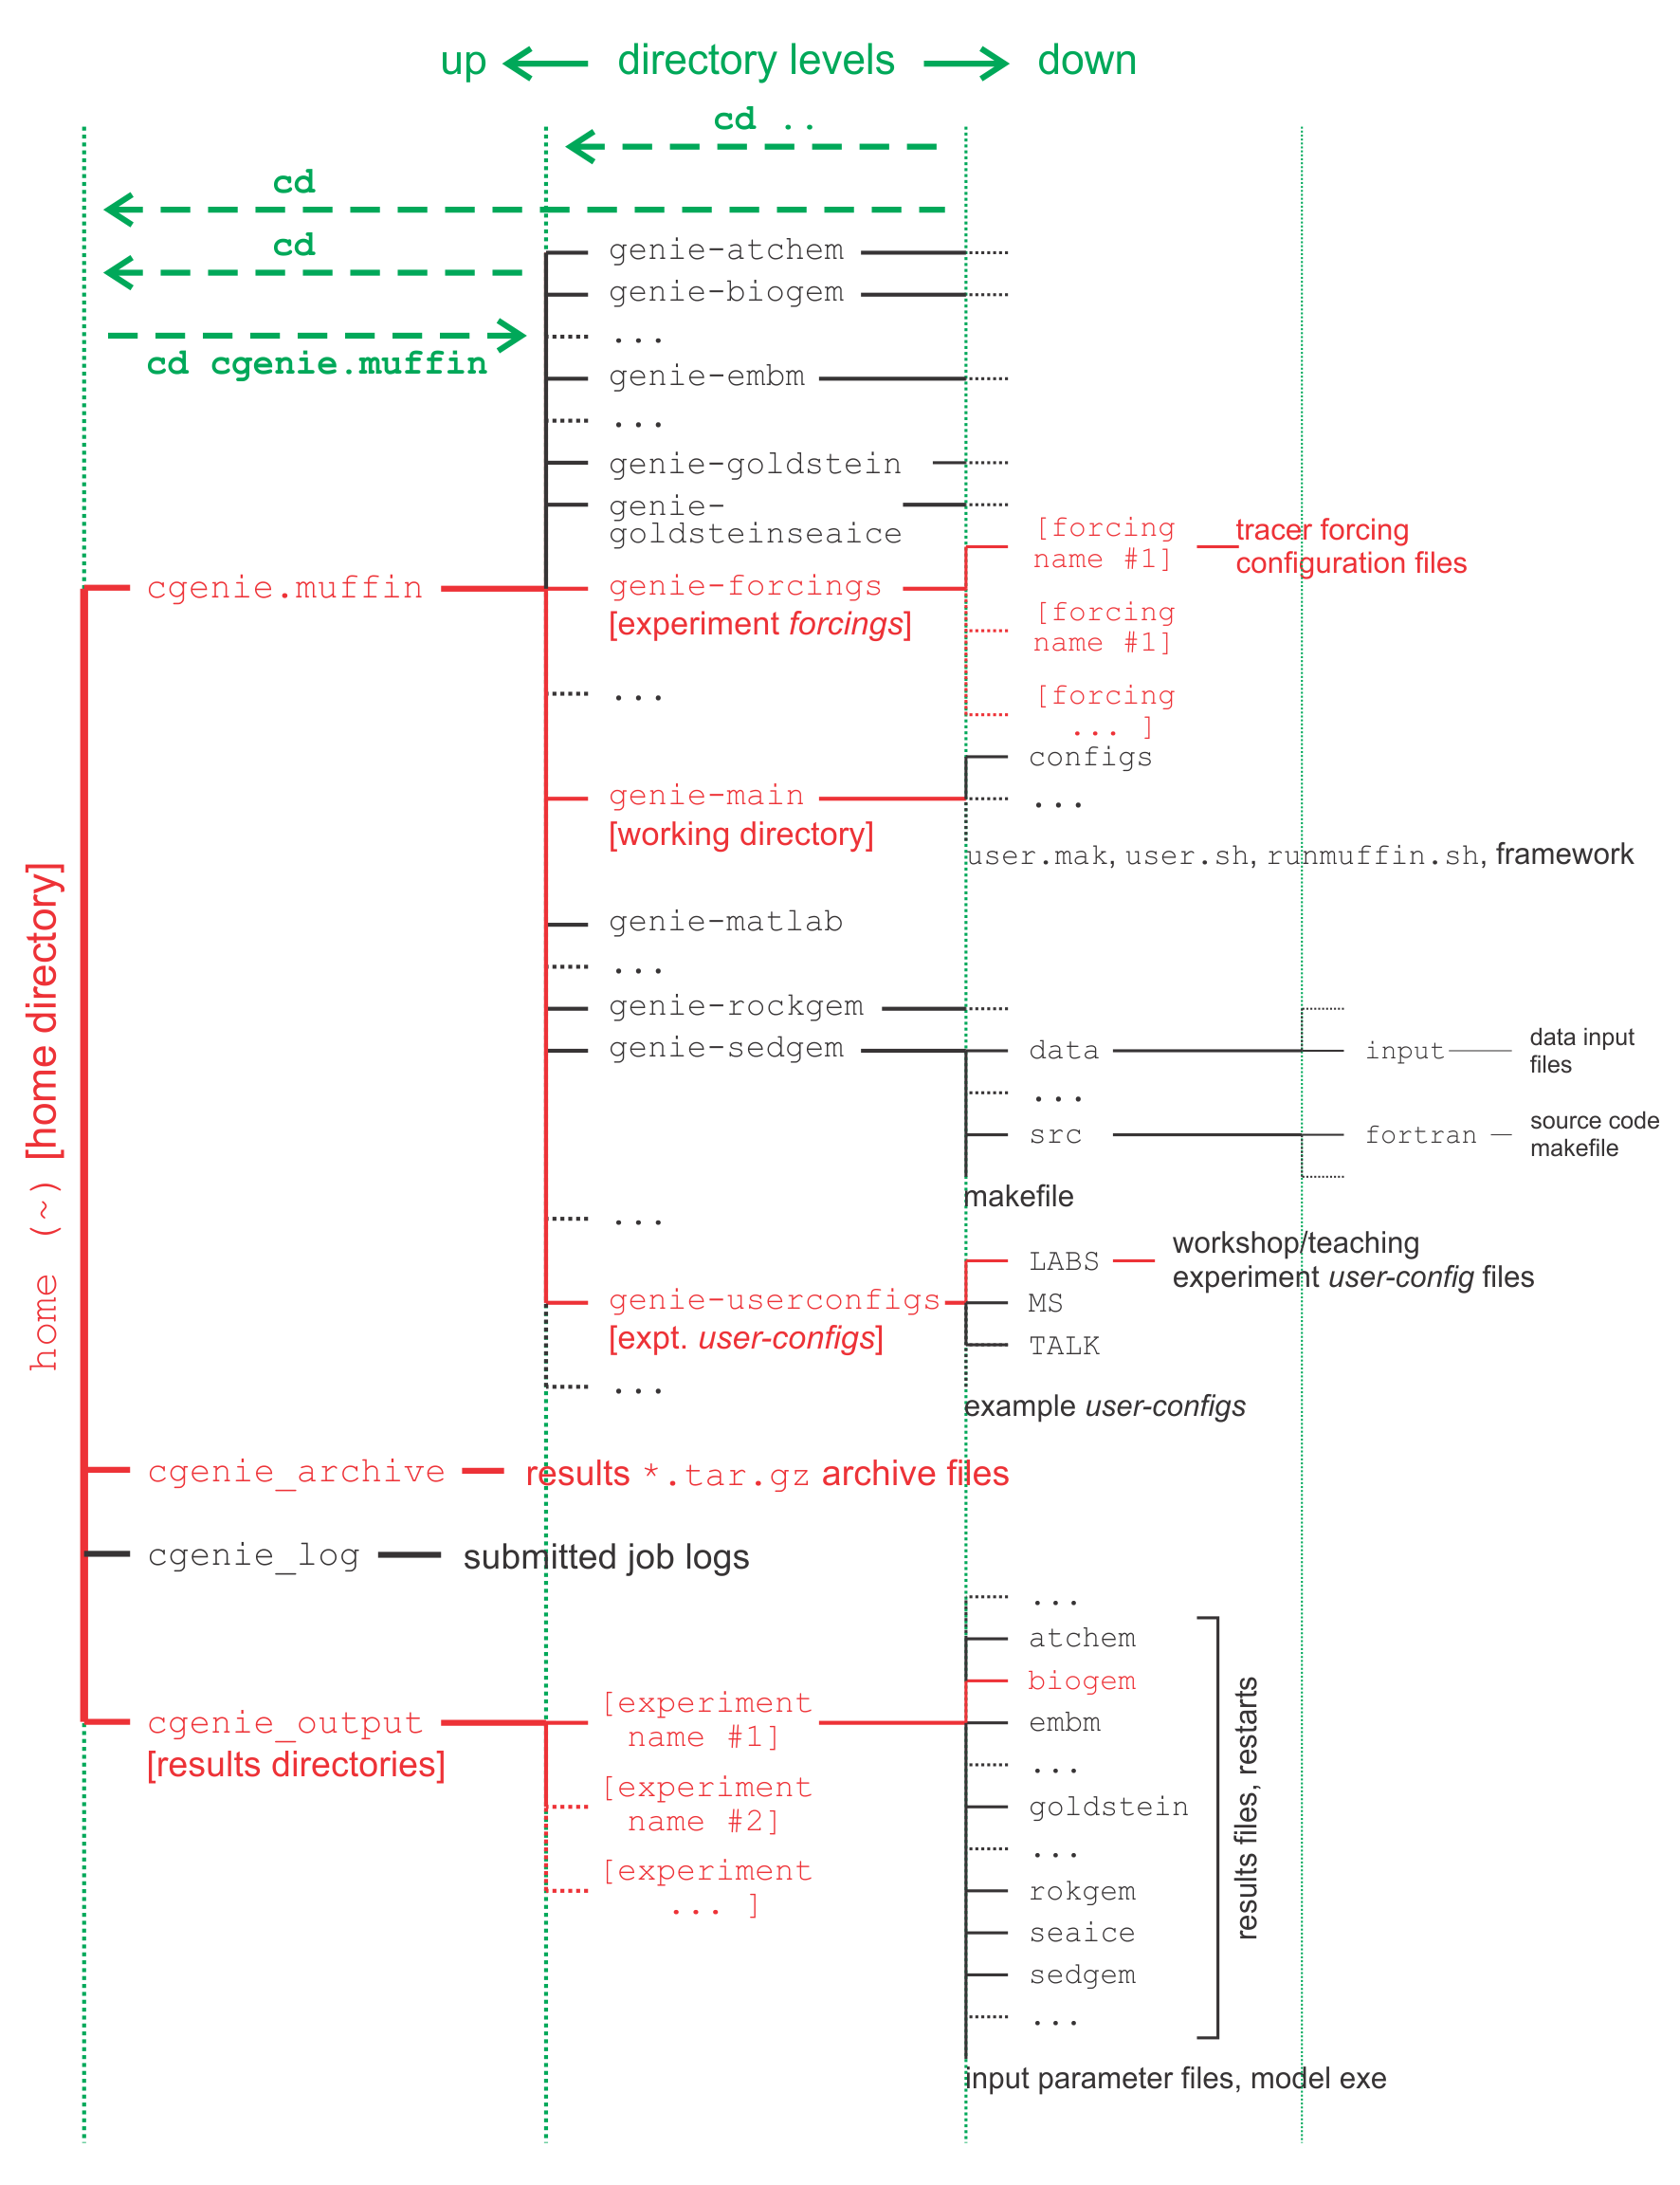
\includegraphics[width=\linewidth]{directories.png}
\caption{Directory structure of the \textbf{muffin} model. Highlighted in \textcolor{red}{red} are directories and sub-directories that you will need to access at some point. Vertical \textcolor[rgb]{0,0.501961,0}{green} lines designate directory levels, with example commands shown for moving between them.}
\label{fig:directories}
\end{figure}

%------------------------------------------------

\newpage

%------------------------------------------------

\section{Running the model}

The overall sequence of configuring and running \textbf{muffin}, is shown in Figure \ref{fig:chx-jobcreation}.

At the command-line (\texttt{\$}) in the genie-main directory (not your home directory), you will be entering in a command (\texttt{./runmuffin.sh}) together with a list of parameters that will be passed to the model, and as if by magic the model will run (or sometimes not). The form of the command you are going to be issuing is:

\vspace{-1mm}
\begin{verbatim}
$ ./runmuffin.sh #1 #2 #3 #4 (#5)
\end{verbatim}
\vspace{-1mm}

\noindent(\uline{don't type it yet}!)

\vspace{1mm}
The form of the command requires that you must list at least 4 parameters after \texttt{./runmuffin.sh}, separated by S P A C E S and on a single continuous line (even if it ‘wraps’ around across 2 lines of the screen).
These parameters are:

\vspace{2mm}
\begin{enumerate}[noitemsep]
\setlength{\itemindent}{.2in}
\item[\textbf{\#1}] ... is the name of the required base (or ‘basic’) configuration (‘\textit{base-config}’) of the model.
\item[\textbf{\#2}] ... is the name of the subdirectory (if any) containing the user configuration (‘\textit{user-config}’) file (i.e., the file containing the specification of a particular experiment). 
\item[\textbf{\#3}] ... is the name of the experiment itself. There must exist a file in the directory specified by parameter \#2 (\texttt{LABS}) with exactly the same name as you enter here for parameter \#3 (i.e. parameter \#3 points to a file in the directory given by parameter \#2).
\item[\textbf{\#4}] ... is the run length of the experiment in years – this must be entered as an integer.
\end{enumerate}

There is also one optional (5th) parameter (described later).

\vspace{1mm}
\noindent\rule{4cm}{0.1mm}
\vspace{2mm}

\noindent As an example of running the \textbf{muffin} Earth system model:

\vspace{2mm}
\begin{enumerate}[noitemsep]
\setlength{\itemindent}{.2in}
\item[\textbf{\#1}]: The base config is: \texttt{cgenie.eb\_go\_gs\_ac\_bg.worbe2.BASE}
\item[\textbf{\#2}]: The user config directory is: LABS
\item[\textbf{\#3}]: The user config file (the experiment name) is: \texttt{LAB\_0.EXAMPLE}.
\item[\textbf{\#4}]: Run the experiment for ten years: 10
\item[\textbf{\#5}]: (There is no restart file, and so no 5th parameter needs to be passed …)
\end{enumerate}

The full command for your first example experiment, which you are going to issue from the \texttt{\~}\texttt{/cgenie.muffin/genie-main} directory, then looks like:

\vspace{-1mm}
\begin{verbatim}
$ ./runmuffin.sh cgenie.eb_go_gs_ac_bg.worbe2.BASE LABS LAB_0.EXAMPLE 10
\end{verbatim}
\vspace{-1mm}

\noindent(\uline{you can try it now}!)

\vspace{2mm}
REMEMBER: This must be entered on a single CONTINUOUS LINE. The (single) S P A C E S are vital. Take care not to confuse an el (‘\texttt{l}’) with a one (‘\texttt{1}’) when typing this in ... (it is a ‘one’ here).

\vspace{1mm}
\noindent\rule{4cm}{0.1mm}
\vspace{2mm}

\noindent What should happen is: First, you will end up twiddling your thumbs a while, as all the components of \textbf{muffin} are compiled from the raw source code (\textbf{FORTRAN}). When it has finished doing this, the model will initialize and carry out some brief self-checking. Only then will it start actually ‘running’ and doing something, starting with a header describing the columns of numbers that follow:

\newpage

\begin{itemize}
\item[] \texttt{model year}  -- ... guess!
\item[] \texttt{ice(\%)} -- global sea-ice fraction (\%)
\item[] \texttt{<SST>} -- global sea surface temperature ('SST') $^{\circ}$C
\item[] \texttt{<SSS>} -- global sea surface salinity ‘SSS’ (\%\textit{o})
\end{itemize}

The choice of what information to display on screen as the model is running is rather arbitrary, but the chosen metrics do tend to summarize some of the main properties of the climate system and carbon cycle – for my own personal convenience rather than reflecting any fundamental scientific truth ... you may also see columns of information for: 

\begin{itemize}
\item[] p\(CO_{2}\)(uatm) -– mean atmospheric CO\(_{2}\) concentration (in units of \(\mu\)atm)
\item[] \(\delta^{13}CO_{2}\)  – mean \(\delta^{13}C\) value of atmospheric CO\(_{2}\) (\%\textit{o}) (NOTE: only if \(^{13}C\) tracer is selected)
\item[] \texttt{<DIC>} -- global mean ocean dissolved inorganic carbon (DIC) concentration (\(\mu\)mol kg-1)
\item[] \texttt{<ALK>}   – global mean ocean alkalinity (ALK) concentration (\(\mu\)eq kg-1) and in experiments with a modern continental configuration, also:
\item \texttt{AMO(Sv)} -- Atlantic meridional overturning circulation (Sv)
\end{itemize}

This information is reported at the same intervals as time-series data (see later and/or refer to the User Manual) is saved and is indicated by: 

\vspace{-2mm}
\begin{verbatim}
>>> SAVING BIOGEM TIME-SERIES AVERAGE CENTERED @ year :
\end{verbatim}
\vspace{-2mm}

Interleaved between these lines are lines reporting the saving of time-slice data (the 2- and 3-D model states – more of which later as well as in the User Manual). These appear as:

\vspace{-2mm}
\begin{verbatim}
>>> SAVING BIOGEM TIME-SLICE AVERAGE CENTERED @ year:
\end{verbatim}
\vspace{-2mm}

You can stop the model at any point (all data up to that time will have been saved) by hitting: \textsf{<Ctrl-C>} (\textsf{CONTROL} key + ‘\textsf{C}’ key).

Just from examining the screen output: how close to steady state does the system appear to have come after just 10 years? i.e., do SST and/or sea-ice extents appear to be converging towards stable (constant) values? This will be an important question to think about later on: ‘has the model reached steady-state (and does it matter)?’

In this example, the output should look something like the following:

\newpage

\footnotesize
\begin{verbatim}

 *******************************************************
 *** Initialisation complete: simulation starting ...
 *******************************************************
    
      model year  * pCO2(uatm)   d13CO2  *  AMO(Sv)  ice(%)   <SST>   <SSS>  *  <DIC>(uM)  <ALK>(uM)
  
 $N$        0.00       278.000   -6.500       0.000   0.000  -0.000  34.900      2244.000   2363.000
 >>> SAVING BIOGEM TIME-SLICE AVERAGE CENTERED @ year  :        0.500
 >>> SAVING BIOGEM TIME-SERIES AVERAGE CENTERED @ year :        0.500
 $N$        1.00       279.960   -6.598      13.613   0.744   2.509  34.901      2241.498   2363.111
 >>> SAVING BIOGEM TIME-SLICE AVERAGE CENTERED @ year  :        1.500
 >>> SAVING BIOGEM TIME-SERIES AVERAGE CENTERED @ year :        1.500
 $N$        2.00       279.525   -6.580      12.828   3.499   4.471  34.901      2240.173   2363.135
 >>> SAVING BIOGEM TIME-SERIES AVERAGE CENTERED @ year :        2.500
 $N$        3.00       279.258   -6.568      11.695   5.028   5.996  34.901      2239.169   2363.161
 >>> SAVING BIOGEM TIME-SERIES AVERAGE CENTERED @ year :        3.500
 $N$        4.00       279.044   -6.558      10.444   5.929   7.209  34.901      2238.354   2363.191
 >>> SAVING BIOGEM TIME-SLICE AVERAGE CENTERED @ year  :        4.500
 >>> SAVING BIOGEM TIME-SERIES AVERAGE CENTERED @ year :        4.500
 $N$        5.00       278.899   -6.551       9.380   6.191   8.156  34.902      2237.664   2363.220
 >>> SAVING BIOGEM TIME-SERIES AVERAGE CENTERED @ year :        5.500
 $N$        6.00       278.777   -6.545       8.500   6.623   8.975  34.902      2237.069   2363.246
 >>> SAVING BIOGEM TIME-SERIES AVERAGE CENTERED @ year :        6.500
 $N$        7.00       278.680   -6.541       7.922   6.629   9.637  34.903      2236.548   2363.267
 >>> SAVING BIOGEM TIME-SERIES AVERAGE CENTERED @ year :        7.500
 $N$        8.00       278.601   -6.537       7.917   6.738  10.225  34.903      2236.087   2363.285
 >>> SAVING BIOGEM TIME-SERIES AVERAGE CENTERED @ year :        8.500
 $N$        9.00       278.528   -6.534       7.952   6.740  10.732  34.904      2235.682   2363.301
 >>> SAVING BIOGEM TIME-SLICE AVERAGE CENTERED @ year  :        9.500
 >>> SAVING BIOGEM TIME-SERIES AVERAGE CENTERED @ year :        9.500
 $N$       10.00       278.466   -6.531       8.025   6.694  11.176  34.904      2235.325   2363.314

 *******************************************************
  *** Simulation complete: shutdown starting ...
 *******************************************************

\end{verbatim}
\normalsize

\begin{figure}
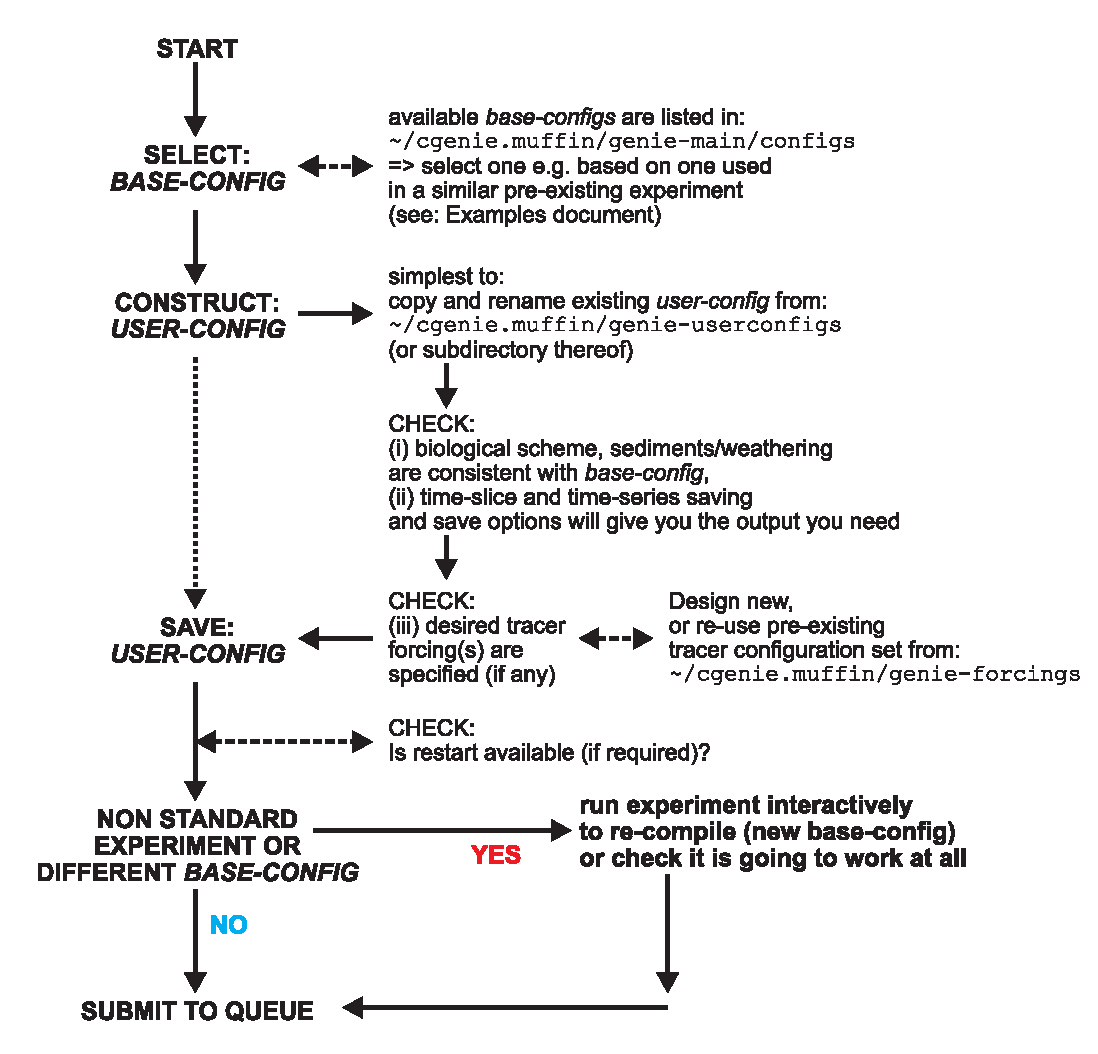
\includegraphics[width=0.9\textwidth]{chx-jobcreation.eps}\centering
\vspace{-0mm}
\caption{Schematic of the sequence-of-events in configuring and running an experiment.}
\label{fig:chx-jobcreation}
\end{figure}

%------------------------------------------------

\newpage

%------------------------------------------------

\section{Model output}

The first thing to note about output (i.e., saved results files) from \textbf{muffin} is that every science module saves its own results in its own sub-directory (and sometimes in very different and difficult-to-fathom ways …) – see Figure 1.1. All the sub-directories of results, plus copies of input parameters and the model executable, are gathered together in a directory that is assigned the same name as the experiment (== \textit{user-config} file name). The experiment results directories all live in:
\begin{verbatim}
~/cgenie_output
\end{verbatim}
and will be assigned a directory name something like:
\begin{verbatim}
LAB_0.EXAMPLE
\end{verbatim}
(this being the results directory name for an experiment called \texttt{LAB\_0.EXAMPLE}). Within this directory are each module’s results sub-directories.
We will primarily consider only results saved by the ocean biogeochemical module \textbf{‘BIOGEM’} (subdirectory: \small\texttt{biogem}\normalsize). The results files in this example will thus be found in:
\begin{verbatim}
~/cgenie_output/LAB_0.EXAMPLE/biogem
\end{verbatim}
\textbf{BIOGEM} has a flexible and powerful facility of saving results by means of spatially explicit ‘time-slices’, and as a semi-continuous ‘time-series’ of a single global (or otherwise representative mean) variable. In contrast, the atmospheric chemistry module '\textbf{ATCHEM}' does not save its own results (\textbf{BIOGEM} can save information about atmospheric composition and air-sea gas exchange) while the marine sediment module \textbf{SEDGEM} does save its own results, but only at the very end of a model experiment (\textbf{BIOGEM} can also save the spatial distribution of sediment composition as time-slices as well as mean composition as a time-series). Furthermore, to attain a common format for both ocean physical properties and biogeochemistry, \textbf{BIOGEM} can save a range of ocean results in addition to temperature and salinity, such as: velocities, sea-ice extent, mixed layer depth, convective frequency, etc.

%------------------------------------------------

\subsection{Time-slice output}

One of the most informative data sets that can be saved is that of the spatial distribution of properties (such as tracers or physical ocean attributes). However, saving full spatial distributions (e.g., a 36\(\times\)36\(\times\)8 array) for any or all of the tracers each and every time-step is clearly not practical; not only in terms of data storage but also because of the detrimental effect that repeated file access has on model run-time.
Instead, \textbf{BIOGEM} will save the full spatial distribution of tracer properties only at one or more predefined time points (in units of years). These are termed \textit{time-slices}. At the specified time points, a set of spatially-explicit data fields are saved for all the key tracer, flux, and physical characteristics of the system. However, rather than taking an instantaneous snapshot, the time-slice is constructed as an average over a specified integration interval (the default is set to 1.0 years, i.e. an annual average). \textbf{BIOGEM}  assumes that the specified time point represents the mid-point of the (annual) average with the results that output years end up being reported as e.g.,
\begin{verbatim}
0.5
1.5
2.5 
4.5
…
\end{verbatim}
(the mid-points of averages made over the intervals: 0-1, 1-2, 2-3, 4-5 years, etc.).

%------------------------------------------------

\subsection{Time-series output}

The second data format for model output is much more closely spaced in time. Model characteristics must then be reducible to a single meaningful variable for this to be practical (i.e., saving the time-varying nature of 3-D ocean tracer distributions is not). Suitable reduced indicators would be the total inventories in the ocean and/or atmosphere of various tracers (or equivalently, the mean global concentrations / partial pressures, respectively). Like the time-slices, the data values saved in the time-series files represent averages over a specified integration interval (the default is set to 1.0 years (annual average) but the results are reported with respect to the mid-point of the average which is where the ‘.5’ bits come in again).

%------------------------------------------------

\subsection{File naming convention}

The \texttt{biogem} results directory will contain files with names of the form:

\begin{itemize}[noitemsep]
\setlength{\itemindent}{.2in}
\item  \texttt{\_restart.nc} (is the re-start file created form the run you have just complete, and can be ignored).
\item \texttt{biogem\_series\_*.res} – these are the time-series files (in ASCII / plain text format).
\item \texttt{biogem\_year\_*\_diag\_GLOBAL.res} – these contain (global diagnostics) summary information and are saved at the same frequency as the time-slices (also as ASCII / plain text).
\item \texttt{fields\_biogem\_2d.nc} – 2-D fields of ocean and atmosphere properties, as NetCDF.
\item \texttt{fields\_biogem\_3d.nc} – 3-D fields of ocean properties, as NetCDF.
\end{itemize}

%------------------------------------------------

\newpage

%------------------------------------------------

\section{Viewing model output}

%------------------------------------------------

\subsection{Time-series output}

A descriptive summary of all the time-series (\texttt{biogem\_series\_*.res}) data files is given in the \textbf{muffin} User Manual if you are really that bored. The files of most immediate use/relevance are:

\begin{itemize}[noitemsep]
\setlength{\itemindent}{.2in}
\item \texttt{biogem\_series\_atm\_humidity.res}  - mean atmospheric (surface) humidity
\item \texttt{biogem\_series\_atm\_temp.res}      - mean atmospheric (surface) air temperature
\item \texttt{biogem\_series\_misc\_opsi.res}     - min/max overturning stream-function values (e.g. AMOC)
\item \texttt{biogem\_series\_misc\_seaice.res}   - mean ocean sea-ice cover and thickness
\item \texttt{biogem\_series\_ocn\_sal.res}       - mean ocean surface and whole ocean salinity
\item \texttt{biogem\_series\_ocn\_temp.res}      - mean ocean surface and whole ocean temperature
\end{itemize}

\vspace{1mm}
\noindent\rule{4cm}{0.1mm}
\vspace{2mm}

\noindent One way of viewing the contents of files is to change directory to the experiment results directory and opening the file in the file editor. But that is not so much fun.

Instead – change to the experiment results directory and then to the \texttt{biogem} sub-directory in the Secure File Transfer Client, and try double-clicking (if you have set up the \textbf{WinSCP} preferences correctly) or right-mouse-button-clicking (the then Edit with) on one of the .res files (listed above). For \texttt{biogem\_series\_ocn\_temp.res}, you should see 2 columns – time and mean (whole) ocean temperature ($^{\circ}$C). (However, in subsequent exercises a fuller output will be created with additional columns, with one for mean surface ocean temperature ‘SST’ ($^{\circ}$C) as well as mean benthic (bottom water) temperature ($^{\circ}$C)). Other results files may differ in the numbers of columns but all should be identifiable from the header information.

Note: \textbf{WinSCP} does not automatically refresh the directory listing. If you cannot see the results sub-directory with the experiment name you have just run, 99 times out of 100, it is because the display of the \textbf{WinSCP} needs to be refreshed -- there is an icon at the top of the program window or hit the ‘\textsf{F5}’ key.

\vspace{1mm}
\noindent\rule{4cm}{0.1mm}
\vspace{2mm}

\noindent For your information and edification (only): \textbf{Excel}, or \textbf{MUTLAB} if you prefer, can be used to graph the time-series results. Either way you will have to deal with the header line(s) that are present at the top of the file (and preceding the rows of data).

In \textbf{Excel}: Choose \textsf{File} then \textsf{Open}.  You will want to select \textsf{Files of Type} ‘\textsf{All Files (*.*)}’. In the \textsf{Text Import Wizard} window you can request that \textbf{Excel} skips the first few lines to start the import on the 2nd or 3rd line of the text file. Alternatively: set an appropriate column width manually in \textbf{Excel} to ensure that the columns of data are correctly imported.

\textbf{MUTLAB} will ignore lines starting with a \textsf{\%}, which the time-series starts with. However, it may be that the header line wraps-around and there is in effect a 2nd header line but without a \textsf{\%}. In this case, extra care (or a quick edit of the header in the ASCII file) will be required to load the data into \textbf{MUTLAB}.

%------------------------------------------------

\subsection{2- and 3-D time-slice output}

For the time-slice NetCDF (*.nc) files you will be using a program called \textbf{Panoply}. If you want your own (FREE!) copy of this utility, you can get it here (and is available for: \textbf{Windoz}, \textbf{Mac}, and linux operating systems): http://www.giss.nasa.gov/tools/panoply/.

\noindent When you open the NetCDF file, you will be presented with a ‘\textsf{Datasets and Variables}’ window (on the left hand side of the application window). This contains a list of all the parameters available that you can display. You will find that the ‘\textsf{Long Name}’ description of the variable will be the most helpful to identify the one you want. Simply double-click on a variable to display. For the 3-D fields you will be asked first whether you want a ‘\textsf{Longitude-Latitude}’ or ‘\textsf{Latitude-Vertical}’ plot (for the 2-D fields, the plot display will immediately open).
For the ‘\textsf{Longitude-Latitude}’ plots – there are multiple levels (depth layers) in the ocean - these data that can be plotted from the surface to the abyssal ocean.
For the ‘\textsf{Latitude-Vertical}' plots – there are multiple possible longitudes at which to plot slices. The default is the global mean meridional distribution. 
There is also an option for ‘\textsf{Longitude-Vertical}' plots (which we will not use).
For all three: there may be multiple time-slices (i.e., you can plot data saved from different years).
You can interpolate the data or not (often you may find that it is clearer not to interpolate the data but to leave it as ‘blocky’ colors corresponding to the resolution of the model), change the scale and colors, overlay continental outline, change the projection, etc etc. Grey cells represent ‘dry’ grid points, i.e., continental or oceanic crust.

NOTE: The default settings in \textbf{Panoply} can mislead:
\begin{enumerate}
\item By displaying the very 1st time-slice (often year mid-point 0.5) time-slice rather than the experiment end. (This can confuse as it can look like an experiment has not done anything!)
\item By interpolating the data (not always misleading). To remove interpolation, un-tick:
\\‘\textsf{Interpolate}’ in the ‘\textsf{Arrays}’ tab.
\item By displaying a global zonal mean by default when selecting \textsf{Latitude-Vertical} plots. Then, to further confuse you, by plotting the output up-side-down (to invert: in the ‘\textsf{Grid}’ tab, hit ‘\textsf{Swap B/T}’ (for swap bottom/top). 
\item By listing all ‘\textsf{Plottable variables}’ (option at the bottom of the window), when what you \textit{ideally} want are  the shorter and less confusing list of ‘\textsf{Georeferenced variables}’. 
\item In \textsf{Longitude-Latitude} plots, by overlaying the modern continental output. (\textbf{muffin} land is marked in grey.)
\item By fitting a scale to the plot when the display window is opened, but not changing the scale when e.g., time or depth is changed. (The point of confusion is that you can quickly move outside the scale and end up with all model points dark blue or red.) Re-fit the scale, or manually set limited, in the ‘\textsf{Scale}’ tab. 
So be careful when opening a new plot that you are looking at what you *think* you are looking at …
All the defaults can be changed via the ‘\textsf{Edit}’ drop-down menu and ‘\textsf{Preferences}’.
\end{enumerate}

\vspace{1mm}
\noindent\rule{4cm}{0.1mm}
\vspace{2mm}

\noindent Explore different data fields and play with different ways of displaying them. Aim for a set of display properties that show the information you are interested in / want to present in the clearest possible manner. Try different years (time-slice number), depth level (for a Latitude-Longitude plot), or longitude (for a vertical section).

\vspace{1mm}
\noindent\rule{4cm}{0.1mm}
\vspace{2mm}

\noindent To save plots in \textbf{Panoply}:
\small
\\\textsf{File}
\\\textsf{Save Image As …}
\normalsize
\\Then select the location, filename, and graphics format.

%------------------------------------------------

\newpage

%------------------------------------------------

\section{Submitting experiment ‘jobs’}

This bit is no particular fun at all, but it is a very handy ‘trick’ for running the model in the background, and maximizes drinking time in the bar vs. sat bored watching a computer screen :)

\vspace{1mm}
\noindent\rule{4cm}{0.1mm}
\vspace{2mm}

\noindent Running jobs interactively is all very well, but there are three important limitations:
(1) The connection between your terminal and the server computer running the model must remain unbroken. Anything more than a fleeting loss of internet connectively may result in the experiment terminating.
(2) You can only run one experiment at a time … unless you want to have thousands of separate terminal open …? I thought not …
(3) Any cluster or computer you are likely to be accessing using a shell will not have many computing cores itself, either because it is a single machine with only one or two processors, or if a cluster, by using a terminal you are running on the ‘head node’, which will have similar computing core limitations to running on a single machine. The more experiments you run simultaneously, the slower they will all run …

\vspace{1mm}
\noindent\rule{4cm}{0.1mm}
\vspace{2mm}

\noindent The alternative is to submit your experiment as a ‘job’ to a queuing system which then manages what compute resources are used to run the model. Once you have submitted the experiment, that is it – you can go straight to the pub :)

For example -- to run the same experiment as before (\texttt{LAB\_0.EXAMPLE}) for maybe 100 years (or even longer if you wish – I am just pulling factors of 10 out of thin air here) but now submit the experiment as a job to the cluster queue, type:
\vspace{-1mm}
\small\begin{verbatim}
$ qsub -q dog.q -j y -o cgenie_log -V -S /bin/bash runmuffin.sh
  cgenie.eb_go_gs_ac_bg.worbe2.BASE LABS LAB_0.EXAMPLE 100
\end{verbatim}\normalsize
\vspace{-1mm}

\noindent(Again: SINGLE, CONTINUOUS LINE.) Here, the particular queue name is \textsf{dog}.

Note that now you should omit the ‘\texttt{./}’ bit before \texttt{runmuffin.sh}.
(If you are interested (I know that you are not): the options following \texttt{qsub} and before \texttt{runmuffin.sh} do things like re-directing screen output and error messaging to a file and specify which linux ‘shell’ to assume. It is even possible to receive an email when the job is done :) )
The status of the cluster queue and how you experiment job is getting on (e.g., “Is it finished yet?”) can be checked by typing: 
\vspace{-1mm}
\small\begin{verbatim}
$ qstat -f
\end{verbatim}\normalsize
\vspace{-1mm}
(\texttt{qstat -f -u "*"} will show all jobs on the cluster.)

After submitting an experiment, you receive a job number. This number appears in the first column in the queue status information when you issue a qstat –f command. You should see your job appear on one of 6 compute nodes, numbered 0-0 to 0-5), although it might briefly reside as a ‘PENDING JOB’. For each node, there are multiple processing cores (depending on the specific cluster and queue), meaning that multiple instances of \textbf{muffin} can run simultaneously on each node. For an 8-level ocean based configuration of \textbf{muffin}, being run for 100 years, the job should remain there in the queue for a few minutes before ‘disappearing’ (your clue that it has finished, or died\footnote{If your experiment appears on the queue but vanishes after a few seconds, it has most likely died :(} …). If you periodically re-issue a \texttt{qstat –f} command you can follow your job’s progress.

A rough rule of thumb is that 8-level ocean \textbf{muffin} @ a horizontal grid resolution of 36x36 will simulate about 1000 years per CPU hour. The 16-level version (which you will use later), runs at about 300-400 years per CPU hour.

\noindent \textbf{NOTE}: It may be that the \textbf{FORTRAN} compiler is not accessible by the computer nodes. The implication of this is that \textit{the \textbf{muffin} executable must be already compiled BEFORE a job is submitted to the queue}.

\noindent In other words; if you have just changed the model resolution or continental configuration, or number of tracers (i.e. changed the \textit{base-config}) or issued a \texttt{make cleanall} command you MUST briefly run your desired experiment (or equivalent) interactively (i.e., in the shell window) to ensure that everything is correctly compiled. For instance, either run the experiment for a couple of years or start the experiment for the desired full duration, but 'kill it' (Ctrl-C) once the experiment is running successfully.

%------------------------------------------------

\newpage

%------------------------------------------------

\section{‘Restarts’}

Not much fun here either … but again – an important and time-saving (== increased drinking time!) modelling technique to learn to use.

By default, model experiments start from ‘cold’, i.e., the ocean is at rest and uniform in temperature and salinity while the atmosphere is uniform in temperature and humidity. All biogeochemical tracers in the ocean have uniform concentrations and/or are zero and there are no biogenic materials in deep-sea sediments. From this state it will take several thousand years (kyr) for the climate system to reach steady-state, and closer to 5 kyr (or more) for ocean biogeochemical cycles and atmosphere \(CO_{2}\) to reach steady-state, and exceeding 100 kyr for sediment composition to re-balance weathering ... Reaching this the equilibrium state is called the ‘\textit{spin-up}’ phase of the model.
There is evidently little point in repeating the \textit{spin-up} for each and every model experiment that are similar except in a single detail (e.g., testing a variety of different \(CO_{2}\) emissions scenarios all starting from current year 2012 conditions). A facility is thus provided for requesting that a ‘\textit{re-start}’ is used – starting a new experiment from the end of a previous one, usually a \textit{spin-up} that has been run explicitly for the purpose of generating a starting point (\textit{re-start}) of the system at steady-state (equilibrium) for subsequent experiments to continue on from.
It is important to note that there is nothing special about a \textit{re-start} – it is simply an experiment that you have already run. Equally, there is nothing special about the \textit{re-start}s you will download next – these you could have generated yourself – it simply saves time to have them provided.

\vspace{1mm}
\noindent\rule{4cm}{0.1mm}
\vspace{2mm}

\noindent To experiment with using a \textit{re-start}, you will first need to download a file that has been created (a pre-run 10,000 year spin-up). To fetch this: Change to the \texttt{cgenie\_output} directory (perhaps by going ‘home’ first (\texttt{cd} \textsf{<Enter>}), and then changing to \texttt{cgenie\_output} – refer to linux commands HOW-TO and Figure 1.1), and type:

\vspace{-2mm}
\begin{verbatim}
$ wget http://www.seao2.info/cgenie_output/LAB_0.SPIN.tar.gz
\end{verbatim}
\vspace{-2mm}

This downloads an archived/compressed copy of the restart from a location on the interweb. Extract the contents of this archive by typing:

\vspace{-2mm}
\begin{verbatim}
$ tar xfzv LAB_0.SPIN.tar.gz
\end{verbatim}
\vspace{-2mm}

Finally, change directory back to \texttt{cgenie.muffin} and then \texttt{genie-main} so that you are ready to run the model (the model is *always* run from \texttt{cgenie.muffin/genie-main}).

\vspace{1mm}
\noindent\rule{4cm}{0.1mm}
\vspace{2mm}

\noindent A \textit{re-start} can be requested in running an experiment by setting the 5th and last (optional) parameter when entering in the \texttt{runmuffin.sh} command. A spin-up of the climate state is provided: \texttt{LAB\_0.SPIN} which you have just unpacked to the \texttt{cgenie\_output} results output directory.
Create a new (\textit{user-config}) experiment configuration file in the: \linebreak \texttt{~/cgenie.muffin/genie-userconfigs/LABS} directory by using the given file \texttt{LAB\_0.EXAMPLE} as a template (no parameter changes need to be made yet). You can make copies (cp command) of the experiment configuration files (e.g., \texttt{LAB\_0.EXAMPLE}) and assign them different names, e.g., twilight, rarity, applejack …. (ideally, use a name that helps you remember what the experiment did). Or … if you and the linux command lines are simply not BFFs, you can drag the \textit{user-config} file (\textsf{\footnotesize LAB\_0.EXAMPLE}) you want to use as a template to your local PC (/Mac) directory in the file transfer window, rename it either in the file transfer program or e.g., via the Windoz file-manager (e.g., to \texttt{LAB\_0.NEW}), and drag it back to the cluster directory \footnote{\texttt{~/cgenie.muffin/genie-userconfigs/LABS}} again.
You specify the use of the restart state by adding the restart experiment name as the 5th parameter, e.g.:

\vspace{-2mm}
\small\begin{verbatim}
$ ./runmuffin.sh cgenie.eb_go_gs_ac_bg.worbe2.BASE LABS LAB_0.NEW 100 LAB_0.SPIN
\end{verbatim}\normalsize
\vspace{-2mm}

The run-time output should now look noticeably different. There should be no (or perhaps just very little) drift in any of the various variable values outputted to the screen – this is because you have (re-)started from the end of a run that had already ready an equilibrium, steady-state.

%----------------------------------------------------------------------------------------
%       CHAPTER 2
%----------------------------------------------------------------------------------------

\cleardoublepage

\chapterimage{Figure-1-The-image-of-an-ice-encased-Earth-a-Snowball-Earth-with-oases-of-open-water-on.png} % Chapter heading image

\chapter{Climate dynamics \& experimental design}

\hfill \break

\noindent Stuff to keep in mind:

\begin{itemize}
\item Models ARE NOT the ‘real World’ (it is going to be pretty obvious this is the case here).
\item Don’t believe what you read in Nature or Science.
\end{itemize}

%------------------------------------------------

\newpage

%------------------------------------------------

\section*{Readme}

You will need to download a new \textit{restart} file prior to embarking on the snowball Earth experiments.
To fetch this: change to the \texttt{cgenie\_output} directory, and type (or copy and paste carefully from this PDF ...):
\vspace{-2mm}
\begin{verbatim}
$ wget http://www.seao2.info/cgenie_output/LAB_1.SPIN.tar.gz
\end{verbatim}
\vspace{-2mm}

This downloads an archived/compressed copy of the experiment \texttt{LAB\_1.SPIN} – effectively, just an experiment (spin-up) that has been run for 5,000 years for you. Extract the contents of this archive by typing:
\vspace{-2mm}
\begin{verbatim}
$ tar xfzv LAB_1.SPIN.tar.gz 
\end{verbatim}
\vspace{-2mm}

A new experiment results directly will then appear as if you had just run the entire 5,000 year experiment yourself, and you could in fact have done so (remember to refresh the \textbf{WinSCP} directory view window if you are using this particular software, or it might appear that nothing has been extracted).

You’ll then need to change directory back to \texttt{genie-main} to run the model.

%------------------------------------------------

\newpage

%------------------------------------------------

\section{Brrrrrrrrrrrr – it’s chilly on ... snowball Earth!}

To illustrate how ‘easy’ it can be to configure an Earth system / climate model such as \textbf{muffin} and explore the behavior of the Earth system and its response to perturbation – you are going to induce an extreme cooling of the climate system and see what happens. Solar output was weaker during the late Neoproterozoic, a time when the Earth experienced a series (2 ish) of extreme glaciations. Thus, having a mild climate state to start with must have been dependent on sufficient \(CO_{2}\) and/or \(CH_{4}\) in the atmosphere and hence presumably highly elevated compared to the modern World ... sort of opposite to the problem we have today …

\vspace{1mm}
\noindent\rule{4cm}{0.5pt}
\vspace{2mm}

\noindent You are going to be running experiments in a similar manner to before, and using the \textit{re-start} experiment that you downloaded:
\vspace{-1mm}
\small\begin{verbatim}
$ ./runmuffin.sh cgenie.eb_go_gs_ac_bg.woreq1.NONE LABS LAB_1.EXAMPLE 100 LAB_1.SPIN 
\end{verbatim}\normalsize
  
\noindent But ... rather than use the provided experiment configuration file \texttt{LAB\_1.EXAMPLE} (which is provided for you), why not get into the habit of creating new and uniquely named \textit{user-config} files (no harder than copying it and renaming it!). If you keep using the same experiment name, the results will be over-written each time, while having  2 (or more) experiments running simultaneously with exactly the same name causes havoc as they try and over-write each others results files in a somewhat entertaining but ultimately useless way.

Overall: your task in this exercise will be to determine the radiative forcing (or p\(CO_{2}\) equivalent) threshold required to drive the climate system into a full ice-covered ocean (snowball Earth) state. (Read the \textit{Hyde et al.} [2000] paper.)

Useful 2-D (netCDF—Panoply) variables to view are surface air temperature and sea-ice extent (and/or thickness). Ocean surface temperature and salinity can be viewed in the 3-D NetCDF results file.

Time-series (ASCII .res files) are useful for providing simple mean indicators of global climate such as global ocean fractional sea-ice covered. 

Note that the model configuration of an idealized super-continent, positioned symmetrically about the Equator, is pretty unrealistic. But the further you go back in time, the more uncertain it becomes as to exactly where and in what orientation the continents were. Sometimes modelers have to resort to somewhat idealized experiments if the uncertainties are too great. In addition, one can conduct sensitivity experiments to test whether the continental configuration is important to the results. For instance, \textit{Hoffman and Schrag} [2002] discuss the potential importance of continental configuration, while the entire hypothesis of \textit{Donnadieu et al.} [2004] rests on specific details of the continental configuration being realistic.

For this configuration, the solar constant is set weaker than modern to reflect the fact that the Sun’s output has increased with time and during the Neoproterozoic the solar constant would have been ca. 5\% weaker. This is set by the model \textit{parameter}:

\vspace{-1mm}
\begin{verbatim}
ma_genie_solar_constant= 1285.92
\end{verbatim}
\vspace{-1mm}

\noindent which is set at the top of the provided \textit{user-config} file. (For reference, the modern value is \( 1368 Wm^{-2}\).)

\vspace{1mm}

Other questions to think about with regards to numerical modeling (and this experiment) are:

\begin{itemize}[noitemsep]
\setlength{\itemindent}{.2in}
\item  (Is the model configuration and experimental design ‘realistic’ ... ?)
\item  What is ‘missing’ in the model and what might the implications for your predictions and conclusions be? For example, there is no land-surface scheme (and hence no concept of ‘snow’) in this particular configuration.
\item Are the simulations being run for sufficiently long? Why not if not (i.e., justify your choices of parameter values and experimental assumptions)? How might the results and conclusions be biased (if at all)?
\item How would you test model predictions and your overall conclusions?
\item How could the experimental design be improved?
\end{itemize}

\vspace{1mm}
\noindent\rule{4cm}{0.5pt}
\vspace{2mm}

\noindent To search for the atmospheric \(CO_{2}\) concentration (or rather, radiative forcing equivalent) that would lead to a ‘snowball Earth’ state in the Neoproterozoic and answer the question:
‘How low does \(CO_{2}\) have to be to trigger a ‘snowball’?’
you are going to edit the file that controls the specific details of the experiment -- the \textit{user-config} file. From the \texttt{genie-userconfigs/LABS} directory, open one of the snowball experiments in your preferred  text editor. At the top of the file you should see something like:

\vspace{-2mm}
\small\begin{verbatim}
#
#
# --- CLIMATE ---------------------------------------------------------
#
…
# scaling for atmospheric CO2 radiative forcing, relative to 278 ppm
ea_radfor_scl_co2=20.0
\end{verbatim}\normalsize
\vspace{-2mm}

Each line that is not commented out (i.e., no \#) contains a \textit{parameter} name and assigned value pair, with the format:
\vspace{-2mm}
\begin{verbatim}
PARAMETER=VALUE
\end{verbatim}
\vspace{-2mm}
The value of each parameter can be edited to form a new experiment. (Additional parameter value specifications can also be added, or existing ones deleted.) In this example, the line: 
\vspace{-2mm}
\begin{verbatim}
ea_radfor_scl_co2=20.0
\end{verbatim}
\vspace{-2mm}
specifies a radiative forcing of climate by \(CO_{2}\) equivalent to x20 modern (20x278 = 2560 ppm). If you instead wrote: 
\vspace{-2mm}
\begin{verbatim}
ea_radfor_scl_co2=1.0
\end{verbatim}
\vspace{-2mm}
this would give you a modern (x1, or 1x278 = 278 ppm) radiative forcing. (Technically: the pre-industrial \(CO_{2}\) value rather than ‘modern’ \textit{per se.})
Note: \(CO_{2}\) is not being explicitly modeled in this experiment, but the long-wave radiative forcing associated with a specified concentration of \(CO_{2}\) (in ratio to modern) is being set instead.

Edit the value of \texttt{ea\_radfor\_scl\_co2} (lower or higher) and save the file. Re-run the experiment to see whether sea-ice extent is approaching a new steady state. You may want to try even longer simulations (than 100 years) if it becomes clear that the model is still far from steady-state. You can judge how close to equilibrium things have got by following (and/or plotting) the evolution of e.g., global surface air temperature or sea-ice extent (both time-series files).

HINT: Submitting the experiments to the cluster will allow you to run many many experiments (i.e. each with a different radiative forcing value) simultaneously.

\vspace{1mm}
\noindent\rule{4cm}{0.5pt}
\vspace{2mm}

\noindent For each experiment you want to be assessing how far towards the Equator the sea-ice limit encroaches through some of the \textit{time-series} and \textit{time-slice} files or even the on-screen summary lines (assuming running interactively rather than via a job submission to the cluster queue). Informative \textit{time-series} variables include (but not necessarily be limited to): atmospheric temperature and sea-ice cover. (Sea-ice thickness, on account of the simple physics in the model, low resolution and long time-step, can fluctuate a little in area and volume at times.)

For the \textit{time-slice} data: atmospheric and ocean surface temperature and sea-ice extent (2-D biogem \textbf{NetCDF} file) may be informative.

HINT: Be careful with the ‘\textsf{Fit to data}’ scaling feature in \textbf{Panoply} – at near complete sea-ice cover, you may find Panoply scaling min and max sea-ice between 99.1 and 99.9\% or something. Specific fixed scale limits (e.g. 0 and 100) can be set instead.

In answering the question (‘How low does \(CO_{2}\) have to be to trigger a ‘snowball’?’), think about what an appropriate degree of accuracy might be for your experiments. Just because computer models generally calculate to around 16 significant places of precision, does not mean you have 16 significant figures of realism. For instance – how many significant figures is the solar constant quoted to and what do you think is the uncertainty in this? Harder to judge is how the assumed (incorrect) continental configuration creates additional uncertainty, or the simple physics assumed in the ocean or sea-ice, or lack of snow on land … 

\vspace{1mm}
\noindent\rule{4cm}{0.5pt}
\vspace{2mm}

\noindent Once you are happy about the controls on the snowball threshold try and answer the supplementary question:

\vspace{2mm}
\noindent \textit{How high does the (\(CO_{2}\)) radiative forcing have to be in order to escape from a snowball?}
\vspace{2mm}

Having determined the appropriate radiative forcing value required to create a snowball state, you can use that experiment as a \textit{re-start}, and hence carry out a series of experiments with increasing radiative forcing, all starting from the same snowball climate state you have just created. Defining the radiative forcing / climate path going out of a snowball would complete the hysteresis loop of \textit{Hyde et al.} [2000]. Note that a good \textit{re-start} is one for which the experiment did not sit too long in the snowball state before finishing (the more sea-ice thickness you create in the first experiment, the more you are going to have to melt in the next …). To achieve this, you can fine-tune the number of years the experiment is run, i.e. having determined the appropriate radiative forcing value required to create a snowball state, find out when in the experiment the snowball state first occurred, and then run a new experiment that finishes only a decade or so after the snowball is initiated.\footnote{You cannot select when the \textit{re-start} is saved – it is always saved at the end of an experiment.}

HINT: If you are having trouble deciding whether or not the snowball is heading in the right direction (i.e. towards an exit!), e.g. because sea-ice is always reported at 100\% (or close to), you can keep track of whether there is net melting or net freezing by following mean sea-ice thickness (m) as reported in the \texttt{biogem\_series\_misc\_seaice.res} time-series output file. Your indication of a melting snowball state is a progressive decline in mean thickness (a proxy for global ice volume). \uline{Note that you can open and review the results of \textit{time-series} files at *any* time during the experiment as the lines are written while the data for each time point is generated.}

Overall: think critically about the model configuration, the experimental design, and the nature of the scientific question (based on your background reading of snowball Earth). Some of the exploration/testing suggestions (above) may not necessarily give substantially different results. Such a finding would be as valid and interesting as determining an important dependence of a certain assumption, and would for instance indicate that the associated paleo uncertainties are not critical to model assessment of the question.

Always be prepared to justify all your choices for experimental design and model settings, e.g., range of radiative forcing assessed, continental configuration(s), solar forcing, use of re-starts (if any), run duration, etc. etc. etc. etc.

%------------------------------------------------

\newpage

%------------------------------------------------

\section{Further ideas}

%------------------------------------------------

\subsection{Feedback loop analysis}

To quantify the snowball Earth hysteresis loop in \textbf{muffin} as per Figure 2 in \textit{Hyde et al.} [2000] you will need to extract from the model ‘meaningful’ measures of climate (e.g., global surface air temperature, fractional sea-ice coverage) as a function of \(CO_{2}\) multiples, \(CO_{2}\) concentration, or (better) radiative forcing. For the latter, in \textbf{muffin}, the radiative forcing for a doubling of \(CO_{2}\) is set at: \(5.77 Wm^{-2}\). See: \textit{Myhre et al.} [1998] (Geophys. Res. Lett. 25, 2715–2718) and/or \textit{IPCC} [2007] for more on what radiative forcing is and how it is related to a relative change in \(CO_{2}\) concentration. Also, for making a comparison with \textit{Hyde et al.} [2000] -- for going into the snowball, note that they plot the change in radiative with a ‘cooling’ as positive (a bit daft). Their baseline radiative forcing state (an anomaly of \(0 Wm^{-2}\)) you might assume is equivalent to 278 ppm and hence \(\backsim\)130 ppm is an approximately halving of \(CO_{2}\) and hence creates \(\backsim5 Wm^{-2}\) of cooling. (You might prefer to plot the radiative forcing change as warming being positive, which makes rather more sense ...)

For coming out of a snowball, because the \(CO_{2}\) and hence radiative forcing threshold is so high as compared to going in, you may want to be creative in the plotting (assuming attempting to combine both thresholds into a single plot) and, for instance, one might break the scale between the low radiative forcing interval spanning going in and the high one spanning coming out.

Another example is as per Figures 3 and 4 in \textit{Stone and Yao} [2004] (Clim. Dyn. 22, 815–822) (although here it is the solar constant rather than long-wave radiation forcing that is being varied). So in fact, you could try varying the solar constant as an alternative to radiative forcing and hence be able to come up with a plot directly comparable to \textit{Stone and Yao} [2004].

%------------------------------------------------

\subsection{Continental configuration (1)}

It was mentioned earlier that the position of the continents is an area of modelling uncertainty and might be important. You can test for this. Four alternative \textit{base-configs} are provided, each defining a different continental configuration:

\vspace{1mm}
\begin{enumerate}[noitemsep]
\setlength{\itemindent}{.2in}
\item 
\begin{verbatim}
cgenie.eb_go_gs_ac_bg.wopol1.NONE
\end{verbatim}
 – a single polar super-continent, with an ocean resolution of 36x36 with 8 vertical levels. (Note potential ‘l’ and 1’1 confusion in ‘wopol1’.)
\item
\begin{verbatim}
cgenie.eb_go_gs_ac_bg.wopol2.NONE
\end{verbatim}
  – one continent at each pole, with an ocean resolution of 36x36 with 8 vertical levels.
\item
\begin{verbatim}
cgenie.eb_go_gs_ac_bg.woreq1.NONE
\end{verbatim}
  – a single Equatorially-centred super-continent, with an ocean resolution of 36x36 with 8 vertical levels. [current configuration]
\item 
\begin{verbatim}
cgenie.eb_go_gs_ac_bg.woreq2.NONE
\end{verbatim}
 – two continents straddling the Equator, with an ocean resolution of 36x36 with 8 vertical levels.
\end{enumerate}
\vspace{1mm}
   
You can use the given \textit{user-config} file (\texttt{LAB\_1.EXAMPLE}) as an experiment template, and any of the alternative configurations can be run very similarly to as per before, i.e.:

\vspace{-2mm}
\begin{verbatim}
$ ./runmuffin.sh cgenie.eb_go_gs_ac_bg.xxxxx.NONE LABS LAB_1.EXAMPLE 100
\end{verbatim}
\vspace{-2mm}

Note that you are using a different \textit{base-config} file name: \small\texttt{cgenie.eb\_go\_gs\_ac\_bg.xxxxx.NONE}\normalsize \\where \texttt{xxxxx} is one of: \texttt{wopol1}, \texttt{wopol2}, \texttt{woreq1}, or \texttt{woreq2}. 

\uline{Also note} that \uline{no} \textit{re-starts} are provided for any of these configurations. You may (or may not) want to create some (you will need to judge for yourselves how long to run the restart experiments for to achieve as close to steady-state as you think is ‘sufficient’). Recall again, that \textit{re-starts} are just ‘normal’ experiments that have already been run.
Be careful that when changing from one \textit{base-config} to another, the model re-compiles. Simply running the new configuration briefly is sufficient to ensure this. Experiments can then be safely submitted to a cluster queue, i.e. do not try and submit an experiment using a different \textit{base-config} straight to the cluster queue without having run it (or a short version of the experiment you want) interactively first (to ensure the model is re-compiled). This is also good practice – checking that a new sort of experiment and/or model configuration works as you intend and without hiccups.

%------------------------------------------------

\subsection{Continental configuration (2)}

Although much useful can be learned from conceptual configurations and Worlds regarding climate dynamics, it is invariably aesthetically more 'pleasing' to also test ideas in a more paleogeographically realistic configuration. Provided is a set of \textit{base-config} and \textit{user-config} files (plus associated boundary conditions) for the position of the continents and climate 635 millions years ago (635 Ma). For this:

The \textit{base-config} is named: \texttt{muffin.C.fm0635cb.NONE}

The \textit{user-config} is: \texttt{muffin.C.fm0635cb.NONE.SPIN}

NOTE that the \textit{user-config} file is now found in the directory:

\vspace{-2mm}
\begin{verbatim}
~\cgenie.muffin\user-configs\PALEO
\end{verbatim}
\vspace{-2mm}

\noindent so that you either need to specify this different (\texttt{PALEO}) directory when running \textbf{muffin}, or copy the \textit{user-config} file into \texttt{LABS}.

A \textit{re-start }experiment is provided called \texttt{muffin.CB.fm0635cb.NONE.SPIN} and which can be downloaded as per before:

\vspace{-2mm}
\begin{verbatim}
$ wget http://www.seao2.info/cgenie_output/muffin.CB.fm0635cb.NONE.SPIN.tar.gz
\end{verbatim}
\vspace{-2mm}

\noindent and unpacked by:

\vspace{-2mm}
\begin{verbatim}
$ tar xfzv muffin.CB.fm0635cb.NONE.SPIN.tar.gz
\end{verbatim}
\vspace{-2mm}

\noindent (Remember: you should be in the \texttt{cgenie\_output} directory when you do this downloading and unpacking.)

To run (e.g. for 100 years), following on from its \textit{re-start} (and leaving the \textit{user-config} in its \texttt{PALEO} directory):

\vspace{-2mm}
\begin{verbatim}
$ ./runmuffin.sh muffin.C.fm0635cb.NONE PALEO muffin.C.fm0635cb.NONE.SPIN
    100 muffin.CB.fm0635cb.NONE.SPIN
\end{verbatim}
\vspace{-2mm}

\noindent (\uline{all on one line})

NOTE that the \textit{base-config} and \textit{user-config} filenames start \texttt{muffin.C.} whereas the\textit{ re-start} filename starts \texttt{muffin.CB.} ... just to try and trip you up ...

%------------------------------------------------

\subsection{Geothermal heat input}

Finally, \textbf{muffin} will fairly happily build up sea-ice, apparently without limit (with the remaining wet ocean becoming progressively colder and more saline). In the real world, one might expect some sort of limit to the maximum thickness achieved as the heat diffusion across a progressively greater thickness of sea-ice approaches the heat input at the bottom of the ocean from geothermal energy. Different modes of ocean circulation are also possible if one considers heating from the bottom as well as cooling (and brine rejection) from the top and which might affect the entry into or exit from a snowball state.

In the experimental setup you have been given, a geothermal heat input is specified in the ocean circulation module via the following :

\vspace{-2mm}
\begin{verbatim}
bg_ctrl_force_GOLDSTEInTS=.TRUE.
bg_par_Fgeothermal=100.0E-3
\end{verbatim}
\vspace{-2mm}

The parameter \texttt{bg\_par\_Fgeothermal} sets the geothermal flux in units of W m$^{-2}$. (Note that in the Neoproterozoic, the geothermal heat flux could have been somewhat higher than modern. How much higher? A question for \textbf{Google} … ?)

An appropriate research question might be to determine in radiative forcing \textit{vs.} geothermal space (and requiring a 2D grid of parameter combinations to be created and submitted to the cluster), the equilibrium sea-ice thickness and region in which a snowball solution is not possible. However, more simply and suitable to a short exercise: How much of a difference, to the estimated entry and exit thresholds of radiative forcing, does the inclusion of a geothermal input make? E.g., what happens if you set it to zero? What about 10 times modern (or more, although *extreme* seafloor heating can cause numerical instability and the model to crash)?

%------------------------------------------------

\subsection{Seasonality}

By default, the idealized model configurations are non-seasonally forced (by solar insolation). You can switch to a seasonally-forced to model by adding the following lines to the \textit{user-config} file: 

\vspace{-3mm}
\begin{verbatim}
ea_dosc=.true.
go_dosc=.true.
gs_dosc=.true.
\end{verbatim}
\vspace{-2mm}

The scientific question here in trying this would be whether or not taking into account a seasonally-varying climate substantially affects the entry (and/or exit) thresholds for a snowball climate state. (At least, whether it is important in the context of the resolution and physics of the model you are using.)

You can also save the data seasonally if you like – see Section 12.2.3 in the \textbf{muffin} User Manual (this document!).\footnote{For reference, your configuration has 24 time-steps per year set for the \textbf{BIOGEM} module.}

%----------------------------------------------------------------------------------------
%       CHAPTER 3
%----------------------------------------------------------------------------------------

\cleardoublepage

\chapterimage{amoc.png} % Chapter heading image

\chapter{Ocean circulation}

\hfill \break

\noindent Stuff to keep in mind:

\begin{itemize}
\item Nothing at all – keep your mind completely empty and let the wonderful truths of \textbf{muffin} permeate your entire being.
\end{itemize}

\vspace{2mm}
\noindent Background reading (Atlantic circulation and stability in \textbf{muffin}):

\vspace{2mm}
\begin{itemize}
\item Hargreaves et al. [2004] (Climate Dynamics 23, 2004, Pages 745 – 760)
\\\(\rightarrow\)Simple assessment of the likelihood of AMOC collapse.
\item Marsh et al. [2004] (Climate Dynamics, 23 2004, Pages 761 – 777)
\\\(\rightarrow\)Characterization of thresholds of AMOC collapse.
\item Singaraye et al. [2008] (GRL 35, doi:10.1029/2008GL034074) 
\\\(\rightarrow\)Role of changing ocean circulation in atmospheric radiocarbon variability during the Younger Dryas.
\end{itemize}

\vspace{2mm}
\noindent Background reading (Miscellaneous (model) Atlantic circulation and stability):

\vspace{2mm}
\begin{itemize}
\item Rahmstorf et al. [2006] (In: Encyclopedia of Quaternary Sciences, Edited by S. A. Elias. Elsevier, Amsterdam)
\\\(\rightarrow\)Provides the background to the Atlantic Meridional Overturning Circulation and hypothesized hysteresis.
\item IPCC [2007] (e.g., Section 10.3.4)
\\\(\rightarrow\)Future predictions of AMOC strength.
\item Schmittner [2005] (Nature 434, 628– 633)
\\\(\rightarrow\)Impacts on marine ecosystems and carbon cycling.
\item Obata [2007] (J. Clim. 20, 5962–5976)
\\\(\rightarrow\)Climate-carbon cycle model response to freshwater discharge.
\end{itemize}

%------------------------------------------------

\newpage

%------------------------------------------------

\section*{READ.ME}

You will need to download a new \textit{re-start} file prior to embarking on the experiments with modern ocean circulation.
To fetch this: change to the \texttt{cgenie\_output} directory, and type (or copy and paste carefully from the PDF ...):

\vspace{-2mm}
\begin{verbatim}
$ wget http://www.seao2.info/cgenie_output/LAB_2.SPIN.tar.gz
\end{verbatim}
\vspace{-2mm}

This downloads an archived/compressed copy of the 10,000 year \textit{spin-up} experiment \texttt{LAB\_2.SPIN}. Extract the contents of this archive by typing:

\vspace{-2mm}
\begin{verbatim}
$ tar xfzv LAB_2.SPIN.tar.gz 
\end{verbatim}
\vspace{-2mm}

You’ll then need to change directory back to \texttt{genie-main} to run the model.

%------------------------------------------------

\newpage

%------------------------------------------------

\section{Tracing ocean circulation}

The ocean biogeochemistry module (\textbf{BIOGEM}) in \textbf{muffin} provides a framework for applying time- and spatially-variable ‘forcings’ of the Earth system\footnote{Refer to the '\textit{force the system}' \textsf{HOW-TO} in the muffin manual for further details on \textit{forcings}.} – fluxes or restored-to boundary conditions that can be prescribed for any gas, dissolved substance (including temperature and salinity), or particulate matter. Examples include freshwater input (== a negative salinity flux forcing) of the North Atlantic to alter ocean circulation, fossil fuel \(CO_{2}\) emissions to the atmosphere (== a \(CO_{2}\) gas flux forcing), or aeolian iron supply to the surface ocean (a 2-D dust flux forcing).

For example: view the \textit{user-config} file: \texttt{LAB\_2.colorinjection} – you will see the following lines (under the heading: ‘\texttt{\# --- FORCINGS ---}’)

\vspace{-2mm}
\begin{verbatim}
bg_par_forcing_name="pyyyyz_Fred"
bg_par_force_point_i=22
bg_par_force_point_j=33
bg_par_force_point_k=8
bg_par_ocn_force_scale_val_48=0.0
\end{verbatim}
\vspace{-2mm}

The first line points \textbf{muffin} to a directory located in \texttt{cgenie.muffin/genie-forcings} that contains a set of files that define what geochemical property is going to be altered plus information about how the magnitude of the forcing changes with time.

There are then three lines (\texttt{bg\_par\_force\_point\_i=20}, ...) that specify the location in the ocean of the geochemical forcing is going to be applied. The point sources are specified in (i,j,k) coordinates, which in this case is (22,33,08). For the ocean model resolution we are using, the grid is 36x36x16, longitude (i) is counted from left-to-right (1 to 36); latitude (j) is counted from bottom-to-top (1 to 36); level depth (k) is counted from downwards top-to-bottom (16 down to 1). Thus, (22,33,08) is a release of tracer in the North Atlantic, a little south of Greenland, and intermediate depth (level = 8 out of 16). Refer to the Figures for how the horizontal (Figure \ref{fig:ch3-ijgrid}) and vertical (Figure \ref{fig:ch3-kgrid}) grid is specified.

Finally, there is a scaling parameter (\texttt{bg\_par\_ocn\_force\_scale\_val\_48}) which modifies the magnitude of the flux to be applied (in units of \(mol yr^{-1}\)).

\begin{figure}
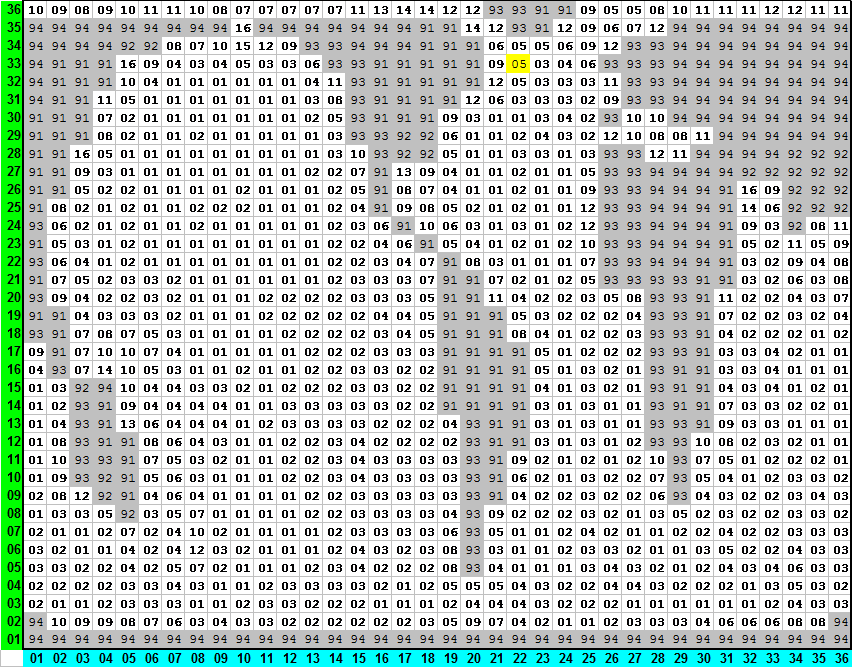
\includegraphics[width=0.8\textwidth]{ch3-ijgrid.png}\centering
\vspace{-0mm}
\caption{
\textbf{The  muffin grid for a modern \(36\times36\) ‘worjh2’ configuration.} Light blue numbers are the ‘i’ co-ordinates. Green numbers are the ‘j’ co-ordinates.
The depth of the ocean at any location is indicated by its ‘k’ value – a number between 1 and 16, with 16 being the surface layer of the ocean, and 1 the maximum possible depth anywhere.
Numbers > 90 (91, 92, 93, 94) and shaded grey are land (and specify the direction of run-off).
Location (22,33,08) is highlighted in yellow.
The longitude of the western edge of this particular modern ocean grid is at 260W, and the increments are 10 degrees. 
}
\label{fig:ch3-ijgrid}
\end{figure}

\begin{figure}
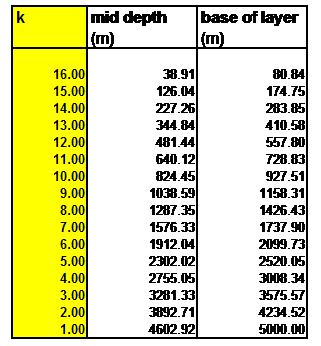
\includegraphics[width=0.4\textwidth]{ch3-kgrid.png}\centering
\vspace{-0mm}
\caption{\textbf{The muffin ocean vertical level definitions for a modern 16-level ocean grid.}}
\label{fig:ch3-kgrid}
\end{figure}

\hfill \break
\noindent\rule{4cm}{0.1mm}
\hfill \break

\noindent You are going to run a brief experiment in which you will be injecting a conservative ‘dye’ tracer into the ocean. The \textbf{BIOGEM} module has two tracers defined for this purpose – ‘blue’ and ‘red’. Open the \textit{user-config} file: \texttt{LAB\_2.colorinjection} and edit the parameter controlling the flux of red dye to read:

\vspace{-2mm}
\begin{verbatim}
bg_par_ocn_force_scale_val_48=1.0E12
\end{verbatim}
\vspace{-2mm}

\noindent which specifies a flux of \(1.0\times10^{12}\) ( \(mol yr^{-1}\)) rather than zero as given as the default in the example \textit{user-config} file\footnote{i.e. don't leave the value as zero ... otherwise you'll have no flux forcing applied and will not see anything happen ...}.

The \textit{base-config} you will be using is different from previously: \texttt{cgenie.eb\_go\_gs\_ac\_bg.worjh2.rb} – this specifies a 16 vertical levels ocean and also includes seasonality of solar insolation.

\hfill \break
\noindent\rule{4cm}{0.1mm}
\hfill \break

\noindent Run the model for … whatever, 20 years will do. Use the \textit{re-start} experiment that you have just downloaded to start from: 

\vspace{-2mm}
\begin{verbatim}
$ ./runmuffin.sh cgenie.eb_go_gs_ac_bg.worjh2.rb LABS
  LAB_2.colorinjection 20 LAB_2.SPIN
\end{verbatim}
\vspace{-2mm}

View the results – for instance how the red tracer distribution evolves with time – in the \textit{time-slice} files (full ocean/atmosphere) properties saved in the \textbf{netCDF} format (\texttt{.nc}) files). You can follow the progress of the dye (and hence diagnose the properties of ocean circulation in the model) by plotting vertical and/or horizontal slices that go through (or near) the cell location in which you inject the dye tracer in the 3D \textbf{netCDF} file. Note that \textbf{Panoply} appears to ‘count’ the ocean layers in the opposite direction to the way in which the ocean model is actually counting them – the correct definition is with ‘1’ being very deepest level possible (and as displayed in the figure).

You can also view the tracer distributions in terms of a water-column integrated tracer inventory (\textbf{netCDF} variable name: \texttt{ocn\_int\_colr}; long name: colr water-column integrated tracer inventory) in the 2D \textbf{netCDF} output. (See: \textit{Sabine et al.} [2004] for the use of water column integrals in the context of the distribution of anthropogenic \(CO_{2}\) uptake and storage.) Changes in tracer inventory with time can be tracked in the time-series file 

\vspace{-2mm}
\begin{verbatim}
biogem_series_ocn_colr.res.
\end{verbatim}
\vspace{-2mm}

You can also plot the overturning circulation from the 2D netCDF file – variable phys\_opsi == global overturning streamfunction, \texttt{phys\_opsia} == overturning in the Atlantic to provide a visualization of the large-scale ocean circulation that drives tracer movement.

Spend a little while altering the flux (\texttt{bg\_par\_ocn\_force\_scale\_val\_48}) and/or location (\texttt{bg\_par\_force\_point\_i}, \texttt{bg\_par\_force\_point\_j, bg\_par\_force\_point\_k}) of tracer input. Overall -- note how you can use numerical ‘tracers’ to help diagnose (and better understand) the circulation of the ocean.

\hfill \break
\noindent\rule{4cm}{0.1mm}
\hfill \break

\noindent An interesting (honest!) and illustrative exercise is to use the dye tracer to pick out the path taken by Mediterranean Intermediate Water. Despite the low resolution of the \textbf{muffin} ocean circulation model component and the highly restricted representation of the Mediterranean, the model does predict a salty Mediterranean as a consequence of P-E in this basin (and its catchments) being negative and this water makes its way out in the subsurface into the Atlantic.

Simply specify a dye injection somewhere in the Mediterranean (be careful with the restricted depth of the Mediterranean – if you inject too deeply (into the crust!) then you will not see anything (refer to the figure for the depth level (k) number of the maximum depth of the water column in each location), and it is better to inject it relatively close to the opening of the gateway (try some different locations and see which ones produce a reasonably instructive tracing of Mediterranean outflow). Run for e.g., 20 or 50 years (from the provided spin-up). Then:

\vspace{1mm}
\begin{enumerate}[noitemsep]
\vspace{1mm}
\item View the dye-tagged plume of Mediterranean Intermediate Water by plotting a lat-lon slice (from the 3D \textbf{netCDF} file). This will give you the depth of the plume. How does this compare with salinity observations (salinity observations and appropriate global datasets can be found on the web with a little patience)? You can also view the water-column integrated distribution (2D \textbf{netCDF}).
\vspace{1mm}
\item Try viewing the plume via a lat-depth slice. Refer to the figure to determine the ‘i’ value up the Atlantic that will just graze the edge of what passes for Spain at this low model resolution. Which direction does it head after exiting the Mediterranean? Is this ‘realistic’?
\end{enumerate}
\vspace{1mm}

%------------------------------------------------

\newpage

%------------------------------------------------

\section{Poking the climate beast}

Instead of adding a dye tracer, you could add fresh water to the ocean surface to assess the sensitivity of the Atlantic Meridional Overturning Circulation (AMOC) to collapse, in a classic ‘hosing’ experiment.

The \textit{user-config} file for this is called: \texttt{LAB.2.hosing}. The default (i,j) location of the flux input is the same (as the dye tracer), but now the injection at the surface (level: k=16). Note that the forcing of the salinity tracer is negative (freshwater = negative salinity compared to sea-water)!

To orientate you in freshwater forcing space: \texttt{bg\_par\_ocn\_force\_scale\_val\_2=-2.0E17} should be sufficient to make ‘stuff happen’ and quickly. BUT, this is a pretty extreme flux (see overleaf for a rough conversion between salinity forcing units (mol yr$^{-1}$) and fresh water flux (in m$^{3}$ s$^{-1}$ or Sv). Much more than this and the model may crash or at the very least, you’ll be left with a large freshwater pond in the North Atlantic … (See later (Section 1.6e) for some exciting discussion on units!)

To run the model for e.g., 20 years using the same restart:

\vspace{-2mm}
\begin{verbatim}
$ ./runmuffin.sh cgenie.eb_go_gs_ac_bg.worjh2.rb LABS
  LAB_2.hosing 20 LAB_2.SPIN
\end{verbatim}
\vspace{-2mm}

\noindent 20 years should be long enough to see a collapse start to occur, but you might want to run the model for longer (and it can be submitted as a job, of course). Running for longer will also allow you to have a smaller, less extreme (and maybe more realistic) freshwater input flux.

The most obvious property of the Earth system to follow is the Atlantic overturning strength (\texttt{biogem\_series\_misc\_opsi.res}). The AMOC stream-function (in \texttt{fields\_biogem\_2d.nc} 2-D time-slice \textbf{netCDF} results file, field: \texttt{phys\_opsia}) is also illustrative. You can also try and identify the salinity anomaly (see below) due to freshwater input in the 3D salinity tracer field.

There are also important impacts on surface air temperatures and maybe sea-ice extent (in \texttt{fields\_biogem\_2d.nc)}. Note the importance (sort of) of the AMOC in transporting heat to the N Atlantic region (the film the Day After Tomorrow was not entirely inaccurate in this particular respect). Be aware of the possibility of climate impacts far from the location of fresh water forcing. Look out for any significant-looking impacts on sea-ice extent, etc.

Note that as the model is running rather s l o w e r than in the snowball configuration, you might want to think carefully of making use of cluster queuing possibilities (i.e., running multiple experiments at once in the background).

\hfill \break
\noindent\rule{4cm}{0.1mm}
\hfill \break

\noindent To more easily assess some of these impacts (and for other sorts of analysis) it is possible to create an anomaly (difference) map in \textbf{Panoply}:

\vspace{1mm}
\begin{enumerate}[noitemsep]
\vspace{1mm}
\item  First open a dataset, e.g., \texttt{atm\_temp} (surface air temperature) in the 2D \textbf{netCDF} file. You can either double-click the variable name, or, with the variable name highlighted, click the ‘Create Plot’ icon.
\vspace{1mm}
\item Now, with the \texttt{atm\_temp} still selected (and the first plot window still open), click on the ‘Combine Plot’ icon. A dialogue box will appear and ask you to select a plot to combine the new one with. Make sure the name of your first plot window is selected/highlighted. Click ‘Combine’. OR, simply drag a second dataset into the plot window of the first dataset.
\vspace{1mm}
\item You now have a plot window that by default it is showing you the difference between two identical (in time) slices. The two different slices are labeled Array 1 (LH side) and Array 2 (RH side).
\end{enumerate}
\vspace{1mm}

Keep one array (Array 1) fixed to the initial (year 1 (centered on 0.5)) and vary the year in the second array (Array 2). Note that you can select in Panoply whether Array 1 – Array 2 is plotted, or Array 2 – Array 1, or various proportional or relative differences.

Note that you can switch off the auto-scaling feature (Always fit to data) and center the scale so that no change is white, with positive deviations = red and negative = blue by clicking on Center on 0 (an often used convention in climate field plotting).

Two example plots (using \textbf{Panoply}) are shown in Figure \ref{fig:ch3-amoc1} for the Atlantic basin, and Figure \ref{fig:ch3-amoc2} for the Pacific. 

\begin{figure}
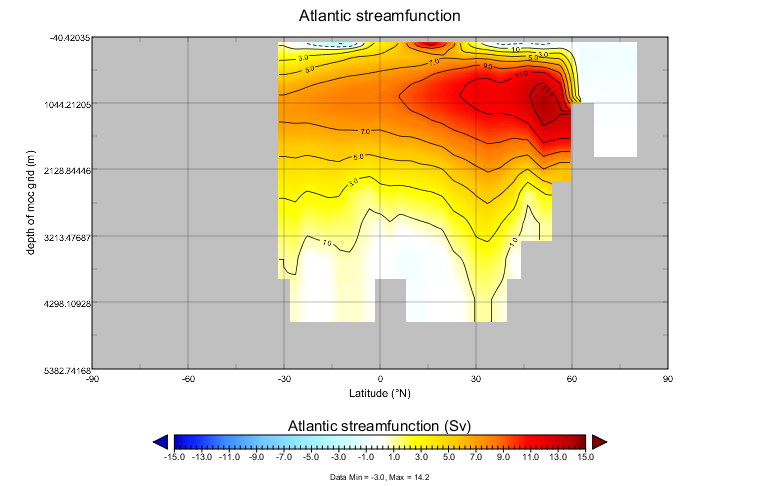
\includegraphics[width=0.6\textwidth]{ch3-amoc1.png}\centering
\vspace{-0mm}
\caption{Example plot of (normal/default modern) overturning streamfunction (2D \textbf{netCDF} file). (e.g., for Atlantic: \textbf{netCDF} parameter name: \texttt{phys\_opsia}, long-name: Atlantic streamfunction). Note that autoscaling has been turned off and the min and max plotting limits set manually. By convention, streamfunctions are plotted with their scale symmetrical around zero, giving red and ‘warm’ colors for positive value and clockwise overturning, and blues and ‘cold’ colors for negative values and anti-clockwise overturning. (The plot has been tart-ed up by overlaying solid contours plus contour labels.) It may be necessary in \textbf{Panoply} to re-orient (invert) the vertical grid.}
\label{fig:ch3-amoc1}
\end{figure}

\begin{figure}
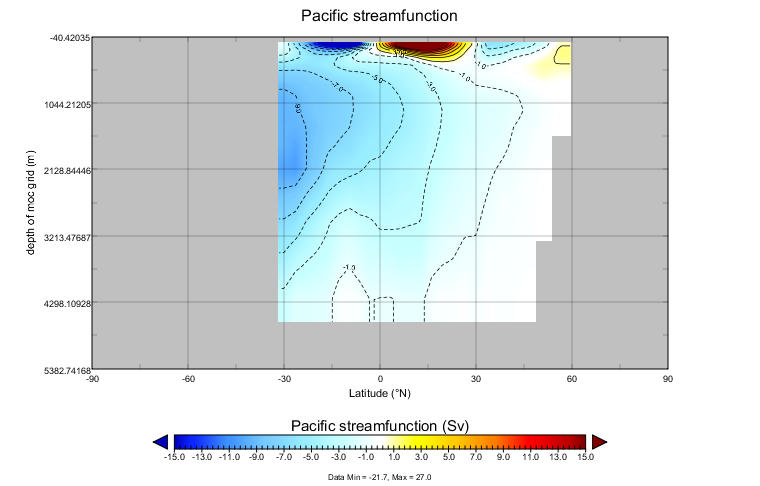
\includegraphics[width=0.6\textwidth]{ch3-amoc2.png}\centering
\vspace{-0mm}
\caption{Example plot of collapsed AMOC.}
\label{fig:ch3-amoc2}
\end{figure}

\hfill \break
\noindent\rule{4cm}{0.1mm}
\hfill \break

\noindent You can also plot ocean current fields which is sort-of fun and maybe even informative(!):

\vspace{1mm}
\begin{enumerate}[noitemsep]
\vspace{1mm}
\item  In the 3D \textbf{netCDF} file, the three components of ocean velocity are represented by the variables: ocean velocity – u (Eastwards), ocean velocity – v (Northwards), and ocean velocity – w (upwards). 2. Open up velocity – u. Chose ‘lon-lat’.
\vspace{1mm}
\item Select/highlight velocity – v. and click on the ‘Combine Plot’ icon (as per before).
\vspace{1mm}
\item Rather than a difference map, which is what you get by default, i.e., ‘Array 1 – Array 2’ – from the drop-down menu (next to the ‘Interpolate’ button) select ‘Vector Magnitude’.
\vspace{1mm}
\item You should have a color contoured (or not if you prefer plotting without contouring on) map of ocean current speed, with velocity vectors (direction and magnitude) overlain. You’ll need to re-scale the velocity vectors to properly see them – from the ‘Contours and Vectors’ tab – change the ‘Scale Length’ to e.g., 0.1. (On a \textbf{Mac}, look under the ‘Vectors’ tab for a ‘Reference Value’ to something like 0.1.)  When fresh-water hosing – look out for impacts on the N. Atlantic current system associated with the AMOC.
\vspace{1mm}
\item You can repeat this for deeper depth levels in the ocean – e.g., between about 1500 and 2000 m is a good place to go looking for the Western boundary current (and AMOC return) in the model (such as it exists at this low resolution) but you’ll need to re-scale the velocity vectors again (e.g., to 0.01 to less).
\end{enumerate}
\vspace{1mm}

\noindent An example plot (using \textbf{Panoply} for visualizing surface ocean current fields) is given in Figure \ref{fig:ch3-currents1}. 

\begin{figure}
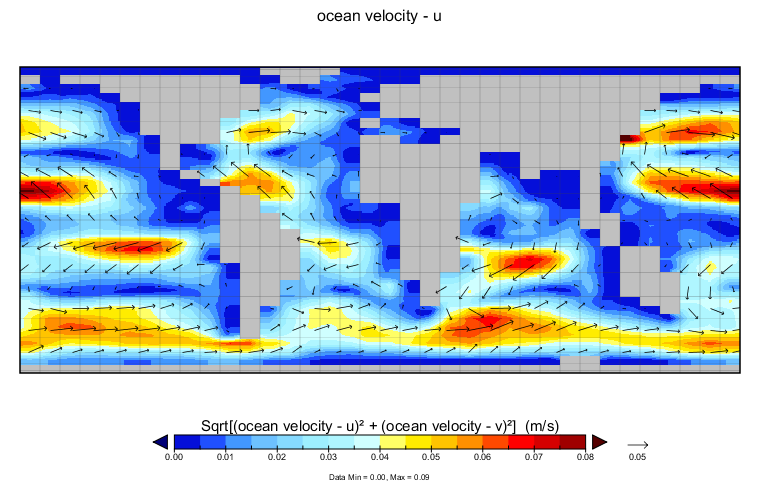
\includegraphics[width=0.6\textwidth]{ch3-currents1.png}\centering
\vspace{-0mm}
\caption{Example plot of (normal/default modern) ocean current fields (3D netCDF file). Again scaling has been set manually to create an easy-to-interpret axis scale. On the left is the surface field, and on the right an intermediate depth (illustrating what approximates the Deep Western Boundary current in the model in the Atlantic).}
\label{fig:ch3-currents1}
\end{figure}

\hfill \break
\noindent\rule{4cm}{0.1mm}
\hfill \break

\noindent Finally, a brief note on units ... the freshwater forcing is implemented as negative salinity, just to really screw with your mind. The generic internal \textbf{muffin} model units for the forcing end up as \(PSU kg^{-1} yr^{-1}\). Which sort of does not make much sense ...

Start, by thinking of a value of \texttt{bg\_par\_ocn\_force\_scale\_val\_2} of \(-34.9\) as equivalent to taking all the salt out of \(1 kg\) of freshwater (since the mean global salinity is \(34.9 PSU\)). Or equivalently, since the ocean volume is fixed, an applied forcing value of \(-34.9\) is equivalent to adding \(1 kg\) of freshwater to a (surface) box. So, a value of \texttt{bg\_par\_ocn\_force\_scale\_val\_2} of \(-3.49\times10^{4}\) (\(-3.49E04)\) would be a flux of \(1 m^{3} yr^{-1}\) (\(1000 kg m^{-3}\)) of freshwater.

So, in the example earlier (\texttt{bg\_par\_ocn\_force\_scale\_val\_2=-1.0E18}), the freshwater flux is \(1.0\times10^{18}/3.49\times10^{4} = 2.8653\times10^{13} m^{3} yr^{-1}\).

The literature invariably gives freshwater fluxes in units of \(Sv\) (\(10^{6} m^{3} s^{-1}\)). So in the example, the freshwater flux is: \(9.0797\times10^{5} m^{3} s^{-1}\) (\(365.25\times24\times3600 = 31557600 s yr^{-1}\)). Or \(0.9 Sv\). Read the literature … but generally, fluxes of ca. \(0.05 Sv\) and larger (and to quite specific places) are applied in models to induce an AMOC collapse.

%------------------------------------------------

\newpage

%------------------------------------------------

\section{Further ideas}

%------------------------------------------------

\subsection{Hosing investigations}

What is the largest freshwater flux that can be sustained without ‘collapsing’ the AMOC? Is there a ‘threshold’ (‘tipping point’) of freshwater input, beyond which the AMOC rapidly decreases in strength?

Is the precise location of the freshwater input important (i.e., try tipping it in somewhere else)? What would you expect to see in the paleo (e.g., ice core) record of both hemispheres if such a shutdown occurred in the past?

Are any other major regions of deep water formation (where are they) sensitive to freshwater perturbation and what are the consequences (could it happen in the future)?

%------------------------------------------------

\subsection{‘Anti-hosing’ investigations}

There are questions concerning past changes in the AMOC as to whether it is ‘pushed’ or ‘pulled’. i.e., if the AMOC shoals in depth and/or weakens, is it because its production has weakened, or as Antarctic Bottom water (AABW) strengthened and ‘pushed’ it out of the way (to shallower depths)?

What you might try then is to inject salt in the Southern Ocean as opposed to fresh water in the North Atlantic. All you need do is pick an appropriate grid point (this is worth thinking about carefully and maybe testing different locations) and rather than giving the parameter \texttt{bg\_par\_ocn\_force\_scale\_val\_2} a negative value, you give it a positive one. (Start by trying similar magnitudes of value as before and see what happens.) 

\textbf{Is the AMOC (for the same magnitude of forcing) more sensitive to being ‘pushed’ or ‘pulled’?} (Obviously the answer will very much depend on where the perturbations are being applied.)

%------------------------------------------------

\subsection{Response to transient warming}

A current concern regarding anthropogenic climate change is the ocean circulation (and marine ecological and biogeochemical) response to a strong warming of the surface, as rapid surface warming is assumed (and demonstrated in models) to result in surface stratification of the ocean, likely restricting the nutrient supply to phytoplankton and reducing ventilation of the ocean interior with dissolved oxygen.

You can explore the transient response of ocean circulation to warming by simply adjusting the radiative forcing parameter as per used in the snowball Earth experiments: \texttt{ea\_radfor\_scl\_co2}. By default in the modern continental configuration, this has a value of 1.0, corresponding to 278 ppm atmospheric \(CO_{2}\). A value of 2.0 would reflect warming equivalent to 556 ppm \(CO_{2}\). And 3.0 more like an end-of-the-century warming. Note that you are applying the warming instantaneously by manipulating the climate system in this way and hence the changes will be more extreme than those occurring over the time-scale of this century. Also note that a cooling could be applied instead. A \textit{user-config} – \texttt{LAB\_2.EXAMPLE} – is provided as a template for these experiments.

Potentially interesting properties of the Earth system to look at include sea-ice extent and AMOC strength (in the ASCII time-series files), and the overturning streamfunction and sea-ice extent in the 2-D \textbf{netCDF} output.

\textbf{How much radiative forcing is required to collapse the AMOC? What atmospheric \(CO_{2}\) value does this approximately correspond to?
}

%------------------------------------------------

\subsection{Ventilation age tracers}

\textbf{muffin} has the capability to employ/simulate a ventilation age tracer\footnote{Under the '\textit{screw with and/or diagnose the climate system}' HOW-DO -- see '\textit{Add a water mass age tracer}' (and the 'easy'/automatic method described towards the end of that section).} -- a numerical tracer in the ocean that tracks the time since a parcel of water last 'saw' the surface. To do this, requires both 'red' and 'blue' numerical tracers to be selected.  \textbf{muffin} can then be directly to automatically apply the forcings necessary to each tracer in order to simulate water mass ventilation age.

Provided is an additional \textit{user-config} file: \texttt{muffin.worjh2.NONE\_colage.EXAMPLE}.

A new \textit{re-start} experiment is provided called \texttt{muffin.worjh2.NONE\_colage.SPIN} and which can be downloaded as per before:

\vspace{-1mm}
\small
\begin{verbatim}
$ wget http://www.seao2.info/cgenie_output/muffin.worjh2.NONE_colage.SPIN.tar.gz
\end{verbatim}
\normalsize
\vspace{-1mm}

\noindent and unpacked, as before, by:

\vspace{-1mm}
\begin{verbatim}
$ tar xfzv muffin.worjh2.NONE_colage.SPIN.tar.gz
\end{verbatim}
\vspace{-1mm}

\noindent (Remember: you should be in the \texttt{cgenie\_output} directory when you do this.)

To run (e.g. for 10 years), following on from its \textit{re-start} experiment:

\vspace{-1mm}
\small
\begin{verbatim}
$ ./runmuffin.sh cgenie.eb_go_gs_ac_bg.worjh2.rb LABS muffin.worjh2.NONE_colage.EXAMPLE
    10 muffin.worjh2.NONE_colage.SPIN
\end{verbatim}
\normalsize
\vspace{-1mm}

\noindent (all on one line)

In the 3D netCDF output file -- \texttt{misc\_col\_Dage} is the output variable that is the calculated ventilation age.

First -- explore the distribution of water mass age and think about the physical ocean circulations reasons for this. Are all the modelled distributions reasonable? Are there indicators of facets of the simulated circulation that are not particularly realistic? Try plotting both lon-lat and lat-depth slices through the ocean.

Secondly -- you could additionally combine this experiment configuration with fresh water hosing, or a prescribed radiative forcing (and warming), and explore how ocean ventilation responds as ocean circulation changes. (You'll need to create for yourself a new \textit{forcing} directory and set of files that now combines both color tracers AND a freshwater flux.)

%----------------------------------------------------------------------------------------
%       CHAPTER 4
%----------------------------------------------------------------------------------------

\cleardoublepage

\chapterimage{Jay-Matternes---EOCENE.jpg} % Chapter heading image

\chapter{Climates of Past Worlds}

\hfill \break

\vspace{12mm}

\noindent This Chapter comprises 2 different exercises, both employing 'realistic' reconstructions of past continental configuration and climate and designed to explore some of the key controls on global surface climate as well as the spatial pattern of surface temperatures.

The two exercises concern the late Cretaceous and early Eocene climate states, and are somewhat interchangeable.

\section*{Background reading (Cretaceous climate)}
\begin{itemize}
\item Barron, E.: A warm equable Cretaceous: the nature of the problem, Earth-Science Reviews 19, 305–338, 1983.
\item Bice, K. L., and R. D. Norris, Possible Atmospheric \(CO_{2}\) extremes of the middle Cretaceous (late Albian-Turonian), Paleoceanography 17, doi: 10.1029/2002PA000778, 2002.
\item Bice, K. L., B. T. Huber, and R. D. Norris, Extreme polar warmth during the Cretaceous greenhouse?: Paradox of the Late Turonian \(d18O\) record at DSDP Site 511, Paleoceanography 18, doi: 10.1029/2002PA000848, 2003.
\item Bice, K. L., D. Birgel, P. A. Meyers, K. A. Dahl, K. Hinrichs, and R. D. Norris, A multiple proxy and model study of Cretaceous upper ocean temperatures and atmospheric \(CO_{2}\) concentrations, Paleoceanography 21, PA2002, doi:10.1029/2005PA001203, 2006.
\item Donnadieu, Y., et al., Modelling the primary control of paleogeography on Cretaceous climate, Earth and Planetary Science Letters 248, 426–437, 2006.
\item Huber, B. T., Norris, R. D., and MacLeod, K. G.: Deep-sea paleotemperature record of extreme warmth during the Cretaceous, Geology 30, 123–126, 2002.
\item Hunter, S. J., et al., Modelling Maastrichtian climate: investigating the role of geography, atmospheric \(CO_{2}\) and vegetation, Clim. Past Discuss. 4, 981–1019, 2008.
\item Jenkyns, H. C., Forster, A., Schouten, S., and Sinninghe Damste, J. S.: High temperatures in the Late Cretaceous Arctic Ocean, Nature 432, 888–892, 2004.
\end{itemize}

\section*{Background reading (Eocene climate)}
\begin{itemize}
\item Dunkley Jones, T., D.L. Lunt, D.N. Schmidt, A. Ridgwell, A. Sluijs, P.J. Valdes, and M. Maslin, Climate model and proxy data constraints on ocean warming across the Paleocene-Eocene Thermal Maximum, Earth-Science Reviews 125 123–145 (2013).
\item Lunt, D. J., Dunkley Jones, T., Heinemann, M., Huber, M., LeGrande, A., Winguth, A., Loptson, C., Marotzke, J., Roberts, C. D., Tindall, J., Valdes, P., and Winguth, C.: A model–data comparison for a multi-model ensemble of early Eocene atmosphere–ocean simulations: EoMIP, Clim. Past, 8, 1717-1736, doi:10.5194/cp-8-1717-2012, 2012.
\end{itemize}

%------------------------------------------------

\newpage

%------------------------------------------------

\section*{READ.ME}

You will need to download new \textit{restart} files for this Chapter (both 10,000 year spin-ups). These are:

\vspace{2mm}
\begin{enumerate}[noitemsep]
\item[\textbf{Cretaceous:}]
\begin{verbatim}
$ wget http://www.seao2.info/cgenie/labs/AWI.2017/LAB_5.SPIN.tar.gz
\end{verbatim}
\item[\textbf{Eocene:}]
\begin{verbatim}
$ wget http://www.seao2.info/cgenie/labs/AWI.2017/LAB\_5b.SPIN.tar.gz
\end{verbatim}
\end{enumerate}
\vspace{2mm}

Extract the results in the usual way and in the usual place ... and return to \texttt{genie-main}.

%------------------------------------------------

\newpage

%------------------------------------------------

\section{The climate of the Cretaceous}

A previously spun-up state of Maastrichtian climate with \textbf{cGENIE.muffin} in a ca. 70 Ma configuration\footnote{Note that for speed, no carbon cycle is selected in this configuration.} (\texttt{LAB\_5.SPIN}) is provided as a starting point. A \textit{user-config} (\texttt{LAB\_5.EXAMPLE}) that continues on this climate state is run:
\begin{verbatim}
$ ./runmuffin.sh cgenie.eb_go_gs_ac_bg.p0067f.NONE LABS 
 LAB_5.EXAMPLE 10 LAB_5.SPIN 
\end{verbatim}

Your task now is ... ‘simple’: Account for the Cretaceous reduced Equator-to-pole surface temperature gradient (compared to modern), particularly the apparently much warmer poles. Different data-based time-slices (including the Maastrichtian) are provided in \textit{Huber et al.} [2002], although the low latitude \(\delta^{18}O\) based temperatures are now not considered reliable. \textit{Jenkyns et al.} [2004] contains high latitude (Arctic) data for the Maastrichtian. There are proxy-derived latitudinal temperature gradients and model-data studies for earlier in the Cretaceous – the problem is essentially the same.

The 2-D NetCDF results file contains the surface air temperature field (and sea-ice cover, if any). The 3-D NetCDF results file contains fields for ocean temperatures (and salinity). Both contain continental configuration and ocean bathymetry.

\textbf{Panoply} will plot the zonal average for you (as used in model-data comparisons – e.g., see Bice and Norris [2002]) – in the Array(s) tab, the Plot can be set to Zonal Averages rather than Map. You can get a smooth curve by selecting Interpolate. Remember you can set (and fix) scales rather than let Panoply auto-scale continually.

The following ‘controls’ over the climate system are provided to you in the form of a list of parameters at the bottom of the \texttt{LAB\_5.EXAMPLE} \textit{user-config} file for editing:

\small\begin{verbatim}
# --- MISC -----------------------------------------------
#
# === ATMOSPHERE ===
# \(CO_{2}\) radiative forcing scaling factor [DEFAULT = 4.0]
ea_radfor_scl_co2=4.0
# CH4 radiative forcing scaling factor [DEFAULT = 1.0]
ea_radfor_scl_ch4=1.0
# Equator-to-pole different in planetary albedo [DEFAULT = 0.260]
ea_albedop_amp=0.260
# Baseline planetary albedo [DEFAULT = 0.200]
ea_albedop_offs=0.200
# atmospheric diffusivity of temperature (horizontal) [DEFAULT = 5.0e6]
ea_12=5.0e6
# === OCEAN ===
# ocean diffusivity of temperature + salinity (horizontal) [DEFAULT = 1494.4]
go_14=1494.4
# scaling for wind stress (set values of both identical) [DEFAULT = 1.531]
go_13=1.531
ea_11=1.531
\end{verbatim}\normalsize

Most of these parameters are associated with the radiative forcing of climate or atmospheric transports. The most useful ones are likely to be:

\begin{itemize}[noitemsep]

\item[\textbf{(i)}] The line: 
\begin{verbatim}
ea_radfor_scl_co2=4.0
\end{verbatim}
which specifies a radiative forcing of climate by \(CO_{2}\) equivalent to \(4\) times modern \(CO_{2}\) (i.e., \(4\times278 ppm = 1112 ppm\)) as per before (e.g. snowball Earth experiments).
\\The line: 
\begin{verbatim}
ea_radfor_scl_ch4=1.0
\end{verbatim}
specifies a radiative forcing of climate by \(CH_{4}\) equivalent to \(1\) times modern \(CH_{4}\) (i.e., \(1\times700 ppb\)).\footnote{But effectively, this is going to do exactly the same as changing radiative forcing due to \(CO_{2}\).}

\item[\textbf{(ii)}] cGENIE, as configured here, does not have a land surface scheme (no snow cover) nor clouds nor ice sheets, so a planetary albedo is prescribed (see Figure 4.1). This varies with latitude and is parameterized after a fully coupled GCM simulation. There is a parameter which controls how the albedo varies as a function of latitude, which can be adjusted: 
\begin{verbatim}
ea_albedop_amp=0.260
\end{verbatim}
However, if you vary this, why are you doing it? (What is the physical justification for giving the poles a higher or lower albedo relative to the Equator?)
There is also a parameter that sets the baseline (minimum) albedo: 
\begin{verbatim}
ea_albedop_offs=0.200
\end{verbatim}
i.e., albedo is primarily a sum of the baseline value plus the Equator-to-pole slope (times the latitude).

\item[\textbf{(iii)}] The diffusivity of heat in the atmosphere (since it is a simple 2-D atmospheric model, with no atmospheric circulation, the atmosphere is made ‘diffusive’ to help capture heat and moisture transport) is: 
\begin{verbatim}
ea_12=5.0e6
\end{verbatim}
Note the maximum value the model can cope with is ca. \(1.0E7\).

\end{itemize}

\begin{figure}
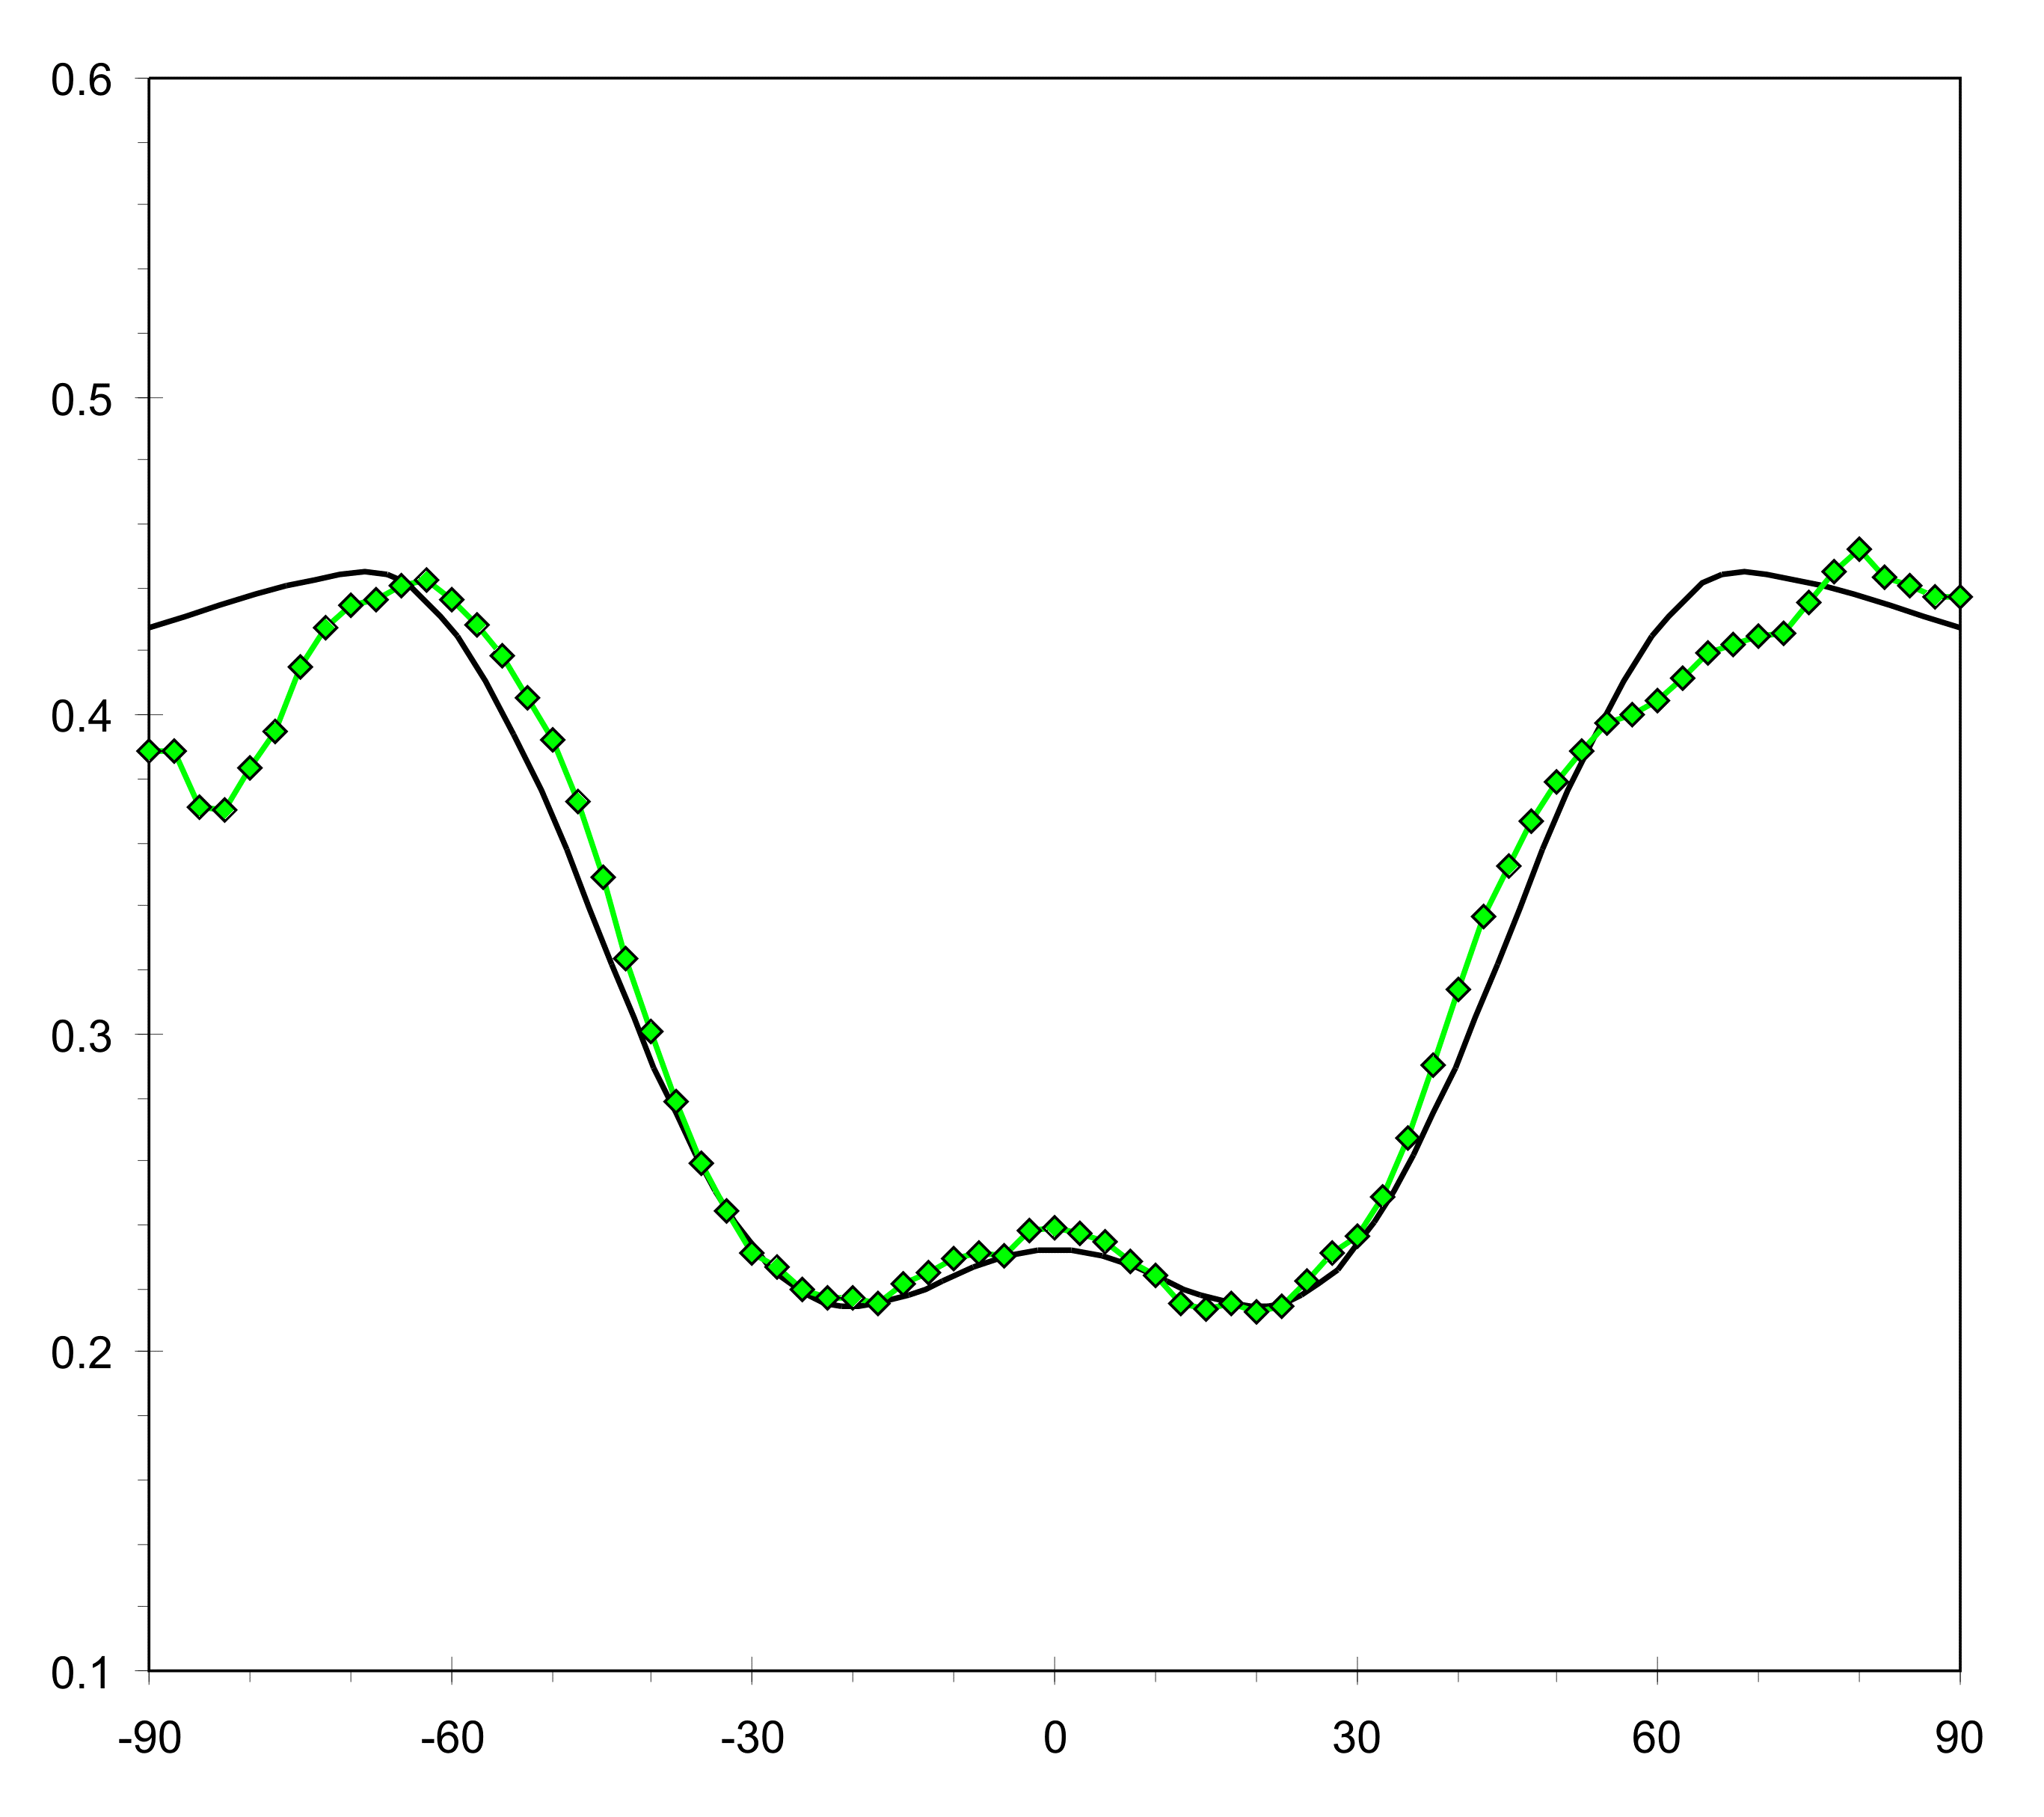
\includegraphics[width=0.6\textwidth]{tmp-albedo.png}\centering
\vspace{-6mm}
\caption{Prescribed planetary albedo. 
The latitudinal (from 90$^{\circ}$S (-90$^{\circ}$N) on the left, to 90$^{\circ}$N on the right) profile of planetary albedo as calculated in a fully coupled GCM is given in green, and the cGENIE ‘fit’ in black.}
\label{fig:tmp-albedo}
\end{figure}

\vspace{1mm}
\noindent\rule{4cm}{0.1mm}
\vspace{2mm}

\noindent Run the model for however long you think is ‘necessary’ (/justified). The surface climate will approach equilibrium ‘relatively’ quickly. Deep ocean temperatures will typically take thousands of years to fully adjust ... You can assess how the model approaches equilibrium most easily from the atmospheric temperature time-series results file, and from the ocean temperature time-series results file (allowing to you to contrast surface and whole ocean temperature changes).

\vspace{1mm}
\noindent\rule{4cm}{0.1mm}
\vspace{2mm}

\noindent You can also try tracing and analyzing the patterns of ocean circulation in the Cretaceous world, in the same way as you did for the modern climate system. And in fact, it would be a useful exercise to directly compare your previous modern results vs. Cretaceous results, or even better, carry out a set of paired experiments (e.g., similar locations and fluxes of dye injection) for both modern and Cretaceous. (Note that if you do this and swap back and forth between modern and Cretaceous configurations, you cannot submit straight away to the cluster but must first briefly run the experiment at the command line in order that cGENIE is compiled into the new continental configuration.)

A new \textit{user-config} (\texttt{LAB\_5.colorinjection}) that continues on from this climate state, can be run: 
\begin{verbatim}
$ ./runmuffin.sh cgenie.eb_go_gs_ac_bg.p0067f.rb LABS 
 LAB_5.colorinjection 10 LAB_5.SPIN 
\end{verbatim}
(Also note that the \textit{base-config} is different as it now includes the definition of 2 dye tracers.)

The default locations for the dye release are set different compared to in the modern configuration. BUT, the default location is not necessarily ideal / particularly revealing … so you’ll need to look count grid cells West-to-East (the i direction) and from South to North (the j direction) in order to determine a more suitable location for tracing circulation.

By means of dye tracing, looking at the (global only) overturning stream-function, and/or temperature and salinity (and density) profiles, see if you can identify where in the Cretaceous ocean deep water forms in the model. AND, more importantly, think about WHY does it form where it does?

Also: what about surface ocean circulation and gyres? Are these located where you would expect (e.g. based on your understanding of modern ocean circulation). Plot velocity vectors to help, and/or refer to the Barotropic streamfunction output in the 2D netCDF file.

%------------------------------------------------
%
\newpage

%------------------------------------------------

\section{The climate of the early Eocene}

A previously spun-up state of early Eocene climate with cGENIE in a ca. 56 Ma configuration (\texttt{LAB\_5b.SPIN}) is provided as a starting point. A user-config (\texttt{LAB\_5b.EXAMPLE}) that continues on this climate state is run: 
\begin{verbatim}
$ ./runmuffin.sh cgenie.eb_go_gs_ac_bg.p0055c.NONE LABS 
 LAB_5b.EXAMPLE 10 LAB_5b.SPIN 
\end{verbatim}
(Note that once again, for speed, no carbon cycle is selected in this configuration.)
Again, as per for the late Cretaceous configuration, a configuration that includes the ocean dye (color) tracers is also provided. The corresponding user-config (\texttt{LAB\_5b.colorinjection}) that continues on this climate state can be run as follows: 
\begin{verbatim}
$ ./runmuffin.sh cgenie.eb_go_gs_ac_bg.p0055c.rb LABS 
 LAB_5b.colorinjection 10 LAB_5b.SPIN 
\end{verbatim}
 
\vspace{1mm}
\noindent\rule{4cm}{0.1mm}
\vspace{2mm}

\noindent What to ‘do’ with this? Again – start by tracing and analyzing the patterns of ocean circulation in the Eocene world, as per how you did for the modern and Cretaceous system. Where does deep water form in the Eocene? Is the surface ocean circulation as expected?
Can you see any patterns emerging? At least in model world – what seems to be dictating the locations of deep water formation? Does overturning and/or surface circulation appear to significantly vary as a function of continental configuration or radiative forcing? If not, why not?

\vspace{1mm}
\noindent\rule{4cm}{0.1mm}
\vspace{2mm}

\noindent But how do you know how close, or not, the model climate is to ‘reality’? 
Available from the website, on the LH side of the page under ‘got data?’ at the bottom (item (7)), are 2 netCDF files containing proxy sea surface temperature (SST) data re-gridded to the cGENIE model grid. One is for pre-PETM SSTs, and one for peak PETM SSTs. (The data are from Dunkley Jones et al. [2013].)

These netCDF files can be opened and visualized in exactly the same way in exactly the same way as per the cGENIE output files. You’ll see a few (there are not many!) data points, in a sea of grey (which stands for ‘no value’). (Note that it is best to turn data interpolation OFF.)

More useful … is that the data distribution can be combined with the model ocean temperature output field, in a difference map (see earlier for notes on creating difference maps). You can thus visualize the pattern of model-data mismatch. (Note you might want to hit ‘Fit to data’ to autoscale the plot, or simply pick and manually enter a +/- limit for the data plotting, perhaps ensuring it is symmetrical about zero such that red anomalies could represent proxy SST values higher than in the model, and blue point data being lower than in the model.)

Furthermore, in the Arrays tab, you can switch to a Zonal Average view rather than a Map view (...it is probably easier to visualize the model-data misfit in this way.)

\vspace{1mm}
\noindent\rule{4cm}{0.1mm}
\vspace{2mm}

\noindent So, starting with the pre-PETM data and given model configuration, make some assessment of how the model fits the data (or not). What might be the reason for the misfit? You might test adding, and adjusting, some of the parameter values controlling surface SST from the Cretaceous climate exercise. Can you reduce the model-data misfit?

\vspace{1mm}
\noindent\rule{4cm}{0.1mm}
\vspace{2mm}

\noindent Finally, the PETM SST data given in the 2nd netCDF file are from the peak of the PETM. The ocean is rather warmer as compared to just prior to the PETM. Your task is to determine (either using the default model configuration, or your adjusted configuration) much radiative forcing (parameter \texttt{ea\_radfor\_scl\_co2}) and hence \(CO_{2}\) is required to explain this warming? 

%----------------------------------------------------------------------------------------
%       CHAPTER 4
%----------------------------------------------------------------------------------------

\cleardoublepage

\chapterimage{middle_earth.png} % Chapter heading image

\chapter{Alternative Oceans}

\hfill \break

\noindent Fake (alternative) Worlds are a useful tool for developing a general understanding of how climate (and ocean circulation) and global biogeochemical cycles operate. Different model resolutions and continental configurations can be generate and run to test specific hypotheses about the role and sensitivity of different elements in Earth system to emergent patterns of climate (and biogeochemical cycling). Ensembles of differing Worlds can also be utilized to more generalize understanding as well as in a fishing expedition of new or unexpected phenomena and system behaviours.

This Chapter will take you through the generation and exploration (analysis) of fake (alternative) Worlds. 

%------------------------------------------------

\newpage

%------------------------------------------------
%
\section{Generating fake Worlds}

%------------------------------------------------

\vspace{1mm}
\noindent\rule{4cm}{0.5pt}
\vspace{2mm}

\noindent\textcolor{red}{TO COME ...}

\vspace{1mm}
\noindent\rule{4cm}{0.5pt}
\vspace{2mm}

%------------------------------------------------

\newpage

%------------------------------------------------
%
\section{Understanding ocean circulation}

%------------------------------------------------

What follows, outlines different ways of visualizing and quantifying ocean circulation in \textbf{muffin}, and coming to a model-empirical understanding of ocean circulation controls.

%------------------------------------------------

\subsection{Model investigation over-view}

In restricting model-based experiments and derived understanding to   the modern continental configuration (and climate) in \textbf{muffin}, you'd be unlikely to come to any particularly deep or fundamental insights into ocean circulation controls in general. In any case, the modern and future (and recent glacial past) ocean circulation states and dynamics has been picked at endlessly by 1000s of researchers, writing 100,000s of  publications ... and yet still we do not fully understand modern ocean circulation, let along that at the last glacial. 

A better (more fun) approach is to generalise the problem and consider fundamentally different configurations of ocean basins and climate. This is what you will be doing. But first, some potted advice:

\vspace{2mm}
\begin{itemize}[noitemsep]
\vspace{1mm}
\item Try and define a hypothesis, or hypotheses, to pursue and test. These need only be very rough at the outset -- you'll likely find that you get new ideas and can either refine your original hypotheses, or come up with new ones, as you start to play with the model and see what is feasible and not feasible in terms of analysis.
\vspace{1mm}
\item Create a plan of study -- what sort of experiments, now many, how are they going to be analysed, how do they all fit together in addressing the overarching hypotheses? Again -- it is very likely that your plan will evolve, but try and start out with something to guide you rather than wandering randomly in model world ...
\vspace{1mm}
\item For creating and an using different worlds -- create a list or table of the configurations to be explored, and summarize what you are finding. It might be helpful to plan out on paper first, some of the main continental configurations you need to create and then test in the model. (Again, this will evolve.)
\vspace{1mm}
\item Once you have some sort of idea what are are going to do -- plan the work. This is important because to run the model to steady state is not trivial. Perhaps plan on having to run the model for 5,000 years\footnote{Even so, you should try running the model much longer to be confident that 5,000 years is OK (and sufficiently close to final equilibrium).} in order to achieve a fully spun up ocean circulation state. You might get away with shorter runs, but know in advance what sort of error this would induce and is it 'important'? Once you have a list and know how long each might take, you can plan out when they will be run on the cluster (presumably on the queue) and when the results will be analysed. Note that it is a virtual certainty that once you have analysed the results of the first set of experiments, you will want something different (and will then need to revise the plana and list of experiments and analysis etc.).
\end{itemize}
\vspace{2mm}

\noindent Overall -- scientific investigations with simplified (and relatively fast) Earth system models tends to become a somewhat iterative undertaking and can involve significant trail-and-error. (This is healthy and to be expected and even enjoyed!) Rarely, can you devise at the outset, a single run or set of experiments, and it turns out this is completely sufficient. If you do not see something you do not understand in the results of the initial model experiments, you are either God (e.g. the Spaghetti Monster or Invisible Pink Unicorn), or not doing it properly. Expect to see things that interest you and lead you off on a tangent (hopefully -- this is how research should be).

Finally -- \uline{note} that in swapping between different continental configurations, \textbf{muffin} currently requires the model executable to be  re-compiled.\footnote{Note that if the \textit{base-config} is the same as the previous experiment, but you have changed a parameter value (in the \textit{user-config}), you do not need to re-compile.} This ... cannot happen on the compute nodes of the cluster if you submit an experiment using a different \textit{base-config}. When changing to a new \textit{base-config}: \uline{first}, run the model briefly interactively (i.e. at the command line). Once it has compiled (and started running), the experiment can be killed (\textsf{ctrl-c}) and now it is good to submit to the queue as a job. In any case, in utilizing a new configuration that you may never have used before, it is good practice to test it first (e.g. watch it run for a short period).

%------------------------------------------------

\subsection{Deep-water formation (\& baroclinic circulation)}

The first investigation is to investigate the controls on the strength and large-scale structure of ocean circulation, particularly in terms of the global meridional overturning circulation (MOC), and associated with this -- the primary sites of deep-water formation.

There are presumably 2 key controls to this:

\vspace{2mm}
\begin{enumerate}
\item \textbf{Temperature.}
\\This is presumably mostly a function of latitude (i.e. the further North or South, the more suitable the site will tend to be for deep-water formation) and to some extent season. There will also be an influence of the prescribed planetary albedo (which includes the effect of clouds) as well as of sea-ice (if it exists).
\vspace{2mm}
\item \textbf{Salinity.}
\\This will generally be controlled by P-minus-E -- the balance between precipitation to the ocean surface as well as fresh-water run-off form the continents, vs. evaporation from the ocean surface. Sea-ice may also be a key factor, in e.g. leading to the (seasonal) rejection of dense salty brine (and removal of freshwater to the forming ice).
\end{enumerate}
\vspace{2mm}

In turn, this suggests two sets of 'knobs' in the model that influence the patterns and magnitude of temperature and salinity across the ocean surface:

\vspace{1mm}
\begin{enumerate}
\vspace{1mm}
\item \textbf{Continental Configuration.}
\\The configuration of the continents and ocean basins will dictate the shape and location of the highest latitude ocean regions -- presumably the locations where on average, deep-water formation will occur (and hence forming the downwards/sinking limb of the MOC).
\\The relevant model 'knob' is hence how the position and orientation of continental blocks is configured on the surface of the Earth. This (creating or changing the continental configuration used by \textbf{muffin}) can all done using the \textbf{MATLAB} \textbf{muffingen} program.
\vspace{1mm}
\item \textbf{Global Climate.}
\\The mean and climate as well as the zonal temperature gradients, together with whether or not sea-ice forms (and how much), will modulate both temperature and salinity patterns at the ocean surface.
\\The model knobs here are primarily:
\begin{enumerate}
\item Atmospheric \(pCO_{2}\), or in the absence of an explicit carbon cycle, a prescribed radiative forcing:
\vspace{-2pt}\begin{verbatim}
ea_radfor_scl_co2=1.0
\end{verbatim}\vspace{-2pt}
which here, specifies \(\times1\) \(CO_{2}\) equivalent radiative forcing.
\item One could also adjust the value of the solar constant (here, given with its modern/present-day default value):
\vspace{-2pt}\begin{verbatim}
ma_genie_solar_constant=1368.0
\end{verbatim}\vspace{-2pt}
which has a subtly different effect form changing \(CO_{2}\) radiative forcing, as radiative forcing has a relatively spatially uniform impact, whereas changing the solar constant has a disproportionate impact towards the Equator (where the incident solar shortwave radiation is the greatest). So changing the solar constant is likely to impact the pole-to-Equator temperature gradient. e.g. see: Lunt, D. J., A. Ridgwell, P. J. Valdes, and A. Seale, Sunshade World.: a fully coupled GCM evaluation of the climatic impacts of geoengineering, GRL 35, L12710, doi:10.1029/2008GL033674 (2008).
\item One could also adjust the planetary albedo, particularly in respect of looking to modify the pole-to-Equator temperature. In the \textbf{muffingen} created configurations, there is an explicit 1D file specifying the zonal (with latitude) planetary albedo profile:
\vspace{-2pt}\begin{verbatim}
xxxxxxxx.albd.dat
\end{verbatim}\vspace{-2pt}
where \texttt{xxxxxxxx} is the 8-character name of the \textbf{muffingen} created World. It would be a simple matter of editing the values in the file (between the range of 0.0 and 1.0, for  perfectly absorbing, and perfectly reflective, respectively).\footnote{Best to make a copy of the original file before you modify it.} Note that the file data order is North-to-South (going from top to bottom in the file).
\end{enumerate}
\end{enumerate}
\vspace{2mm}

%------------------------------------------------

\subsection{Gateways and barotropic flow}

The overarching question in the context of ocean gateways and barotropic flow, is a little harder to define succinctly; it has to do with the details of the degree of alignment (or not) of the prevailing wind (stress)
with  gateways, and the degree to which this give rise to strong zonal ocean flow. A good and obvious modern example is the existence of the Drake Passage, between the northern tip of the Antarctic Peninsular, and the southern tip of Souther America, how this aligns with the prevailing Westerlies in the Southern Hemisphere, and hence the nature and strength of the ACC (Antarctic Circumpolar Current).

So the question naturally arises: how misaligned does a gateway have to be relative to the prevailing wind stress maximum, before the circumpolar (or circum-equatorial) flow ceases. What about having multiple gateways and their relative alignment, including what happens if one gateway is aligned with Westerly wind stress, and a second with Easterly wind stress -- who 'wins')? Also -- what about sill depths? For the Drake Passage, the ocean floor, while tectonically messy, is generally relatively deep. What happens to ocean circulation with a progressively shallow sill depth?

The 3 key controls in this exercise are then:

\vspace{2mm}
\begin{enumerate}
\vspace{1mm}
\item \textbf{Gateway alignment.}
\\The degree of alignment (or latitudinal correspondence) of a gateway with the maximum of the zonal wind stress. (For multiple gateways, what if one aligns with a wind-stress maximum of the opposite sign?)
\vspace{1mm}
\item \textbf{Gateway width.}
\\The width of a gateway (and how important this is in exerting control on ocean circulation).
\vspace{1mm}
\item \textbf{Sill depth.}
\\The sill depth! This could be uniform in depth across the gateway (easiest/best) or could be varying (probably not so easy to learn anything).
\end{enumerate}
\vspace{2mm}

The importance of the position of the gateways is primarily only in the context of the position of the maxima in the wind-stress field. In theory, the shape of the assumed zonal wind-stress could be altered ... but the wind stress needs to be defined on 2 different ocean grids  ... and this gets messy ...

As before, there are a number of changes that can be made in the model to explore the consequences of varying gateway position and sill depth (and knobs, turned):

\vspace{2mm}
\begin{enumerate}
\vspace{1mm}
\item \textbf{Land-sea mask.}
\\The model knob is hence how the width and location of gateways has bene defined in the land-sea mask. There is also the question of how many gateways (and their respective position).
\\As before, this (creating or changing the continental configuration used by \textbf{muffin}) is all done using the \textbf{MATLAB} \textbf{muffingen} program. Any of the given example \textbf{muffingen} configurations: \textsf{drakeworld}, \textsf{eqpasworld}, \textsf{ridgeworld}, or \textsf{waterworld}, could be taken as starting points -- copying and renaming the configuration \textsf{.m} file, as well as the \textsf{.dat} file in the \textsf{INPUT} directory.
Or start from scratch and a the 'blank' (initially all ocean) example configuration.\vspace{1mm}
\item \textbf{Ocean bathymetry.}
\\The bathymetry (ocean floor depth) can be changed to alter the sill depth. The easiest way to do this is probably within the \textbf{muffingen} editor, ensuring the following input parameter setting is set:
\vspace{-2pt}\begin{verbatim}
opt_user=true; % [false/true] enable user input to grid
\end{verbatim}\vspace{-2pt}
in the configuration \textsf{.m} file. (One might also then 'draw' in the gateways by hand at the same time.)
\\Note that a gap between 2 land masses must be \uline{2 or more cells wide}, to count as a gateway and allow barotropic flow in \textbf{muffingen}).
\vspace{1mm}
\item \textbf{Wind stress strength.}
\\Although it is messy to attempt to edit the profile of the applied wind-stress field, it is possible to scale its impact on ocean circulation lower and higher. The \textbf{muffin} parameter for this is:
\vspace{-2pt}\begin{verbatim}
go_13=1.531013488769531300
ea_11=1.531013488769531300
\end{verbatim}\vspace{-2pt}
Somewhat bizarrely ... it appears twice ... with different parameter names. Both parameters must be changed to the same value. Place these lines (of the new parameter value assignments) in the \textit{user-config} file for the experiment. Higher values result in a stronger applied wind-stress on the ocean surface.
\\Note that although this is the simplest change to make, it may not have such a clear scientific question associated with it (other than the obvious and trivial).
\end{enumerate}
\vspace{2mm}

%------------------------------------------------

\subsection{Analysis}

How do you 'judge' the strength and characteristics of deep-water formation, global overturning, and circulation patterns and strength, in general, or their climate (or biogeochemical) impacts? This is not a trivial question. Often, additional ocean tracers are employed in models to generate a quantitative measure of the age of a parcel of water (mean time since it last saw the surface), of some measure of the efficiency of ventilation, or large-scale transport at the surface or at depth.\footnote{We'll see such tracers employed later in the course.} Or rather involved analysis of ocean physics and transport might be employed.

One starting point is to read some of the literature where the climate properties of various hypothetical worlds have been investigated. Such as:

\begin{itemize}[noitemsep]
\item \textit{Marshall et al.} [2007] -- 'Mean Climate and Variability of the Atmosphere and Ocean on an Aquaplanet', \textit{Journal of the Atmospheric Sciences} \textbf{64}.
\item \textit{Enderton and Marshall} [2009] -- 'Explorations of Atmosphere--Ocean--Ice Climates on an Aquaplanet and Their Meridional Energy Transports', \textit{Journal of the Atmospheric Sciences}.
\item \textit{Ferreira et al.} [2010] -- 'Localization of Deep Water Formation: Role of Atmospheric Moisture Transport and Geometrical Constraints on Ocean Circulation', \textit{Journal of Climate} \textbf{23}.
\item \textit{Smith et al.} [2006] -- 'Global Climate and Ocean Circulation on an Aquaplanet Ocean–Atmosphere General Circulation Model',  \textit{Journal of Climate} \textbf{19}.
\end{itemize}

In addition, the sub-sub-sections that follow outline some simple diagnostics and ways of going about some quantitative analysis.

%------------------------------------------------

\subsubsection{Simple/global diagnostics}

\vspace{1pt}
\begin{itemize}[noitemsep]
\vspace{1mm}
\item In the biogem output results folder, there is a time-series file named:
\vspace{-2pt}\begin{verbatim}
biogem_series_misc_opsi.res
\end{verbatim}\vspace{-2pt}
This contains a summary of the evolution with time, of the minimum and maximum (anywhere) global overturning stream-function values.
\vspace{1mm}
\item Another simple property of the climate system that you might consider, is the pole-to-equator temperature gradient, both in terms of atmospheric temperature, and ocean surface temperature\footnote{\textbf{Panoply} has an option for plotting the zonal mean, from which you could read off pole-to-equator temperature gradients.} (although they should presumably be closely coupled).
\\Why? Because the large scale (overturning) circulation of the ocean should be transporting heat from the high latitude surface to the deep ocean. This presumably would act to reduce latitudinal temperature gradients. In contrast, a strong zonal slow might prevent latitudinal transport of heat.
\end{itemize}

%------------------------------------------------

\subsubsection{Using Panoply}

In a physics-only (T + S tracer) configuration of \textbf{muffin} you are  somewhat limited in what you can look at. A good staring point is the previous tutorial on ocean circulation and AMOC stability (in the context of the modern world, climate and continental configuration). For instance, you know already how to plot and visualize the MOC using \textbf{Panoply}. The Atlantic basin and hence the existence of an AMOC, is pretty specific and unique to the modern world, so likely you'll need to focus on the global MOC. (A good starting point is to familiarise yourself with the pattern and intensity of the modern.)

For example -- the \small\textsf{drakeworld }\normalsize configuration gives rise to a global MOC pattern as shown in Figure \ref{fig:paleo_drakeworld.opsi}.

\begin{figure}
\includegraphics[width=0.6\textwidth]{paleo_drakeworld.opsi.ps}\centering
\vspace{-6mm}
\caption{Drakework world overturning circulation.}
\label{fig:paleo_drakeworld.opsi}
\end{figure}

This is stored as the variable \small\textsf{phys\_opsi }\normalsize in the netCDF file \small\textsf{fields\_biogem\_2d.nc }\normalsize. Remember that the first time-slice plotted in \textbf{Panoply} is the first time-slice saved and it may also be up-site-down(!) by default :(.

You can also plot the barotropic circulation using \textbf{Panoply} -- the variable is called \small\textsf{phys\_psi }\normalsize -- this is shown in Figure \ref{fig:paleo_drakeworld.psi}.

Finally in \textbf{Panoply}, you might plot the current field (surface or otherwise), as per Figure \ref{fig:paleo_drakeworld.v}.

\begin{figure}
\includegraphics[width=0.5\textwidth]{paleo_drakeworld.v.ps}\centering
\vspace{-6mm}
\caption{Surface current velocity field (arrows) plus speed (color scale).}
\label{fig:paleo_drakeworld.v}
\end{figure}

\begin{figure}
\includegraphics[width=0.5\textwidth]{paleo_drakeworld.psi.ps}\centering
\vspace{-6mm}
\caption{Drakework world barotropic circulation.}
\label{fig:paleo_drakeworld.psi}
\end{figure}

%------------------------------------------------

\subsubsection{Using MATLAB ...}

\vspace{1mm}
\noindent\rule{4cm}{0.5pt}
\vspace{2mm}

\noindent\textcolor{red}{TO COME ...}

\vspace{1mm}
\noindent\rule{4cm}{0.5pt}
\vspace{2mm}

%------------------------------------------------

\subsubsection{Via color tracing}

Numerical color tracers can be used (as you have seen previously) to trace flow-paths. The default \textit{base-config} files provided as part of the \textbf{muffingen} software, define a configuration with only 2 tracers in the ocean -- T and S. To add red and blue dye tracers, in the \textit{base-config} file, find the section marked:

\footnotesize\vspace{-2pt}\begin{verbatim}
# *******************************************************************
# TRACER CONFIGURATION
# *******************************************************************
# the total number of tracers includes T and S
# T and S do not need to be explicitly selected and initialized
# *******************************************************************
# Set number of tracers
GOLDSTEINNTRACSOPTS='$(DEFINE)GOLDSTEINNTRACS=2'
# list selected biogeochemical tracers
# <<<                                                             >>>
# list biogeochemical tracer initial values
# <<<                                                             >>>
# *******************************************************************
\end{verbatim}\vspace{-2pt}\normalsize

\noindent You need to make several (but simple) edits here:

\vspace{4pt}
\begin{enumerate}
\item Firstly, change the number of tracers from \texttt{2} to \texttt{4}, in line:
\small\vspace{-2pt}\begin{verbatim}
GOLDSTEINNTRACSOPTS='$(DEFINE)GOLDSTEINNTRACS=2'
\end{verbatim}\vspace{-2pt}\normalsize
i.e. to make:
\small\vspace{-2pt}\begin{verbatim}
GOLDSTEINNTRACSOPTS='$(DEFINE)GOLDSTEINNTRACS=4'
\end{verbatim}\vspace{-2pt}\normalsize
\item Secondly, you need to list the additional \texttt{list selected biogeochemical tracers}.
\\For this add the following code in place of the (\(<<<\;\;\;\;\;>>>\)) line:
\small\vspace{-2pt}\begin{verbatim}
gm_ocn_select_48=.true.
gm_ocn_select_49=.true.
\end{verbatim}\vspace{-2pt}\normalsize
\item Lastly, under the section \texttt{list biogeochemical tracer initial values}, and in place of the (\(<<<\;\;\;\;\;>>>\)) line:
\small\vspace{-2pt}\begin{verbatim}
bg_ocn_init_48=0.0
bg_ocn_init_49=0.0
\end{verbatim}\vspace{-2pt}\normalsize
\end{enumerate}

To apply a 'red' dye tracer to the ocean, you can employ the same \textit{forcing} as used in the experiments in Chapter 3 -- \texttt{pyyyyz.Fred} and implement this with similar user-config settings:

\small\vspace{-2pt}\begin{verbatim}
#
# --- FORCINGS --------------------------------------------------------
#
bg_par_forcing_name="pyyyyz.Fred"
bg_par_force_point_i=1
bg_par_force_point_j=1
bg_par_force_point_k=1
bg_par_ocn_force_scale_val_48=0.0
\end{verbatim}\vspace{-2pt}\normalsize

However, the specific \texttt{i,j,k} (longitude, latitude, ocean depth layer) model grid locations will depend on the resolution of the World you generated or had adopted, and it may have e.g. 18 or 36 maximum \texttt{i,j} values, and generally, either 8 or 16 maximum depth levels (\texttt{k}). (The values shown would be for the southern and western corner of the grid at the bottom of the ocean ... but note that this location might be land or seafloor in your particular World!)

%------------------------------------------------

\subsubsection{Via age tracing}

Refer to the 'HOW-TO' in the muffin manual -- 'Add a water mass age tracer':

"\textit{Water mass age tracing can be configured quite simply, and with the tracer concentration manipulations carried out automatically, as follows. As \textit{base-config} file with both red and blue color tracers defined is still required, but  rather than have to define and use a set of \textit{forcings} (and associated forcing configuration), a single parameter is added in the \textit{user-config} file:}
\vspace{-2pt}\begin{verbatim}
bg_ctrl_force_ocn_age=.true.
\end{verbatim}\vspace{-2pt}
\textit{This will automatically create the age tracer and additional explicitly output (in netCDF) both the total age of a water parcel, as well as the age relative to the surface (ventilation age). In this methodology, in the netCDF output, the concentration ratio of blue/red, should be 'age' -- the mean time that a parcel of water was last at the surface.}"

Note that an experiment \textit{spin-up} duration of perhaps as much as 10,000 years is required in order to obtain a stable tracing of water mass age.

%----------------------------------------------------------------------------------------
%       CHAPTER 5
%----------------------------------------------------------------------------------------

\cleardoublepage

\chapterimage{oceanacidification.png} % Chapter heading image

\chapter{Fossil fuel \(CO_{2}\) and ‘ocean acidification’}

\hfill \break

%------------------------------------------------

\newpage

%------------------------------------------------

\section*{Readme}

You will need to download a new \textit{restart} file prior to embarking on the experiments. This pre-industrial spin-up includes a basic ocean (-atmosphere) carbon cycle plus various diagnostic anthropogenic tracers, following \textit{Cao et al.} [2009].

\noindent To fetch this: change to the cgenie\_output directory, and type:
\vspace{-2mm}
\begin{verbatim}
$ wget http://www.seao2.info/cgenie_output/LAB_3.SPIN.tar.gz
\end{verbatim}
\vspace{-2mm}

\noindent Extract the contents of this archive by typing:
\vspace{-2mm}
\begin{verbatim}
$ tar xfzv LAB_3.SPIN.tar.gz 
\end{verbatim}
\vspace{-2mm}
\noindent (change directory back to \texttt{genie-main} to run the model)

%------------------------------------------------

\newpage

%------------------------------------------------

\section{Exploring the consequences of fossil fuel \(CO_{2}\) emissions}

For the next experiment(s) you can chuck \(CO_{2}\) into the atmosphere, just for the hell of it. As much as you want! Apparently, humans are actually doing this now. Imagine that!

A new \textit{user-config} for \textbf{muffin} -- \footnotesize\textsf{LAB\_3.CO2emissions }\normalsize -- is provided and configured with climate being responsive to \(CO_{2}\) (i.e., it takes account of \(CO_{2}\)-climate feedbacks): 
\vspace{-2pt}\begin{verbatim}
# set CO2-climate feedback
ea_36=y
\end{verbatim}\vspace{-2pt}
\noindent Note that although a biological scheme is set up, with the fixation of organic carbon at the surface and sinking into the ocean interior, plus a rate of calcification by plankton at the surface ocean that is responsive to ocean acidification and saturation state (i.e., it takes into account \(CO_{2}\)-calcification feedbacks, which will additionally interact with climate – see \textit{Ridgwell et al.} [2007b, 2009]\footnote{e.g. obtain from http://www.seao2.info/pubs.html}) ... we will concentrate only on the carbon geochemistry. A 'biological pump' in the ocean is set up simply to create a modern-like ocean surface carbonate chemistry. How the biological pump actually operates, response to changes in e.g climate and nutrient availability, we'll consider in another chapter.

In this \textit{user-config} file, a release of \(CO_{2}\) to the atmosphere is prescribed, which by default is set to a value of just 1 PgC and over an interval of just a single year. (Releasing \(CO_{2}\) just over a single year is obviously rather unrealistic and many impacts will decay away rapidly, but represents a useful idealized experiment for assessing the time-scale(s) of fossil fuel \(CO_{2}\) uptake by the ocean.) Additional (netCDF) output has also been prescribed, via the setting: \texttt{bg\_par\_data\_save\_level=10} (see Section 12.4) so that more information relevant to assessing ocean acidification is saved.

\vspace{1mm}
\noindent\rule{4cm}{0.1mm}
\vspace{2mm}

\noindent Run the experiment for e.g., 20 (or more if you like) years, starting from the pre-industrial re-start experiment \texttt{LAB\_3.SPIN}, i.e.: 
\vspace{-2pt}\begin{verbatim}
$ ./runmuffin.sh cgenie.eb_go_gs_ac_bg.worjh2.BASE LABS
   LAB_3.CO2emissions 20 LAB_3.SPIN
\end{verbatim}\vspace{-2pt}

As for what model results variables to consider … think about the climate change and ocean acidification literature and which environmental (physical and geochemical) properties are considered either critical for ecosystems or are simply helpful and illustrative. Refer to Section 12.6.2 for a summary of some of the key ocean acidification (and other) variables that may be saved by the model\footnote{(depending on specific data saving configuration)}. 
In the 3-D netCDF time-slice file remember, for instance, that ocean surface waters in which aragonite becomes under-saturated (OHMEGA < 1.0) is regarded as a critical threshold for organisms making aragonite shells and skeletons and spells TROUBLE for some poor calcifying marine organism somewhere. (Temperature is also highly relevant to marine ecosystems under future global change.) Note that the calcification response is encoded in the model and described in \textit{Ridgwell et al.} [2007a,b] and may or may not reflect the Real World.

For climate change ... the variables of particular interest should be obvious. Remember that there are both \textit{time-series} outputs, as well as  2D and 3D fields, any or all of which might be  helpful for elucidating impacts.

%------------------------------------------------

\subsection{Idealized emissions forcing}

\noindent You can easily modify the experimental design to release more/less \(CO_{2}\) very much as you did for the red dye tracer. In the \textit{user-config} file, the line:
\vspace{-2pt}\begin{verbatim}
bg_par_atm_force_scale_val_3=8.3333e+013
\end{verbatim}\vspace{-2pt}
scales the time-history of the  \(CO_{2}\) flux, given in the forcing file:

\vspace{2pt}
\noindent \footnotesize\textsf{biogem\_force\_flux\_atm\_pCO2\_sig.dat}\normalsize
\vspace{2pt}
 
\noindent ... which can be found in the directory:

\vspace{2pt}
\noindent \footnotesize\textsf{cgenie.muffin/genie\_forcings/pyyyyz.FpCO2\_Fp13CO2}\normalsize
\vspace{2pt}

\noindent The format of this file is:
\vspace{-2pt}\begin{verbatim}
-START-OF-DATA-
     0.0  1.0 
     1.0  1.0
     1.0  0.0
999999.9  0.0
-END-OF-DATA-
\end{verbatim}\vspace{-2pt}

\noindent and defines an emission of \(1 mol C\) (carbon) per year over the first year (year 1.0) of the model experiment (between year \texttt{0.0} and \texttt{1.0}), but which in the example \textit{user-config} is then scaled by a value of \(8.333\times10^{13}\) (by the parameter \texttt{bg\_par\_atm\_force\_scale\_val\_3}) to give a total of \(1 PgC yr^{-1}\). (Year 999999.9 has no special meaning and is simply just way in the future …)

Pause … and note briefly how the final \(CO_{2}\) flux is arrived at. \textbf{muffin} calculates it by multiplying the value in the forcing file (1.0) by a modifying parameter in the \textit{user-config} file (\texttt{8.3333e+13}). The total flux is hence: \(1.0 \times 8.333\times10^{13} = 8.333\times10^{13} mol CO_{2} yr^{-1}\). If you set both values as \texttt{1.0}, you’d get very little carbon released (a single mol!). If you screw up and multiply \texttt{8.3333e+013} and \texttt{8.3333e+013} together as the total flux ... you’ll soon know it as you cook the Earth … But it does not matter which parameter has value \texttt{1.0} and which scales the units (\texttt{8.3333e+013}). For now, it is simply more convenient to be able to edit the \textit{forcing} file with 'simple' numbers (and leave the large numbers and units conversion in the \textit{user-config} file).

Together, the scaling and forcing value gives a \(CO_{2}\) release of \(1 PgC yr^{-1}\) for just a single year compared to current emissions are about \(10 PgC yr^{-1}\). So, do not expect anything exciting to happen at this point.

(The parameter: \texttt{bg\_par\_atm\_force\_scale\_val\_4=-27.0} specifies the carbon isotopic composition of fossil fuel carbon and can be ignored for now.)

\vspace{1mm}
\noindent\rule{4cm}{0.1mm}
\vspace{2mm}

\noindent Because ‘accidents can happen’ and the global environmental changes induced by the massive fossil fuel \(CO_{2}\) release can obscure mistakes made in the experiment configuration (parameter values) and/or the re-start used, you are strongly advised to first (or in parallel, as a job submitted to the cluster – refer to Lesson Zero to remind yourself of the commend line syntax needed for this) --  and \uline{run a control experiment}:
\vspace{-2pt}\begin{verbatim}
$ ./runmuffin.sh cgenie.eb_go_gs_ac_bg.worjh2.BASE LABS
   LAB_3.CONTROL 20 LAB_3.SPIN
\end{verbatim}\vspace{-2pt}
Here – the \textit{user-config} defining the control experiment (\texttt{LAB\_3.CONTROL}) is \uline{identical} to that for the actual experiment itself (\texttt{LAB\_3.CO2emissions}) \uline{with the exception of} the scaling of the \(CO_{2}\) emissions that is set to zero. (It is left completely to you to create the experiment configuration file \texttt{LAB\_3.CONTROL}.)

If everything is OK, atmospheric \(CO_{2}\) (and climate) following form the \textit{re-start} should be stable and there should be little (or no) drift in any of the output variables (because the \textit{spin-up} you are re-starting from should have been run to an equilibrium state and you have not changed anything in the control experiment, right?).

It is good practice (i.e., do it!) to always run a control experiment for each different type of experiments – e.g., ideally run one control experiment for each set of \(CO_{2}\) emissions experiments.

When you have run both the real and control experiment, compare the results. View (or plot) both relevant \textit{time-series} output, and create anomaly maps of key \textit{time-slice} variables in \textbf{Panoply} or \textbf{MATLAB}, using a corresponding \textit{time-slice} from the control experiment to create the experiment anomaly with.

\vspace{1mm}
\noindent\rule{4cm}{0.1mm}
\vspace{2mm}

\noindent OK. You might want to run something a little more exciting now. For instance, rather than
\vspace{-2pt}\begin{verbatim}
-START-OF-DATA-
     0.0  1.0 
     1.0  1.0
     1.0  0.0
999999.9  0.0
-END-OF-DATA-
\end{verbatim}\vspace{-2pt}
you might have: 
\vspace{-2pt}\begin{verbatim}
-START-OF-DATA-
     0.0  1000.0 
     1.0  1000.0
     1.0     0.0
999999.9     0.0
-END-OF-DATA-
\end{verbatim}\vspace{-2pt}
So now a total of 1000 PgC over a single year. Now you should see some policy-relevant impacts occur :o)

\noindent (Again, contrast control and experiment results to quantify/visualize the impacts of the \(CO_{2}\) release.)

\vspace{1mm}
\noindent\rule{4cm}{0.1mm}
\vspace{2mm}

\noindent You can control the shape of the emissions profile as well as it magnitude. Between the start and end ‘tags’ in the text \textit{forcing} file, the data is arranged into 2 columns: the first contains a series of tie-points for defining the timing of changes in emissions, and the 2nd column contains flux information (units of \(PgC yr^{-1}\) when scaled by the parameter parameter \texttt{bg\_par\_atm\_force\_scale\_val\_3} in the \textit{user-config}). At each time-step of the model, the \(CO_{2}\) flux to be applied to the atmosphere is interpolated between these time points.

\pagebreak

For instance, in the \textit{forcing} (directory) file \footnotesize\textsf{biogem\_force\_flux\_atm\_pCO2\_sig.dat}\normalsize, the purpose of: 
\vspace{-2pt}\begin{verbatim}
     0.0  1.0 
     1.0  1.0
     1.0  0.0
999999.9  0.0
\end{verbatim}\vspace{-2pt}
is to specify a uniform flux of 1.0 (scaled to \(PgC yr^{-1}\)) over the first full year of the model run, followed by a sharp turn-off to zero flux at the end of first year (and remaining zero thereafter). To extend the period of emissions – for example: 
\vspace{-2pt}\begin{verbatim}
     0.0  1.0 
    10.0  1.0
    10.0  0.0
999999.9  0.0
\end{verbatim}\vspace{-2pt}
would result in a uniform flux lasting 10 years with a sudden cut-off and zero thereafter (i.e., once scaled by the parameter in the \textit{user-config} – \(1 PgC yr^{-1}\) over 10 years – \(10 PgC\) total emissions). In contrast; \vspace{-2pt}\begin{verbatim}
     0.0  0.0
    10.0  1.0
    10.0  0.0
999999.9  0.0
\end{verbatim}\vspace{-2pt}
would result in a linear ramp, starting from zero at the start of year \(0.0\) to \(1.0 PgC yr^{-1}\) at year 10.0 and then suddenly ceasing and remaining at zero for the remainder of the experiment (a total \(CO_{2}\) emission of \(1\times1.0\times0.5 = 5PgC\) over 10 years).

Make up a few 'shapes' (and hence different experiments), maybe for the sam integrated/total emissions, explore the effect of different rates of rise/fall in the release rate. And/or for the same release rate and/or duration, explore the impact of different total emissions of \(CO_{2}\). Try and think in terms of hypotheses and formulate questions to guide your experimental design/configuration. (An alternative approach is to create random scenarios and in the analysis, fish for interesting patters that could lead to knowledge and/or specific questions to be tested further, but it is better to start off with a hypothesis in mind.)

Note that you can either edit and re-use the same \textit{forcing} directory and name, modifying the file \footnotesize\textsf{biogem\_force\_flux\_atm\_pCO2\_sig.dat }\normalsize each time but then losing an explicit record of how you might have set the emissions profile previously), or you can copy and rename the entire \textit{forcing} directory (and then edit \footnotesize\textsf{biogem\_force\_flux\_atm\_pCO2\_sig.dat }\normalsize). In the \textit{user-config}, you then need to specify this new forcing (directory) name, e.g.:
\vspace{-2pt}\begin{verbatim}
# specify forcings
bg_par_forcing_name="pyyyyz.FpCO2_Fp13CO2.NEW"
\end{verbatim}\vspace{-2pt}
if you, for instance, called your new \textit{forcing} directory (in \footnotesize\textsf{genie-forcings }\normalsize): \footnotesize\textsf{pyyyyz.FpCO2\_Fp13CO2.NEW}\normalsize.\footnote{Refer to the directory map in Figure 1.1. if in doubt here.}

\vspace{20pt}

%------------------------------------------------

\subsection{Historical (real-world!) emissions forcing}

Historical and future (e.g. IPCC 'SRES') emissions scenarios can also be prescribed explicitly. A historical emissions forcing (technically: a prescribed concentration profile of p\(CO_{2}\) and other anthropogenic gases) can be specified by adding/substituting the following lines to the \textit{\textit{user-config}}:

\vspace{-2pt}\begin{verbatim}
bg_par_forcing_name=’worjh2.historical2010’
\end{verbatim}\vspace{-2pt}
Now, no additional scaling is needed because the forcing specification directly follows the observed change in atmospheric concentration with time (in units of atm \(CO_{2}\)), and the line containing the scaling parameter: 
\vspace{-2pt}\begin{verbatim}
bg_par_atm_force_val_time_3=1.0
\end{verbatim}\vspace{-2pt}
should be deleted (or commented out with a \texttt{\#} at the start of the line, as the default value is \texttt{1.0}).
For completeness, you might also set the scaling of atmospheric \(CO_{2}\) \(\delta^{13}C\)\footnote{\texttt{bg\_par\_atm\_force\_scale\_val\_4}} to a value of \texttt{1.0}, even fi we are not interested in \(\delta^{13}C\) at this time ... 

An additional line is now needed in the \textit{user-config} because the historical p\(CO_{2}\) transient starts in the 1700s (for which a nominal date of 1765 is often used) rather than year zero. For example, to start \textbf{muffin} from year 1765 rather than zero, the start year parameter must be set:
\vspace{-2pt}\begin{verbatim}
bg_par_misc_t_start=1765.0
\end{verbatim}\vspace{-2pt}
Now because the start year has changed ... it is convenient to specify a set of time save points that are consistent with the historical period, e.g. you might add the parameter settings:
\vspace{-2pt}\begin{verbatim}
bg_par_infile_slice_name=’save_timeslice_historicalfuture.dat’
bg_par_infile_sig_name=’save_timeseries_historicalfuture.dat’
\end{verbatim}\vspace{-2pt}
which specify a seties of time points at which data is saved that aligns with historically relevant years. View the contents of these (text) files, which can be found in the directory \footnotesize\textsf{genie-biogem/data/input }\normalsize, to get a sense of how frequently and when data will be saved, and how this differs from the default settings, which are defined in the files:
\vspace{2pt}
\\ \footnotesize\textsf{save\_timeseries.dat }\normalsize
\\ \footnotesize\textsf{save\_timeslice.dat }\normalsize
\vspace{2pt}

A \textit{user-config} with these specific changes is provided for your convenience (or to double-check you were following it all) -– \footnotesize\textsf{LAB\_3.historical}\normalsize. A suitable experiment would then be one run for 245 years so that it reaches year 2010 (having started from year 1765): 
\vspace{-2pt}\begin{verbatim}
$ ./runmuffin.sh cgenie.eb_go_gs_ac_bg.worjh2.BASE LABS
   LAB_3.historical 245 LAB_3.SPIN
\end{verbatim}\vspace{-2pt}
(Here, the 245 year run duration is simply calculated to get you from year 1765 to 2010 ...)

WARNING! Ignore the ‘WARNING’s at the start -- these are simply telling you that more tracer forcings have been specified than you have selected tracers for in the \textit{base-config} (cgenie.eb\_go\_gs\_ac\_bg.worjh2.BASE). (A different \textit{base-config} with additional selected tracers could have been specified to make use of other historical changes in atmospheric composition, such as of radiocarbon ($^{14}$C) and CFCs.) Also: from year 1765 onwards, changes in atmospheric \(CO_{2}\) only rise very s l o w l y initially. Don’t expect to see anything happen in 10 seconds flat because relatively few people and countries in the 1800s could be bothered to burn much more than a little local coal. You could potentially start your experiment at year 1850, changing the value of bg\_par\_misc\_t\_start and specifying shorter experiment duration if you are desperate for the End of the World to come.

Don’t forget: you could submit this experiment to the cluster and do more (idealized emissions) ‘playing’.

\vspace{1mm}
\noindent\rule{4cm}{0.1mm}
\vspace{2mm}

\noindent Given that there is observationally-based information on the distribution of anthropogenic \(CO_{2}\) taken up by the ocean (e.g., \textit{Sabine et al.} [2004]) ... and you are running a historical transient experiment with the model driven by observed increases in atmospheric p\(CO_{2}\) ... you are in a position to critically evaluate the models ability (or lack of) to represent the future-critical process of oceanic fossil fuel \(CO_{2}\) uptake and transport by large scale ocean circulation.

In the 2D netCDF output, there is a variable for the water column integrated inventory of DIC – equivalent to the Sabine map except you will need to subtract the preindustrial background of DIC first, i.e., to create a DIC anomaly map representing only the added fossil fuel \(CO_{2}\) component of ocean DIC. The data in the Sabine paper clusters around 1994. A \textit{time-slice} centered on this year (1994.5) has been configured in the model exactly for this purpose. Your baseline state can either be from prior to \(CO_{2}\) emissions commencing at any significant rate (e.g., 1750.5) or (better), from a control experiment. Note that similar comparisons could be (and are regularly) made with other tracers such as CFCs, which provide additional insights into the patterns and time-scales of trace gas update and ocean circulation. (See: \textit{Cao et al.} [2009])

Observational data, re-gridded to the \textbf{muffin} grid and in netCDF format can be downloaded from the ‘usual place’ (http://www.seao2.org/mymuffin.html) from the ‘got data?’ box on the left. You could for instance, compare horizontal or vertical slices (3D netCDF) and create difference (anomaly) maps. Somewhat more representative of the entire ocean is to compare (or calculate difference maps) of zonal average profiles. Unfortunately, the observations are not in the form of water column integrals and hence you cannot create difference maps of model as per the \textit{Sabine} paper … unless you are \textbf{MATLAB}-friendly and you use the 3D \textbf{BIOGEM} \textbf{MATLAB} plotting scripts (https://github.com/derpycode/muffinplot) whose use is somewhat described in the \textbf{muffin} user-manual. Examples of \textbf{MATLAB} plotting of the model \textit{vs.} observed anthropogenic anomaly are shown in Figure \ref{fig:chx-co2uptake} (note the use of plotting un-interpolated model grid data as colors but with an interpolated contour overlain to help guide the eye and pick out features).

\begin{figure}[ht]
\begin{center}
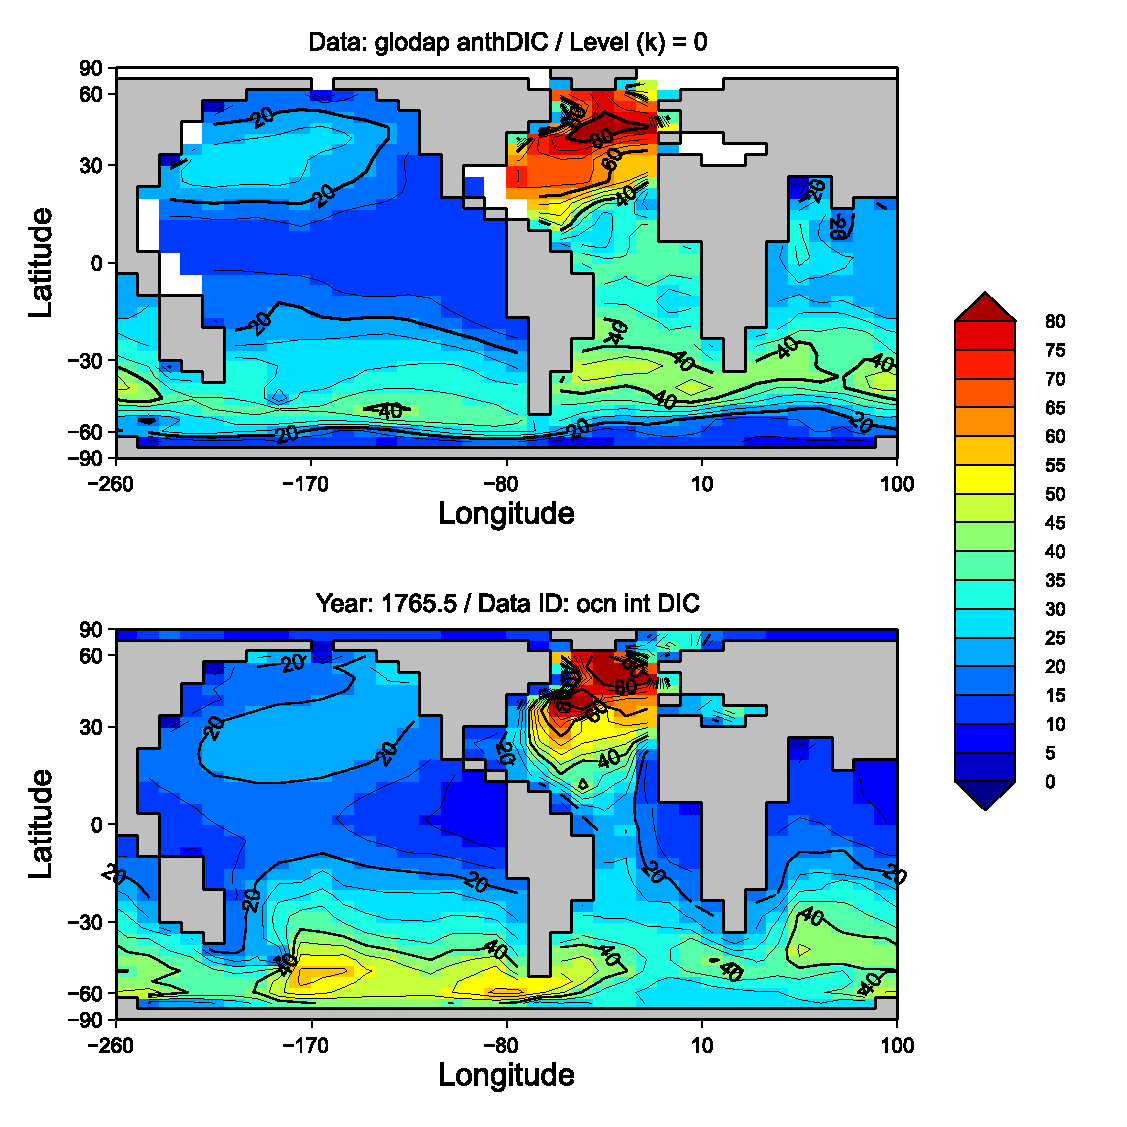
\includegraphics[scale=0.55]{chx-co2uptake.eps}
\end{center}
\vspace{-10pt}
\caption{Observed (top) \textit{vs.} Model (bottom) anthropogenic \(CO_{2}\) inventories.
Data and model water column integrals in units of mol \(CO_{2}\) m$^{-2}$ and are nominally with respect to year 1994.}
\label{fig:chx-co2uptake}
\end{figure}

\vspace{1mm}
\noindent\rule{4cm}{0.1mm}
\vspace{2mm}

\noindent Finally, and the closest to being slightly interesting: rather than applying highly idealized pulses  of \(CO_{2}\) emissions, the IPCC 'SRES' emissions scenarios can be used to make future projections with. An example forcing of this sort is provided and can be selected by changing the name of the forcing selection parameter (\texttt{bg\_par\_forcing\_name}) to:
\vspace{-2pt}\begin{verbatim}
worjh2.FeMahowald2006.FpCO2_Fp13CO2_A2_02180PgC
\end{verbatim}\vspace{-2pt}
which gives you the IPCC ‘A2’ scenario (extended beyond year 2010 in this case to give a total cumulative fossil fuel burn of 2018 PgC, e.g. \textit{Ridgwell and Schmidt} [2010]).
Again, as this forcing has units of \(PgCyr^{-1}\) in its time-series file, you will need to add a scaling parameter to the \textit{user-config} file to turn units of \(PgCyr^{-1}\) into \(mol C yr^{-1}\), i.e.,
\vspace{-2pt}\begin{verbatim}
bg_par_atm_force_scale_val_3=8.3333e+013
\end{verbatim}\vspace{-2pt}

For complete ‘realism’, you will need to run this experiment starting from the end of the historical transient experiment you have just run (Section 1.6), e.g.,
\vspace{-2pt}\begin{verbatim}
$ ./runmuffin.sh cgenie.eb_go_gs_ac_bg.worjh2.BASE LABS
   LAB_3.future 90 LAB_3.historical
\end{verbatim}\vspace{-2pt}
and with the start from year now set to year 2010 (the end year of the historical transient):
\vspace{-2pt}\begin{verbatim}
bg_par_misc_t_start=2010.0
\end{verbatim}\vspace{-2pt}
Note that the \textit{user-config} \footnotesize\textsf{LAB\_3.future }\normalsize is not provided for you – you will need to create this (or a file named whatever you like) by copying e.g., \footnotesize\textsf{LAB\_3.EXAMPLE }\normalsize and making the parameter changes described above (forcing specification parameter, emissions scaling parameter, and start year parameter).

You can also easily replace the details of the emissions with other SRES scenarios – simply find the year \textit{vs.} emissions rate information from the interweb\footnote{e.g., http://sres.ciesin.columbia.edu/final\_data.html} and edit or copy-and-paste the flux values for each decade into the file \footnotesize\textsf{biogem\_force\_flux\_atm\_pCO2\_sig.dat }\normalsize in the forcing directory.\textbf{ muffin} will then automatically interpolate between the decadal tie-points to give a continuous change in emissions. Now you are able to make a rather more realistic/plausible assessment of when and where potential ecological impacts (via assumed ocean chemistry criteria) might occur.

Try running (e.g. as jobs submitted to the cluster queue), some other actual or made up SRES emissions scenarios.

%------------------------------------------------

\newpage

%------------------------------------------------

\section{Further ideas}

%------------------------------------------------

\subsection{Assessing the importance of emissions rate}

By editing the flux and/or timing information you can control the \(CO_{2}\) emissions trajectory and total fossil fuel burned. Explore different \(CO_{2}\) release assumptions and note their impact on climate and ocean biogeochemistry. Much more realistic and appropriate to our \textit{current} global experiment is a lower rate (order of 10 or 20 \(PgCyr^{-1}\)) released over a longer interval (order of 100 years) compared to the conceptual 1000 \(PgC\) near-instantaneous pulse. Because the experiments are getting longer to run in real time … remember to make appropriate use of the cluster queuing facility – i.e., think about whether you want to sit around starting at the screen for 15 minutes waiting for a new line of numbers appear – if not: submit to the cluster queue. For instance, one might try and address the question: “For a given total release of  fossil fuel \(CO_{2}\), is it safer to burn it slower?” The answer is maybe not completely obvious, as burning carbon resources slower will result in a small global impact, but perhaps one that persists for longer. You could conceive of an ensemble (set) of model experiments, maybe one of 100 \(PgCyr^{-1}\) for 1 yr, one of 10 \(PgCyr^{-1}\) for 10 years, and one of 1 \(PgCyr^{-1}\) for 100 years, and run them all for e.g., 100 years.\footnote{These all represent rather unrealistically small total \(CO_{2}\) releases and you may want ot consider a total more like 1000 \(PgC\) or rather more. You may also want to think about more realistic shapes rather than pulses, such a some sort of ramp up and then down in the emissions rate (but for the same total emissions).} (As jobs submitted to the queue, all can be run simultaneously (with blank spaces between commands!).) (Don’t forget the control experiment!) 

Note note that you should create 3 new \textit{forcings} based on the original if you are editing the same original  \textit{forcing} and expecting to run different ones at the same time. Really, this is little more than copying and renaming \textit{user-config} files, except it involves entire directories in genie-forcings. Remember that the forcing is specified by the directory name assigned to \texttt{bg\_par\_forcing\_name} (enclosed in \texttt{''}).

%------------------------------------------------

\subsection{Determining thresholds of environmental impact}

There are various concerns about the impacts of continuing fossil fuel \(CO_{2}\) emissions and a number of proposed climatic (e.g., the 2 degree C global warming limit often mentioned in policy documents) and ecological ‘tipping points’. You can assess the maximum allowable \(CO_{2}\) emissions to remain within particular global environmental limits in the model. For example:

\begin{itemize}[noitemsep]

\vspace{1mm}
\item What is the maximum total \(CO_{2}\) release that can be made without inducing aragonite under-saturation at the ocean surface anywhere (or any season – see Section 5.2.3 in the User Manual for seasonal time-slice data saving)? How important is the time-scale of emissions in determining this? For total emissions above this: where in the ocean does the surface first become under-saturated? How large would the emissions have to be in order to induce under-saturation at the surface in the tropics (home to socio-economically important reef systems). These are questions that can be addressed with simple \(CO_{2}\) release experiments in ocean carbon cycle models and everyone seems to get a GRL paper out of it each and every time!

\vspace{1mm}
\item How important are \(CO_{2}\)-climate feedbacks in amplifying or diminishing future climate and ocean carbonate chemistry changes – e.g., is the same atmospheric p\(CO_{2}\) value reached with and without climate feedback (and surface warming) – if not, why? You can investigate this by contrasting an experiment made including \(CO_{2}\)-climate feedback with one made without. The \(CO_{2}\)-climate feedback can be turned off by setting: \texttt{ea\_36=n}.

\vspace{1mm}
\item Also: How much \(CO_{2}\) emission does it take to significantly ‘collapse’ the AMOC and over what time-scale? (Or alternatively: what is the atmospheric p\(CO_{2}\) threshold for collapse?) 
\\ If the AMOC weakens or collapses … why in the absence of a prescribed freshwater perturbation does this happen? What physical process are at play in response to rapid \(CO_{2}\) release too the atmosphere that may act to reduce or shutdown deep-water formation in the ocean model? (Plotting appropriate ocean property anomalies between the \(CO_{2}\) release experiment and a control experiment might help.)

\end{itemize}

\vspace{1mm}
Experiments could be hypothetical and consisting of \(CO_{2}\) pulses or ramps (or exponentials) and run on directly from a pre-industrial spin-up, or more ‘realistic’ and run on from the end of a historical transient experiment (e.g., starting in year 2010).

%----------------------------------------------------------------------------------------
%       CHAPTER X
%----------------------------------------------------------------------------------------

\cleardoublepage

\chapterimage{chx-biogeo.png} % Chapter heading image

\chapter{Ocean biogeochemical cycles}

\hfill \break

\vspace{24mm}

\noindent 

%------------------------------------------------

\newpage

%------------------------------------------------

\section*{READ.ME}


%------------------------------------------------

\newpage

%------------------------------------------------

\section{xxx}


%------------------------------------------------

\newpage

%------------------------------------------------

\section{xxx}


%------------------------------------------------

\subsection{Further modifications of the biological pump in the ocean}

Other manipulations of the biological pump and ocean carbon cycle are possible and potentially instructive and in the following examples may be of rather more relevance to past climates and carbon cycles and e.g. possible reasons for the low atmospheric \(CO_{2}\) concentrations at the last glacial, as opposed to relevant to geoengineering (a good thing!). The first two of these may have profound effects not only atmospheric p\(CO_{2}\) but also on dissolved oxygen concentrations in the ocean (and hence implications for the suitability of animal habitat such as for fish) and this is something that you will want to look at as part of your overall assessment of impacts.

\subsubsection*{Remineralization depth}

In the model configuration that you have been using, the degradation of particulate organic matter sinking in the water column proceeds according to a fixed profile of flux with depth (there is no e.g. temperature control on the rate of bacterial degradation of sinking organic matter) with \(CO_{2}\) and \(PO_{4}\) released back to the seawater as the particulate flux decreases. The parameter that controls the (\textit{e}-folding) depth scale of particulate organic matter is:
\vspace{-2pt}\small\begin{verbatim}
bg_par_bio_remin_POC_eL1=589.9451
\end{verbatim}\normalsize\vspace{-2pt}
Either edit this value (found under the heading: \texttt{\# --- REMINERALIZATION ---}) or add a new line at the end of the \textit{user-config} file specifying the value you want. Units are \(m\).

Read \textit{Ridgwell et al.} [2007] for additional discussion of this parameter. See Figure 2-4 in \textit{Ridgwell} [2001] (http://www.seao2.org/pubs/ridgwell\_thesis.pdf) for an illustration of how the flux of particulate organic matter decreases with depth in the ocean, plus references therein.

There is also an associated parameter: \texttt{bg\_par\_bio\_remin\_POC\_frac2}, which sets a fraction of organic matter that is assumed to settle through the water column completely un-altered (currently assigned a value of 0.045 == 4.5\%), but this is arguably less useful to change than the remineralization length-scale of the more labile fraction (the other 95.5\% of particulate organic carbon exported from the ocean surface).

Note that there may well be no simple parallel that can be found in geoengineering to this process. However, there are hypotheses that during the last glacial and as a result of colder ocean temperatures, the depth scale was longer. Conversely, there are ideas about that the warmer temperatures of the e.g. Eocene ocean and hence faster rates of bacterial metabolism led to a much shallower remineralization depth scale. So a remineralization depth scale that is responsive to temperature may have importance in understanding ocean biogeochemical cycles during both past warm and cold climates as well as obviously, future global change. While you are not implementing a temperature-dependent parameterization explicitly, you can at least test for whether changes in temperature might have important impacts by simply changing the remineralization depth to be shallower (smaller depth-scale under a warming climate) or deeper (greater depth-scale in a colder ocean).

\subsubsection*{Macro nutrient inventory and uptake}

Suggestions have been made that nutrients were used more efficiently during the LGM, meaning that for the same nutrient uptake at the surface more carbon was exported to depth in the ocean. See: \textit{Omta et al.} [2006]. There are also a bunch of (relatively old) hypotheses concerning differences between glacial and modern ocean in how much nitrate (\(NO^{-}_{3}\)) there was. There is no \(NO^{-}_{3}\) in this version of \textbf{muffin} (just \(PO_{4}\) and \(Fe\)), but an analogous change can be made to the phosphorous cycle.

For the nutrient-to-carbon ratio in organic matter, the relevant parameter is:
\vspace{-2pt}\small\begin{verbatim}
bg_par_bio_red_POP_POC=106.0
\end{verbatim}\normalsize\vspace{-2pt}
To change the default value (106.0), add a new line at the end of the \textit{user-config} file specifying the value you want. A larger number means that \(PO_{4}\) is being utilized more efficiently and more organic matter is being produced for the same nutrient consumption.

To test the effect of there being more \(PO_{4}\) in the ocean, in addition to using the (surface) flux forcing as described earlier, it is also possible to simply increase the inventory of the ocean as a whole in one go:
\vspace{-2pt}\small\begin{verbatim}
bg_ocn_dinit_8=1.0E-6
\end{verbatim}\normalsize\vspace{-2pt}
which will add \(1\:\mu mol\:kg^{-1}\) of \(PO_{4}\) uniformly to the ocean. (A larger/smaller number will obviously increase the glacial nutrient inventory by more/less.)

In terms of geoengineering, changing the ‘Redfield’ ocean plankton might be difficult … but not impossible, although we are presumably talking about releases of genetically modified organisms to the entire ocean to achieve this meaning there are obviously some severe ethical concerns. However, adding macro nutrients such as \(PO_{4}\) (more often, \(NO^{-}_{3}\) is talked about) may be more feasible.

\subsubsection*{CaCO3:POC rain ratio}

Kicked off by a classic 1994 \textit{Nature} paper by \textit{Archer and Maier-Reimer} (see: \textit{Kohfeld and Ridgwell} [2009]), one potential means of changing atmospheric \(CO_{2}\) naturally at the last glacial involves changes in the export ratio between \(CaCO_{3}\) (shells) and \(POC\) (particulate organic matter). Such a change in ratio could come about through a variety of ways (e.g., via the 'silica leakage hypothesis' (see: \textit{Kohfeld and Ridgwell} [2009]) and also through the direct effect of \(Fe\) on diatom physiology (see \textit{Watson et al.} [2000] in \textit{Nature} and also Supplemental Information). There are also ideas about an opposite ocean acidification effect, whereby the less acidic glacial (compared to modern) ocean led to increased calcification and \(CaCO_{3}\) export. Note that this response (higher saturation == greater rate of calcification) is encoded into your model configuration – see \textit{Ridgwell et al.} [2007b].

In \textbf{muffin}, the \(CaCO_{3}:POC\) rain ratio is controlled (technically: scaled) by the parameter:
\vspace{-2pt}\small\begin{verbatim}
bg_par_bio_red_POC_CaCO3=0.0485
\end{verbatim}\normalsize\vspace{-2pt}

The pattern of \(CaCO_{3}:POC\) rain ratio is not uniform across the ocean (why? (see: \textit{Ridgwell et al.} [2007, 2009]), and its pattern can be viewed in the (2D \textbf{BIOGEM}) netCDF variable: \textsf{\footnotesize misc\_sur\_rCaCO3toPOC}.

(Note that it is unlikely that there is any parallel in a geoengineering context to this process.)

%----------------------------------------------------------------------------------------
%       CHAPTER X
%----------------------------------------------------------------------------------------

\cleardoublepage

\chapterimage{geoengineering.png} % Chapter heading image

\chapter{Geoengineering I}

\hfill \break

\vspace{12mm}

\noindent In this Chapter we'll use the 'excuse' of geoengineering, to perturb and elucidate the response of the global carbon cycle and climate system and hence learn something new/different about Earth system dynamics compared to e.g. its response only under standard future carbon emissions scenarios.

%------------------------------------------------

\newpage

%------------------------------------------------

\section*{READ.ME}

You will need to download a new \textit{restart} file prior to embarking on the experiments. This differs from previous provided restarts in that it now includes an iron cycle in the ocean and hence co-limitation of biological productivity by Fe.
\vspace{-2mm}
\begin{verbatim}
$ wget http://www.seao2.info/cgenie_output/LAB_4.SPIN.tar.gz
\end{verbatim}

Extract the results in the usual way and in the usual place ... and return to \texttt{genie-main}.

%------------------------------------------------

\newpage

%------------------------------------------------

\section{Ocean carbon geoengineering}

In the following experiments you are going to explore some of the ocean biological controls on atmospheric p\(CO_{2}\) (plus ocean acidification, and the distributions and intensities of oxygen minimum zones). Really, the ‘geoengineering’ focus is just an excuse to be looking at how the biological pump in the ocean works, how it regulates atmospheric p\(CO_{2}\), how sensitive it is to perturbation and what the consequences are of any changes in it. So if you are uncomfortable with ideas of large scale manipulating the Earth system, you might instead think about the relevance of the experiments to e.g. understanding why atmospheric p\(CO_{2}\) was low at the time of the last glacial.

The overall idea of this Chapter is to run future \(CO_{2}\) emissions scenarios and test whether ocean carbon geoengineering is an effective means for reducing future ocean acidification and marine ecological impacts (but keeping in mind that you are also exploring the basic natural operation of the system in doing so). You will require a pre-industrial \textit{spin-up} and will need to create a new historical p\(CO_{2}\) transient experiment because you are now using a different \textit{base-config} (\texttt{cgenie.eb\_go\_gs\_ac\_bg.worjh2.BASEFe}) that includes additional tracers for the marine iron cycle, i.e. you cannot simply use any of the experiments from previous labs as a restart.

Refer to Section 12.6  for a guide as to what to ‘look for’ in the model results.

\vspace{1mm}
\noindent\rule{4cm}{0.1mm}
\vspace{2mm}

\noindent So to start with, go ahead and run a new historical transient experiment. A \textit{user-config} is provided for your convenience (\texttt{LAB\_4.historical}) … but maybe check the settings for e.g. start year, as well as note that there are a number of new parameters to control the iron cycle (amongst other differences) as compared to before: 
\vspace{-2pt}\begin{verbatim}
$ ./runmuffin.sh cgenie.eb_go_gs_ac_bg.worjh2.BASEFe LABS
   LAB_4.historical 245 LAB_4.SPIN
\end{verbatim}\vspace{-2pt}
(ignore the ‘WARNING’s at the start)

\vspace{1mm}
\noindent\rule{4cm}{0.1mm}
\vspace{2mm}

\noindent The provided example \textit{user-config} -- \texttt{LAB\_4.EXAMPLE} -- includes parameter settings for controlling any one of 3 different possible ocean carbon geoengineering schemes, described below. By default, these are commented out (== ignored by the model) and only the forcing for the A2 emissions scenario (\texttt{worjh2.FeMahowald2006.FpCO2\_Fp13CO2\_A2\_02180PgC}) with no geoengineering enacted,  is enabled by default. You might regard this as a control (reference) experiment for all the with-geoengineering experiments you might run, i.e. the impacts of \(CO_{2}\) emissions in the absence of any mitigation by geoenginerring. To activate any particular geoengineering forcing: simply un-comment (delete the \# at the start of) the appropriate pair of lines (the first line being the forcing specification, and the second one the total flux forcing used in the geoengineering scheme). If you have multiple (un-commented) settings of a parameter (e.g. \texttt{bg\_par\_forcing\_name}), then the value specified in the last occurrence of the parameter, is the one that is applied. This can get confusing, so if you un-comment out one set of parameter options, comment out (add a \# to) the ones you are not using.

The geoengineering (and control) experiments need to be run starting from the end of your historical transient experiment:
\vspace{-2pt}\begin{verbatim}
$ ./runmuffin.sh cgenie.eb_go_gs_ac_bg.worjh2.BASEFe LABS
   LAB_4.EXAMPLE 90 LAB_4.historical
\end{verbatim}\vspace{-2pt}
Because with a modern configuration and additional tracers in the ocean, the model is running rather slower than in some earlier exercises, you may not want to run beyond the end of the century (hence the 90 year experiment duration, starting from year 2010, as suggested above).

\vspace{1mm}
\noindent\rule{4cm}{0.1mm}
\vspace{2mm}

\noindent Each of the example geoengineering scenarios are delineated by its own specific forcing – a set of files that live in a uniquely named sub-directory within genie-forcings. The three forcings are:

\vspace{2mm}
\begin{itemize}[noitemsep]
\item 
\begin{verbatim}worjh2.FeMahowald2006.FpCO2_Fp13CO2_A2_02180PgC_FFe\end{verbatim}
\item 
\begin{verbatim}worjh2.FeMahowald2006.FpCO2_Fp13CO2_A2_02180PgC_FPO4\end{verbatim}
\item 
\begin{verbatim}worjh2.FeMahowald2006_FpCO2_Fp13CO2_A2_02180PgC_FALK\end{verbatim}
\end{itemize}
\vspace{2mm}
   
Each forcing includes the A2 \(CO_{2}\) emissions scenario, with the annual emissions (\(CO_{2}\) flux) \texttt{biogem\_force\_flux\_atm\_pCO2\_sig.dat} in units of \(PgCyr^{-1}\) (== GtC yr-1), hence requiring a units conversion setting in the \textit{user-config} (\texttt{bg\_par\_atm\_force\_scale\_val\_3=8.3333e+013}) that is provided for you under the heading \texttt{\# CO2 emissions scaling}. (You can completely ignore the carbon isotope settings.)

Each forcing also includes a prescribed dust flux to the ocean surface (the \texttt{FeMahowald2006} part of the directory name string). This is necessary because the model configuration you are using includes a co-limitation of biological productivity by iron (Fe) in addition to phosphate (\(PO_{4}\)). (The files associated with the dust forcing are: \texttt{biogem\_force\_flux\_sed\_det\_sig.dat} and \texttt{biogem\_force\_flux\_sed\_det\_SUR.dat} but you do not need to edit these files.) For the role of iron in controlling ocean productivity: possible starting points for background reading are: \textit{Ridgwell and Kohfeld} [2007] (PDF available form my website) or \textit{Jickells et al.} [2005] (Science).

\vspace{1mm}
The specific details of the 3 different example geoengineering scenarios are as follows:

%------------------------------------------------

\subsection{Iron fertilization}

\textit{Forcing}: \textsf{\footnotesize worjh2.FeMahowald2006.FpCO2\_Fp13CO2\_A2\_02180PgC\_FFe} \vspace{1pt}
\\-- a constant (with time) flux of dissolved Fe (in addition to whatever Fe dissolves into the surface ocean from the dust flux) is specified in: \texttt{biogem\_force\_flux\_ocn\_Fe\_sig.dat}. The magnitude of the applied flux is then scaled in the \textit{user-config} file by the setting:
\small\begin{verbatim}
bg_par_ocn_force_scale_val_9=1.0e+09
\end{verbatim}\normalsize
Note that this is simply an example total global flux. You might consider higher or lower fluxes, as well as potentially how ‘practical’ the annual production and supply of such quantities might be.

A spatial pattern of the flux is also defined, in the file:
\small\begin{verbatim}
biogem_force_flux_ocn_Fe_SUR.dat
\end{verbatim}\normalsize

An example pattern is set (see later for instructions on modifying this) with a row of grid cells  marked along the same latitude in the Southern Ocean. You do not need to retain this pattern. In choosing an alternative: think about where in the modern ocean biological productivity is thought to be at least partly limited by the availability of dissolved Fe. Remember that the model may or may not correspond with reality, i.e. it may or may not predict Fe limitation in the correct regions, which may affect your choice of location for iron fertilization.

%------------------------------------------------

\subsection{Phosphate fertilization}

\textit{Forcing}: \textsf{\footnotesize worjh2.FeMahowald2006.FpCO2\_Fp13CO2\_A2\_02180PgC\_FPO4} (‘macro-nutrient’ addition) 
\vspace{1pt}
\\ -- a constant (with time) flux of dissolved \(PO_{4}\) is specified in: \texttt{biogem\_force\_flux\_ocn\_PO4\_sig.dat}. The magnitude of the applied flux is then scaled in the \textit{user-config} by the setting:
\vspace{-2pt}\small\begin{verbatim}
bg_par_ocn_force_scale_val_8=2.0e+12 
\end{verbatim}\normalsize\vspace{-2pt}

Again, you should consider this as an example total flux. In choosing a total flux to apply, points of comparison include whatever the total weathering flux (via rivers) of P to the global ocean is. Also: global phosphate (fertilizer) production, which produces an interesting potential conflict between geoengineering and food production, although there are proposals for using fertilized ocean regions for enhanced fish production. 

A spatial pattern of the flux is also defined, in the file:
\vspace{-2pt}\small\begin{verbatim}
biogem_force_flux_ocn_PO4_SUR.dat
\end{verbatim}\normalsize\vspace{-2pt}

An example pattern has been set – here, the Equatorial Atlantic. In choosing your regions(s), think about where in the ocean (again – there may be differences between real ocean and model) productivity is currently limited by \(PO_{4}\). Also be aware of possible on-set of Fe limitation if you relieve the PO4 limitation (i.e., you could potentially lose effectiveness if you supply too much PO4 and instead productivity and \(CO_{2}\) draw-down is capped by a second factor). You could potentially consider PO4 and Fe addition at the same time … ?

%------------------------------------------------

\subsection{Enhanced weathering}

\textit{Forcing}: \textsf{\footnotesize worjh2.FeMahowald2006.FpCO2\_Fp13CO2\_A2\_02180PgC\_FPO4} (alkalinity addition)
\vspace{1pt}
\\ -- a constant (with time) flux of alkalinity is specified in: \texttt{biogem\_force\_flux\_ocn\_ALK\_sig.dat}. The magnitude of the applied flux is then scaled in the \textit{user-config} by the setting:
\vspace{-2pt}\small\begin{verbatim}
bg_par_ocn_force_scale_val_12=5.0e+13
\end{verbatim}\normalsize\vspace{-2pt}

Again, another example total flux. In choosing a total flux to apply, points of comparison include whatever the total weathering flux (via rivers) of alkalinity (often described in terms of the bicarbonate ion flux) to the global ocean is. Also: global cement (lime) production. (Note that in one mole of lime: \(CaO\), you have 2 moles of alkalinity (\(Ca^{2+}\)).) 

A spatial pattern of the flux is also defined, in the file:
\vspace{-2pt}\small\begin{verbatim}
biogem_force_flux_ocn_ALK_SUR.dat
\end{verbatim}\normalsize\vspace{-2pt}

An example pattern has been set – here, bordering the major tropical coral reefs locations in the Western Pacific. In choosing your regions(s), you might think about mitigating specific ecosystem impacts of ocean acidification, or about the feasibility of transport and proximity to abundant limestone (\(CaCO_{3}\) – the source of lime) and/or energy.

%------------------------------------------------

\subsection{Modifying spatial patterns}

The spatial patterns of an applied flux forcing to the ocean can easily be modified. The pattern is specified in a simple ASCII (plain text) file, in the file in the forcing sub-directory ending ‘\texttt{\_SUR.dat}’. The file (in this example the default Fe pattern) looks like:

\newpage

\tiny\begin{verbatim}
0.0 0.0 0.0 0.0 0.0 0.0 0.0 0.0 0.0 0.0 0.0 0.0 0.0 0.0 0.0 0.0 0.0 0.0 0.0 0.0   0   0   0   0 0.0 0.0 0.0 0.0 0.0 0.0 0.0 0.0 0.0 0.0 0.0 0.0
  0   0   0   0   0   0   0   0   0 0.0   0   0   0   0   0   0   0   0   0 0.0 0.0   0   0 0.0 0.0 0.0 0.0 0.0   0   0   0   0   0   0   0   0
  0   0   0   0   0   0 0.0 0.0 0.0 0.0 0.0 0.0   0   0   0   0   0   0   0   0 0.0 0.0 0.0 0.0 0.0 0.0   0   0   0   0   0   0   0   0   0   0
  0   0   0   0 0.0 0.0 0.0 0.0 0.0 0.0 0.0 0.0 0.0   0   0   0   0   0   0   0 0.0 0.0 0.0 0.0 0.0   0   0   0   0   0   0   0   0   0   0   0
  0   0   0   0 0.0 0.0 0.0 0.0 0.0 0.0 0.0 0.0 0.0 0.0   0   0   0   0   0   0 0.0 0.0 0.0 0.0 0.0 0.0   0   0   0   0   0   0   0   0   0   0
  0   0   0 0.0 0.0 0.0 0.0 0.0 0.0 0.0 0.0 0.0 0.0 0.0   0   0   0   0   0 0.0 0.0 0.0 0.0 0.0 0.0 0.0   0   0   0   0   0   0   0   0   0   0
  0   0   0 0.0 0.0 0.0 0.0 0.0 0.0 0.0 0.0 0.0 0.0 0.0   0   0   0   0 0.0 0.0 0.0 0.0 0.0 0.0 0.0   0 0.0 0.0   0   0   0   0   0   0   0   0
  0   0   0 0.0 0.0 0.0 0.0 0.0 0.0 0.0 0.0 0.0 0.0 0.0   0   0   0   0 0.0 0.0 0.0 0.0 0.0 0.0 0.0 0.0 0.0 0.0 0.0 0.0   0   0   0   0   0   0
  0   0 0.0 0.0 0.0 0.0 0.0 0.0 0.0 0.0 0.0 0.0 0.0 0.0 0.0   0   0   0 0.0 0.0 0.0 0.0 0.0 0.0 0.0   0   0 0.0 0.0   0   0   0   0   0   0   0
  0   0 0.0 0.0 0.0 0.0 0.0 0.0 0.0 0.0 0.0 0.0 0.0 0.0 0.0   0 0.0 0.0 0.0 0.0 0.0 0.0 0.0 0.0 0.0   0   0   0   0   0   0   0   0   0   0   0
  0   0 0.0 0.0 0.0 0.0 0.0 0.0 0.0 0.0 0.0 0.0 0.0 0.0 0.0   0 0.0 0.0 0.0 0.0 0.0 0.0 0.0 0.0 0.0   0   0   0   0   0   0 0.0 0.0   0   0   0
  0 0.0 0.0 0.0 0.0 0.0 0.0 0.0 0.0 0.0 0.0 0.0 0.0 0.0 0.0   0 0.0 0.0 0.0 0.0 0.0 0.0 0.0 0.0 0.0   0   0   0   0   0   0 0.0 0.0   0   0   0
  0 0.0 0.0 0.0 0.0 0.0 0.0 0.0 0.0 0.0 0.0 0.0 0.0 0.0 0.0 0.0   0 0.0 0.0 0.0 0.0 0.0 0.0 0.0 0.0   0   0   0   0   0   0 0.0 0.0   0 0.0 0.0
  0 0.0 0.0 0.0 0.0 0.0 0.0 0.0 0.0 0.0 0.0 0.0 0.0 0.0 0.0 0.0 0.0   0 0.0 0.0 0.0 0.0 0.0 0.0 0.0   0   0   0   0   0   0 0.0 0.0 0.0 0.0 0.0
  0 0.0 0.0 0.0 0.0 0.0 0.0 0.0 0.0 0.0 0.0 0.0 0.0 0.0 0.0 0.0 0.0 0.0   0 0.0 0.0 0.0 0.0 0.0 0.0   0   0   0   0   0   0 0.0 0.0 0.0 0.0 0.0
  0 0.0 0.0 0.0 0.0 0.0 0.0 0.0 0.0 0.0 0.0 0.0 0.0 0.0 0.0 0.0 0.0 0.0   0   0 0.0 0.0 0.0 0.0 0.0   0   0   0   0   0   0 0.0 0.0 0.0 0.0 0.0
  0 0.0 0.0 0.0 0.0 0.0 0.0 0.0 0.0 0.0 0.0 0.0 0.0 0.0 0.0 0.0 0.0 0.0   0   0 0.0 0.0 0.0 0.0 0.0 0.0 0.0   0   0   0 0.0 0.0 0.0 0.0 0.0 0.0
  0   0 0.0 0.0 0.0 0.0 0.0 0.0 0.0 0.0 0.0 0.0 0.0 0.0 0.0 0.0 0.0 0.0   0   0   0 0.0 0.0 0.0 0.0 0.0 0.0   0   0   0 0.0 0.0 0.0 0.0 0.0 0.0
  0   0 0.0 0.0 0.0 0.0 0.0 0.0 0.0 0.0 0.0 0.0 0.0 0.0 0.0 0.0 0.0 0.0   0   0   0 0.0 0.0 0.0 0.0 0.0 0.0   0   0   0 0.0 0.0 0.0 0.0 0.0 0.0
0.0   0 0.0 0.0 0.0 0.0 0.0 0.0 0.0 0.0 0.0 0.0 0.0 0.0 0.0 0.0 0.0 0.0   0   0   0   0 0.0 0.0 0.0 0.0 0.0   0   0   0 0.0 0.0 0.0 0.0 0.0 0.0
0.0   0 0.0 0.0 0.0 0.0 0.0 0.0 0.0 0.0 0.0 0.0 0.0 0.0 0.0 0.0 0.0 0.0   0   0   0   0 0.0 0.0 0.0 0.0 0.0   0   0   0 0.0 0.0 0.0 0.0 0.0 0.0
0.0 0.0   0   0 0.0 0.0 0.0 0.0 0.0 0.0 0.0 0.0 0.0 0.0 0.0 0.0 0.0 0.0   0   0   0   0 0.0 0.0 0.0 0.0 0.0   0   0   0 0.0 0.0 0.0 0.0 0.0 0.0
0.0 0.0   0   0 0.0 0.0 0.0 0.0 0.0 0.0 0.0 0.0 0.0 0.0 0.0 0.0 0.0 0.0   0   0   0   0 0.0 0.0 0.0 0.0 0.0   0   0   0 0.0 0.0 0.0 0.0 0.0 0.0
0.0 0.0   0   0 0.0 0.0 0.0 0.0 0.0 0.0 0.0 0.0 0.0 0.0 0.0 0.0 0.0 0.0 0.0   0   0   0 0.0 0.0 0.0 0.0 0.0   0   0   0 0.0 0.0 0.0 0.0 0.0 0.0
0.0 0.0   0   0   0 0.0 0.0 0.0 0.0 0.0 0.0 0.0 0.0 0.0 0.0 0.0 0.0 0.0 0.0   0   0   0 0.0 0.0 0.0 0.0 0.0   0   0 0.0 0.0 0.0 0.0 0.0 0.0 0.0
0.0 0.0   0   0   0 0.0 0.0 0.0 0.0 0.0 0.0 0.0 0.0 0.0 0.0 0.0 0.0 0.0 0.0   0   0 0.0 0.0 0.0 0.0 0.0 0.0 0.0   0 0.0 0.0 0.0 0.0 0.0 0.0 0.0
0.0 0.0   0   0   0 0.0 0.0 0.0 0.0 0.0 0.0 0.0 0.0 0.0 0.0 0.0 0.0 0.0 0.0   0   0 0.0 0.0 0.0 0.0 0.0 0.0 0.0   0 0.0 0.0 0.0 0.0 0.0 0.0 0.0
0.0 0.0 0.0   0   0 0.0 0.0 0.0 0.0 0.0 0.0 0.0 0.0 0.0 0.0 0.0 0.0 0.0 0.0   0   0 0.0 0.0 0.0 0.0 0.0 0.0 0.0   0 0.0 0.0 0.0 0.0 0.0 0.0 0.0
0.0 0.0 0.0 0.0   0 0.0 0.0 0.0 0.0 0.0 0.0 0.0 0.0 0.0 0.0 0.0 0.0 0.0 0.0   0 0.0 0.0 0.0 0.0 0.0 0.0 0.0 0.0 0.0 0.0 0.0 0.0 0.0 0.0 0.0 0.0
0.0 0.0 0.0 0.0 0.0 0.0 0.0 0.0 0.0 0.0 0.0 0.0 0.0 0.0 0.0 0.0 0.0 0.0 0.0   0 0.0 0.0 0.0 0.0 0.0 0.0 0.0 0.0 0.0 0.0 0.0 0.0 0.0 0.0 0.0 0.0
0.0 0.0 0.0 0.0 0.0 0.0 0.0 0.0 0.0 0.0 0.0 0.0 0.0 0.0 0.0 0.0 0.0 0.0 0.0   0 0.0 0.0 0.0 0.0 0.0 0.0 0.0 0.0 0.0 0.0 0.0 0.0 0.0 0.0 0.0 0.0
0.0 0.0 0.0 0.0 0.0 0.0 0.0 0.0 0.0 0.0 0.0 0.0 0.0 0.0 0.0 0.0 0.0 0.0 0.0   0 0.0 0.0 0.0 0.0 0.0 0.0 0.0 0.0 0.0 0.0 0.0 0.0 0.0 0.0 0.0 0.0
0.0 0.0 0.0 0.0 0.0 0.0 0.0 0.0 0.0 0.0 0.0 0.0 0.0 0.0 0.0 0.0 0.0 0.0 0.0 0.0 0.0 0.0 0.0 0.0 0.0 0.0 0.0 0.0 0.0 0.0 0.0 0.0 0.0 0.0 0.0 0.0
1.0 1.0 1.0 1.0 1.0 1.0 1.0 1.0 1.0 1.0 1.0 1.0 1.0 1.0 1.0 1.0 1.0 1.0 1.0 1.0 1.0 1.0 1.0 1.0 1.0 1.0 1.0 1.0 1.0 1.0 1.0 1.0 1.0 1.0 1.0 1.0
  0 0.0 0.0 0.0 0.0 0.0 0.0 0.0 0.0 0.0 0.0 0.0 0.0 0.0 0.0 0.0 0.0 0.0 0.0 0.0 0.0 0.0 0.0 0.0 0.0 0.0 0.0 0.0 0.0 0.0 0.0 0.0 0.0 0.0 0.0   0
  0   0   0   0   0   0   0   0   0   0   0   0   0   0   0   0   0   0   0   0   0   0   0   0   0   0   0   0   0   0   0   0   0   0   0   0
\end{verbatim}\normalsize

Here: ‘\texttt{0}’s represent land and cannot have a forcing associated with them. ‘\texttt{0.0}’s represent a zero flux to the ocean, and ‘\texttt{1.0}’s the default Southern Ocean forcing pattern. Note that a distinction is made between a ‘\texttt{0}’ and a ‘\texttt{0.0}’ so that you can make out where the continents are and do not necessarily have to count in the \textit{i} and \textit{j} grid directions to find a specific location. The grid is the same as you saw previously in tracing ocean circulation, and which numbered the \textit{i} and \textit{j} axes if that helps. For the ALK forcing, ‘\texttt{1.0}’s are set off of the coast of Australia and SE Asia and in the \(PO_{4}\) forcing, in the Atlantic.

There is no more to changing the pattern of the flux forcing than simply marking with a ‘\texttt{1.0}’ where you would like the forcing applied, and a ‘\texttt{0.0}’ where it should not be. Note that there should be a single blank line at the bottom of the file. (If you have problems applying a modified spatial pattern – check that this is present.) It is best to keep a copy of the original forcing in case you make a mess of the spatial pattern file, but the original can also be recovered from the code server.

%------------------------------------------------

\newpage

%------------------------------------------------

\section{Further ideas}

%------------------------------------------------

\subsection{Impacts to look out for}

\begin{itemize}

\vspace{1pt}
\item Impacts and ecosystems of interest could potentially be ones residing on the ocean floor, such as cold-water (deep water) corals, and are not necessarily planktic (/surface) only.

\vspace{1pt}
\item Don’t forget that different calcifying organisms employ different mineralogies (calcite vs. aragonite), with different saturation states and hence potentially susceptibility to ocean acidification. Hence thresholds of both aragonite and calcite saturation will be relevant, depending on the organism. Depending on the organism, saturation changes occurring in specific regions may much more relevant than a global mean change. Also, it might be the seasonal minimum value reached, rather than annual averaged minimum, that is critical.

\vspace{1pt}
\item Some of the arguments against some forms of ocean carbon geoengineering concern the potential for adverse impacts on marine organisms (and positive climate feedbacks) induced by decreases in the degree of oxygenation in the ocean, such as expanding and/or intensifying oxygen minimum zones. \textbf{muffin} saves 3D fields of \(O_{2}\) concentrations that can be plotted in slices through the ocean of various orientations.

\end{itemize}

%------------------------------------------------

\subsection{Other thoughts and suggestions}

\begin{itemize}

\vspace{1pt}
\item If you want to combine forcings, you need to first update the file: \textsf{\footnotesize configure\_forcings\_ocn.dat} – this specifies which ocean flux forcing will be used – simply copy the relevant line from the equivalent file of the forcing to be added. You will also need to copy in the relevant ‘\texttt{\_sig.dat}’ and ‘\texttt{\_SUR.dat}’ files. Remember that in the \textit{user-config} file, you will need to set the relevant flux scaling parameter for each different flux in the forcing.

\vspace{1pt}
\item By default, the \(CO_{2}\)-climate feedback is ‘on’:
\vspace{-2pt}\small\begin{verbatim}
# set climate feedback
ea_36=y
\end{verbatim}\normalsize\vspace{-2pt}
Should you want to assess the impacts of geoengineering independently of changes in climate -- the option is there. (Note that under some of the high end \(CO_{2}\) emissions scenarios, there may be a degree of collapse of the AMOC that will presumably affect the patterns of ocean acidification and oxygenation etc.)

\vspace{1pt}
\item If you are having doubts that your experiment is actually ‘doing’ anything (different from the control) – remember to create anomaly maps (plots) to look for specific changes in e.g. saturation state, pH, or the water column inventory of anthropogenic \(CO_{2}\). Even before this – plot anomalies of the flux you think you have applied, looking specifically at the region you think you have applied it to. For this, \textbf{muffin} saves the 3D distributions of dissolved Fe and \(PO_{4}\). See Figures below.

\vspace{1pt}
\item Always be aware of the caveats regarding this specific model (and models in general) – how much does it different form the ‘real world’ for the modern ocean, particularly in terms of patterns of carbonate saturation? Does it even simulate anthropogenic \(CO_{2}\) uptake adequately in the first place?

\end{itemize}

\begin{figure}[ht]
\begin{center}
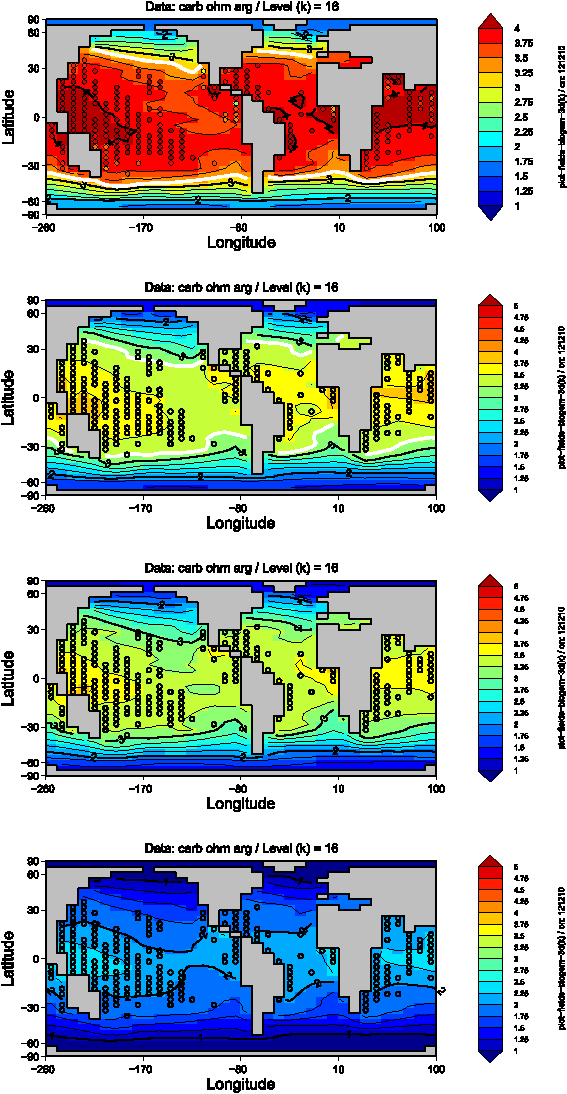
\includegraphics[scale=0.875]{chx-oaimpacts.eps}
\end{center}
\caption{
\textbf{Mean annual ocean surface saturation (aragonite) changes.}
Top: pre-industrial model ocean surface saturation (aragonite) with ReefBase tropical coral reef locations re-gridded to the \textbf{muffin} grid and color-coded with modern observationally-based saturation values.
2nd and 3rd down: Year 1994 and 2010 ocean surface saturation (aragonite) with ReefBase reef locations.
Bottom: Year 2010 ocean surface saturation (aragonite) under the A2 \(CO_{2}\) emissions scenario.
The thick white line delineates the 3.25 saturation contour (inferred to reflect a limitation on corals).
\textit{Examples here produced using \textbf{muffinplot} but equally do-able in \textbf{Panoply} with the exception of achieving a data overlay. These are provided simply to illustrate some of the impacts you might consider and possible ways of visualizing them.}
}
\label{fig:chx-oaimpacts}
\end{figure}

\begin{figure}[ht]
\begin{center}
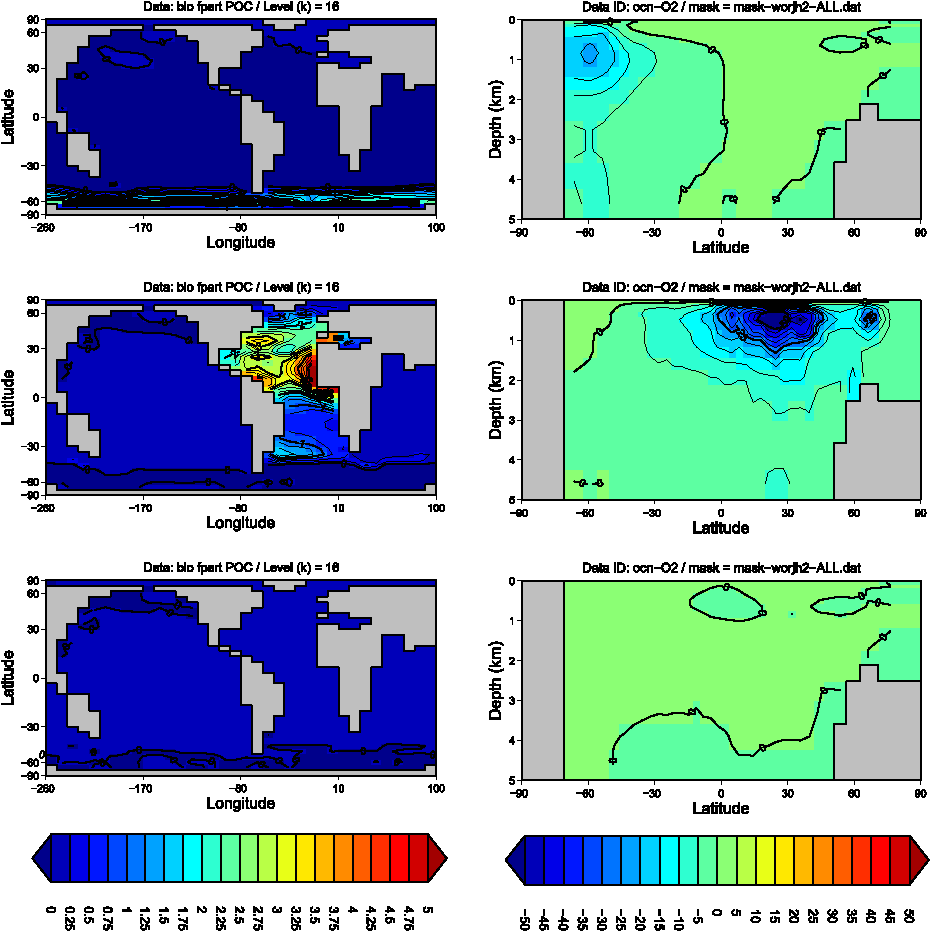
\includegraphics[scale=0.875]{chx-geoengimpacts.eps}
\end{center}
\caption{
\textbf{Ocean surface export (particulate organic carbon) and zonal \([O_{2}]\) anomalies.}
Left: anomalies of global mean annual export production, for \(Fe\) fertilization (top), \(PO_{4}\) addition (middle), and ocean liming (bottom).
Right: Zonal mean anomalies of dissolved \(O_{2}\) concentrations.
\textit{Examples here produced using \textbf{muffinplot} but equally do-able in \textbf{Panoply} with the exception of achieving a data overlay. These are provided simply to illustrate some of the impacts you might consider and possible ways of visualizing them.}
}
\label{fig:chx-geoengimpacts}
\end{figure}

%----------------------------------------------------------------------------------------
%       CHAPTER X
%----------------------------------------------------------------------------------------

\cleardoublepage

%\chapterimage{} % Chapter heading image

\chapter{Proxies and Reconstructing the Past}

\hfill \break

\vspace{24mm}

\noindent 

%------------------------------------------------

\newpage

%------------------------------------------------

\section*{READ.ME}


%------------------------------------------------

\newpage

%------------------------------------------------

\section{xxx}


%----------------------------------------------------------------------------------------
%       CHAPTER X
%----------------------------------------------------------------------------------------

\cleardoublepage

\chapterimage{spore-920.png} % Chapter heading image

\chapter{Marine ecosystems and dynamics}

\hfill \break

\noindent \textit{The following is based on workshop material originally devised by Ben Ward <b.a.ward@soton.ac.uk>}

\section*{Stuff to keep in mind\dots}
\begin{itemize}
\item We will be working with highly idealised ecosystems in a highly idealised ocean.
\item The aim is to explore why the model behaves as it does.
\item The assumption is that this will give us some insight into why the real world behaves as it does. Perhaps. (It is up to you to question the validity of this assumption.)
\end{itemize}

\section*{Background reading}
\begin{itemize}
\item \href{https://doi.org/10.5194/gmd-2017-258}{\textit{Ward et al.} [2017]} -- Ward, B. A., Wilson, J. D., Death, R. M., Monteiro, F. M., Yool, A., and Ridgwell, A.: EcoGEnIE 0.1: Plankton Ecology in the cGENIE Earth system model, \textit{Geosci. Model Dev. Discuss.}, https://doi.org/10.5194/gmd-2017-258, 2017.
\end{itemize}

%------------------------------------------------

\newpage

%------------------------------------------------

\section*{Read.me}

Before you start, you need to retrieve some model experiment \textit{restart} files. At the terminal, enter the  following commands (hitting `return' after each command):

\vspace{-2mm}
\footnotesize\begin{verbatim}
cd ~/cgenie_output
wget http://www.seao2.info/cgenie_output/_restarttest.worlg4.Wardetal20018.ECOGEM.SPIN.tar.gz
tar xfvz _restarttest.worlg4.Wardetal20018.ECOGEM.SPIN.tar.gz
\end{verbatim}\normalsize
\vspace{-2mm}

\noindent Then return to the \textbf{muffin} main directory:

\vspace{-2mm}
\small\begin{verbatim}
cd genie-main
\end{verbatim}\normalsize
\vspace{-2mm}

\noindent (\uline{Also before you start -- read the \textit{Ward et al.} reference.})

%------------------------------------------------

\newpage

%------------------------------------------------

\section{Getting going with ECOGEM}

Previously, you have run the standard 'biogeochemical' version of \textbf{muffin}, and biological export fluxes calculated via simple mass balance (and limitation) considerations by the module \textbf{BIOGEM}. In this chapter, we are going get started with the '\textbf{ECOGEM}' package. This will allow us to extend the capabilities of \textbf{muffin} to examine a range of questions relating to the role of physiology and community structure in regulating the biological pump. 

First, we need to understand the relationship and differences between \textbf{BIOGEM} and \textbf{ECOGEM}. 
In \textbf{BIOGEM}, the biological pump is driven by an implicit (i.e. unresolved) biological community. As in the real ecosystem, the biological uptake of carbon and nutrients (such as phosphorus and iron) is limited by light, temperature and nutrient availability. Unlike the real ecosystem, any uptake is \textit{directly} and \textit{instantly} returned to dissolved organic matter (DOM) and inorganic nutrients in the ocean interior.

\vspace{4mm}
\begin{itemize}
\item \underline{surface inorganic nutrients} $\xrightarrow[\rm and~export]{\rm production}$ \underline{DOM and deep inorganic nutrients}
\end{itemize}
\vspace{4mm}

In \textbf{ECOGEM}, biological uptake is again limited by light, temperature and nutrient availability, but here it must pass through an explicit and dynamic intermediary plankton biomass pool, before being returned to DOM or dissolved inorganic nutrients.

\vspace{4mm}
\begin{itemize}
\item \underline{surface inorganic nutrients} $\xrightarrow[]{\rm production}$ \underline{plankton biomass} $\xrightarrow[]{\rm export}$ \underline{DOM and deep inorganic nutrients}
\end{itemize}
\vspace{4mm}

%------------------------------------------------

\subsection{Running the model}

We will start with the simplest possible configuration of \textbf{ECOGEM}, with just a single phytoplankton class. You can run this model at the command line, by entering the following command (note that this should be one continuous line) \dots

\small\begin{verbatim}
$ ./runmuffin.sh muffin.CBE.worlg4.BASESFeTDTL LABS wardetal.2018.ECOGEM.EXAMPLE 10 
  _restarttest.worlg4.Wardetal20018.ECOGEM.SPIN
\end{verbatim}\normalsize

\noindent As before, we have five input parameters after  the run script (\texttt{./runmuffin.sh}) is invoked:

\vspace{2mm}
\begin{enumerate}[noitemsep]

\item \texttt{muffin.CBE.worlg4.BASESFeTDTL} $\rightarrow$ The `\textit{base-config}' file. \\
$~$\hfill Note the additional~`\texttt{\_eg}' that marks the inclusion of the \textbf{ECOGEM} package.

\item \texttt{LABS} $\rightarrow$ The \textit{user-config} directory where the \textit{user-config} file resides.

\item \texttt{wardetal.2018.ECOGEM.EXAMPLE} $\rightarrow$ The \textit{user-config} file (experiment name).

\item \texttt{10} $\rightarrow$ The run duration (for this particular example experiment), in years.

\item \texttt{\_restarttest.worlg4.Wardetal20018.ECOGEM.SPIN} $\rightarrow$ The \textit{restart} filename.
\\Here we are telling the model to start from the endpoint of a previous experiment (a 10,000 year run of \textbf{BIOGEM} ... although what you actually have, is a 10 year run following on from a 10,000 year run ...). Note that the \textit{restart} here only applies to the biogeochemical part of the model. The ecological community will be initialised from some very low biomass.

\end{enumerate}
\vspace{2mm}

The model will run as before, except that now we have the \textbf{ECOGEM} debug option enabled, and you will get a lot of extra information about how the ecological model is configured.
\vspace{1mm}

The extra lines, e.g.
\small\begin{verbatim}
>>> SAVING ECOGEM TIME-SLICE AVERAGE CENTERED @ year : 0.500
\end{verbatim}\normalsize
confirm that \textbf{ECOGEM} is writing ecological time-slices at the same time as \textbf{BIOGEM} is writing its own time slices. (\textbf{ECOGEM} is not currently set up to save time-series data in the same way as \textbf{BIOGEM}.)

%------------------------------------------------

\subsection{Viewing 2D time-slice output} 

Following the same convention as for \textbf{BIOGEM}, \textbf{ECOGEM} \textit{time-slice} output will be saved in the directory \texttt{\textasciitilde{}/cgenie\_output/wardetal.2018.ECOGEM.EXAMPLE/ECOGEM/}

\vspace{2mm}
\begin{enumerate}[noitemsep]

\item Open the \textsf{\small fields\_ecogem\_2D.nc} file by locating it in the correct directory, and double clicking on it in the file transfer window. Alternatively, you can open \textbf{Panoply} by selecting \textsf{\small File} $\rightarrow$ \textsf{\small Open}, and clicking through.

\item You should now see a list of 2D arrays that were output by \textbf{ECOGEM}. Looking at the \textsf{\small Long Name} description, simply click on a variable of interest. If a menu window pops up, just click on \textsf{\small Create} or hit the \textsf{\small Return} key.

\item Check the Panoply settings to make sure you really know what you are looking at.
\begin{enumerate}[noitemsep]
\item Which time-slice (i.e. simulation year) are you looking at?
\item What is the data range (i.e. colour scale)
\end{enumerate}

\item[NOTE:] You can change the default settings in \textbf{Panoply} to avoid changing things every time you open a new file. First click on \textsf{\small Panoply} $\rightarrow$ \textsf{\small Preferences...}. Here you can switch off interpolation and the grid overlay under the \textsf{\small General} menu. You can disable the spuriously precise coastline under \textsf{\small Lon-Lat Plots}.

\end{enumerate}
\vspace{2mm}

%------------------------------------------------

\subsection{Comparing to observations} 

Models are usually intended as an approximation of the real world (whatever that is). It might, therefore, be useful to check if our approximation is in anyway realistic. We can do this by comparing the model output to observations.

\vspace{2mm}
\begin{enumerate}[noitemsep]

\item You can download a compilation of key biogeochemical variables from the \textsf{\small mycenie} \href{http://www.seao2.info/cgenie/data/GEnIE_observations.nc}{webpage}.

\item You can open the \textsf{\small GEnIE\_observations.nc} file in \textbf{Panoply} in the same way as you opened the \textsf{\small fields\_ecogem\_2D.nc} file.

\item You can now compare the model output to key biogeochemical variables, such as surface chlorophyll or phosphate. (Also, e.g. create difference maps.)

\item Does the model perform well or poorly with respect to reproducing these variables?

\item[NOTE:] \textbf{ECOGEM} only saves a limited number of surface (2D) data arrays. You can look at other variables (in 2D and 3D) by opening the corresponding \textbf{BIOGEM} files, \textsf{\small fields\_biogem\_2D.nc} and \textsf{\small fields\_biogem\_3D.nc} in \textbf{Panoply}. They can be found in the directory:
\\ \texttt{\textasciitilde{}/cgenie\_output/wardetal.2018.ECOGEM.EXAMPLE/BIOGEM/}

\end{enumerate}
\vspace{2mm}

\noindent Bear in mind that we restarted the model from a previous simulation with \textbf{BIOGEM}. Some of the state variables may take a long time (i.e. $\gg$ 10 years) to adjust to the new model configuration (especially at depth). 
%------------------------------------------------

\newpage

%------------------------------------------------

\section{Ecosystem configuration}

In the last section you ran a very simple version of the ecosystem model, and compared it to observations. In this section we are going to add a bit more ecological realism, with the aim of improving model performance. We will start by adding a zooplankton population that  should bring a degree of `top-down' control to the phytoplankton population. 
\vspace{2mm}

Details of the original ecosystem are specified in the \textit{user-config} file:

\texttt{wardetal.2018.ECOGEM.EXAMPLE}.

\vspace{2mm}
\begin{enumerate}[noitemsep]

\item Locate the \textit{user-config} file (in \texttt{\textasciitilde{}/cgenie.muffin/genie-userconfigs/LABS}), and open it in your preferred text editor.

\item The \textit{user-config} file can be used to configure the model to your liking. One of the most important amendments to note straight away can be seen on line 11, \texttt{bg\_par\_bio\_prodopt="NONE"}. This effectively disables the biological pump in \textbf{BIOGEM}, replacing it with the explicit biology of \textbf{ECOGEM}. This is a necessary step whenever running \textbf{ECOGEM}, because we do not want the implicit and explicit biological schemes to be implemented in the same simulation.

\item We can also see a load of other model parameters. Any that begin with `\texttt{bg\_}' correspond to \textbf{BIOGEM}, while `\texttt{eg\_}' corresponds to \textbf{ECOGEM}. The \textbf{ECOGEM} parameters begin after line 71.

\item One of the most important parameters specifies the \textit{ecosystem configuration} file:
\small\begin{verbatim}
eg_par_ecogem_plankton_file ='NPD.eco'
\end{verbatim}\normalsize

This points to a file (located in \texttt{\textasciitilde{}/cgenie.muffin/genie-ecogem/data/input/}) that specifies every plankton population that is included at the start of the model run. If you open that file in the text editor, you will see something akin to the following:
\scriptsize\begin{verbatim}
 01                 02    03
 \/                 \/    \/

-START-OF-DATA-
 Phytoplankton    10.00   1
-END-OF-DATA-

 /\                 /\    /\
 01                 02    03

DATA FORMAT AND ORDER
---------------------

COLUMN #01: plankton functional type name
COLUMN #02: plankton diameter (micrometers)
COLUMN #03: number of randomised replicates

INFO: TRACER ASSIGNMENT RULES
-----------------------------
Plankton functional type one of: Prochlorococcus
                                 Synechococcus
                                 Picoeukaryote
                                 Diatom
                                 Coccolithophore
                                 Diazotroph
                                 Phytoplankton
                                 Zooplankton
                                 Mixotroph
\end{verbatim}\normalsize

\item The first thing to note is that only the lines in between the \texttt{\small -START-OF-DATA-} and \texttt{\small -END-OF-DATA-} tags are read by the computer. The rest is there solely for your guidance. 

Each line that is entered in the computer-readable area tells the model to put a distinct plankton population in the model. The ``plankton functional type'' of this population is specified in the first column, while the plankton diameter specified in the second column. A `\texttt{1}' must always be placed in the third column (it doesn't do anything, but the model still needs it).

In this `NPD' configuration, we only have a 10 micron generic phytoplankton. The ecological and physiological traits of this population are assigned automatically according to the size and the functional type. 

\item[NOTE:] The only PFTs available at the moment are \texttt{Phytoplankton}, \texttt{Zooplankton} and \texttt{Mixotroph}. The other groups currently have no real functionality associated with them. (If you have some good ideas, we may be able to add them in later in the course). 

\item We can increase the ecological complexity of the model by adding another plankton population. Save the \textit{ecosystem configuration} file under a new and highly intuitive name (such as \texttt{NP\underline{Z}D.eco}), and add another line specifying a 100 micron zooplankton. It is important that the zooplankton is 10 times larger than the phytoplankton in terms of diameter. This is the optimal predator-prey length ratio in the default configuration. (You could maybe think about changing this value later on in the course.)

\item  To run the model with this new configuration, change the name of the \textit{ecosystem configuration file} in the \textit{user-config} file\dots
\small\begin{verbatim}
eg_par_ecogem_plankton_file ='NPZD.eco'
\end{verbatim}\normalsize

\item Save the new \textit{user-config} file under a different name (e.g. \texttt{BSS.NPZD.SPIN}). You can now execute the model at the command line. Don't forget to change the name of the \textit{user-config} file here as well ...
\small\begin{verbatim}
qsub -j y -o cgenie_log -V -S /bin/bash runmuffin.sh 
   muffin.CBE.worlg4.BASESFeTDTL / BSS.NPZD.SPIN 10 
   _restarttest.worlg4.Wardetal20018.ECOGEM.SPIN
\end{verbatim}\normalsize

\item Once you have completed the new simulation, compare the new results to the old simulation, in terms of its ability to reproduce observations. Has the addition of zooplankton to the model improved its behaviour?

Look also at the global distributions of carbon biomass in the phytoplankton and zooplankton populations (again, a log scale might help). 

\textit{How have the zooplankton interacted with the phytoplankton to change the model dynamics?}

\end{enumerate}
\vspace{2mm}

%------------------------------------------------

\subsection{Visualising composite data}

We can perhaps get a better handle on this question by looking at the ratio of phytoplankton-to-zooplankton biomass. Such ratios can, however, be difficult to assess simply by eyeballing two maps. Instead we can use Panoply to combine data arrays.

\vspace{2mm}
\begin{enumerate}[noitemsep]

\item First close all your \textbf{Panoply} plot windows. Then open a new one for \textsf{\small C~Biomass - Popn.~001 (10.00~micron phytoplankton)}. Next, select \textsf{\small C~Biomass - Popn.~002 (100.00~micron zooplankton)}, and click the \textsf{\small Combine Plot} icon at the top of the \textbf{Panoply} window.

\item A box will open up asking you \textsf{\small In which existing plot should I combine the variable}. As you now only have one plot available, this should be a straightforward choice. Click \textsf{\small Combine}.

\item A new map should appear showing the total zooplankton carbon biomass minus the total phytoplankton carbon biomass (see the label on the colour scale). This is not what we want. Below the map, under the \textsf{\small Array(s)} tab, there is a drop down menu showing the range of different ways the two arrays can be combined. We want to look at the Z:P biomass ratio, so select \textsf{\small Array 2 / Array 1}.

\item You now need to make sure that you are looking at the right year (you can time-lock the two arrays by clicking on the chain icon). You may also find it helpful to look at the data on a log scale, with a scale range of \textsf{\small 0.1} to \textsf{\small 10}. You might also like to change the \textsf{\small Color Table:} option to \textsf{\small GMT\_polar.cpt}. 

\end{enumerate}
\vspace{2mm}

Questions:

\begin{itemize}
\item What does this plot say about the relationship of zooplankton and phytoplankton in different regions of the ocean?
\item In what regions do zooplankton or phytoplankton dominate?
\item What affect does a high Z:P ratio have on the size of the phytoplankton population?\\(For example, in terms of the chlorophyll concentration.)
\end{itemize}

%------------------------------------------------

\subsection{Iron limitation} 

Up to this point, we have only considered phosphate as a limiting nutrient. (Iron was included in the model, but it was not limiting to phytoplankton growth.) You can switch on iron limitation by modifying two lines in the \textit{user-config} file:
\begin{verbatim}
eg_useFe=.true.
\end{verbatim}
and
\begin{verbatim}
eg_fquota=.true.
\end{verbatim}

Give the \textit{user-config} file a new name (e.g. \texttt{BSS.NPZD\_Fe.SPIN}), and revaluate the model. Again, don't forget to change the name of the \textit{user-config} file in the command ...

\small\begin{verbatim}
qsub -j y -o cgenie_log -V -S /bin/bash runmuffin.sh 
   muffin.CBE.worlg4.BASESFeTDTL / BSS.NPZD_Fe.SPIN 10 
   _restarttest.worlg4.Wardetal20018.ECOGEM.SPIN
\end{verbatim}\normalsize

\vspace{2mm}
\begin{enumerate}[noitemsep]

\item Examine the effect of iron limitation in the new model. What has changed?

\item We can get a more exact picture of the nutrient limitation terms through \textsf{\small eco2D\_xGamma\_Fe\_001} and \textsf{\small eco2D\_xGamma\_P\_001}.

These two variables take values of between 0 and 1. A \textsf{\small 1} indicates that the factor is not limiting to growth. A \textsf{\small 0} indicates the factor is completely preventing growth. 
\vspace{1mm}
\begin{itemize}
\item In what regions are iron and phosphorus more or less limiting to growth? \item In regions where neither is limiting, what other factors might be important?
\end{itemize}
\vspace{1mm}

\item  Plankton stoichiometry plays a critical role in determining which nutrient is most limiting to growth. You can increase the plankton Fe:C ratio by increasing the minimum and maximum iron quotas. Look at the parameters \texttt{eg\_qminFe\_a} and \texttt{eg\_qmaxFe\_a} in the \textit{user-config} file.
\vspace{1mm}
\begin{itemize}
\item What happens to the ecosystem if you increase these parameters by a factor of 2, 5 or 10?
\item How does a change in these parameters affect the model behaviour?
\item What has changed in terms of the patterns of nutrient limitation?
\item What has happened to the concentration of the limiting and non-limiting nutrient?
\end{itemize}
\vspace{1mm}

\item[NOTE:] It can be risky to just change the parameter value in place, as you might forget what you started with. Instead copy/paste a new version of the line in question, and comment out the original by placing a `\texttt{\#}' at the beginning of the line. For example:
\small\begin{verbatim}
#eg_qminFe_a = 3.0e-6
eg_qminFe_a  = 6.0e-6
\end{verbatim}\normalsize

\item Nutrient supply ratios are also important in determining the limiting nutrient.
\\The \texttt{bg\_par\_det\_Fe\_sol\_exp} parameter determines the solubility of atmospheric iron inputs in seawater. Decreasing the value of \texttt{bg\_par\_det\_Fe\_sol\_exp} will therefore decrease the iron-to-phosphorus supply ratio.
\begin{itemize}
\item What happens to the ecosystem if you decrease \texttt{bg\_par\_det\_Fe\_sol\_exp} by 10, 20 or 50\%?
\end{itemize}

\end{enumerate}
\vspace{2mm}

%------------------------------------------------

\newpage

%------------------------------------------------

\section{Increasing ecological complexity}

In the last lesson we looked at the results of some simulations based on `NPD' and `NPZD' type ecosystem models. Here we will begin to incorporate a bit more ecological complexity.  

%------------------------------------------------

\subsection{Plankton size classes} We are going to add a few more plankton size classes, so we have small, medium and large phytoplankton and zooplankton.

\vspace{2mm}
\begin{enumerate}[noitemsep]

\item Save the \textit{ecosystem configuration} file under a new name (e.g. \textsf{\small 3P3Z.eco}), replacing the existing plankton populations with the ones described in Table~\ref{planktonconfig1}.

\item  To run the model with this new configuration, change the name of the \textit{ecosystem configuration file} in the \textit{user-config} file:
\begin{verbatim}
eg_par_ecogem_plankton_file='3P3Z.eco'
\end{verbatim}

\item Save the new \textit{user-config} file under a different name (e.g. \texttt{BSS.3P3Z.SPIN}), and you can now execute the model at the command line:
\small\begin{verbatim}
qsub -j y -o cgenie_log -V -S /bin/bash runmuffin.sh  
   muffin.CBE.worlg4.BASESFeTDTL / BSS.3P3Z.SPIN 10
   _restarttest.worlg4.Wardetal20018.ECOGEM.SPIN
\end{verbatim}\normalsize

\end{enumerate}
\vspace{2mm} 

\vspace{-4mm} 
\begin{table}[htp!]
\begin{center}
\caption{Plankton functional groups and sizes.}
\begin{tabular}{rlc}
\hline
$j$     & PFT                   & \multicolumn{1}{r}{Diameter ($\mu$m)}  \\
\hline
1       & Phytoplankton         & 0.6  \\
2       & Phytoplankton         & 6.0  \\
3       & Phytoplankton         & 60.0  \\
\hline 
\end{tabular} 
\begin{tabular}{rlc}
\hline
$j$     & Functional Type       & \multicolumn{1}{r}{Diameter ($\mu$m)}  \\
\hline
4       & Zooplankton           & 6.0  \\
5       & Zooplankton           & 60.0  \\
6       & Zooplankton           & 600.0  \\
\hline 
\end{tabular} 
\label{planktonconfig1}
\end{center}
\end{table}
\vspace{-4mm} 

%------------------------------------------------

\subsection{Viewing 2D time-slice output} 

Open up the 2D time-slice data for the new model, following the same procedure as in the previous lesson. You will now see a lot more time-slice variables have been loaded into Panoply. We have all the same diagnostics as before, plus some new ones relating to the new plankton populations you have just added. We also have a load of other arrays describing the size distribution and diversity of the photosynthetic community (non-phototrophic populations are ignored in these metrics). These were not included before, because there was only one phytoplankton population.

\vspace{2mm} 
\begin{itemize}[noitemsep]

\item[\textbf{Size fractions}] \
\\Variables beginning ``\textsf{\small eco2D\_Size\_Frac\_...}'' give the chlorophyll biomass in three size fractions:
\begin{enumerate}[noitemsep]
\item picophytoplankton (diameter $\le$ 2 $\mu$m)
\item nanophytoplankton (2 $<$ diameter $\le$ 20 $\mu$m)
\item microphytoplankton (diameter $>$ 20 $\mu$m)
\end{enumerate}

\item[\textbf{Size metrics}] \
\\Any other variables beginning '\textsf{\small eco2D\_Size\_...}' give metrics describing the {phytoplankton} size distribution.

\begin{itemize}[noitemsep]
\item \textsf{\small eco2D\_Size\_Mean}: Geometric mean\footnote{ We use the geometric mean and standard deviation, because phytoplankton biomass is approximately log-normally distributed across the phytoplankton size range.} phytoplankton diameter, weighted by carbon biomass
\item \textsf{\small eco2D\_Size\_Stdev}: Geometric standard deviation\footnote{ The geometric standard deviation describes the \textit{relative} size range of the phytoplankton. For a geometric standard deviation of $\sigma$, $\sim$68.2\% of the phytoplankton carbon biomass will be in cells no more than $\sigma$ orders of magnitude smaller or larger than the geometric mean size.} of phytoplankton diameter, weighted by carbon biomass. 
\item \textsf{\small eco2D\_Size\_Minimum}: Diameter of smallest phytoplankton contributing $>$0.1\% of the total phytoplankton carbon biomass.
\item \textsf{\small eco2D\_Size\_Maximum}: Diameter of largest phytoplankton contributing $>$0.1\% of the total phytoplankton carbon biomass.
\end{itemize}

\item[\textbf{Diversity metrics}] \
\\Any variables beginning '\textsf{\small eco2D\_Diversity\_...}' give metrics describing the {phytoplankton} diversity.

\begin{itemize}[noitemsep]
\item \textsf{\small eco2D\_Diversity\_Threshold}: the threshold diversity index. The number of species contributing $>$0.1\% of the total phytoplankton carbon biomass [\textit{Barton et al.}, 2010].
\item \textsf{\small eco2D\_Diversity\_Berger}: the inverse Berger(-Parker) index  [\textit{Berger and Parker}, 1970]. The proportion of carbon biomass made up by all but the single most dominant population. For example, if the dominant population accounts for 40\% of the total carbon biomass, inverse Berger (-Parker) index is 0.6. 
\item \textsf{\small eco2D\_Diversity\_Simpson}: the inverse (Gini-)Simpson index [\textit{Simpson}, 1949]. This is effectively the probability that two samples taken at random from the community will be from a different species (note that the probability of selecting a population is dependent on carbon biomass, not cell abundance). If we define the proportional biomass of each species as its relative contribution to the total carbon biomass in the community, the inverse Gini(-Simpson) index is calculated as one minus the sum of the squares of the proportional biomasses of each species.
\item \textsf{\small eco2D\_Diversity\_Shannon}: the Shannon(-Wiener or -Weaver) index  [\textit{Shannon}, 1948]. With the proportional biomass defined as above, the Shannon index is defined as the sum of [the proportional biomass multiplied by the logarithm of the proportional biomass] for each species. 
\item[NOTE:]The threshold index is a fairly crude measure of the total number of species in the community, relative to a small and arbitrary threshold of relative biomass. This index is not very sensitive to the relative biomass of individual species (although one very successful species can raise the absolute value of the threshold, thus lowering the diversity).
\\The other three indices do more to quantify the evenness of the community. The more unequal the proportional abundances, the smaller the value of the index. If almost all the abundance is concentrated into one type and all the other types are very rare, the latter three indices can become very small. A community with fewer species, but with more evenly distributed biomass, may well have higher values for these three diversity indices. 
\end{itemize}

\end{itemize}
\vspace{2mm} 

Have a look at some of these metrics, but bear in mind that they summarise the diversity of a phytoplankton community that includes just three species. They are probably not that revealing, so we will come back to them later. 
Instead, have a look some of the other metrics describing the model ecosystem.

\vspace{2mm} 
\begin{itemize}
\item What are the global distributions of the different size classes?
\item How do the global biomass distributions compare to variables such as temperature\footnote{Ocean temperature is saved in \textsf{\scriptsize fields\_biogem\_3D.nc}}, or primary production (\textsf{\small Uptake Fluxes C})?
\item How does nutrient, light and temperature limitation vary between the size classes?
\item How can you explain the distribution biomass according to the different limiting factors?
\end{itemize}
\vspace{2mm} 

%------------------------------------------------

\subsection{Create your own ecosystem} 

Save the \textit{ecosystem configuration} file under a new name and add some more plankton populations. Update \texttt{eg\_par\_ecogem\_plankton\_file} in the \textit{user-config} and save this under a new name.  Run the new model. 

\vspace{2mm} 
\begin{itemize}
\item How many populations can you get to coexist? 
\item What effect do the new populations have on the community as a whole? \item What effect, if any, do they have on the strength of the biological pump?\\(look at \textsf{\small bio\_fpart\_POC} in \textsf{\small fields\_biogem\_3D.nc}.)
\end{itemize}
\vspace{2mm} 

\noindent Just bear in mind that the more populations you put in, the slower the model will run!

%------------------------------------------------

\subsection*{References} 

\begin{itemize}[noitemsep]
\item A D Barton, S Dutkiewicz, G Flierl, J Bragg, and M Follows. Patterns of diversity in marine phytoplankton. Science, 327(5972):1509–1511, 2010.
\item W H Berger and F L Parker. Diversity of planktonic foraminifera in deep-sea sediments. Science, 168 (3937):1345–1347, 1970.
\item C E Shannon. A mathematical theory of communication. The Bell System Technical Journal, 27(379-423 and 623-656), 1948.
\item E H Simpson. Measurement of diversity. Nature, 163:688, 1949.
\end{itemize}

%------------------------------------------------

\newpage

%------------------------------------------------

\section{Build it up, tear it down}

%------------------------------------------------

\subsection{A fully size-structured  ecosystem} We are now going to switch to a more diverse version of the size-structured ecosystem model. This configuration has 8 size classes of phytoplankton, and 8 size classes of zooplankton, as shown in Table~\ref{planktonconfig2}.

\vspace{2mm}
\begin{enumerate}[noitemsep]

\item Save the \textit{ecosystem configuration} file under a new name, replacing the existing plankton populations with the ones described in Table~\ref{planktonconfig2}.

\item Update the \textit{user-config} to point to the new \textit{ecosystem configuration} file, and save again under a new name. (It is generally a good idea to make a note of the name and goal of each experiment as you set it up.)

\item Run the new model for at least 20 years (this will probably take about 10-15 minutes). 

\end{enumerate}
\vspace{2mm}

\begin{table}[htp!]
\begin{center}
\caption{Plankton functional groups and sizes.}
\begin{tabular}{rlc}
\hline
$j$     & PFT                   & \multicolumn{1}{r}{Diameter ($\mu$m)}  \\
\hline
1       & Phytoplankton         & 0.2  \\
2       & Phytoplankton         & 0.6  \\
3       & Phytoplankton         & 1.9  \\
4       & Phytoplankton         & 6.0  \\
5       & Phytoplankton         & 19. 0 \\
6       & Phytoplankton         & 60.0  \\
7       & Phytoplankton         & 190.0  \\
8       & Phytoplankton         & 600.0  \\
\hline 
\end{tabular} 
\begin{tabular}{rlc}
\hline
$j$     & Functional Type       & \multicolumn{1}{r}{Diameter ($\mu$m)}  \\
\hline
9       & Zooplankton           & 0.6  \\
10      & Zooplankton           & 1.9  \\
11      & Zooplankton           & 6.0  \\
12      & Zooplankton           & 19.0 \\
13      & Zooplankton           & 60.0  \\
14      & Zooplankton           & 190.0  \\
15      & Zooplankton           & 600.0  \\
16      & Zooplankton           & 1900.0  \\
\hline 
\end{tabular} 
\label{planktonconfig2}
\end{center}
\end{table}
\vspace{-4mm}

%------------------------------------------------

\subsection{Ecosystem characteristics} We can now begin to look at the size and diversity metrics of the phytoplankton community in a meaningful way.

\vspace{2mm}
\begin{enumerate}[noitemsep]

\item Look first at (1) the total carbon biomass, (2) the carbon uptake flux (i.e. primary production) and (3) the geometric mean size. Make sure in each case that you are looking at the last year of model output. You may also find it useful to adjust the colour scale, or to change to a logarithmic colour scale (e.g. try a logarithmic scale from 2 to 20 microns for the geometric mean size).
\\Looking at the maps, we can perhaps pick out three different ``biomes'' in terms of their community properties:
\begin{enumerate}
\item The low-latitude oligotrophic gyres are relatively unproductive, and support some of the lowest annual mean biomasses in the surface ocean. In these regions the mean phytoplankton size is very small. 
\item Subpolar latitudes between 40$^\circ$ and 50$^\circ$ N or S are much more productive, and support very high annual mean biomass. These communities also have the highest mean sizes of any region.
\item The polar oceans are also highly productive (except perhaps the high Arctic), and support relatively high annual mean biomasses. These communities are made up (in the model, at least) of slightly smaller phytoplankton than we see in the subpolar regions.
\end{enumerate}

\item What can we find out about the community structure in these regions? Open up some of the other metrics describing the community (standard deviation of size distribution, size fractionation, diversity, limiting factors). What can you find out about the community structure within each region, in terms of coexistence and exclusion?
\begin{itemize}
\item Does the community span a broad or narrow size range?
\item How many size classes are coexisting in each biome?
\item What is the smallest and largest size class in each biome?
\item How much biomass is concentrated in each size fraction (picoplankton, nanoplankton and microplankton)?
\end{itemize}

\end{enumerate}
\vspace{2mm}

What factors do you think are most important in terms of dictating the global distribution of each size class?
\\To find out the answers to these questions, you are going to pull the model apart, and then put it back together. At each stage the aim is to bring in a different limiting factor, so that you can see its effect on the model behaviour.

%------------------------------------------------

\subsubsection*{The fundamental niche}

The first step is to find out the impact of abiotic factors on the distribution of different phytoplankton sizes. In other words, we need to find out what the distribution of the phytoplankton would be in the absence of any ecological interactions, such as resource competition and predation. This is effectively their `fundamental niche'.

The fundamental niche is fairly abstract, and not something that can be measured in the real world. In model world, however, we can get a useful estimate of the fundamental niche by making a few simple changes to the model.

\vspace{2mm}
\begin{enumerate}[noitemsep]

\item First of all, you can remove all predation, simply by removing the zooplankton from the \textit{ecosystem configuration} file. Once again, you will need to save a new and appropriately named \textit{user-config} file.

\item Next, you also need to remove all competition for nutrients and light. This involves tweaking the model equations so that the phytoplankton are not nutrient limited, and do not attenuate light. To do this, all you need is to add the following line to the \textit{user-config} file.
\small\begin{verbatim}
eg_fundamental = .TRUE.
\end{verbatim}\normalsize

\item If you now run the model (just 10 years should do in this case), you should have a community of eight phytoplankton size classes that are growing solely as a function of the incoming light and the temperature. This growth will be balanced balanced the basal (i.e. non-grazing) mortality. As there is no feedback between the ecosystem and the environment, populations that can survive will grow exponentially and without limit, potentially reaching astronomical abundance in very little time. Populations that
\vspace{2mm}
\item cannot survive will rapidly decline to almost nothing.
\\The regions in which each plankton shows positive growth defines its fundamental niche. This is a function of abiotic conditions only, and is the absolute limit of its geographical range. Look at the carbon biomass distribution in each size class (set the data range in each case from \(0\) to \(1mmolCm^{-3}\)).
\begin{itemize}
\item How and why does the fundamental niche vary with size?
\item Could the limits of the fundamental niche explain some of the patterns seen in the full model?
\end{itemize}

\end{enumerate}
\vspace{2mm}

%------------------------------------------------

\subsubsection*{Resource competition.} 

The next step is asses the impact of resource competition. We are first going to do this in the absence of any zooplankton grazing. 

\vspace{2mm}
\begin{enumerate}[noitemsep]

\item All you need to do at this stage is to re-enable nutrient and light competition. To do this, simply delete `\texttt{eg\_fundamental~=~.TRUE.}' from the \textit{user-config} file, and save under a new name. Leave the \textit{ecosystem configuration} file as it is.

\item You should have a community of eight phytoplankton size classes that are competing for nutrients and light, again as a function of temperature. This is a much more realistic simulation, as feedbacks between the ecosystem and the environment serve to limit the size of the phytoplankton populations. \\Examine the model to find out:
\begin{itemize}
\item What size classes are able to persist when resource competition is enabled?
\item Why are different size classes more or less abundant in different areas?
\item How does the distribution of each size class compare to the fundamental niche?
\item What are the reasons for any differences?
\end{itemize}
Phytoplankton biogeography at this stage begins to approximate the realised niche, which defines the range of conditions that support a population in the presence of ecological interactions. Note that at this stage, however, we have ignored the effects of any predator-prey interactions, as the zooplankton grazers are still missing.

\end{enumerate}
\vspace{2mm}

%------------------------------------------------

\subsubsection*{Resource competition + one generalist zooplankton} 

The previous simulation is clearly unrealistic (although, hopefully, informative). You are now going to add back in just a single zooplankton class, that grazes equally on all plankton (including itself). 

\vspace{2mm}
\begin{enumerate}[noitemsep]

\item Add a 100 micron zooplankton into the \textit{ecosystem configuration} file, and save under a new name. Also update the \textit{user-config} file to reflect the change, and save under a similar name.

\item You need to modify the model so that the zooplankton eats all prey with equal preference. This can be done by adding the following lines to the \textit{ecosystem configuration} file.
\small\begin{verbatim}
eg_ns=1
eg_pp_sig_a=1.0e99
\end{verbatim}\normalsize

\item[NOTE:] For aficionados, the first parameter disables prey-switching (i.e. predators no longer preferentially attack the most abundant prey). The second parameter increases the width of the grazing kernel (i.e. predators can attack a range of prey across a huge size range with equal preference).

\item The addition of zooplankton to the model community should give a more accurate approximation of the realised niche. 
\begin{itemize}
\item Does the addition of a single zooplankton grazer enable more or less coexistence?
\item What factors might be responsible for any shifts in biogeography?
\end{itemize}

\end{enumerate}
\vspace{2mm}

%------------------------------------------------

\subsubsection*{Resource competition + one ``switching'' zooplankton} 

You began with a full food-web containing 8 phytoplankton and 8 zooplankton size classes. The diversity of zooplankton clearly has an effect on the phytoplankton community that is not seen in the previous experiment. This effect can be imitated with just one generalist zooplankton if we instruct it to graze preferentially on the most successful prey. 

Re-enable this 'prey switching' effect by changing the following control parameter to a \texttt{2}:
\small\begin{verbatim}
eg_ns=2
eg_pp_sig_a=1.0e99
\end{verbatim}\normalsize
Compare this simulation to the first experiment (8 phytoplankton and 8 zooplankton) to see how the inclusion of prey switching increases coexistence through the `kill-the-winner' mechanism.
\begin{itemize}
\item How does nutrient limitation change with phytoplankton size, and how might zooplankton be affecting this?
\item Look at the C:P biomass ratio in the community as a whole, and compare to your estimates from the NPZD model (Lesson~1). 
\item How does the C:P ratio vary with size? How does having a diverse community affect the coupling of carbon and limiting nutrients?
\end{itemize}

%------------------------------------------------

\subsection*{Further questions to answer} 

\begin{itemize}
\item What sets the fundamental niche, and how does it change with size?
\item How is the fundamental niche modified by resource competition?
\item What species are favoured in terms of nutrient competition?
\item How is the outcome of competition affected by...
\begin{itemize}
\item Abiotic conditions?
\item Increased mortality (through generalist grazing)?
\item Density-dependent mortality (through specialist grazing)?
\end{itemize}
\item Do these experiments tell you all you need to know?\\What other modifications can you think of making?
\end{itemize}

%------------------------------------------------

\subsection{Mixotrophy}

Try adding some mixotrophs to the phytoplankton and zooplankton already present in the community. These will have exactly half the nutrient uptake traits of phytoplankton of a similar size, and half the prey capture traits of zooplankton if a similar size. 

\vspace{2mm}
\begin{enumerate}[noitemsep]

\item Save the previous \textit{ecosystem configuration} file under a new name.

\item Edit the new \textit{ecosystem configuration} file and add an additional line to add a mixotroph:
\begin{verbatim}
 Mixotroph    xxx   1
\end{verbatim}
where \texttt{xxx} is the class size of the mixotroph. (And remember to save it.)

\item Update the \textit{user-config} to point to the new \textit{ecosystem configuration} file, and save again under a new name. (It is generally a good idea to make a note of the name and goal of each experiment as you set it up.)

\item Run the new model for at least 10-20 years. 

\end{enumerate}
\vspace{2mm}

Questions to explore/answer:

\vspace{2mm}
\begin{itemize}
\item How does this effect the mean and standard deviation of cell size?\\(Size and diversity metrics will be calculated for phytoplankton and mixotrophs together)
\item How does mixotrophy effect the C:P ratio of organic matter? 
\item How does the realised niches of mixotrophs compare to the fundamental niches of phytoplankton? 
\end{itemize}

Also: try replacing all the phytoplankton and zooplankton with a range of sizes of mixotrophs. How does the simulation differ from one with the same size range of sperate phytoplankton and zooplankton classes?

%------------------------------------------------

\newpage

%------------------------------------------------

\section{Ecology in a paleo-ocean}

%------------------------------------------------

\subsection{The PETM} In this practical we are going to look at the ocean as it \textit{might} have been just over 55 million years ago, at the Paleocene-Eocene Thermal Maximum (PETM) -- in short a lot warmer, and with a somewhat different continental configuration and hence ocean circulation.

We are going to make the rather strong assumption that the ecosystem is structured according to exactly the same rules as in the modern ocean, and simply run the model in the new (i.e. old) environment.

To do this, simply evaluate the following text at the terminal command line:

\vspace{-2mm}
\small\begin{verbatim}
./runmuffin.sh cgenie.eb_go_gs_ac_bg_eg.p0055c.BASES / BSS.p0055c.8P8Z.SPIN 1
   EXAMPLE.p0055c.RidgwellSchmidt2010.SPIN1
\end{verbatim}\normalsize
\vspace{-2mm}

\noindent which will force a re-compile of the model, and then to run longer:

\vspace{-2mm}
\small\begin{verbatim}
qsub -j y -o cgenie_log -V -S /bin/bash runmuffin.sh 
   cgenie.eb_go_gs_ac_bg_eg.p0055c.BASES / BSS.p0055c.8P8Z.SPIN 10
   EXAMPLE.p0055c.RidgwellSchmidt2010.SPIN1
\end{verbatim}\normalsize
\vspace{-2mm}

\noindent NOTE: This simulation does not include iron as a limiting nutrient. The spatial distribution of bioavailable iron sources is highly uncertain even in the modern ocean, and we simply do not have enough information to justify using iron in this ancient world. Bear that in mind when thinking about your results.

Using what you have learnt so far, and your own resourcefulness, see what you can find out about the Paleocene-Eocene ecosystem.

In this warmer world:

\vspace{2mm}
\begin{itemize}
\item What has happened to the mean plankton size in different regions?
\item What has happened to the fundamental niches in different size classes?
\item What has happened to the realised niches?
\item Is the system more or less productive?
\item Has carbon export gone up or down?
\end{itemize}
\vspace{2mm}

See what you can find out about the two systems and think about the mechanisms that might be responsible for the differences \dots

%----------------------------------------------------------------------------------------
%       CHAPTER X
%----------------------------------------------------------------------------------------

\cleardoublepage

%\chapterimage{} % Chapter heading image

\chapter{Atmopsheric dynamics}

\hfill \break

\vspace{24mm}

\noindent 

%------------------------------------------------

\newpage

%------------------------------------------------

\section*{READ.ME}


%------------------------------------------------

\newpage

%------------------------------------------------

\section{xxx}


%----------------------------------------------------------------------------------------
%       CHAPTER X
%----------------------------------------------------------------------------------------

\cleardoublepage

%\chapterimage{} % Chapter heading image

\chapter{Geoengineering II}

\hfill \break

\vspace{24mm}

\noindent 

%------------------------------------------------

\newpage

%------------------------------------------------

\section*{READ.ME}


%------------------------------------------------

\newpage

%------------------------------------------------

\section{xxx}


%----------------------------------------------------------------------------------------
%       CHAPTER X
%----------------------------------------------------------------------------------------

\cleardoublepage

\chapterimage{image2.jpg} % Chapter heading image

\chapter{Geological processes I}

\hfill \break

%------------------------------------------------

\newpage

%------------------------------------------------

\section{README}

If you have not been through (and completed!) Session \#0100 (‘Fossil fuel \(CO_{2}\) release and ocean acidification’) will need to download a restart file prior to embarking on the experiments with modern ocean circulation.
To fetch this: change to the cgenie\_output directory, and type:
\$ wget http://www.seao2.info/cgenie/labs/Yale.2016/
 EXAMPLE.\_rwlma.PO4\_S18x18.SPIN2.tar.gz
Extract the contents of this archive by typing:
\$ tar xfzv EXAMPLE.\_rwlma.PO4\_S18x18.SPIN2.tar.gz 
You’ll then need to change directory back to genie-main to run the model.

%------------------------------------------------

\newpage

%------------------------------------------------

\section{The long tail of \(CO_{2}\) (and other tales from the sediments)}

You will be using a 'modern' configuration of cGENIE, but … it is rather more idealized than you have seen for the modern Earth in previous Labs (although not quite as idealized as for the snowball Earth experiments). It also differs in that in addition to having an ocean carbon cycle (which was omitted from many of the previous Lab experiments) it includes a representation of deep-sea sediments and interaction between the preservation and burial of CaCO3 and ocean chemistry plus balance between weathering and sedimentary burial. For an over-view of the sediment model and what time-scales and nature of carbon cycle interaction between ocean and sediment you can expect, read: Ridgwell and Zeebe [2005] and Ridgwell and Hargreaves [2007].

\vspace{1mm}
\noindent\rule{4cm}{0.1mm}
\vspace{2mm}

Take the new model for a test drive by running on from the restart provided:
\begin{verbatim}
EXAMPLE.\_rwlma.PO4\_S18x18.SPIN2.tar.gz
\end{verbatim}
This is a steady-state climate+carbon cycle experiment that includes the deposition of CaCO3 in deep-sea sediments and the balance between weathering (solute input to the ocean) and burial (output). Try running ('briefly', but 100 years would not be too tedious for this faster configuration!):

\begin{verbatim}
$ ./runmuffin.sh cgenie.eb_go_gs_ac_bg_sg_rg_gl._rwlma.BASES 
 LABS LAB_x.sediments 100 EXAMPLE._rwlma.PO4_S18x18.SPIN2 
\end{verbatim}

Note that the base-config
\begin{verbatim}
cgenie.eb_go_gs_ac_bg_sg_rg_gl._rwlma.BASE
\end{verbatim}
specifies the use of a sediment model ‘sg’ in GENIE for instance. 
The degraded resolution (and fewer time-steps per year) is helpful in being run cGENIE on geological time-scales within a reasonable time. It also utilizes a conceptual/idealized continental configuration (similar to as in the snowball Earth experiments).

The user-config LAB\_x.sediments is set up with the global carbon cycle is 'open' -- that is to say, that there is an input of carbon (and alkalinity) to the ocean from weathering, and a loss due to preservation and burial of CaCO3 in deep-sea sediments. Depending on the state of ocean chemistry (and biology) and weathering, these two fluxes (input and output) do not have to balance, and hence ocean carbonate chemistry (and in turn, atmospheric p\(CO_{2}\)) can change with time. The spin-up may not have the two fluxes (input and output) perfectly balanced and hence before you run any experiments you might want to confirm whether the spin-up provided really is adequately 'spun-up'.
(Note that a residual drift can be dealt with if it is relatively small and near linear and you have a control experiment, because any experiment you carry out will likely also incorporate (or be biased) by the same residual drift. Hence running a control gives you something to directly contrast with your experiment minus the control (e.g., a difference map or simple subtraction of global numbers) will give you the effect of whatever parameters you changed in the experiment and corrected for any drift. In previous exercises we were a bit lazy, and difference maps were often created with respect to year 1 of an experiment -- strictly, they should have been created relative to the same year of a parallel control experiment, i.e., results at year 100 should have been contrasted with the year 100 results of the control.)

\vspace{1mm}
\noindent\rule{4cm}{0.1mm}
\vspace{2mm}

Because you are now considering a rather more complex carbon cycle than before (i.e. now including a number of additional, mostly sediments/weathering processes), it is worth conducting a number of idealized perturbations of the global carbon cycle to get a feel for the sensitivity and time-scale of the system response.

For instance – one illustrative experiment, and which has a parallel to experiments you have conducted previously, is to add a pulse \(CO_{2}\) release to the atmosphere and track the consequences for atmospheric p\(CO_{2}\) and ocean chemistry (particularly ‘alkalinity’), and now also e.g. deep sea sediments. To the user-config, add the lines:

\begin{verbatim}
bg_par_forcing_name=' pyyyyz.Fp\(CO_{2}\)_Fp13\(CO_{2}\)'
bg_par_atm_force_scale_val_3=8.3333e+016
bg_par_atm_force_scale_val_4=-27.0
\end{verbatim}

in order to achieve a 1000 PgC total release in a single year (or multiply by 5 to be comparable-ish to Ridgwell and Hargreaves [2007]) with an isotopic composition of -27‰ – appropriate for a fossil fuel carbon source. Methane derived carbon (e.g. as from hydrates) would be more like -60‰.

Run the model for as long as you dare (or can be bothered) – 1,000 or 2,000 years might be just enough as a minimum to start to see impacts on deep-sea sediments, but 5,000 or 10,000 years would be much better. (You can always submit this to the cluster queue and get on with something else.) FYI: 10,000 years is going to take something like an hour.

Plot the time-series of e.g. atmospheric p\(CO_{2}\) and compare to the (much shorter experiments) you have carried out before with a simple ocean+atmosphere only system. Compare how quickly atmospheric p\(CO_{2}\) decays compared to previously GENIE papers (e.g. Ridgwell and Hargreaves [2007]) or other models (e.g. Archer et al. [2009]) (see: http://www.seao2.info/pubs.html).and e.g. how the sediments respond (e.g. the time-series of sediment CaCO3 content). 

\vspace{1mm}
\noindent\rule{4cm}{0.1mm}
\vspace{2mm}

To properly (quantitatively) appreciate the role of ocean-sediment interaction (and weathering) and controlling atmospheric p\(CO_{2}\), you need to contrast these experiments with as similar a model configuration as possible, except one having no sediments (or weathering). You can achieve this quite simply: create a new user-config and edit the lines:

\begin{verbatim}
# set an 'OPEN' system
bg_ctrl_force_sed_closedsystem=.false.
\end{verbatim}

to: 

\begin{verbatim}
# set a 'CLOSED' system
bg_ctrl_force_sed_closedsystem=.true.
\end{verbatim}

(You do not have to edit the comment line (\#) but it will help you remember what you have done.)

What this line does is to force the model to always balance CaCO3 preservation and removal in marine sediments with CaCO3 weathering – i.e. the balance (or imbalance) between sediments and weathering is not allowed to change ocean chemistry and hence acts exactly the same as a configuration without any sediments or weathering (as used before).

By comparing the two experiments: can you deduce the effect of the sediments in modulating the atmospheric p\(CO_{2}\) decline? E.g. compare the p\(CO_{2}\) time-series. Also view the sediment distribution (of CaCO3): what are the impacts on sediment composition for the experiment with an ‘open’ system? The time-series file of mean global sediment composition biogem\_series\_sed\_CaCO3.res (wt\% CaCO3) may help illustrate what is going on here.
Note that the way the ‘closed’ system is constructed; a response of the sediments is predicted and saved in the output, even though it is not allowed to affect chemistry or atmospheric p\(CO_{2}\).

\begin{figure}
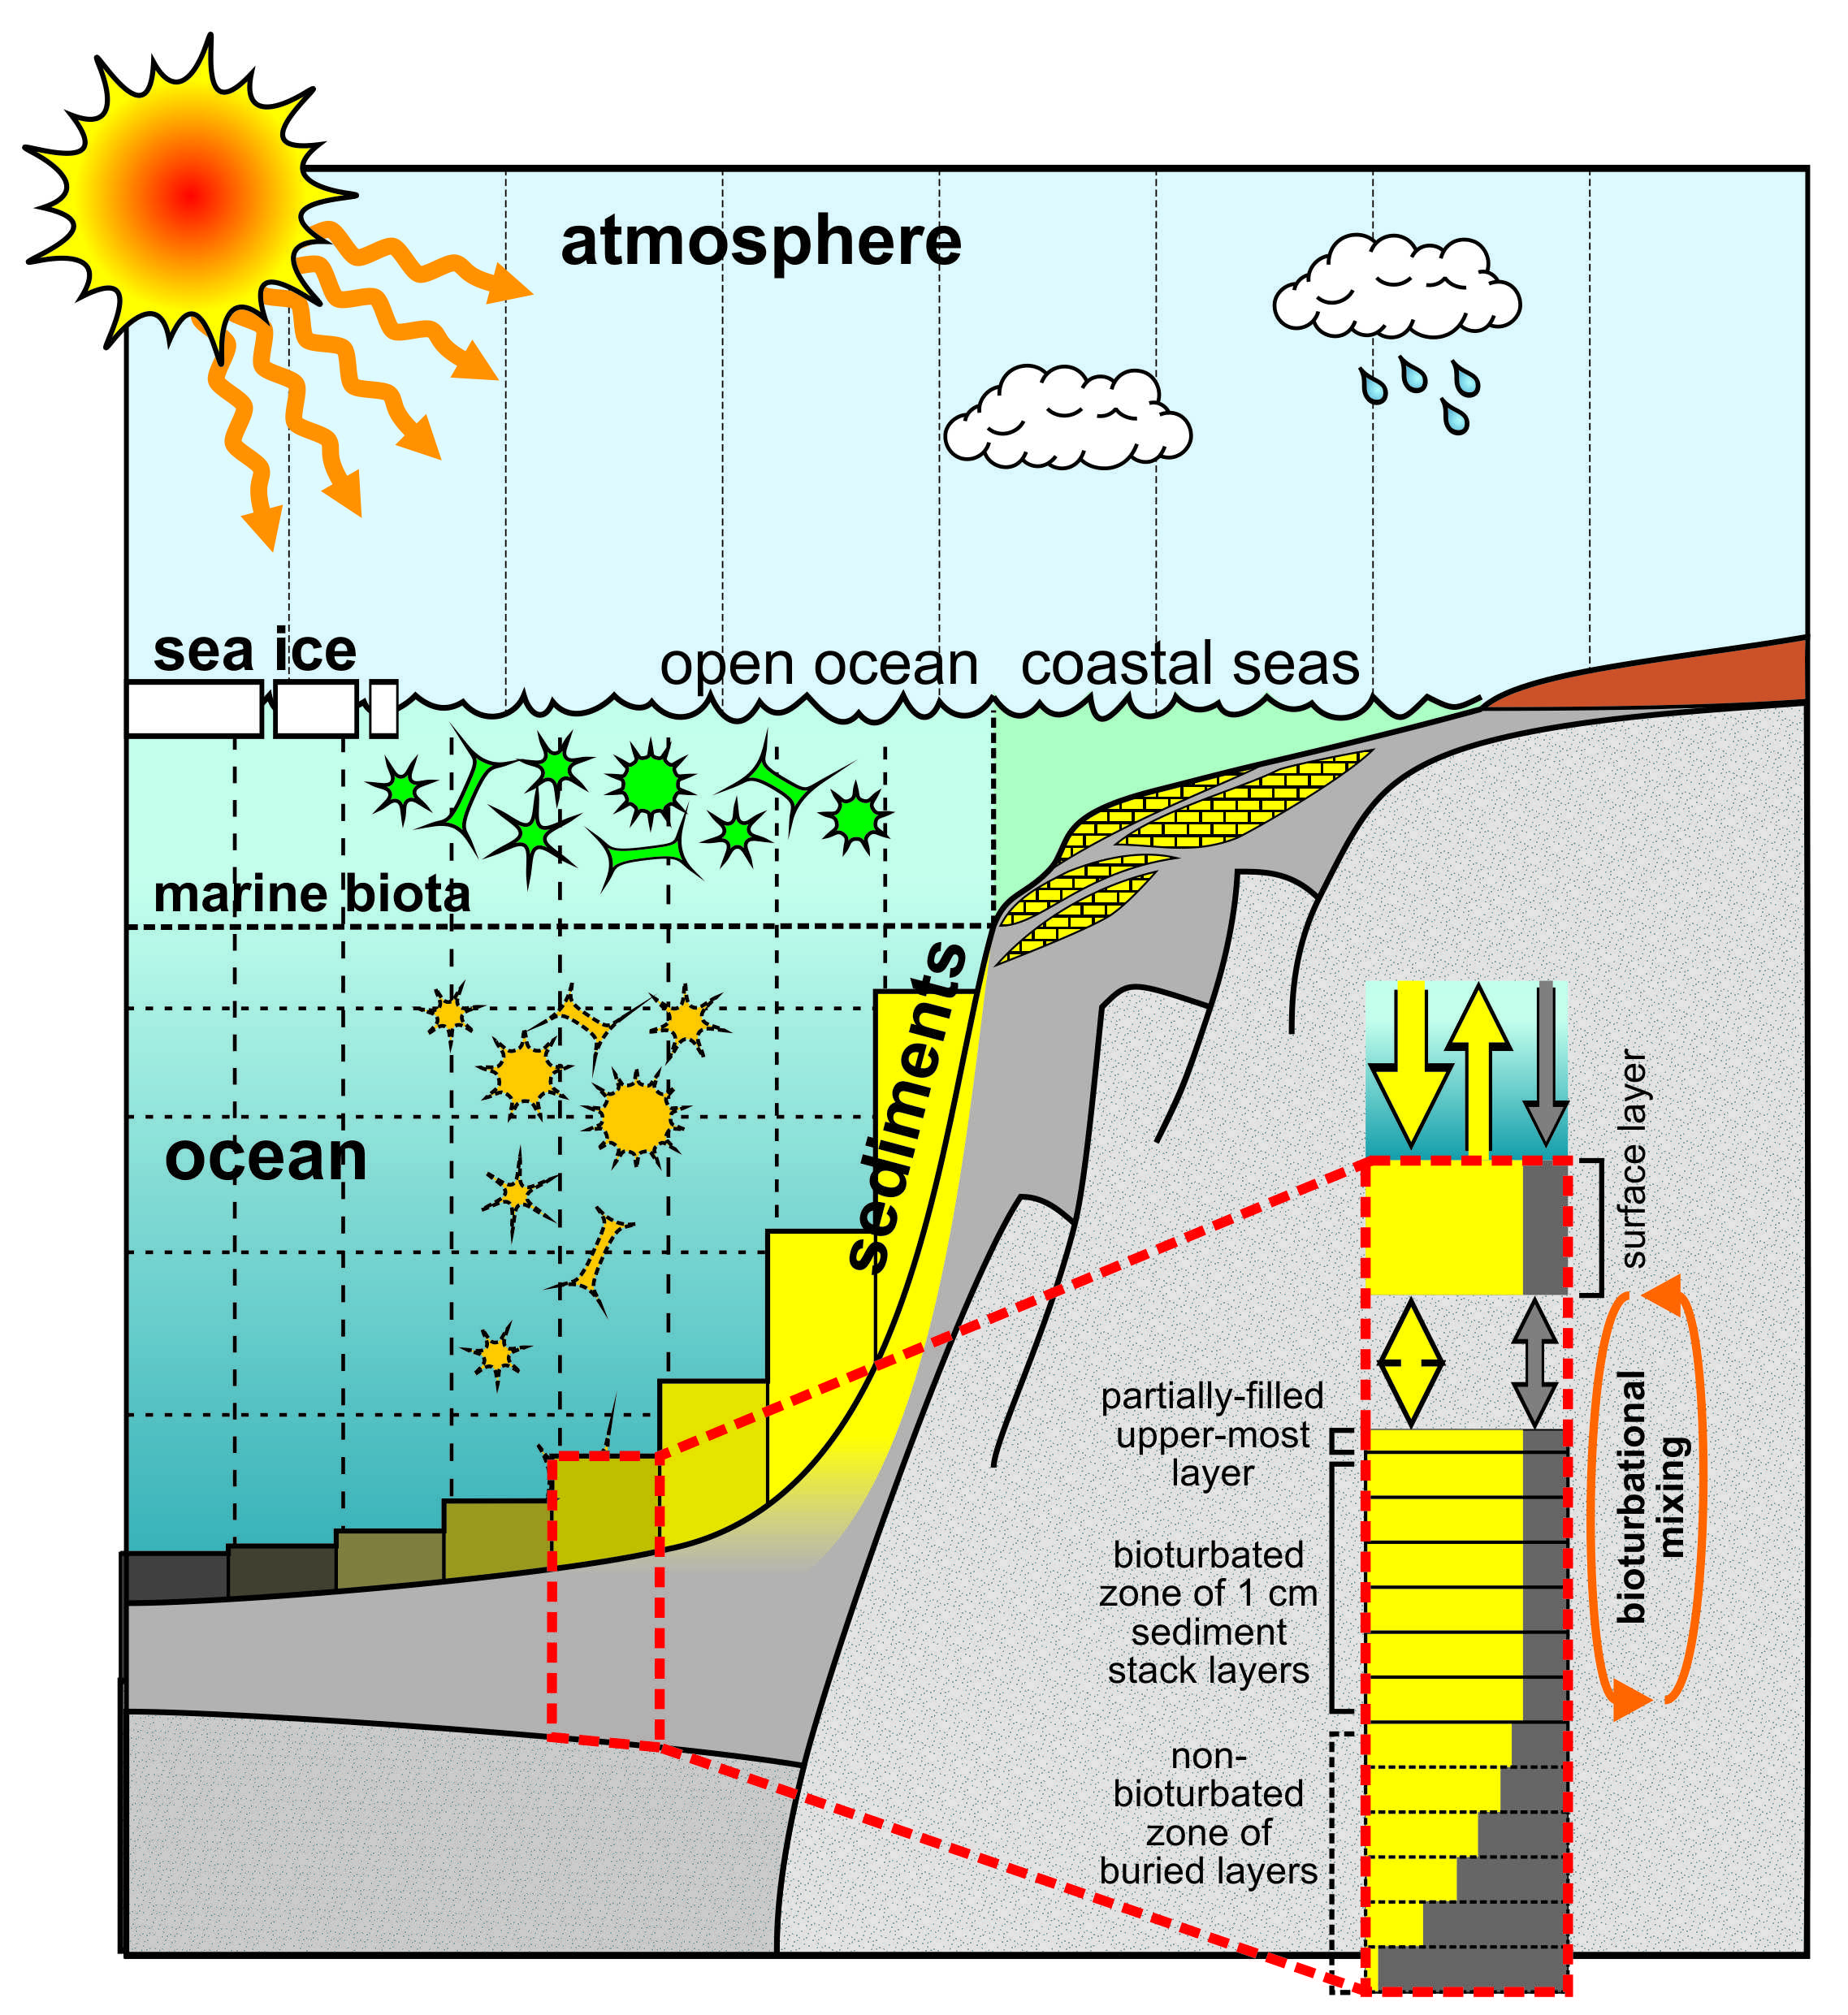
\includegraphics[width=0.5\textwidth]{sediments.jpg}
\caption{Schematic of SEDGEM sediment component.}
\label{fig:sediments}
\end{figure}

%------------------------------------------------

\section{Sediment model output}

There is a whole new set of additional outputs from this configuration of cGENIE, including sediment output (from the ‘SEDGEM’ module). For instance, the composition of the sediments only at the very end of a model experiment (hence unlike BIOGEM, which saves a series of time-slices long) is saved by the SEDGEM module – kill a run before this, and you will get no (or little) output. 2D (e.g. surface sediment properties) results can be found in the sedgem subdirectory of your experiment directory and in a netCDF file called fields\_sedgem\_2d.nc. (Note that there is some duplication of results saving, because a series of time-slices of sediment composition are also saved in the 2D biogem netCDF file fields\_biogem\_2d.nc alongside with sea-ice extent etc.). The time-series file: biogem\_series\_sed\_CaCO3.res also contains information about how the mean CaCO3 content of surface sediments evolves with time.

For instance, the 2D distribution of wt\% CaCO3 – which is the weight fraction of calcium carbonate (CaCO3) in the surface sediments of the deep ocean (i.e., how much plankton carbonate shell material is there compared to other stuff in the mud at the bottom of the ocean?) is saved under a variable called: sed\_CaCO3. How much carbonate material there is tells you both something about how many carbonate shell secreting plankton were living at the ocean surface above and what is the chemistry of the deep ocean like that these tiny shells were preserved and did not dissolve. To gauge to what degree the faster configuration of cGENIE might provide an adequate representation of the interaction between ocean chemistry and sediment composition (e.g., in CaCO3 buffering of \(CO_{2}\) release and 'carbonate compensation'), the output should be contrasted to observational-based maps as well as (higher resolution) model results (e.g., as presented by Ridgwell and Hargreaves [2007]). Appreciate that cGENIE does not reproduce reality ... particularly at this lower resolution, but does it get the broad patterns right (is it more right than wrong, or more wrong than right)? Do you think the model-data misfits might be important? (Note that there is a reconstruction of the glacial pattern of CaCO3 in sediments that is available and may be of use in constraining your glacial \(CO_{2}\) hypothesis, or at least testing it against data.)

\vspace{1mm}
\noindent\rule{4cm}{0.1mm}
\vspace{2mm}

The model also generates artificial sediment ‘cores’ (e.g. see: Ridgwell [2007]) and hence what one might expect to see of your applied perturbations recorded in a sediment core recovered from the ocean floor. In the sedgem results sub-directory, there is a netCDF file which contains all the locations selected (if any) – sedcore.nc. These are not really aligned with latitude as the Panoply display might suggest – the locations are in fact distributed from all over the ocean (Panoply is being fooled in order to display them together). In the SEDGEM 2D netCDF file, these locations are marked in the netCDF variable grid\_mask\_sedcore. The locations of these cores are stored in a little ASCII ‘map’ of the ocean in the directory:

\begin{verbatim}
~/cgenie.muffin/genie-sedgem/data/input
\end{verbatim}

and the file for this experiment is given by the parameter: sg\_par\_sedcore\_save\_mask\_name
Simply be editing (using the ASCII text editor) a ‘0.0’ to a ‘1.0’, you can get the model to generate and save a sediment ‘core’ at that location.

The sedcore.nc. variables are displayed as a function of ‘latitude’. Variables include:

•       phys\_layer – sediment layer number (counting down).
•       phys\_depth – (cumulative) depth below surface, measured from the sediment surface to the mid-point of each sediment layer (cm).
•       th (cm) – thickness of each sediment layer (cm).
•       age\_CaCO3 – the mean age of CaCO3 particles in a sediment layer. Note that this will not be defined if there is no CaCO3 preserved.
•       … then some alternative ways of assigning a chronology to a sediment core … (ignore).
•       phys\_porosity – sediment layer density (as if you cared!).
•       sed\_POC and sed\_POC\_13C – mean organic matter content of each sediment layer and its \(d13C\)\. But note: in this configuration no organic matter is preserved (hence all zeros for POC).
•       sed\_CaCO3 and sed\_CaCO3\_13C – mean CaCO3 content (wt%) of each sediment layer and its 13C.
•       sed\_det and sed\_ash – the wt\% detrital and ‘ash’ contents of a layer (ash is used as a conservative numerical sediment tracer in order to mark the depth of the start of the experiment).

Obviously – you could plot e.g. CaCO3 (or its \(\delta^{13}C\)) as a function of depth and/or age across and see how your carbon release experiment might be recorded in the marine geological record. How does this compare with e.g. the PETM?
Note that the sediment cores reflect not only the material which has accumulated (or not, if it has dissolved …) during the course of your experiment, but also the material that accumulated during the 50,000 year spin-up. AND, whatever material the sediment core was initialized with to start with. The large interval of first 100\% detrital material below which everything is zero simply reflects the initialization of the sediment array in the model. Also note the ash ‘peak’ near the bottom of the stack (filled) sediment layers – this is a tracer to ‘tag’ the start of the model spin-up. If you look at the spin-up results (not your recent perturbation experiment) – the ash peak lies in a sediment layer with age 50,000 years. But why is there any ash deeper than the age corresponding to the start of the spin-up? How can it get there?

%------------------------------------------------

\newpage

%------------------------------------------------

\section{Further ideas}

You can also explore the role of weathering and sensitivity of e.g. atmospheric \(pCO_{2}\) and climate to this (as well as to volcanic \(CO_{2}\) outgassing). Because the time-scale for seeing interesting stuff happen is now going to be l o n g … you need some help.

The \textit{user-config} file: \texttt{LAB\_x.weathering} is provided which uses a ‘trick’ to accelerate the run-time (the new section \texttt{\# --- GEOCHEM ACCELERATION ---}) … see Lord et al. [2015]. 

Parameters if ‘interest’ that might be adjusted in the context of weathering and long-term controls on atmospheric \(pCO_{2}\) (listed under \texttt{\# --- WEATHERING ---}), include:

\begin{itemize}[noitemsep]
\item \texttt{rg\_par\_outgas\_\(CO_{2}\)} -– \(CO_{2}\) outgassing rate in mol yr-1
\item \texttt{rg\_par\_ref\_T0} -– reference land surface temperature for weathering (C)
\end{itemize}

\vspace{1mm}
\noindent\rule{4cm}{0.1mm}
\vspace{2mm}

\noindent You might investigate other facets of the nature of the relationship between ocean and sediments (and weathering) as how climatic (biogeochemical) signals are encoded in the marine geological record. For instance, you could explore the effect/importance of sediment ‘bioturbation’ (e.g. see \textit{Ridgwell} [2007]). Whether the surface sediment layers are bioturbation or not is set by the parameter:
\begin{verbatim}
sg_ctrl_sed_bioturb=.true.
\end{verbatim}
Simply change to \texttt{.false.} in order to ‘turn off’ bioturbation.

\vspace{1mm}
\noindent\rule{4cm}{0.1mm}
\vspace{2mm}

Rather than driving an initial dissolution of CaCO3 in deep sea sediments, the opposite (initial response) can be obtained by removing \(CO_{2}\) from the atmosphere (implemented by negative rather than positive emissions). BE CAREFUL here, as for a pre-industrial atmosphere with 278 ppm \(CO_{2}\), you do not have a lot more than \~600 PgC in there to begin with. So either: remove less than 600 PgC, or remove the carbon over a little longer than 1 year – implement this either by editing the forcing files directly, or set a scaling parameter for the duration.

(Hint: a forcing for removing \(CO_{2}\) simply has the opposite sign to an addition (emissions) forcing.)

Again – view the time-series of ocean composition (e.g. DIC, ALK, \(d13C\)) as a function of time, plus mean sediment surface composition (wt\% CaCO3). Also view the sediment ‘cores’ and hence what in practice has been incorporated into accumulating sediments as a record of what is a very sharp perturbation at the ocean surface (and atmosphere).

How then is an event characterized by \(CO_{2}\) removal from the system recorded differently from one characterized by \(CO_{2}\) release? Are there different implications for constructing core age-scales and chronology, e.g. where in (core) ‘time’ does the excursion maximum appear to lie? Do all sediment locations show identical responses (i.e. does it matter what the initial wt\% CaCO3 is?).

%----------------------------------------------------------------------------------------
%       CHAPTER X
%----------------------------------------------------------------------------------------

\cleardoublepage

\chapterimage{13750210193_e161c3ede1_b.jpg} % Chapter heading image

\chapter{Geological processes II}

\hfill \break

\vspace{18mm}

\noindent Stuff to keep in mind:
\hfill \break

\noindent "\textit{There are known knowns.\\
These are things we know that we know.\\
There are known unknowns.\\
That is to say, there are things that we know we don't know.\\
But there are also unknown unknowns.\\
There are things we don't know we don't know.}"

\hfill \break
\noindent Donald Rumsfeld, former US Secretary of Defense

%------------------------------------------------

\newpage

%------------------------------------------------

\section{README}

blah

%------------------------------------------------

\newpage

%------------------------------------------------

\section{How low can you go?}

Your task is to explain low glacial atmospheric CO2.

It is up to you whether you aim for ~190 ppm, or want to retain as much consistency with other (paleoceanographic) constraints as possible.

In addition to the control and spin-up user-configs, you have been provided with: exp12\_glacial which can be used as a template user-config file for you to base (if you want!) your glacial CO2 investigations on (at least initially).

\vspace{1mm}
\noindent\rule{4cm}{0.5pt}
\vspace{2mm}

Before embarking upon some glacial experiments (below) – other model outputs/fields you might
also keep in mind and for which some data/observational constraints on your glacial CO2 'solution'
may be available (e.g. see Kohfeld and Ridgwell [2009]), include:

\begin{itemize}
        \item 
The 2D fields\_biogem\_2d.nc field: phys\_seaice ('sea-ice cover'), for which some glacial
sea-ice limit information exists. (CLIMAP)
        \item 
The 2D fields\_biogem\_2d.nc field: ocn\_sur\_temp ('surface-water temp') (or view the
surface ocean layer in the 3D file), for which 2 (one older, one newer) comprehensive
datasets exists -- it would be reasonable to question whether you achieve an adequate
glacial (surface) climate state and if not, whether this impacts any bias (and in which
direction) to your CO2 solution. (CLIMAP, MARGO)
        \item 
The 2D fields\_biogem\_2d.nc field: sed\_CaCO3 ('sediment core-top CaCO3') (also
available from the sedgem model output), for which some glacial CaCO3 distribution
data/estimates exist. (Old Catubig paper in GBC)
        \item 
The 2D fields\_biogem\_2d.nc field: phys\_opsia (' Atlantic streamfunction'). While poorly
resolved in this model configuration, many (glacial) model studies report the circulation field
and hence they provide a point of comparison for your GENIE-based research.
        \item 
The 2D fields\_biogem\_2d.nc field: ocn\_D\_DIC\_13C (' planktic-benthic difference
DIC\_13C') and also the individual planktic (surface) and benthic (bottom) fields. A
significant amount of d13C data exists in the literature for both glacial and interglacial states.
        \item 
The 2D fields\_biogem\_2d.nc field: ocn\_ben\_O2 (' bottom-water O2') (and also horizontal
slices in the 3D file). Ideally, no-where in the ocean should anoxia (no oxygen) occur. It
certainly should not be widespread across one or more ocean basins if your glacial CO2
solution is to get published in Nature ;)
        \item 
The 2D fields\_biogem\_2d.nc field: ocn\_ben\_sal ('bottom-water sal') (and also in the 3D
file as horizontal slices), for which some estimates exists for a few places in the ocean.
(Jess Atkins Science paper)
        \item 
The 2D fields for surface and deep PO4 (and also in the 3D file as horizontal slices) as
some proxy evidence exists for changes in nutrient utilization. (Cd/Ca proxies – e.g. papers
by Elderfield and Rickaby)

\end{itemize}

Also refer to the 3D netCDF files and the time-series where helpful.

Note here that the spin-up provided is 'modern' and hence glacial data cannot be directly
contrasted -- the above suggestions/guidance are intended as a starting point only.

\vspace{1mm}
\noindent\rule{4cm}{0.5pt}
\vspace{2mm}

In your glacial CO2 investigations, 2 separate initial modifications of the model will nudge it in the
vague direction of a glacial state (e.g., see Kohfeld and Ridgwell [2009]):

\begin{itemize}[noitemsep]

\item A modification of surface (actually 'planetary') albedo to try and take account of some of the
cooling influences of the large (Northern Hemisphere) ice sheets that were present during
the last glacial but which are not calculated or explicitly taken into account in the version of
cGENIE you are using.

\item A modification of greenhouse gas radiative forcing (as per in the snowball Earth
experiments) to take into account the lower CO2, CH4, and N2O concentrations in the
atmosphere during the last glacial. While you will be attempting to reproduce ca. 190 ppm
atmospheric CO2 (and hence deduce the reasons for low glacial CO2), you may not
necessarily achieve this, and you have no means of explicitly controlling the other
A Hitchhikers Guide to the advanced Black Arts (of Earth system modelling)
LAB Session VII
3
greenhouse gases, so you may as well get the radiative forcing and hence the glacial
climate state as close as possible before trying to adjust the carbon cycle. But it is up to you
whether you prefer to not 'cheat' and have whatever CO2 cGENIE simulates, directly affect
climate (and hence feed back on CO2).
\end{itemize}

The glacial boundary conditions are implemented as follows:

\begin{itemize}[noitemsep]

\item To achieve a pseudo-glacial planetary albedo modification, add the following lines to a
user-config file (and see Lab V):
\vspace{-1mm}\begin{verbatim}
# adjusted planetary albedo
ea_albedop_offs=0.200
ea_albedop_amp=0.360
ea_albedop_skew=0.0
ea_albedop_skewp=4
ea_albedop_mod2=-15.000
ea_albedop_mod4=-2.500
ea_albedop_mod6=0.000
\end{verbatim}\vspace{-1mm}

\item For glacial radiative forcing, add the lines:
\vspace{-1mm}\begin{verbatim}
# glacial CO2 radiative forcing
ea_radfor_scl_co2=0.6835
# glacial CH4 radiative forcing
ea_radfor_scl_ch4=0.5
# glacial N2O radiative forcing
ea_radfor_scl_n2o=0.8
\end{verbatim}\vspace{-1mm}

\end{itemize}

If you like – you can carry out separate experiments to test the effect of each of these in turn and
hence to learn the effect and impact on atmospheric CO2 of each individually before combining
them. Ideally, these lines should ultimately be included in all (glacial) experiments that you require
glacial albedo and radiative forcing for.

By all means play around with the albedo and radiative forcing climate boundary conditions,
although one might wonder the reasoning behind adjusting radiative forcing below e.g. that
appropriate for full glacial conditions. However, the planetary albedo is less certain as implemented
in the model. For instance, one might legitimately adjust this to achieve appropriate last glacial sea
surface temperatures (SST), or rather: a glacial-interglacial difference in SSTs similar between
model and data.

\vspace{1mm}
\noindent\rule{4cm}{0.5pt}
\vspace{2mm}

By this point, you should have created a new (mostly) spun-up model state, incorporating: (i)
higher planetary albedo, and (ii) lower greenhouse gas forcing. The duration of this new, glacial
spin-up needs to be sufficient to bring the system into (a new) equilibrium (of which the slowest
adjusting component will be sediment composition (wt% CaCO3), although continuing changes in
wt\% CaCO3 will to some extent be reflected in continuing changes in pCO2 (why?)).

Before carrying on, check that everything is 'correct' (or at least: understandable) so-far. In
particular: confirm that you have a colder ocean (due to altered albedo and/or greenhouse
radiation forcing) ... no, seriously! You never know what might have gone wrong with a simple slip
of the keyboard ... Surface ocean temperature also has established proxies for its glacial value and
so the model can be contrasted against data.

The file biogem\_series\_ocn\_temp.res is the time-series results file for ocean temperature – the
2nd column is the mean ocean temperature, the 3rd column is mean sea surface temperature
(SST), and the 4th mean benthic (deep (> 2 km) ocean floor). How much colder has it become? Is
this realistic? Analyze the SST distribution (the surface field of the 3D netCDF time-slice file, or the
'sur\_*' variables in the 2D netCDF file) – how does this compare to observations? In the book
chapter the data-based difference in SST between the LGM and Holocene is given. However, the
map given is for the glacial-interglacial difference, which happily is something you have previously
learned to do using Panoply (I hope!).

Also, what is the CO2 impact of lower SSTs? Note that you may not be able to directly compare
your CO2 prediction with all previous studies (e.g. summarized in the book chapter) because in
your model, sea-ice and ocean circulation will also have been affected to some extent by the
climate change. (How much have they been affected? There are also some proxies for sea-ice
extent as well as ideas and hypotheses about ocean circulation changes.) Many (but not all)previous model studies have simply estimated CO2 changes due to temperature change with fixed
sea-ice and circulation fixed, by prescribing a different ocean surface temperature for the CO2
solubility calculation. (This is a little beyond the scope of what you are expected to do here, but can
be done in GENIE.)

\vspace{1mm}
\noindent\rule{4cm}{0.5pt}
\vspace{2mm}

Unless you are *extremely* lucky and already have a value of atmospheric CO2 that is 90 ppm
lower than pre-industrial (ca. 278 ppm) ... (WTF?!) – you may want to test other changes that might
have taken place between glacials and interglacials that affected CO2. Obviously a spot of creating
new user-config files will be in order here (perhaps using: exp12\_glacial as a template, but it is
entirely up to you). Ideally, you would test the impact of each change individually first before
combining them, so as to develop a better understanding of the different ways in which CO2 is
controlled (and the associated impacts on other elements of the global carbon cycle and climate)
before bunging everything in together.

Before diving straight in -- note the number of different modifications of the global carbon cycle that
might be considered and tested in the model. What is your methodological strategy going to be?
Are you going to add all of the modifications into a single run and hope that you can understand
what has happened at the end? (I hope not!) Are you going to run all the modifications individually
(how?). Are you going to try combinations to test whether any combine non-linearly? You will want
to make use of the cluster queue and submit at least some of the experiments. You will also need t
already have a good idea of how long to run them before (hopefully you obtained this knowledge
from the idealized perturbation experiments in the previous tutorials).

Some suggestions (i.e., this not an exhaustive list, nor a prescribed one and not everything
necessarily has to be done!):

%------------------------------------------------
%
\subsection{Global weathering rate.}

Refer to Ridgwell and Zeebe [2005] for the role of weathering.
Also to Kohfeld and Ridgwell [2009] for some references to the changes in weathering that
might have taken place between glacial and interglacial. The namelist parameter that
controls the annual rate of solute input into the ocean is:

rg\_par\_weather\_CaCO3=0.9E+13

Either edit this value (under heading: \# --- WEATHERING ---) or add a new line at the
end of the user config file specifying the value you want. Units are mol of CaCO3 weathered
per year.

This parameter could also be adjusted to implicitly simulate the effect of a change in
carbonate deposition in coral reefs and other shallow water carbonates, changes that
GENIE cannot simulate explicitly. See Ridgwell et al. [2003]

(http://www.seao2.org/pubs/ridgwell\_et\_al\_2003a.pdf) for references and discussion of the
sort of change in carbonate deposition on the shelves that might have taken place. A
decrease in CaCO3 removal on the continental shelves can be simulated by increasing the
weathering flux to the open ocean. In other words, you can look at the parameter
rg\_par\_weather\_CaCO3 as representing the residual weathering flux to the open ocean,
after some of the weathering flux has been removed in coastal areas. Even if global
weathering of the continents did not change, any reduction in CaCO3 precipitation and
removal on the continental shelves would result in an increased solute flux to the open
ocean.

[HINT: keeping track of how mean sediment wt\% CaCO3 changes will be helpful, as may
2D sediment dist
ributions and ultimately, the sediment core records.]

%------------------------------------------------
%
\subsection{Iron fertilization.}

Read up on this first, e.g., see references in Kohfeld and Ridgwell [2009].
The glacial was dustier than present, hence there can only have been increased aeolian
iron supply to the ocean surface. However, what is not so clear is how important (relative to
Fe being upwelled) aeolian Fe is today, let alone during the last glacial ...

Anyway: one way to increase the aeolian Fe supply to the ocean surface is simply to
increase the solubility of the Fe in dust. This is controlled by the parameter:

bg\_par\_det\_Fe\_sol=0.0015

with the default being a global average dust Fe solubility of 0.15% (fraction == 0.0015).
Increasing will increase the Fe input to the ocean surface everywhere (in direct proportion
to the modern spatial pattern). The pattern of total aeolian Fe supply is recorded in the (2DBIOGEM) variable: 

misc\_sur\_fFetot\_mol, with the dissolved component under:

misc\_sur\_fFe\_mol (misc\_sur\_Fe\_sol is the map of solubility, which in GENIE is not
uniform in space -- any idea what the reason for this assumption might be?).
(A glacially-explicit map of dust deposition could also be applied in place of the modern
deposition map -- if you would like to test this, I can create one, but note that there are very
significant 'errors' in re-gridding dust maps to this highly simplified continental topography.)

[HINT: viewing maps of particulate organic carbon (POC) export may be particularly
helpful.]

%------------------------------------------------
%
\subsection{Remineralization depth.}

There is no temperature control on the rate of bacterial
degradation of sinking organic matter (see: book chapter + references therein) but the
effect of lower ocean temperatures and a slower rate of bacterial degradation of organic
matter can be simulated by specifying that particulate organic matter reaches greater depth
before being remineralized (and CO2 and PO4 released back to the seawater). The namelist
parameter that controls the e-folding depth reached by particulate organic matter before
remineralization is:

bg\_par\_bio\_remin\_POC\_eL1=589.9451

Either edit this value (under heading: \# --- REMINERALIZATION ---) or add a new line at
the end of the user config file specifying the value you want. Units are m.
Read Ridgwell et al. [2007] for additional discussion of this parameter. See Figure 2-4 in
Ridgwell [2001] (http://www.seao2.org/pubs/ridgwell\_thesis.pdf) for an illustration of how
the flux of particulate organic matter decreases with depth in the ocean, plus references
therein.

There is also an associated parameter: bg\_par\_bio\_remin\_POC\_frac2, which sets a
fraction of organic matter that is assumed to settling through the water column completely
un-altered (currently assigned a value of 0.025 == 2.5\%), but this is arguably less
appropriate to change than the remineralization length-scale of the more labile fraction
(97.5\% of exported particulate organic carbon).

[HINT: viewing distributions of PO4 and/or O2 in the ocean may be helpful. Perhaps also
d13C.]

%------------------------------------------------
%
\subsection{Macro nutrient inventory and uptake.}

Suggestions have been made that nutrients were
used more efficiently during the LGM, meaning that for the same nutrient uptake at the
surface more carbon was exported to depth in the ocean. See: Omta et al. [2006]. There
are also a bunch of (relatively old) hypotheses concerning differences between glacial and
modern ocean in how much nitrate (NO3
-) there was. There is no NO3
- in this version of
GENIE (just PO4
3- and Fe), but an analogous change can be made to the phosphorous
cycle.

For the nutrient-to-carbon ratio in organic matter, the relevant parameter is:

bg\_par\_bio\_red\_POP\_POC=106.0

To change the default value (106.0), add a new line at the end of the user-config file
specifying the value you want. A larger number means that PO4 is being utilized more
efficiently and more organic matter ir being produced for the same nutrient consumption.

If you would like to test the effect of adding more PO4 to the (glacial) ocean -- a forcing is
provided, called:

p0000b\_FeMahowald2006\_ADJUST\_phosphate

Note that adjusting the ocean PO4 inventory should only be done one (and not accidentally
in each successive experiment!).

[HINT: viewing distributions of PO4 and/or O2 in the ocean may be helpful. Also ocean
sediment CaCO3 distributions.]

%------------------------------------------------
%
\subsection{CaCO3:POC rain ratio.}

Kicked off by a classic 1994 Nature paper by Archer and Maier-
Reimer (see: Kohfeld and Ridgwell [2009]), one powerful means of changing atmospheric
CO2 that has been proposed involves changes in the export ratio between CaCO3 (shells)
and POC (particulate organic matter). Such a change in ratio could come about through a
variety of ways (e.g., via the 'silica leakage hypothesis' (see: Kohfeld and Ridgwell [2009])
and also through the direct effect of Fe on diatom physiology (see Watson et al. [2000] in
Nature and also Supplemental Information). There are also ideas about an opposite ocean
acidification effect, whereby the less acidic glacial (compared to modern) ocean led to
increased calcification and CaCO3 export. Note that this response (higher saturation ==
great calcification) is encoded into your model configuration – see Ridgwell et al. [2007b].

In GENIE, the CaCO3:POC rain ratio is controlled (technically: scaled) by the parameter:

bg\_par\_bio\_red\_POC\_CaCO3=0.03

The pattern of CaCO3:POC rain ratio is not uniform across the ocean (why? (see: Ridgwell
et al. [2007, 2009]), and its pattern can be viewed in the (2D BIOGEM) netCDF variable:

misc\_sur\_rCaCO3toPOC.

[HINT: viewing sediment CaCO3 distribution may be helpful.]

%------------------------------------------------
%
\subsection{Sea-ice extent.}

Changes to sea-ice extent have already taken place due to changes in
radiative forcing and planetary albedo (made previously). There is no much you can do to
further adjust sea-ice extent, other than via further changes to climate (via radiative forcing
and/or albedo).

%------------------------------------------------
%
\subsection{Atlantic circulation.}

There are a variety of ideas and hypotheses about glacial ocean
circulation and what influence it had on atmospheric CO2. At least with respect to making
tests and experiments in models, a common ploy has been to produce a collapsed AMOC
(e.g., see Chikamoto et al. [2008] (JGR 113)). Rather than apply a continuous freshwater
forcing to the ocean throughout an extended (sediment interaction) time-scale (why would
this not be a good idea?), there is a parameter in the model which creates an adjustment of
the salt balance between the different ocean basins (to make the Atlantic more salty
compared to the Pacific). (In other words: salt/freshwater is re-partitioned between the
ocean basins rather than 'new' freshwater or salt externally added.) This parameter is:

ea\_28=0.726862013339996340

Setting it to e.g., 0.0, will result in a collapsed AMOC. But maybe that is too extreme? (You
might read up a little on the glacial ocean circulation literature and chose a value that gives
as an appropriate change to Atlantic circulation as you can judge from the data and
literature.)

[HINT: viewing distributions of PO4 and/or O2 and/or d13C in the ocean may be helpful. Also
ocean sediment CaCO3 distributions.]

%------------------------------------------------
%
\subsection{Global ocean circulation / 'brine rejection'.}

Some recent research has focussed on the
possible role of 'brine rejection' in creating a saltier Antarctic bottom waters (e.g. see Adkins
et al. 2002 Science paper) and hence a denser and more stratified deep ocean,, with the
idea being this will trap carbon more efficiently. For a very recent study (and references
therein), see:

http://www.clim-past.net/6/575/2010/cp-6-575-2010.html

GENIE has the capability to include this effect (at least crudely) and similarly to Bouttes et
al. [2010]. For this, three namelist parameter values need to be set:

\vspace{-2mm}\begin{verbatim}
bg_ctrl_force_GOLDSTEInTS=.TRUE.
bg_par_misc_brinerejection_frac=0.1
bg_par_misc_brinerejection_jmax=9
\end{verbatim}\vspace{-2mm}

The first, simply allows the BIOGEM biogeochem module to directly influence ocean
circulation. The second is the fraction of salt, rejected during sea-ice formation (e.g., see
Bouttes et al. [2010]) that is transferred directly to the bottom-most (underlying) ocean cell
in the model. The first sets a latitude limit (counted in cells) to the effect -- a value of 9 will
restrict brine rejection to the Southern Ocean; a value of 18 will allow it to take place in the
North Atlantic as well. (Note that in e.g., Bouttes et al. [2010], the effect is considered only
in the Southern Ocean.)

[HINT: viewing distributions of PO4 and/or O2 and/or d13C in the ocean may be helpful. Also
ocean sediment CaCO3 distributions.]

%------------------------------------------------
%
\subsection*{MISC.}

There are of course other possibilities for adjusting the model, although you need an
a priori reason for doing so and what about the possible glacial state of global carbon
cycling and climate you are trying to encapsulate. Examples might include wind speed (or
air-sea gas exchange).

\vspace{1mm}
\noindent\rule{4cm}{0.5pt}
\vspace{2mm}

Even if you achieve atmospheric CO2 of ca. 190 ppm (and actually, with some mechanisms on
their own and also in combination, it is quite easy to achieve this), how do you know if you are ‘right’? Many of the important constraints are summarized in Kohfeld and Ridgwell [2009] and
Archer et al. [2000]. In particular:

\begin{itemize}[noitemsep]

\item 
The distribution of the CaCO3 content of deep-sea sediments. e.g., see Figure 6 in Archer
et al. [2000]. You are not ‘allowed’ to blanket the entire ocean floor with CaCO3 if you want
to be consistent with the paleoceanographic record of the LGM ;)

The predicted distribution of the CaCO3 can be used to assess your circulation change –
note that there is much less CaCO3 in sediments in the North Atlantic at the glacial [Archer
et al., 2000]. See: Chikamoto et al. [2008] for a model assessment of the impact of AMOC
changes on deep-sea sediment composition.

\item 
The ocean should not go ‘anoxic’ (i.e., little to no dissolved oxygen left) over large
expanses. (But you might consider this relative to the modern configuration – i.e., should
the modern simulation under-estimate oxygen concentrations in the deep ocean, so will the
glacial simulation, even if you get the mechanisms exactly 'right'.)

\item 
There is a map of estimated changes in the biological flux to the ocean floor in Kohfeld and
Ridgwell [2009] (also read the original reference). In the 2D netCDF file, the variable
focnsed\_POC gives you the flux of particulate organic matter (actually, carbon) to the ocean
floor. By constructing a difference map of your glacial-interglacial predicted changes, you
could contrast directly to the Kohfeld et al. [2005] reconstruction.

\item 
The GENIE model is set up to predict d13C distributions. See: Curry and Oppo [2005].
There is also an atmospheric record of d13C (also predicted by GENIE) – see: Smith et al.
[1999] and a more recent paper in GBC: Lourantou et al. [2010] ('Constraint of the CO2 rise
by new atmospheric carbon isotopic measurements during the last deglaciation ').

\item Other proxies offer varying constraints at the global or regional scales. e.g., see: Elderfield
and Rickaby [2000] (Cd/Ca ratios).

\end{itemize}

Note that commonly in (glacial CO2) modeling studies, a steady state (or quasi steady state)
simulation is run for the glacial (and compared to pre-indsutrial). The version of cGENIE you have
is sufficiently fast to do this quite effectively. It is possible to do non-state (glacial-interglacial)
simulations, e.g. Ridgwell [2001], but this is rather more involved.

Also note that in all of the above possible adjustments to the global carbon cycle, the mechanism
of carbonate compensation is operating. Hence there will be direct (changes in carbon cycling
within the water column) and indirect (interaction between ocean and deep-sea sediments)
processes operating that will affect CO2. Carbonate compensation will typically take a few 10s of
thousands of years to fully adjust atmospheric CO2. Not all previous modeling studies include this
effect and in some cases it can drastically influence the predicted change in atmospheric CO2.

\vspace{1mm}
\noindent\rule{4cm}{0.5pt}
\vspace{2mm}

Finally … maybe you have achieved close to 190 ppm and are not unreasonably consistent with
various paleoceanographic proxies and are hence feeling rather pleased with yourself … O -- sorry -- I forget to mention a little something:

\begin{itemize}[noitemsep]
\setlength{\itemindent}{.2in}
\item 
There is as approximately 3\% (1 PSU) increase in salinity (and other dissolved tracers)
due to the presence of large (Northern Hemisphere) ice sheets, and hence loss of
freshwater from the ocean and lower sea-level associated with the last glacial.
\end{itemize}

\noindent Ahhhh … and I also forgot:

\begin{itemize}[noitemsep]
\setlength{\itemindent}{.2in}
\item It is thought that there was a release of carbon stored on land in vegetation and soils during
glacial climates. (cGENIE has some capabilities to model changes in terrestrial carbon
storage and hence predict this, but you are not using a version with this science module
enabled.)
\end{itemize}

Unfortunately – both these effects act to increase atmospheric pCO2 at the last glacial (or decrease
it across the deglacial transition, which ever way around you like to think of it). So you are actually
rather further off achieving a net 90 ppm difference than you thought.

%------------------------------------------------
%
\subsection{Salinity}

To test the effect of a 3\% increase in salinity at the last glacial, you need to create a new userconfig
file (copied from your last glacial ‘best guess’ configuration), add the lines:
\vspace{-2mm}\begin{verbatim}
bg_ctrl_force_GOLDSTEInTS=.true.
bg_par_forcing_name=’p0000b_FeMahowald2006_ADJUST_salinity’
\end{verbatim}\vspace{-2mm}
and run using your last glacial best guess as the restart.

If you want to check that you have applied this forcing correctly: Mean ocean salinity should end higher than the preindustrial restart that was
originally provided (or compared to your best guess glacial run). The file
biogem\_series\_ocn\_sal.res is the time-series results file for ocean salinity – the 2nd
column is the mean ocean salinity. Originally it was 34.904 PSU (or o/oo), now it should be
about 35.9.

Note how atmospheric pCO2 has responded to the change in ocean volume and sea-level
(and tracer concentrations) alone. How does this reduced resolution version of cGENIE
compare to published estimates (too much; too little; why? or if

%------------------------------------------------
%
\subsection{Terrestrial carbon storage}

For the reduction in terrestrial carbon storage, you need to try a further experiment (on top of
and/or following on from the salinity change experiment), with the user-config line:

bg\_par\_forcing\_name=’p0000b\_FeMahowald2006\_ADJUST\_terrestrialC’

These two forcings are effectively one-off changes imposed on the global climate and carbon
cycle. By selecting the salinity forcing, you add 1 PSU of salinity to the entire ocean (and
concentrate proportionally all dissolved tracers in the ocean) in a single year. Obviously you only
want to do this once, not multiple times (other wise you will get an increasingly salty ocean ...).
Similarly with the terrestrial carbon change – as specified, this forcing results in 500 PgC of carbon
being added to the atmosphere over a period of 500 years (i.e., at a rate of 1 PgC yr-1) as if to
simulate a commensurate reduction in carbon stored on land. One strategy might be to implement
this as a second phase of (additional) spin-up (after the salinity modification). Note that while the
magnitude of the glacial-interglacial salinity and sea-level change is well constrained, that of the
terrestrial biosphere is not (e.g., see: Kohfeld and Ridgwell [2009]). In investigating the potential
causes of low glacial CO2, do not feel constrained to necessarily run with the default (500 PgC)
forcing provided ... (Think for yourselves!)

To confirm that you have correctly added (rather than subtracted!) carbon to the ocean+
atmosphere -- thee ocean + atmosphere carbon inventories should start changing from the
start of the experiment incorporating the carbon change forcing

(p0000b\_FeMahowald2006\_ADJUST\_terrestrialC)

and the change should be
approximately uniform. You can calculate the change in ocean + atmosphere carbon
inventory from the atmospheric CO2 time-series file (biogem\_series\_atm\_pCO2.res --
column \#2 is the global CO2 inventory in mol) and the ocean total dissolved carbon timeseries
file (biogem\_series\_ocn\_DIC.res – column \#2 is the global DIC (total dissolved
inorganic carbon) inventory in mol). Note you will have to convert from mol to gC (or PgC)
in order to compare to the amount you requested. If the rate of inventory change turns out
to be not quite linear, and particularly if the inventory change should turn to be not quite
what you were expecting ... why? (Hint: refer to the mechanisms discussed in the lecture
(and papers) relating deep-sea sediments and weathering to changes in total carbon (e.g.,
fossil fuel CO2 release.)

\begin{figure}
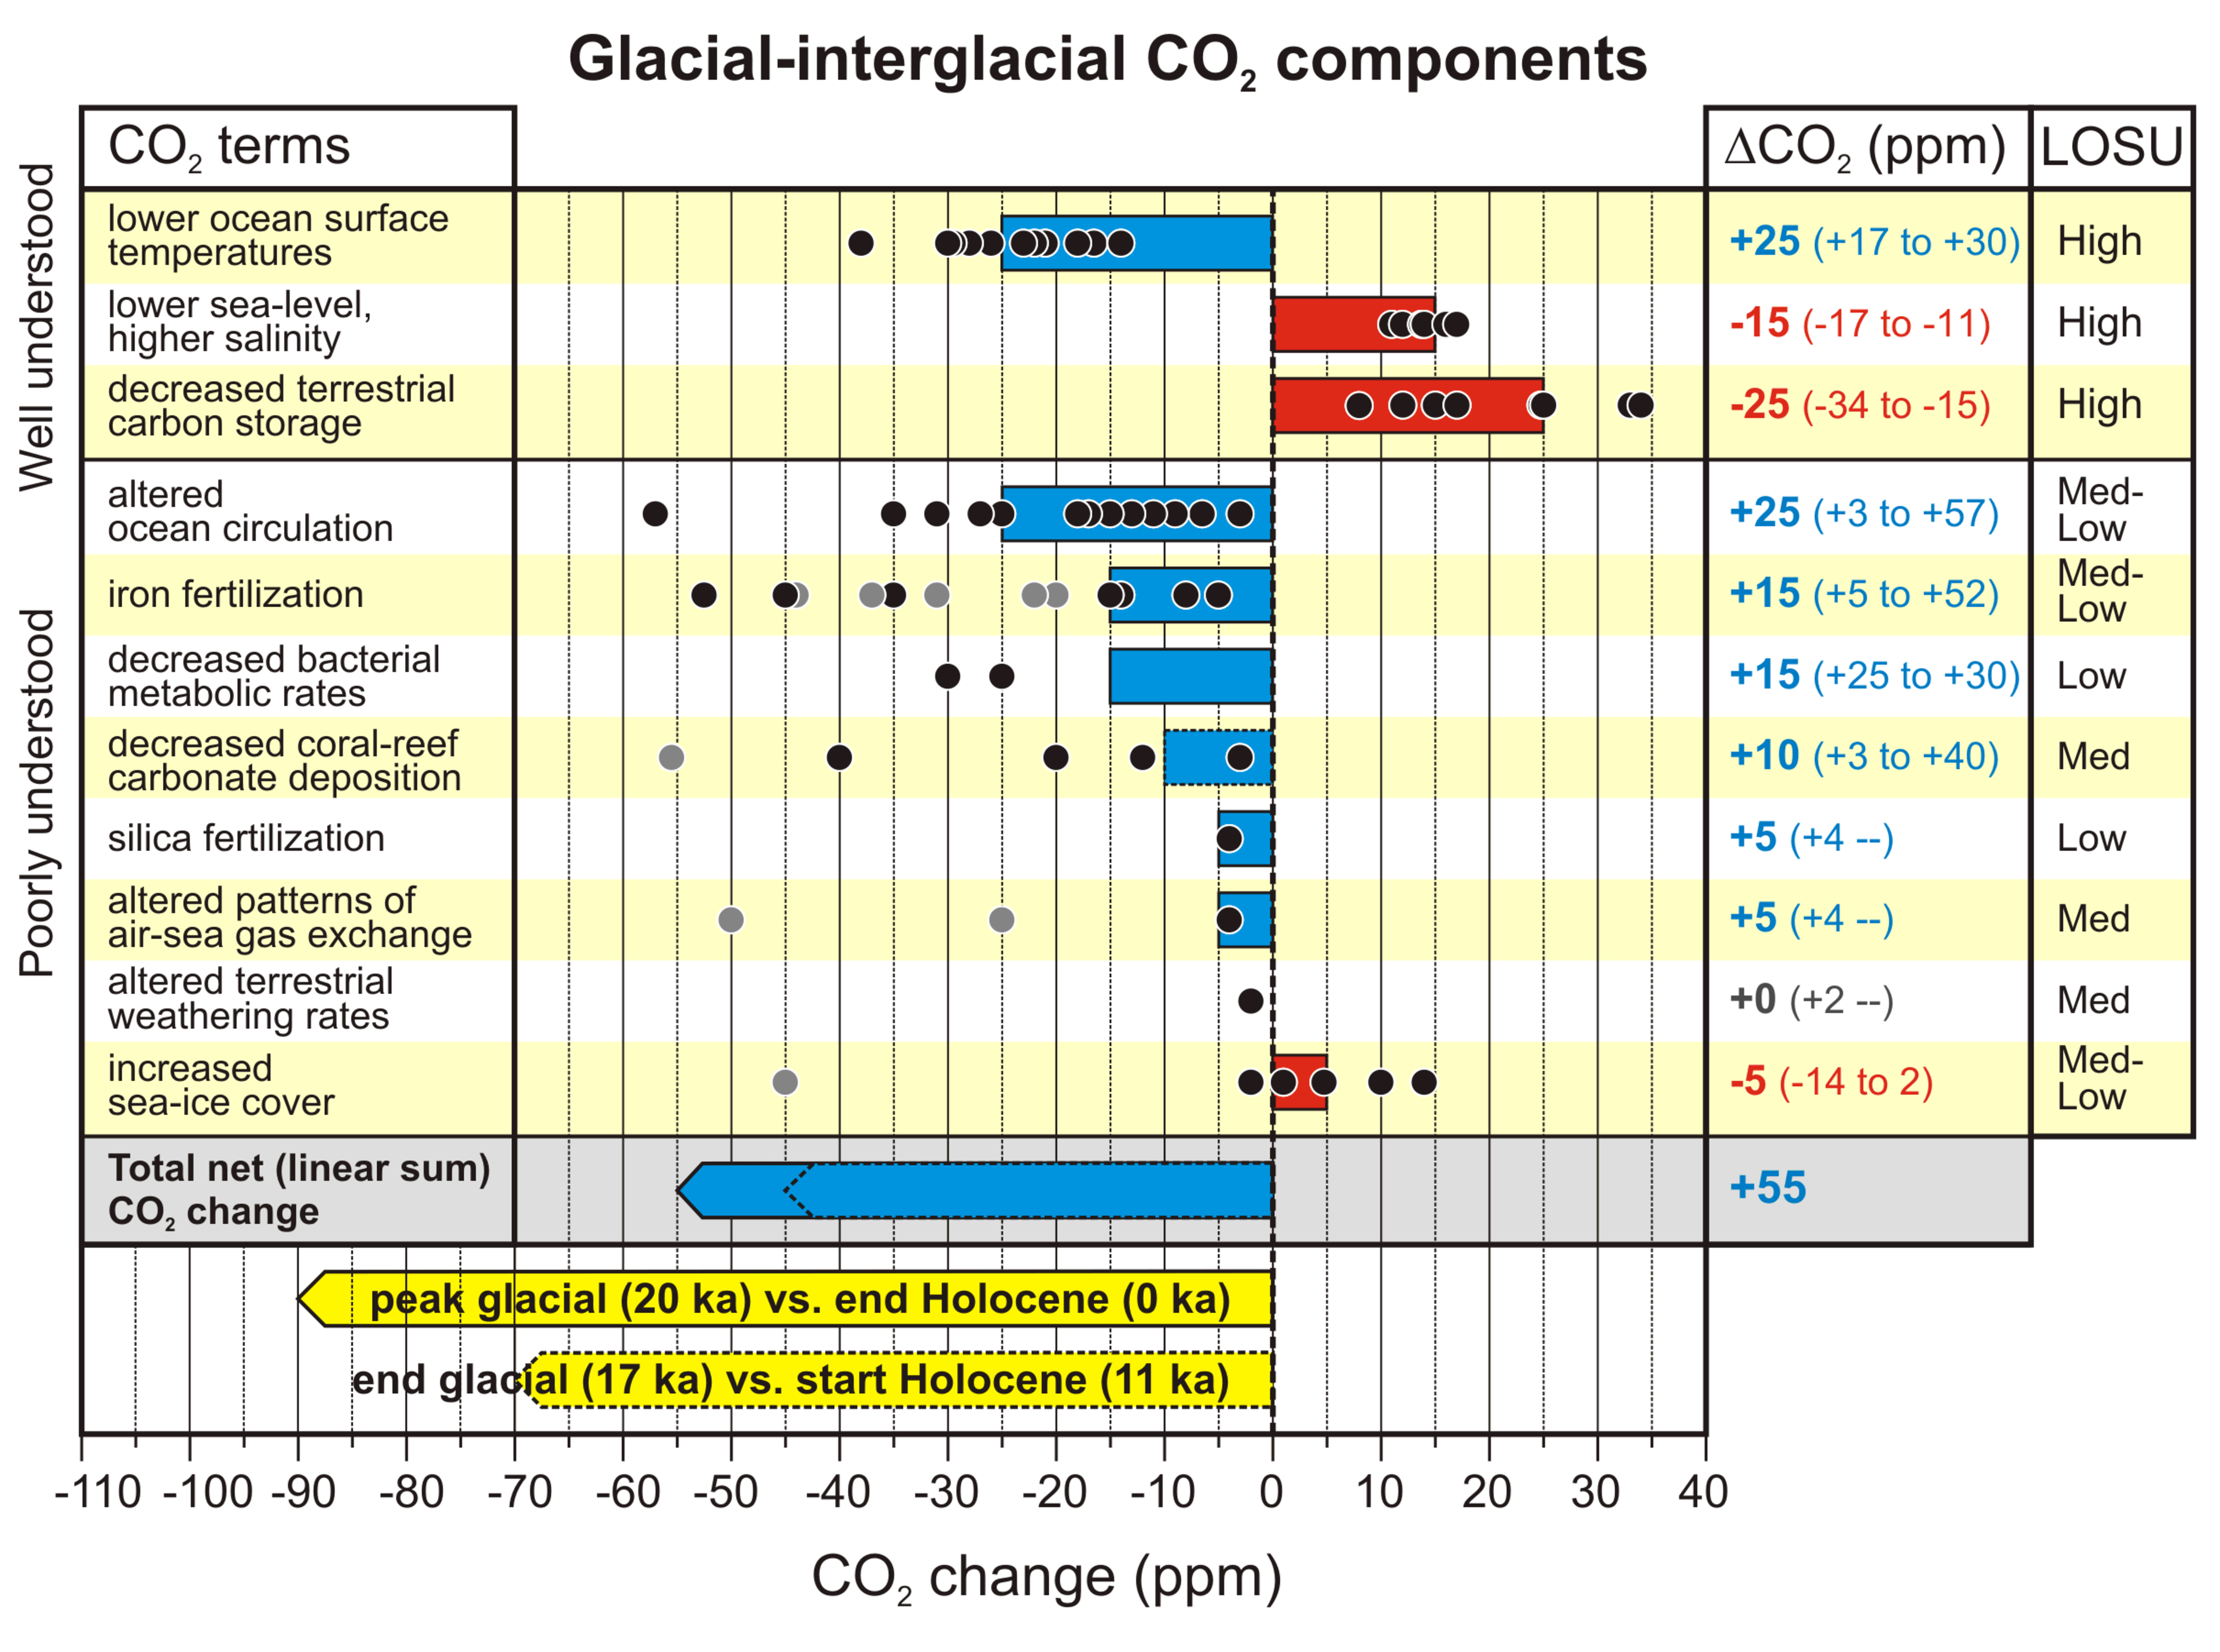
\includegraphics[width=1.00\textwidth]{CO2_components_110104.gif}
\caption{Baaaa.}
\label{fig:sediments}
\end{figure}

%----------------------------------------------------------------------------------------
%       CHAPTER X
%----------------------------------------------------------------------------------------

\cleardoublepage

\chapterimage{nSTnj.jpg} % Chapter heading image

\chapter{muffin model output}

\hfill \break

\vspace{24mm}

\noindent This section covers \textbf{muffin} saves data and how to ensure that the variables you want are saved and when you want.

\begin{itemize}
        \item Overview.
        \item \textit{Time-series} output.
        \begin{itemize}
                \item \textit{Time-series} file naming conventions.
                \item Specifying frequency and timing of \textit{time-series} data saving.
                \item Seasonal/monthly data saving.
        \end{itemize}
        \item \textit{Time-slice} output.
        \begin{itemize}
                \item \textit{Time-slice} file naming conventions.
                \item Specifying frequency and timing of \textit{time-slice} data saving.
        \end{itemize}
        \item Specifying which data fields to be saved in the \textit{time-series} and \textit{time-slice} format.
        \item \textit{Re-start} files.
\end{itemize}

%------------------------------------------------

\newpage

%------------------------------------------------

\section{Overview (and types of model output)}

The results of experiments are written to the directory:
\begin{verbatim}~/cgenie_output\end{verbatim}
For any particular experiment, all saved model results, plus copies of input parameters and the model executable, are gathered together in a directory that is assigned the same name as the experiment (== \textit{user-config} file name), e.g.:
\begin{verbatim}EXAMPLE.worbe2.Ridgwelletal2007.SPIN\end{verbatim}
Every science module saves its results in its own individual sub-directory within the experiment directory. So for the module that calculates ocean biogeochemical cycles -- \textbf{BIOGEM}, the results files will thus be found in:
\begin{verbatim}~/cgenie_output/EXAMPLE.worbe2.Ridgwelletal2007.SPIN/biogem\end{verbatim}
Note that \textbf{ATCHEM} does not save its own results (\textbf{BIOGEM} can save information about atmospheric composition and air-sea gas exchange) while \textbf{SEDGEM} essentially saves results only at the very end of a model experiment (\textbf{BIOGEM} can also save the spatial distribution of sediment composition as time-slices as well as mean composition as a time-series). Furthermore, in order to attain a common format for both ocean physical properties and biogeochemistry, \textbf{BIOGEM} can save a range of ocean results in addition to temperature and salinity, such as: velocities, sea-ice extent, mixed layer depth, convective frequency, etc. Also note that \textbf{SEDGEM} saves data only at the end of an experiment\footnote{With the exception of sediment core location environmental properties, which are saved more frequently.}.

Saving full spatial distributions for any or all of the tracers at each and every time-step is not practical, not only in terms of data storage but also because of the detrimental effect that repeated disk access has on model performance. Instead, \textbf{BIOGEM} saves the full spatial distribution of whatever tracer, flux, and/or physical properties of the system are required (how what fields are required is specified is discussed later), only at one or more predefined time points (in years). These are called '\textit{time-slices}'. However, rather than taking an instantaneous snapshot, the time-slice is constructed as an average over a specified integration interval.
The second main data format for model output is that of a '\textit{time-series}' of change in a single (integrated) property of the Earth system. Model characteristics must be reducible to a single meaningful variable for this to be practical (i.e., saving the time-varying nature of 3-D ocean tracer distributions is not). Suitable reduced indicators include: the total inventories in the ocean and/or atmosphere of various tracers (or equivalently, the mean global concentrations / partial pressures, respectively), global sea-ice coverage. Like \textit{time-slices}, the data values saved in the \textit{time-series} files represent averages over a specified integration interval (one year by default). For both \textit{time-slices} and \textit{time-series} output, the files themselves are created during model initialization and are periodically updated (appended to) during the experiment. Hence, even before the experiment has finished they may contain data that is useful to view and can be used to check on the progress of an experiment.

\subsubsection{ATCHEM}

\noindent In the \textbf{ATCHEM} results directory, only the following file will be present:

\begin{enumerate}

\vspace{1mm}\item \texttt{\_restart.nc} -- \textit{Re-start} file -- a snap-shot of the 2D distribution of atmospheric composition at the very end of the experiment. Not intended for user-access, although it can be plotted just like any normal \textit{netCDF} format file.

\end{enumerate}\vspace{2mm}

\subsubsection{BIOGEM}

\noindent For \textbf{BIOGEM}, some or all of the following files will be present:

\begin{enumerate}

\vspace{1mm}\item \texttt{\_restart.nc} -- \textit{Re-start} file -- a snap-shot of the 3D distribution of biogeochemical properties of the ocean at the very end of the experiment. Not intended for user-access, although it can be plotted just like any normal \textit{netCDF} format file.

\vspace{1mm}\item \texttt{fields\_biogem\_2d.nc} -- 2-D fields of (mostly) ocean bottom, ocean surface, and sediment surface properties.\footnote{The mid-points at which time-slices are saved are specified as described above.} Also: water-column integrals of certain geochemistry diagnostics, air-sea gas exchange fluxes, atmospheric composition.

\vspace{1mm}\item \texttt{fields\_biogem\_3d.nc} -- 3-D fields ocean dissolved and particulate tracer properties.\footnote{The mid-points at which time-slices are saved are specified as described above.}

\vspace{1mm}\item \texttt{biogem\_series\_*.res}\footnote{\texttt{.res} is a useful format for processing in \textbf{MATLAB}; for other programs, other extensions are needed. If using the Mathematica data processing scripts - see \texttt{genie-docs/cGENIE.AutomationScripts} - \texttt{.dat} is needed; this can be set with  \texttt{gm\_string\_results\_ext=".dat"}} -- \textit{Time-series} results files -- globally and surface-averaged (and sometimes also benthic (bottom) surface averaged) property values as a function of time in plain text (ASCII) format.

\vspace{1mm}\item \texttt{biogem\_year\_*\_diag\_GLOBAL.res} -- Miscellaneous global diagnostic information. It is saved at each requested time-slice with the file-name string containing the mid-point of the time-slice (as years). The diagnostics include:
        \begin{itemize}
                \item time mid-point and integration interval
                \item global ocean surface area and volume
                \item mean global sir-sea gas exchange coefficient (for CO\begin{math}_2\end{math})
                \item mean atmospheric tracer concentrations plus total inventory
                \item mean ocean tracer concentrations plus total inventory
                \item mean plus total global productivity
                \item mean plus total global sedimentation
        \end{itemize}
        
\end{enumerate}\vspace{2mm}

\subsubsection{SEDGEM}

\noindent In the \textbf{SEDGEM} results directory, some or all of the following files will be written:

\begin{enumerate}

\vspace{1mm}\item \texttt{\_restart.nc} -- \textit{Re-start} file -- a snap-shot of the 2D distribution of sedimentary properties at the very end of the experiment. Not intended for user-access, although it can be plotted just like any normal \textit{netCDF} format file.

\vspace{1mm}\item \texttt{fields\_sedgem\_2d.nc} -- Contains 2-D fields of sediment surface and ocean bottom properties.\footnote{This data is saved only at the termination of an experiment (i.e., the \textit{netCDF} file contains only a single time-slice).}

\vspace{1mm}\item \texttt{sedcore.nc} -- \textit{netCDF} format file containing the stacked records of accumulated deep-sea sediment composition.
\\The locations (if any) of sediment cores to be saved is specified in a plain text (ASCII) file pointed to by the string value of the \textit{namelist} parameter \texttt{sg\_par\_sedcore\_save\_mask\_name}\footnote{The location of this file is specified by the \textbf{SEDGEM} data input directory namelist parameter: \texttt{sg\_par\_indir\_name} which by default is \texttt{\~{}/genie-sedgem/data/input}.}. In the mask file, a '\texttt{1}' indicates a location to save a sediment core at, and a '\texttt{0}' indicates that no sediment core should be saved at this location.       This file must be present, so to save no sediment cores, simply populate the file with all zeros in an \texttt{xx} by \texttt{yy} grid.

\vspace{1mm}\item \texttt{sedcoreenv\_*} -- These files contain pseudo time-series of surface sediment environmental properties at each of the requested sediment core locations (if any are chosen).

\vspace{1mm}\item \texttt{seddiag\_misc\_DATA\_GLOBAL.res} -- A summary of mean global sedimentation, dissolution, and preservation fluxes, and surface sediment composition.

\vspace{1mm}\item \texttt{seddiag\_misc\_DATA\_FULL.res} -- Surface sediment and bottom water properties at each and every sediment grid point.

\end{enumerate}\vspace{2mm}

\subsubsection{ROKGEM}

\noindent In the \textbf{ROKGEM} results directory, some or all of the following files will be written:

\begin{enumerate}

\vspace{1mm}\item \texttt{fields\_rokgem\_2d.nc} -- 2-D fields of (mostly) land surface, ocean surface, and atmospheric properties related to weathering.

\vspace{1mm}\item \texttt{biogem\_series\_*} -- Time-series results files.
        
\end{enumerate}\vspace{2mm}

%------------------------------------------------

\newpage

%------------------------------------------------

\section{\textit{Time-slice} output}

%------------------------------------------------

\subsection{Frequency and timing of \textit{time-slice} data saving}

Rather than taking an instantaneous snapshot, the time-slice is averaged over a specified integration interval \begin{math}\Delta t\end{math} (in years), defined by the parameter \texttt{bg\_par\_data\_save\_slice\_dt}\footnote{An empty list is valid - time-slices will then be populated for you at an interval set by the time-slice integration interval. But if you really don't want any time-slices, just set the first (or only) time point to occur beyond the end year of the run.}. The model state is thus integrated from time \begin{math}t_{n} - \Delta t/2\end{math} to \begin{math}t_{n} + \Delta t/2\end{math}. For instance, setting a value of \begin{math}\Delta t = 1.0\end{math} year results in all seasonal variability being removed from the saved time-slices, and successive time-slices then only reflect long-term (\textgreater 1 year) trends in system state.

\vspace{1mm}The mid-point years (\begin{math}t_{n}\end{math}) for which time-slices should be saved are specified in a single column pain text (ASCII) file in the \texttt{cgenie.muffin/genie-biogem/data/input} directory, whose name is specified by the parameter \texttt{bg\_par\_infile\_slice\_name}\footnote{The location of this file is specified by the \textbf{BIOGEM} data input directory parameter: \texttt{bg\_par\_indir\_name} which by default is \texttt{\~{}/genie-biogem/data/input}.}.
For example, the default \textit{time-slice} specification file \texttt{save\_timeslice.dat} contains the specification\footnote{The order in which the time sequence is ordered (i.e., ascending or descending time values) does not actually matter in practice as long as the list of times is ordered sequentially. The list will be internally re-ordered if necessary according to the selection of ‘BP’ (the model running backwards-in-time) or not according to the logical value of the parameter \texttt{bg\_ctrl\_misc\_t\_BP}, which is \texttt{.false.} by default.}:
\footnotesize\begin{verbatim}
-START-OF-DATA-
0.5
1.5
4.5
9.5
19.5
49.5
99.5
199.5
499.5
999.5
1999.5
4999.5
9999.5
19999.5
49999.5
99999.5
199999.5
499999.5
999999.5
-END-OF-DATA-
\end{verbatim}\normalsize
where \texttt{-START-OF-DATA-} and \texttt{-END-OF-DATA-} are simply tags delineating the start and end of the time point data.
Use of this particular specification lends itself to simple experiment run durations to be adopted (e.g., 10, 100, 10000 years). It provides a good generic starting point in that save frequency is faster to begin with (when environmental variables are more likely to be rapidly changing) and less frequently later (when environmental variables are unlikely to be changing rapidly and maybe converging to steady-state).

To change the time points used for \textit{time-slice} data saving, either direct edit this file (less good), or create a new file (e.g. simply copy and rename \texttt{save\_timeslice.dat}) with the required save frequency and timing and saved to the \texttt{cgenie.muffin/genie-biogem/data/input} directory, with the parameter \texttt{bg\_par\_infile\_slice\_name} pointing to the new filename).

%------------------------------------------------

\subsection{Experiment end saving}


Just in case an experiment run duration is chosen such that there is no corresponding save point anywhere near the end of the run, a \textit{time-slice} is automatically saved at the very end of an experiment regardless of whether one has been specified or not and with the same averaging as used for the specified \textit{time-slices}.

%------------------------------------------------
%
\subsection{Seasonal/monthly data saving}

\textit{Time-slice} (but not currently \textit{time-series}) data can be saved seasonal or even monthly by selected by setting a single parameter rather than e.g. specifying a monthly or seasonal data save interval and editing the time-slice definition file with a series of min-points for months (or seasons).
The way it works is that the overall averaging interval (parameter: \texttt{bg\_par\_data\_save\_slice\_dt})\footnote{Default value = 999} is broken down into sub-intervals of averaging. i.e., breaking down a year interval (the default) into 4 will give seasonal averaging. The parameter: \texttt{bg\_par\_data\_save\_slice\_n} where \textit{n} sets the number of time steps in each sub-interval of data saving and hence determines whether the averaging is e.g. seasonal or monthly. The slightly tricky part is to be sure of how many time steps in each year ;) 

By default, \textbf{\textit{c}GENIE.muffin} employs 96 time-steps per year for a 16-level ocean circulation model (\textbf{GOLDSTEIN}) and 48 for \textbf{BIOGEM}\footnote{Note that when running using \texttt{runmuffin.t100.sh}, 100 time-steps are taken in the ocean and 50 in BIOGEM for a 16 level ocean model.}. Hence for a 16-level ocean configuration, seasonal data saving would be obtained with:
\begin{verbatim}bg_par_data_save_slice_n=12\end{verbatim}
(12 \textbf{BIOGEM} steps per averaging interval out of a total of 48), and monthly averages with:
\begin{verbatim}bg_par_data_save_slice_n=4\end{verbatim}
(i.e. 4 \textbf{BIOGEM} steps for each of the 12 monthly averaging intervals, giving of a total of 48).

For lower resolution configurations of \textbf{\textit{c}GENIE.muffin}, \textbf{GOLDSTEIN} may be operating on 48 time-steps per year, and \textbf{BIOGEM} on 24 or even 12. As \textbf{\textit{c}GENIE.muffin} starts up it will report the ocean and biogeochemical time-stepping, such as:
\small\begin{verbatim}
>> Configuring ...
   Setting time-stepping [GOLDSTEIN, BIOGEM:GOLDSTEIN]:  100 2
\end{verbatim}\normalsize
which specifies 100 time-steps per year for \textbf{GOLDSTEIN}, and 50 per year (100/2) for \textbf{BIOGEM} for the case of a 16 level ocean using the \texttt{runmuffin.t100.sh} run script.
Note that for every year mid-point specified in the\textit{ time-slice} specification file, 4 or 12 (for seasonal and monthly, respectively) times as many time-slices will actually be saved.

%------------------------------------------------
%
\subsection{More frequent data saving}

Explicit frequent saving of fields or properties at specific locations can be done by setting a more higher save frequency of the time-slice data. However, because the 2D and 3D fields may contain a variety of unwanted variables in addition to the target one, save frequency is likely to be limited by the maximum netCDF file size that can sanely be manipulated. The practical maximum is around 100, depending on the number of types of data field selected to be saved. Several alternative options are available:

\begin{itemize}
\item (trivial) Make do with global or surface (or benthic) means in the time-series output.
\item Cut down the types of data saved to the absolute minimum (see 'Data field selection' below).
\item Save only 2D data. This can be accomplished by setting the parameter:
\vspace{-1mm}\begin{verbatim}
bg_ctrl_data_save_2d=.true.
bg_ctrl_data_save_3d=.false.
\end{verbatim}\vspace{-1mm}
(both are \texttt{.true.} by default). This disables the 3D data saving, although an empty netCDF file will still be created.
\item Save the tracer fields in 3D, but at the save frequency of time-series data saving\footnote{This is in addition to normal 3D saving at the time-slice data saving frequency}. This can be done by setting:
\vspace{-1mm}\begin{verbatim}
bg_ctrl_data_save_3d_sig=.true.
\end{verbatim}\vspace{-1mm}
(by default, \texttt{.false.}).
\end{itemize}

%------------------------------------------------

\newpage

%------------------------------------------------

\section{\textit{Time-series} output}

%------------------------------------------------

\subsection{Frequency and timing of \textit{time-series} data saving}

For results \textit{time-series}, a file containing a series of model times (\begin{math}t_{n}\end{math}) at which data points need be saved is defined in the same way as for \textit{time-slices}, with the filename specified by the parameter \texttt{bg\_par\_infile\_sig\_name}. Again, the data values saved in the time-series file do not represent discrete values in time but an average, calculated from time \begin{math}t_{n} - \Delta t/2\end{math} to \begin{math}t_{n} + \Delta t/2\end{math} as per the construction of time-slices. The averaging interval, \begin{math}\Delta t\end{math}, is set by the value of the parameter \texttt{bg\_par\_data\_save\_sig\_dt}. The format is also identical to before (with tags delineating the start and end of the list of mid-points). If there are less than two elements present in the list, a default frequency of data saving will be invoked, set equal the averaging interval, except in the situation that this results in an unreasonably large amount of data, when an order of magnitude (or more than one order of magnitude where necessary) fewer save points are assumed.\footnote{For historical reasons ... the maximum number of time-series (and time-slice) data points was set to 4096. This is set by the parameter \texttt{n\_data\_max} in \texttt{biogem\_lib.f90} and can be altered if required.} The default setting:
\small\begin{verbatim}bg_par_infile_sig_name='save_timeseries.dat'\end{verbatim}\normalsize
provides for reasonably generic data saving, with the save frequency faster to begin with and becoming progressively less frequently later.

There is a related facility to \texttt{bg\_par\_infile\_sig\_name} for \textbf{SEDGEM} and \textbf{ROKGEM} in the parameter: \texttt{xx\_par\_output\_years\_file\_0d}, where \texttt{xx} is \texttt{sg} for \textbf{SEDGEM} and \texttt{rg} for \textbf{ROKGEM}. These specify files in the \texttt{genie-*gem/data/input} directory and again contain a list of years for 0D (time-series) output to be generated at. However, unlike \textbf{BIOGEM}, the data saved \textit{do} represent discrete values in time and \textit{not} e.g. annual averages.

%------------------------------------------------

\subsection{Saving orbital insolation}

[see orbits HOW-TO]

%------------------------------------------------

\newpage

%------------------------------------------------

\section{Data field selection}

Model output -- both \textit{time-slice} and \textit{time-series} data are saved in blocks or  by categories of model variables. For instance, all dissolved tracers in the ocean (3D netCDF \textit{time-slice} and/or \textit{time-series}), or all particle flux fields, all carbonate chemistry and associated variables, all surface sediment composition, etc etc. This still requires a multitude of parameters, one for each category and generally also one for each of \textit{time-slice} and \textit{time-series} data. In an attempt to simplify this, a single parameter, \texttt{bg\_par\_data\_save\_level}, specifying the sort and amount of data to save can be set instead.

The value of the \texttt{bg\_par\_data\_save\_level} save level parameter is given as an integer between \texttt{0} and \texttt{99}, and has the following effect:

\vspace{2mm}\begin{itemize}

\item[0] -- Save nothing.
\item[1] -- Minimum -- basic geochemistry only, i.e. ocean and atmosphere tracer fields (omitting e.g. the miscellaneous fields and time-series -- see below).
\item[2] -- Basic output == basic geochemistry and physics.
\item[3] -- Basic + biology diagnostics, i.e. ocean and atmosphere tracer fields plus particulate  flux fields and biological diagnostics such as limitations on export.
\item[4] -- Basic + geochemistry diagnostics, including output on air-sea gas exchange, ocean carbonate chemistry, and geochemical diagnostics such as remineralization rates and transformation, ocean pH field (3D), Fe cycle and speciation diagnostics (2D). In conjunction with the \textbf{ROKGEM} module, also: weathering fluxes.\footnote{The most common option.} \item[5] -- Basic + biology + geochemistry diagnostics. A combination of \texttt{3} and \texttt{4}.
\item[6] -- Basic + tracer diagnostics. Tracer diagnostics includes: N*, P* etc., water column inventories (2D).
\item[7] -- Basic + tracer + proxy diagnostics. Proxy diagnostics includes: ocean surface and benthic (and surface-benthic) tracers (2D). Also trace metals (e.g. Cd).
\item[8] -- Basic output + biology + geochemistry + tracer + proxy diagnostics.
\item[9] -- Basic output + full physics (e.g. all grid specifications and properties).
\item[10] -- Ocean acidification option == basic geochemical output fields plus all carbonate chemistry.
\item[99] -- Save everything.
\item[>99] -- Use explicit user-specified settings for individual save categories. This is the default and is broadly consistent with previous version of the model.

\end{itemize}\vspace{2mm}

\noindent All of options \texttt{2-11} save as \textit{time-slices}:
\begin{itemize}[noitemsep]
\setlength{\itemindent}{.2in}
\item atmosphere tracer fields (2D)
\item ocean tracer fields (3D)
\item various miscellaneous diagnostics, including: ocean velocity (3D), overturning stream-function (2D), sea-ice extent and thickness (2D), incident radiation (2D), convection diagnostics (2D), air-sea gas exchange diagnostics (2D).
\item core-top sediment composition fields (2D) (if \textbf{SEDGEM} is selected)
\end{itemize}
and as \textit{time-series}:
\begin{itemize}[noitemsep]
\setlength{\itemindent}{.2in}
\item atmosphere tracer properties (as: atmospheric inventory (in \(mol\)) and concentration (\(mol\:kg^{-1})\) or isotopic composition)
\item ocean tracer properties (as: ocean inventory, plus mean (whole) ocean, or isotopic composition)
\item mean surface and benthic tracer properties
\item various miscellaneous diagnostics, including: insolation, sea-ice extent, volume, and thickness; global overturning stream-function, ocean surface pH, land surface temperature, and Fe parameters.
\item sediment (core-top) composition data (if \textbf{SEDGEM} is selected)
\end{itemize}

In addition, further output will be automatically added to the suite of saved data depending on the module selected and also for certain sorts of \textit{forcing}.

%------------------------------------------------

\newpage

%------------------------------------------------

\section{Re-start files}

\textit{Re-start} files are saved in the results directories of each module.
For \textbf{ATCHEM}, \textbf{BIOGEM}, and \textbf{SEDGEM}, these are in \textit{netCDF} format.

For the climate modules of \textbf{\textit{c}GENIE.muffin} (\textbf{GOLDSTEIN}, \textbf{GOLDSTEIN-SEAICE}, \textbf{EMBM}), \textit{re-start} files can be selected to farmermingo72be saved in either plain text (ASCII) or \textit{netCDF} format. ASCII format is the current default. 

%------------------------------------------------

\newpage

%------------------------------------------------

\section{Useful output}

What follows is a short summary of some of the output and how it can be used.

Note -- depending on the specific model configuration (which model modules are selected) and selected tracers, as well as specific output choice, not all these variables and files will be present in the model output.

%------------------------------------------------

\subsection{Physics}

\begin{table}[ht]
\begin{tabular}{p{0.2\linewidth} p{0.317\linewidth} p{0.4\linewidth}}
\toprule
\textbf{Filename} & \textbf{Data} & \textbf{Application}\\
\textsf{\footnotesize biogem\_series\_*.res} & &\\
\midrule
\textsf{\footnotesize atm\_humidity} & \small{Mean surface humidity. (?)} & \small{(rarely used)}\\
\textsf{\footnotesize atm\_temp} & \small{Mean surface temperature. (degrees C)} & \small{Climate and climate change, when a simple global diagnostic is needed.}\\

\midrule

\textsf{\footnotesize misc\_opsi} & \small{Global minimum (-ve) and maximum (+ve) overturning stream-function, also reported for Atlantic and Pacific basins. Units of  Sv. (For certain modern configurations.)} & \small{Simple diagnostic of large-scale ocean circulation. There is some relationship of the maximum (negative and positive) overturning to ocean ventilation.}\\
\textsf{\footnotesize misc\_seaice} & \small{Sea-ice fractional cover (\textbackslash\%), thickness (m), and volume (m3).} & \small{As a simple climate (change) diagnostic.}\\
\textsf{\footnotesize misc\_SLT} & \small{Mean global surface land temperature. (C)} & \small{For calibrating and analysing global weathering rates.}\\
\textsf{\footnotesize ocn\_sal} & \small{Mean global, and typically also surface and benthic, ocean salinity. (PSU)} & \small{For characterizing freshwater changes and salinity \textit{forcing} impacts.}\\
\textsf{\footnotesize ocn\_temp} & \small{Mean global, and typically also surface and benthic, ocean temperature. (degrees C)} & \small{Climate and climate change. }\\

\bottomrule
\end{tabular}
\caption{Summary of the main (useful) \textit{time-series} output for climate-only ('physics') investigations.}
\end{table}

\begin{table}[ht]
\begin{tabular}{p{0.15\linewidth} p{0.20\linewidth} p{0.225\linewidth} p{0.325\linewidth}}
\toprule
\textbf{variable} & \textbf{variable} & \textbf{Description} & \textbf{Application}\\
 & (long name) & &\\
\midrule

\textsf{\footnotesize atm\_humidity} & \textsf{\footnotesize specific humidity} & \small{surface humidity (?)} & \small{(rarely used)}\\
\textsf{\footnotesize atm\_temp} & \textsf{\footnotesize surface air temperature"} & \small{surface air temperature (degrees C)} & \small{climate patterns and anomalies, comparison with terrestrial temperature proxies}\\
\midrule
\textsf{\footnotesize grid\_mask} & \textsf{\footnotesize land-sea mask} & \small{land-sea mask (n/a)} & \small{copy-paste-edit to create masks for data analysis}\\
\textsf{\footnotesize grid\_topo} & \textsf{\footnotesize ocean depth} & \small{ocean depth (m)} & \\

\midrule

\textsf{\footnotesize ocn\_sur\_sal} & \textsf{\footnotesize surface-water sal} & \small{surface ocean salinity (PSU)} & \small{diagnosing freshwater forcing impacts, regions of likely deep-water formation}\\
\textsf{\footnotesize ocn\_sur\_temp} & \textsf{\footnotesize surface-water temp} & \small{surface ocean temperature (degrees C)} & \small{diagnosing ocean circulation patterns, pole-to-equator temperature gradients, surface ocean temperature proxy comparisons}\\
\textsf{\footnotesize ocn\_ben\_temp} & \textsf{\footnotesize bottom-water temp} & \small{benthic temperature ( C)} & \small{diagnosing ocean circulation patterns, benthic temperature proxy comparisons}\\

\midrule

\textsf{\footnotesize phys\_cost} & \textsf{\footnotesize convective cost} & \small{rate of convective adjustments anywhere in the water column (n/a)} & \small{diagnosing deep mixed layers (and light limitation of biology) and deep-water formation regions}\\
\textsf{\footnotesize phys\_opsi} & \textsf{\footnotesize Global streamfunction} & \small{global overturning stream-function (Sv)} & \small{diagnosing large-scale ocean circulation patterns, sources of deep-water formation, deep ocean ventilation}\\
\textsf{\footnotesize phys\_psi} & \textsf{\footnotesize Barotropic streamfunction} & \small{barotropic stream-function (Sv)} & \small{diagnosing wind-driven ocean circulation patterns, effect of gateways}\\
\textsf{\footnotesize phys\_seaice} & \textsf{\footnotesize sea-ice cover (\%)} & \small{sea-ice cover (\%)} & \small{(climate / sea-ice)}\\
\textsf{\footnotesize phys\_seaice\_th} & \textsf{\footnotesize sea-ice thickness} & \small{sea-ice thickness (m)} & \small{(climate / sea-ice)}\\

\bottomrule
\end{tabular}
\caption{Summary of the main (useful, physics-focussed) 2D time-slice output.}
\end{table}

\begin{table}[ht]
\begin{tabular}{p{0.15\linewidth} p{0.20\linewidth} p{0.25\linewidth} p{0.3\linewidth}}
\toprule
\textbf{variable} & \textbf{variable} & \textbf{Description} & \textbf{Application}\\
 & (long name) & &\\
\midrule
\textsf{\footnotesize ocn\_sal} & \textsf{\footnotesize salinity} & \small{ocean salinity (PSU)} & \small{diagnosing ocean circulation patterns}\\
\textsf{\footnotesize ocn\_temp} & \textsf{\footnotesize temperature} & \small{ocean temperature (C)} & \small{diagnosing ocean circulation patterns}\\
\midrule
\textsf{\footnotesize phys\_u} & \textsf{\footnotesize ocean velocity - u} & \small{Eastwards component of ocean velocity (m/s)} & \small{diagnosing ocean circulation patterns and currents}\\
\textsf{\footnotesize phys\_v} & \textsf{\footnotesize ocean velocity - v} & \small{Northwards component of ocean velocity} (m/s) & \small{diagnosing ocean circulation patterns and currents}\\
\textsf{\footnotesize phys\_w} & \textsf{\footnotesize ocean velocity - w} & \small{upwards component of ocean velocity (m/s)} & \small{diagnosing ocean circulation patterns (note that velocity is measured at the top of an ocean depth layer, hence n/a for the surface layer)}\\
\bottomrule
\end{tabular}
\caption{Summary of the main (useful) 3D time-slice output.}
\end{table}

%------------------------------------------------
%
\clearpage
\subsection{(Bio)Geochemistry}

\begin{table}[ht]
\begin{tabular}{p{0.2\linewidth} p{0.317\linewidth} p{0.4\linewidth}}
\toprule
\textbf{Filename} & \textbf{Data} & \textbf{Application}\\
\textsf{\footnotesize biogem\_series\_*.res} & &\\
\midrule

\textsf{\footnotesize atm\_p\(CO_{2}\)} & \small{Global inventory (\(mol\)), mean concentration (\(atm\)) of atmospheric \(CO_{2}\). } & \small{Drivers of and feedbacks with climate. Diagnostic of response to carbon emissions (and removal).}\\
\textsf{\footnotesize atm\_p\(CO_{2}\)\_13C} & \small{\(^{13}C\) inventory (\(mol\)) and \(\delta^{13}C\) of atmospheric \(CO_{2}\).} & \small{Diagnostic of carbon emissions (and removal). Comparison with (terrestrial) proxy \(\delta^{13}C\) data.}\\
\textsf{\footnotesize atm\_pO2} & \small{Global inventory (\(mol\)), mean concentration (\(atm\)) of atmospheric \(O_{2}\). } & \small{ Limited use. Checking on \textit{restoring forcing} of atmospheric \(O_{2}\). Impacts of \(C_{org}\) burial if included in model.}\\

\midrule

\textsf{\footnotesize carb\_sur\_conc\_*} & \small{Carbonate chemistry components (mean surface) (\(molkg^{-1}\)).} & \small{Not generally useful. }\\
\textsf{\footnotesize carb\_sur\_H} & \small{Surface ocean mean \([H^{+}]\) (\(molkg^{-1}\)).} & \small{More useful is pH -- reported under \textsf{\footnotesize misc} (see below). }\\
\textsf{\footnotesize carb\_sur\_ohm\_arg} & \small{Mean surface aragonite saturation.} & \small{Ocean acidification impacts of \(CO_{2}\) release. Weathering impacts. Relates to carbonate production by (modern) corals, pteropods.}\\
\textsf{\footnotesize carb\_sur\_ohm\_arg} & \small{Mean surface calcite saturation.} & \small{Ocean acidification impacts of \(CO_{2}\) release. Weathering impacts. Carbonate production by foraminifera and coccolithophorids.}\\

\midrule

\textsf{\footnotesize diag\_misc\_} \hspace{1cm} \textsf{\footnotesize specified\_forcing\_*}  & \small{Applied flux \textit{forcings} (\(molyr^{-1}\)).} & \small{Whenever a \textit{restoring}, or \textit{flux} \textit{forcing} is specified, the actual flux employed, is saved here. Useful for diagnosing the flux associated with a restoring forcing (e.g. allowing  emissions flux associated with RCP (\textit{restoring forcing}) scenario to be diagnosed.)}\\

\midrule

\textsf{\footnotesize fexport\_CaCO3} & \small{Total flux (\(molyr^{-1}\)) and flux density (\(molm^{-2}yr^{-1}\)), of \(CaCO_{3}\) export from the ocean surface. } & \small{Carbonate production. Impacts of ocean acidification.}\\
\textsf{\footnotesize fexport\_POC} & \small{Total flux (\(molyr^{-1}\)) and flux density (\(molm^{-2}yr^{-1}\)), of \(POC\) export from the ocean surface. } & \small{Particulate organic matter export. Impacts of changes in nutrient supply and limitation.}\\

\midrule

\textsf{\footnotesize misc\_surpH} & \small{Mean surface \(pH\).} & \small{Ocean acidification.}\\

\midrule

\textsf{\footnotesize ocn\_DIC\_13C} & \small{Global inventory (\(mol\)), mean global,  surface, and  benthic \(\delta^{13}C\).} & \small{Carbon release and removal. Surface-benthic -- indicator or strength of carbon export and the biological pump, as well ocean ventilation.}\\
\textsf{\footnotesize ocn\_O2} & \small{Global inventory (\(mol\)), mean global,  surface, benthic concentrations (\(molkg^{-1}\)) of \(O_{2}\).} & \small{Indication of changes in ocean anoxia. (long-term) Imbalances between burial and weathering.}\\
\textsf{\footnotesize ocn\_PO4} & \small{Global inventory (\(mol\)), mean global,  surface,  benthic concentrations (\(molkg^{-1}\)) of \(PO_{4}\).} & \small{Nutrient limitation. (long-term) Imbalances between burial and weathering.}\\
\textsf{\footnotesize ocn\_TDFe} & \small{Global inventory (\(mol\)), mean global,  surface,  benthic concentrations (\(molkg^{-1}\)) of dissolved \(Fe\).} & \small{Nutrient limitation. (long-term) Imbalances between burial and weathering.}\\

\bottomrule
\end{tabular}
\caption{Summary of the main (useful, plus notes on a few less used) \textit{time-series} output for (bio)geochemistry (non ecological) investigations.}
\end{table}

\begin{table}[ht]
\begin{tabular}{p{0.15\linewidth} p{0.20\linewidth} p{0.225\linewidth} p{0.325\linewidth}}
\toprule
\textbf{variable} & \textbf{variable} & \textbf{Description} & \textbf{Application}\\
 & (long name) & &\\
\midrule

\textsf{\footnotesize atm\_*} & \textsf{\footnotesize } & \small{Distributions of gases and isotopes.} & \small{Not useful as the atmosphere is well-mixed. The \textit{time-series} outputs are simpler and more useful.}\\

\midrule

\textsf{\footnotesize carb\_ben\_ohm\_arg} \textsf{\footnotesize carb\_sur\_ohm\_cal} & \textsf{\footnotesize } & \small{Benthic aragonite and calcite saturation.} & Impacts of ocean acidification of distribution of benthic organisms. Indicator of sediment preservation.\\
\textsf{\footnotesize carb\_sur\_ohm\_arg} \textsf{\footnotesize carb\_sur\_ohm\_cal} & \textsf{\footnotesize } & \small{Ocean surface aragonite and calcite saturation.} & Impacts of ocean acidification of distribution of planktic organisms.\\

\midrule

\textsf{\footnotesize fseaair\_p\(CO_{2}\)} & \textsf{\footnotesize p\(CO_{2}\): net sea->air gas exchange flux density} & \small{Air-sea \(CO_{2}\) gas exchange.} & \small{Indicator of air-sea gas disequilibrium, regions of out-gassing/in-gassing.}\\

\midrule

\textsf{\footnotesize misc\_pH} & \textsf{\footnotesize ocean pH} & \small{Ocean surface pH.} & \small{Ocean acidification.}\\
\textsf{\footnotesize misc\_sur\_} \textsf{\footnotesize rCaCO3toPOC} & \textsf{\footnotesize CaCO3 to POC export rain ratio} & \small{Particulate \(CaCO_{3}:POC\) export ratio from ocean surface.} & \small{Ocean acidification impacts.}\\

\midrule

\textsf{\footnotesize ocn\_sur\_TDFe} & \textsf{\footnotesize surface-water TDFe} & \small{Ocean surface total dissolved \(Fe\) (\(molkg^{-1}\)).} & \small{Patterns of nutrient uptake and limitation.}\\
\textsf{\footnotesize ocn\_sur\_TDL} & \textsf{\footnotesize surface-water TDL} & \small{Surface   ligand concentrations (\(molkg^{-1}\)).} & \small{(Stabilizes dissolved Fe, but so not useful itself.)}\\
\textsf{\footnotesize ocn\_sur\_PO4} & \textsf{\footnotesize surface-water PO4} & \small{Ocean surface \([PO_{4}]\) (\(molkg^{-1}\)).} & \small{Patterns of nutrient uptake and limitation.}\\
\textsf{\footnotesize ocn\_ben\_PO4} & \textsf{\footnotesize bottom-water PO4} & \small{Benthic \([PO_{4}]\) (\(molkg^{-1}\)).} & \small{Indicator of large-scale ocean circulation and ventilation.}\\
\textsf{\footnotesize ocn\_ben\_DIC\_13C} & \textsf{\footnotesize } & \small{Benthic \(\delta^{13}C\).} & \small{Indicator of large-scale ocean circulation and ventilation. Model-data \(\delta^{13}C\) proxy comparison.}\\
\textsf{\footnotesize ocn\_int\_DIC} & \textsf{\footnotesize DIC water-column integrated tracer inventory} & \small{Pattern of water column integrated ocean \(DIC\) (i.e. dissolved carbon storage) (\(molm^{-2}\)).} & \small{Indicator of \(CO_{2}\) emissions storage and transport when used in difference/anomaly maps and calculations.}\\

\bottomrule
\end{tabular}
\caption{Summary of the main (mostly useful) 2D time-slice output for (bio)geochemistry.}
\end{table}


%------------------------------------------------

\clearpage
\subsection{Biology/Ecology}


%----------------------------------------------------------------------------------------
%       CHAPTER X
%----------------------------------------------------------------------------------------

\cleardoublepage

\chapterimage{chx-plotting1.png} % Chapter heading image

\chapter{Introduction to model results analysis}

\hfill \break

\vspace{21mm}

\noindent The primary format for saving spatial (2- and 3-D) data is \textit{netCDF} (network Common Data Form). More information on the netCDF format and the libraries necessary to compile the model can be found \href{http://www.unidata.ucar.edu/software/netcdf}{here}.
The writing of netCDF follows roughly the \href{http://www.cgd.ucar.edu/cms/eaton/cf-metadata/index.html}{CF1.0 convention} (NetCDF Climate and Forecast (CF) Metadata Convention).
The netCDF output is written for  the \textbf{BIOGEM} and \textbf{SEDGEM} modules separately, and both modules have a flag that suppresses spatial data file saving in ASCII format, with netCDF format being the default.

Under unix/linux, netCDF files can be interrogated with: \texttt{\$ ncdump -h filename.nc} which will give you the header information of the file. The command is included in the netCDF library which has to be present to run the model anyway. It's useful to get the NCO software package helping to concatenate files or extract variables as shell command. A full list of available software to manipulate or graphically illustrate netCDF files can be found \href{http://www.unidata.ucar.edu/software/netcdf/software.html}{here}.

\vspace{4pt}
This Chapter covers how to visualize \textbf{muffin} output, with a particular emphasis on (netCDF) spatial data, via:

\vspace{2pt}
\begin{itemize}
\vspace{1pt}
\item \textbf{Panoply}
\\ If you really really must insist on using Windozzzz, the recommended viewer for netCDF is \href{http://www.giss.nasa.gov/tools/panoply/}{Panoply} (see below). \textbf{Panoply} can be run under linux and on the Mac (OS X).
\\ There is also \href{http://www.epic.noaa.gov/java/ncBrowse/}{ncBrowse}. Again, this will also run under LINUX and on the Mac (OS X).
\vspace{1pt}
\item \textbf{MUTLAB}
\\ You can also view netCDF files using \textbf{MUTLAB}, for which a number of plotting functions are provided. An advantage here is that the \textbf{MUTLAB} code can be hacked to produce much more powerful and bespoke analysis and plots.
\end{itemize}

%------------------------------------------------

\newpage

%------------------------------------------------

\section{Plotting with Excel}

Just ... don't do it!\footnote{Obviously, there may be circumstances where it might be helpful to plot time-series output in \textbf{Excel}, although in practice, time-series output is much easier and faster to load in and plot with \textbf{MATLAB}.}

%------------------------------------------------

\newpage

%------------------------------------------------

\section{Plotting with Panoply}

In the following sub-sections are some pointers and examples of \textbf{Panoply} plotting.\footnote{*WARNING* These instructions are strictly valid for older version of \textbf{Panoply} (ca. version 2.9.4), although some updates to the text have been made in light of version 4.6.2 ... so be aware that the plotting control buttons and options may have subtly changed in newer versions and the text no longer reflect the exact (current) options in \textbf{Panoply} ...}
 
When you open a netCDF file, you will be presented with a \footnotesize\textsf{Datasets }\normalsize window (on the left hand side of the application window). This contains a list of all the variables available that you can display. You will find that the 'Long Name' description of the variable will be the most helpful to identify the one you want. Clicking (once) and highlighting an entry will display further information about that variable in the \footnotesize\textsf{Variable }\normalsize window on the left hand side of the application window.

In a drop-down box at the bottom of the application window is an option for shortening the list of displayed variables in the netCDF file:

\begin{itemize}[noitemsep]
\vspace{1mm}
\item \footnotesize\textsf{Georeferenced variables }\normalsize -- All the spatial (2 or 3D) variables.
\vspace{1mm}
\item \footnotesize\textsf{Plottable variables }\normalsize -- As above, but now including axis definitions (which can be plotted as 1D lines).
\vspace{1mm}
\item \footnotesize\textsf{All variables }\normalsize -- all of the variables.
\end{itemize}
\vspace{2mm}

To create a plot of a variable -- simply double-click anywhere on the line containing that variable. A dialogue box will open with various options (Figure \ref{fig:CreatePlot}). For 3-D model output, you have the option of whether you want a \footnotesize\textsf{'Lat-Vert'}\normalsize, \footnotesize\textsf{'Lon-Lat'}\normalsize, or \footnotesize\textsf{'Lon-Vert' }\normalsize plot (for the 2-D fields, the only choice is \footnotesize\textsf{'Lon-Lat'}\normalsize).
\begin{itemize}
\vspace{1mm}
\item \footnotesize\textsf{'Lat-Vert' }\normalsize plots -- a common way of visualizing vertical distribution in the ocean. The default is for \textbf{Panoply} to display an average of all longitudes in a zonal mean. Un-ticking the \footnotesize\textsf{Ave}\normalsize box in the \footnotesize\textsf{Array}\normalsize tab will enable you to specify a specific longitude section. Be aware that Panoply likes to plot the depth inverted by default ...
\vspace{1mm}
\item \footnotesize\textsf{'Lon-Lat' }\normalsize plots -- the classic 2D, top-down view of the ocean. There are multiple levels (depth layers) in the ocean of data that can be plotted, from the surface to the abyssal ocean.
\vspace{1mm}
\item \footnotesize\textsf{'Lon-Vert' }\normalsize plots -- (an uncommon option).
\end{itemize}
\vspace{2mm}
For all three: there may be multiple time-slices (i.e., you can plot data saved from different years).\footnote{Remember that the default, first time slice, will be the first once saved in the experiment. The last one saved and displayed, will reflect the end of your experiments.} 

\begin{figure}[ht]
\begin{center}
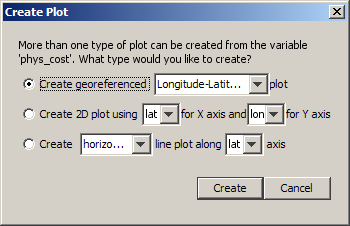
\includegraphics[scale=2.0]{CreatePlot.png}
\end{center}
\caption{\textbf{Panoply} \textsf{Create Plot} dialogue window.}
\label{fig:CreatePlot}
\end{figure}

You can interpolate the data or not (often you may find that it is clearer not to interpolate the data but to leave it as 'blocky' colors corresponding to the resolution of the model), change the scale and colors, overlay continental outline, change the projection, etc etc. Gray cells represent 'dry' grid points, i.e., continental or oceanic crust.
To save plots in \textbf{Panoply} -- from the file menu: \footnotesize\textsf{File}\normalsize, then \footnotesize\textsf{Save Image As ... }\normalsize and then select the location, filename, and graphics format.

%------------------------------------------------

\subsection{Issues with Panoply default settings}

The default settings in \textbf{Panoply}, i.e. those used when a plot is first created, can often mislead. In particular, note:
\begin{itemize}

\vspace{1mm}
\item \footnotesize\textsf{Year }\normalsize (\footnotesize\textsf{Array}\normalsize tab)
        \\ The default is for the very 1st \textit{time-slice} to be displayed rather than the experiment end. The first \textit{time-slice} is numbered from 1 to however many total time-slices have been saved (displayed to the immediate right of the \footnotesize\textsf{Year ,}\normalsize box), and it is this integer number that appears in the \footnotesize\textsf{Year }\normalsize box -- not the year of the data save. Instead, the mid-point year of the time-slice is displayed in a second box (labeled '\footnotesize\textsf{Year mid-point}\normalsize').
        \\ Different \textit{time-slices} to be plotted can be selected by either clicking through the saved year count, or by selecting the save year mid-point from the drop-down list.

\vspace{1mm}
\item \footnotesize\textsf{Scale Range }\normalsize (\footnotesize\textsf{Scale}\normalsize tab)
        \\ The color scale is auto-scaled so that the range always goes from the minimum to maximum displayed value. This can potentially mislead if save years and/or depth/latitude slices are scrolled through as the scale will be automatically adjusted to fit each plot in turn.
        \\ Confusion can also arise for fields with no variation, e.g. atmospheric trace gas concentrations or air temperature -- the auto-scaled plot in these instances has a uniform color but with odd hatching as Panoply dutifully tries to achieve the impossible (creating a scale of multiple colors for a single value).

\vspace{1mm}
\item Zonal averaging (\footnotesize\textsf{Array }\normalsize tab)
        \\ \footnotesize\textsf{Lat-Vert }\normalsize plots are displayed as a zonal mean by default. This is indicated by the tick in the \footnotesize\textsf{Ave }\normalsize box (bottom RH corner). Un-ticking the \footnotesize\textsf{Ave }\normalsize box releases the averaging with the first longitudinal value of the grid now displayed instead. Similar to how Panoply displays years -- the longitudinal grid locations are counter from 1 to typically 36 (depending on the resolution of the ocean grid), with the longitudinal mid-point value in degrees East displayed to the right.
        \\ Different longitudinal sections to be plotted can be selected by either clicking through the grid point number count, or by selecting the longitudinal mid-point from the drop-down list.

\vspace{1mm}
\item Scale bar tick marks (\footnotesize\textsf{Array }\normalsize tab)
        \\ The tick labels on the color scale are displayed by default in the format: \footnotesize\textsf{x.y }\normalsize. If the typical values of the variable are order e.g. 10\begin{math}^{-6}\end{math} you will end up with value labels ranging from \footnotesize\textsf{0.0 }\normalsize to \footnotesize\textsf{0.0 }\normalsize ... This can be most easily resolved in one of two ways:
        \begin{itemize}
\item The format of the label can be changed by selecting a different option from the pull-down \footnotesize\textsf{Tick Label Format }\normalsize box (default == \footnotesize\textsf{\%.1f}\normalsize). For instance, \footnotesize\textsf{\%.2e }\normalsize would give a display in the format \footnotesize\textsf{x.xxEyy }\normalsize (or \footnotesize\textsf{x.xxE-yy}\normalsize) or \footnotesize\textsf{\%.6f }\normalsize would give \footnotesize\textsf{x.xxxxxx}\normalsize.
\item An alternative is to re-scale the values. This is done in the Scaling Factor box in which you set the scale factor in powers of 10. For example: setting \footnotesize\textsf{-6}\normalsize in effect converts units of mol kg\begin{math}^{-6}\end{math} to \begin{math}\mu\end{math}mol kg\begin{math}^{-6}\end{math}.
\end{itemize}

\vspace{1mm}
\item Other things to watch out for include:
\begin{itemize}
\item A plot involving depth, being by default, 'up-side-down'!.
\\This is fixed in the \footnotesize\textsf{Grid}\normalsize tab, and the click button, \footnotesize\textsf{Swap B/T}\normalsize.
\item In \footnotesize\textsf{'Lon-Lat'}\normalsize plots, the modern continental outline being displayed by default.
\\This can be fixed by changing options in the \footnotesize\textsf{Overlay}\normalsize tab.
\end{itemize}

\end{itemize}
\vspace{2mm}

\begin{center}
\textbf{Simply be careful when opening a new plot that you are looking at what you *think* you are looking at (or what you think you are looking at *is* what you are looking at).}
\end{center}

Note that default plotting settings in \textbf{Panoply} can be changed (and saved).

%------------------------------------------------

\subsection{Basic plots -- examples}

\vspace{1mm}
\noindent\rule{4cm}{0.5pt}
\vspace{2mm}

\noindent\textcolor{red}{TO COME ...}

\vspace{1mm}
\noindent\rule{4cm}{0.5pt}
\vspace{2mm}

%------------------------------------------------

\subsection{Difference (anomaly) plots}

It is possible to create an anomaly (difference) maps in \textbf{Panoply} which are essential when analyzing changes in a variable that may be small compared to the global spatial variability. To do this:  

\begin{itemize}
\vspace{1mm}
\item First, open the netCDF results file.
\vspace{1mm}
\item Open the variable of interest, e.g., \texttt{atm\_temp} (surface air temperature) in the 2D netCDF file. 
\vspace{-4mm}
\item From the upper LH corner of the Dataset Browser window, from the drop-down menu, select the name of the plot you have just created (\texttt{atm\_temp} in \footnotesize\textsf{field\_biogem\_2D}\normalsize ...).
\vspace{1mm}
\item From the upper LH corner of the Dataset Browser window, now click on the \footnotesize\textsf{Combine Plot}\normalsize icon.
\\ You now have a plot window that is displaying a difference map. By default, it is showing you the difference between two identical (in time) slices. The two different slices are labeled Array 1 (LH side) and Array 2 (RH side).
\\NOTE: Easier than mucking about with \footnotesize\textsf{Combine Plot}\normalsize, is having open the first dataset, simply drag another variable from the list of variables in the \footnotesize\textsf{Sources }\normalsize window, into the \footnotesize\textsf{Plot }\normalsize window. You can drag either a different, or the same variable, into the \footnotesize\textsf{Plot }\normalsize window.
\end{itemize}
\vspace{2mm}

For instance, you can keep one array (Array 1) fixed to the initial (year 1 (centered on 0.5)) and vary the year in the second array (Array 2). Note that you can select in Panoply whether Array 1 - Array 2 is plotted, or Array 2 - Array 1, or various proportional or relative differences.

If you switch off the auto-scaling feature (\footnotesize\textsf{Always fit to data}\normalsize) you can center the scale so that no change is white, with positive deviations = red and negative = blue by clicking on Center on 0. This is something of a convention in the scientific literature.

The same variable in two different model experiments can also be opened up and analyzed combined: 

\begin{itemize}
\vspace{1mm}
\item Start by opening up both required netCDF files.
\vspace{1mm}
\item Open the variable of interest in one (either one) of the two 2D netCDF data-sets. 
\vspace{1mm}
\item From the upper LH corner of the Dataset Browser window, from the drop-down menu, select the name of the plot you have just created.
\vspace{1mm}
\item Now double-click in the variable in the 2nd netCDF dataset.
\\ You now have a plot window that is displaying a difference map, but of the same variable between two different experiments, rather than two years of the same experiment.
\end{itemize}
\vspace{2mm}

%------------------------------------------------

\subsection{Ocean velocity plots}

By combining the two (horizontal) fields of ocean circulation, rather than a difference plot, \textbf{Panoply} can create a velocity plot. This is a great way of visualizing surface (and deeper) currents and circulation patterns. To do this:

\begin{itemize}
\vspace{1mm}
\item First, open the 3-D netCDF results file.
\vspace{1mm}
\item Open either the \texttt{phys\_u} ('ocean velocity - u') or \texttt{phys\_v} ('ocean velocity - v') field and select a \footnotesize\textsf{Lon-Lat }\normalsize plot.
\vspace{1mm}
\item From the upper LH corner of the \footnotesize\textsf{Sources }\normalsize window, from the drop-down menu, select the name of the plot you have just created.
\vspace{1mm}
\item Now double-click on the other velocity variable (whichever of the u and v fields you did not open first).
\vspace{1mm}
\item By default you get a difference map, which is pretty useless really. From the drop-down \footnotesize\textsf{Plot }\normalsize menu box (which should be displaying 'Array 1 - Array 2' by default) select: \footnotesize\textsf{Vector Magnitude }\normalsize(bottom of the list).
\\ You now have a plot window that is displaying the ocean velocity field, with arrows indicating the direction and speed (length of the arrow) together with an interpolated color background of the speed.
\end{itemize}
\vspace{2mm}

You can re-scale the velocity arrows to more clearly display the circulation pattern by altering the \footnotesize\textsf{Scale Length }\normalsize value (\footnotesize\textsf{Contours \& Vectors }\normalsize tab). A value of 0.1 is a reasonable choice for surface currents. e.g. see Figure \ref{fig:cgenie_currents}.

If you want to display deeper (in the ocean) current fields and/or different time-slices, take care that the depth level (/time-slice) in both LH and RH sides of the \footnotesize\textsf{Array(s) }\normalsize panel must be changed to the same value. If displaying deeper current fields, then the velocity vectors will have to be further re-scaled (to a smaller value) in line with the lower velocities at depth compared to the surface.

\newpage

\begin{figure}[ht]
\begin{center}
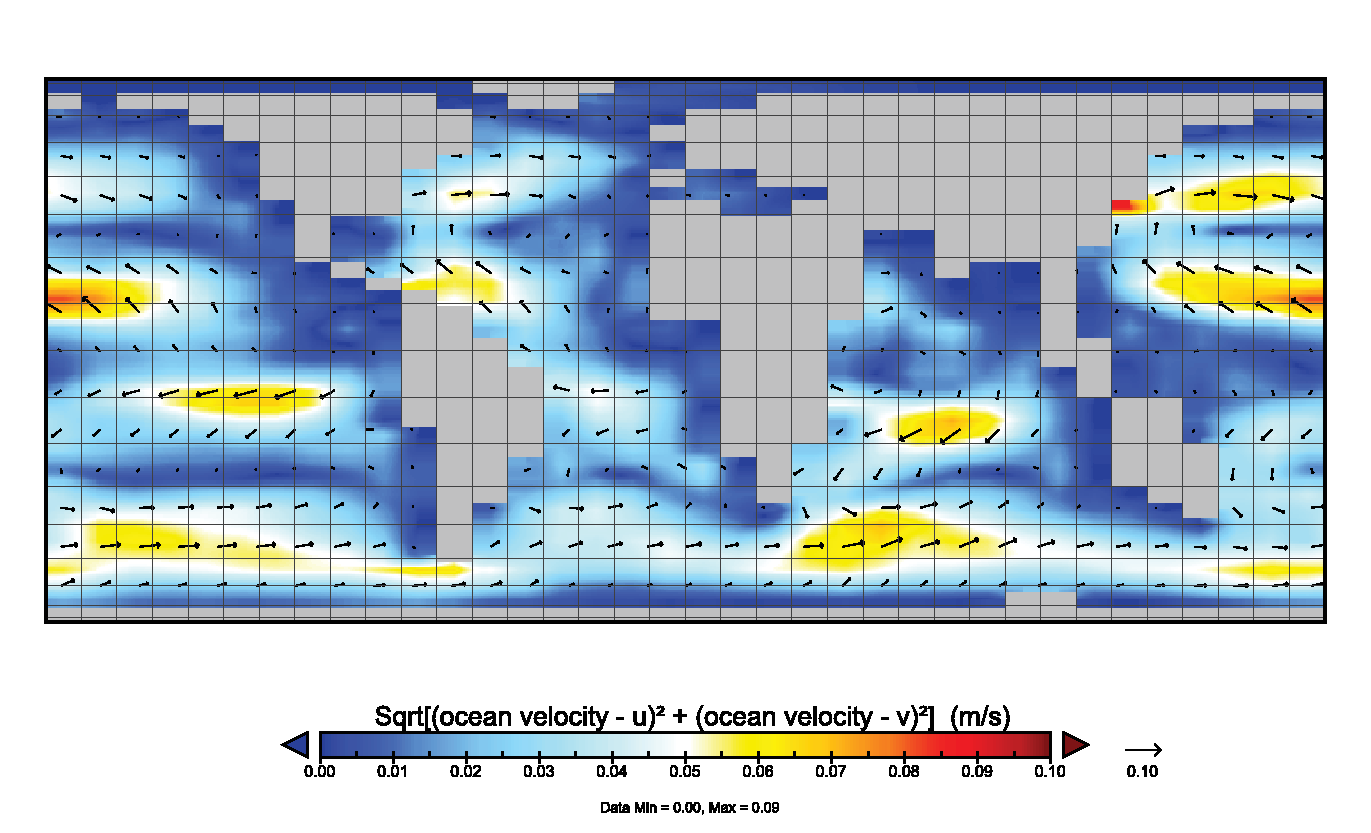
\includegraphics[scale=0.5]{cgenie_currents.eps}
\end{center}
\caption{Example (modern) ocean surface velocity (current) map.}
\label{fig:cgenie_currents}
\end{figure}

%------------------------------------------------

\newpage

%------------------------------------------------

\section{MATLAB plotting}

%------------------------------------------------

\subsection{MATLAB 101}

If you need a tutorial on \textbf{MATLAB}, either as a refresher, or because you have not used the program before, refer to (and/or work through) the following sections of the \href{https://github.com/derpycode/matlabananas\#matlabananas}{matlabananas} \textbf{MATLAB} textbook:

\vspace{2pt}
\begin{itemize}
\vspace{1pt}
\item Chapter 1 --  this covers the very basics of using \textbf{MATLAB}, what variables are, including scalars (e.g. single numbers), vectors (1D array), matrices (2D array) and higher order arrays, now to index and carry out basic manipulation of arrays, basic data loading and saving and plotting.
\vspace{1pt}
\item Sections 2.1 and 2.2 of Chapter 2, which cover creating (script) programs -- i.e. adding all your \textbf{MATLAB} commands to a file (a \footnotesize\textsf{.m }\normalsize or '\footnotesize\textsf{m-file }\normalsize') and running the file, and \textit{functions} -- programs (\footnotesize\textsf{m-file}\normalsize s) where one or more parameters might be passed into the \textit{function} when it is called (e.g. at the command line), and potentially variables returned.
\vspace{1pt}
\item In Chapter 3 -- subsection 3.1.3 deals with reading in netCDF format data, which is the \textbf{muffin} format for spatial data. Section 3.2 deals with more advanced 2D plotting (also of direct relevance to \textbf{muffin} data processing and visualization using \textbf{MATLAB}).
\end{itemize}
\vspace{2pt}

%------------------------------------------------

\subsection{MATLAB and ASCII (\textit{time-series})}

The \textit{time-series} (\textsf{\footnotesize .res}) output of \textbf{BIOGEM} are in a simple plain text (ASCII) format. These can be read in very easily in \textbf{MATLAB} using the \texttt{load} command. Note that a brief description of each column of data in the \textit{time-series} files appears on the first first line of the file, and that prefixing this is a \texttt{\%} symbol, that \textbf{MATLAB} ignores. Hence only the columns of data gets read in by default using \texttt{load} :) \footnote{There are also other \textbf{MATLAB} commands for reading in text data -- refer to to the \href{http://www.seao2.info//teaching/201718.GEO111/GEO111.pdf}{\textbf{MATLAB} programming text}.} For example:

\small\begin{verbatim}
>> co2=load('biogem_series_atm_pCO_2.res','-ascii');
>> plot(co2(:,1),1.0E6*co2(:,3));
\end{verbatim}\normalsize

\noindent loads in the atmospheric \(CO_{2}\) time-series file (assigning it to the array variable \texttt{co2}), and then plots (as a line graph) the 3rd column (\(CO_{2}\) concentration) vs. the first (time). Because concentrations are saved in units of atmospheres, a factor of \texttt{1.0E6} is applied to concert to \(\mu atm\). Equivalently:

\small\begin{verbatim}
>> co2=load('biogem_series_atm_pCO2\).res','-ascii');
>> scatter(co2(:,1),1.0E6*co2(:,3));
\end{verbatim}\normalsize

%------------------------------------------------

\subsection{MATLAB 'Import Data' ...}

You can also import the time-series files by clicking on the \footnotesize\textsf{Import Data }\normalsize icon:

\begin{itemize}
\vspace{1pt}
\item Navigate to the \textbf{BIOGEM} sub-directory of your experiment results directory. Ensure that \footnotesize\textsf{All Files }\normalsize is selected and click on the time-series file you want.
\vspace{1pt}
\item \textbf{MATLAB} ignores the header lines, and it should be safe to simply click on \footnotesize\textsf{Import Selecftion }\normalsize for all columns, or select what you want to plot -- typically year (the first column) and another one.
\vspace{1pt}
\item A default variable name -- the filename minus the underscore characters -- will appear listed in the \textbf{MATLAB} \footnotesize\textsf{Workspace window }\normalsize. Double-click on the variable name to open up the imported data in a table view. If you select columns to plot, and then head over to the main \footnotesize\textsf{PLOTS }\normalsize tab, a range of plotting options are provided and a plot can be generated by clicking on one of the plotting icons.\footnote{Note that if you have not selected any data columns, then all the plotting icons are disabled and greyed out in the \footnotesize\textsf{PLOTS }\normalsize tab.}
\vspace{1pt}
\item Labels can be added, scales and markers changed, etc etc, in the \footnotesize\textsf{Figure window }\normalsize.
\end{itemize}
\vspace{2pt}

Note that as the data has been imported as an array in \textbf{MATLAB}, you can also plot directly from the command line. (And indeed, you could also have loaded the data from the command line.)

%------------------------------------------------

\subsection{MATLAB and netCDF (\textit{time-slice})}

\noindent Basically -- the only hard part, having opened the \textit{netCDF} file is in correctly deducing which dimension in an extracted data array is   longitude, latitude, (sometimes depth), or time. Mostly this should be pretty obvious from inspecting the \textbf{MATLAB} \footnotesize\textsf{Workspace }\normalsize window (assuming you have a column for \footnotesize\textsf{Size }\normalsize selected to be displayed), or using the \texttt{size} command.\footnote{It also turns out that the order of dimensions for a variable read in by \textbf{MATLAB}, is the opposite of the order listed in the \textsf{Variable} window of \textbf{Panoply}.} Once you have done this, you can plot slices, scale data, average or otherwise process data, extract locations at specific locations, etc etc.

As an example -- in \textbf{MATLAB}, first either change directory to the \textsf{\small biogem} directory of a set of \textbf{muffin} results, or from where-ever you are, add a path to the location of the \textsf{\small biogem} directory. To open the 2D \textbf{BIOGEM} netCDF results file, type:
\begin{verbatim}
>> ncid = netcdf.open('fields_biogem_2d.nc','nowrite');
\end{verbatim}

To extract a variable, you first need to find its ID from its name:
\begin{verbatim}
>> varid = netcdf.inqVarID(ncid,NAME);
\end{verbatim}
where \texttt{NAME} is a place-holder for the name of he variable (as a string). You might need to use \textbf{Panoply} to display all the different variable names. Or, you can list all the variables and stuff in the netCDF file using \texttt{ncdisp}:
\begin{verbatim}
>> ncdisp('fields_biogem_2d.nc') 
\end{verbatim}

Having, by one means or another, identified the name of the variable you are interested in, you can recover its ID and then the data itself, for example, for \textsf{\footnotesize atm\_temp} (\textsf{\footnotesize surface air temperature}):
\begin{verbatim}
>> varid = netcdf.inqVarID(ncid,'atm_temp');
>> data  = netcdf.getVar(ncid,varid);
\end{verbatim}

In loading in the variable, you end up with a multi-dimensional array -- 2 spatial dimensions and if you have more than 1 \textit{time-slice} of data saved, 1 temporal dimension (and if you loaded in the \textbf{BIOGEM} 3D netCDF file, you end up with a 4-dimensional array). \textbf{MATLAB} reports the size of the array in the \textsf{\footnotesize Workspace window} (depending on which column display options you have selected). In the example here, which took the experiment \textsf{\footnotesize EXAMPLE.worjh2.Caoetal2009.RCP6p0}, the array for atmospheric temperature is reported as \(36\times36\times8\).\footnote{Although note that in \textbf{Panoply}, it is reported as \textsf{\scriptsize atm\_temp(time=8, lat=36, lon=36)}.} so the last of the 8 time-slices would  be accessed as:
\begin{verbatim}
>> data_last = data(:,:,8);
\end{verbatim}
or
\begin{verbatim}
>> data_last = data(:,:,end);
\end{verbatim}

Panoply reports variables in the the \textbf{BIOGEM} 3D netCDF file as having dimensions of: (\textit{time, zt, lat, lon}) (e.g. (time=13, zt=16, lat=36, lon=36)) whereas \textbf{MATLAB} reads it in the reverse order. For instance, if we load in the (3D) ocean temperature field:
\begin{verbatim}
>> ncid = netcdf.open('fields_biogem_3d.nc','nowrite')
>> varid = netcdf.inqVarID(ncid,'ocn_temp');
>> data  = netcdf.getVar(ncid,varid);
\end{verbatim}
and then type:
\begin{verbatim}
>> size(data)
ans =
    36    36    16    13
\end{verbatim}
we get an array orientated as (\textit{lon, lat, zt, time}).\footnote{\textit{zt} is the depth level in the ocean.} The final time-slice would hence then be accessed:
\begin{verbatim}
>> data_last = data(:,:,:,end);
\end{verbatim}
with \texttt{data\_last} now becoming a 3D array with dimensions (\textit{lon, lat, zt}).

\vspace{2mm}
There are three key things to remember at this point:

\begin{enumerate}
\setlength{\itemindent}{.2in}

\vspace{1mm}
\item Firstly, the depth levels are read such that index \texttt{1} is the surface, and \texttt{16} is the deepest ocean depth level (in this case, otherwise it is \texttt{8}).

\vspace{1mm}
\item For the lon-lat part -- (\textit{lon, lat}) equates to \textit{row}\textit{}s vs. \textit{columns} in \textbf{MATLAB}, and hence if you were to plot e.g. the surface ocean slice:
\begin{verbatim}
>> imagesc(data_last(:,:,1));
\end{verbatim}
you will end up with the plot on its side, with latitude along the \textit{x}-axis and longitude on the \textit{y}-axis.
\\You can exchange rows and columns in \textbf{MATLAB} with the \textit{transpose operator} (see programming/\textbf{MATLAB} book):
\begin{verbatim}
>> imagesc(data_last(:,:,1)');
\end{verbatim}
but ... this still leaves you with an up-side-down plot, because \textbf{MATLAB} reads from the first row down, whereas in latitude, you are expecting to read from -90 degrees up (towards the N pole). \texttt{flipud} accomplishes the final transformation:
\begin{verbatim}
>> imagesc(flipud(data_last(:,:,1)'));
\end{verbatim}

\vspace{1mm}
\item The final complication is that \textbf{muffin} netCDF output uses a special value to represent an invalid or null number, e.g. for ocean temperature where the grid point is land (and an ocean temperature value would have no meaning). In the netCDF definition, \textbf{Panoply} is told what the special number is, hence it shows land in grey when plotting ocean variables.

Panoply reports this as: \textsf{\footnotesize missing\_value = 9.969209968386869E36}.

\vspace{1mm}
There is no easy way (that I can see!) to get \textbf{MATLAB} to deal with this for you, so you need to search and replace this value, e.g.:
\small\begin{verbatim}
>> null=9.969209968386869E36;
>> data_last(find(data_last==null))=NaN;
\end{verbatim}\normalsize
which searches for this null value and replaces it with a \texttt{NaN} (so that now it can be simply plotted).

\end{enumerate}
\vspace{2mm}

Once you are done accessing data, it is good practice to close the netCDF file after you are done with it:
\begin{verbatim}
>> netcdf.close(ncid);
\end{verbatim}

The question then remains: what do you actually 'do' with it in \textbf{MATLAB}?

%------------------------------------------------

\subsubsection{Plotting sections}

For a quick look-see, \texttt{imagesc} (as per above) is handy.

\noindent For more advanced plotting (and for presentation) -- refer to the \textbf{matlabananas} \textbf{MATLAB} programming text.

\noindent As per above, horizontal (lon-lat) fields can be extracted from 2D \textit{netCDF} output by: \texttt{data(:,:,time)} and from 3D by: \texttt{data(:,:,zt,time)}. Obviously, you could also extract lon-depth via: \texttt{data(:,lat,:,time)} and lat-depth via: \texttt{data(lon,:,:,time)}.

\noindent Anomalies (with time) are created: \texttt{data(:,:,:,time2)-data(:,:,:,time2)}.

Typically, except a little trial-and-error in extracting the dimensions you want, and also in correcting the orientation of the matrix or resulting plot.

%------------------------------------------------

\subsubsection{Calculating inventories}

Often, the inventory (total mass or number of moles) of the ocean or atmosphere is useful to know, particularly as a function of time. For the ocean (or atmosphere) as a whole, the \textit{time-series} output files report this (alongside the mean global concentration).

You can also calculate this with \textbf{MATLAB} from the netCDF output. Fields of ocean concentration are saved in the 3D output (and atmospheric concentrations in the 2D output). To convert concentration in the ocean, in units of \(molkg^{-1}\) you'll need to know the mass of each ocean cell, in units of \(kg\). 

When saving using save option \texttt{9}, or \texttt{99}\footnote{Parameter \texttt{bg\_par\_data\_save\_level} -- see earlier.}, you save the 'physics' of the ocean model, which is actually mostly just the grid information, such as cell area, thickness, latitude and longitude edges and midpoints, depth edges and mid point. Also saved are the masses and volumes of the grid of cells. So to derive an array of cell tracer inventories from an array of concentrations, and the array of cell masses (variable \textsf{\footnotesize phys\_ocn\_M}), you'd write:

\pagebreak 

\small\begin{verbatim}
varid = netcdf.inqVarID(ncid,'ocn_temp');
data  = netcdf.getVar(ncid,varid);
varid = netcdf.inqVarID(ncid,'phys_ocn_M');
mass  = netcdf.getVar(ncid,varid);
inventory = data(:,:,:,time).*mass(:,:,:,time);
\end{verbatim}\normalsize
\noindent Before summing \texttt{inventory} to determine the global total inventory, you will, as before, have to deal with the null values (converting them to \texttt{NaN}) and then deal with the presence of \texttt{NaN}s in the array when summing ...

The advantage of doing the calculations in \textbf{MATLAB} (despite being provided with the global mean and inventory in the time-series files) is that you could calculate the inventory of a tracer (/substance) for just the ocean surface, or just a specific region of band of latitude. Or you could calculate the mean concentration for just a specific region of the ocean.\footnote{In calculating mean concentrations, you'll need to volume or mass weight the concentrations, and hence still need to use one of the physics variables.}

%----------------------------------------------------------------------------------------
%       CHAPTER X
%----------------------------------------------------------------------------------------

\cleardoublepage

\chapterimage{chx-plotting.png} % Chapter heading image

\chapter{muffinplot}

\hfill \break

\vspace{24mm}

\noindent The \textbf{muffinplot} suite of \textbf{MATLAB} functions provides a means of plotting a variety of output reproducibly (by means of  saved parameter file) and with the potential for automation (i.e. automatically generating the same analysis for a large number of different experiments).

The functions comprising this software suite include:

\begin{itemize}[noitemsep]
\vspace{1mm}
\item \footnotesize\textsf{plot\_fields\_biogem\_2d}\normalsize -- lon-lat plots from the 2D \textbf{biogem} output.
\vspace{1mm}
\item \footnotesize\textsf{plot\_fields\_biogem\_3d\_i}\normalsize -- lat-depth plots from the 3D \textbf{biogem} output. 
\vspace{1mm}
\item \footnotesize\textsf{plot\_fields\_biogem\_3d\_k}\normalsize -- lon-lat plots from the 3D \textbf{biogem} output.
\vspace{1mm}
\item \footnotesize\textsf{plot\_fields\_ccd}\normalsize -- analsysis of the 'CCD' (from both \textbf{biogem} 2D and \textbf{sedgem} 2D output).
\vspace{1mm}
\item \footnotesize\textsf{plot\_fields\_sedgem\_2d}\normalsize -- lon-lat plots from the 2D \textbf{sedgem} output.
\vspace{1mm}
\item \footnotesize\textsf{plot\_histc\_2d}\normalsize -- a generic color-coded histogram function.
\vspace{1mm}
\item \footnotesize\textsf{plot\_sedcore}\normalsize -- down-core plots from \textbf{sedgem} sedcore output.
\vspace{1mm}
\item \footnotesize\textsf{plot\_timeseries\_biogem}\normalsize -- time-series plots from \textbf{biogem} time-series output.
\end{itemize}
Note that at this current time, there is no facility for lon-depth plotting.

Most of the plots also perform additional functions (which can be generally disabled if not wanted), such as plotting and saving zonal or depth profiles, plotting difference maps, plotting and labelling data on maps and carrying out model-data fit statistics and plotting, extracting model values at data locations.

The following sections provide an overview and examples of such plotting and analysis.

%------------------------------------------------

\section{Installation}

\textbf{muffinplot} can be obtained from \href{https://github.com/derpycode/muffinplot\#https://github.com/derpycode/muffinplot}{github}. If you do not have a \textbf{git} client on your computer (and hence can clone the repository locally), then simply download an archive of the code (from \footnotesize\textsf{\textcolor[rgb]{0,0.501961,0}{clone or download }}\normalsize -- pick \textsf{\footnotesize Download ZIP}).

When you unpack (or clone) \textbf{muffinplot}, you should see 3 directories -- \footnotesize\textsf{EXAMPLES}\normalsize, and \footnotesize\textsf{MASKS}\normalsize,\ \footnotesize\textsf{source}\normalsize, a series of \footnotesize\textsf{.m }\normalsize files, and a single lonely \footnotesize\textsf{.ps }\normalsize graphics file (\footnotesize\textsf{colorscales.ps}\normalsize). The \footnotesize\textsf{.m }\normalsize files are split into filenames with or without the label \footnotesize\textsf{SETTINGS }\normalsize -- the ones without are code files (\textit{functions}), and the ones with the word \footnotesize\textsf{SETTINGS }\normalsize in their filename, contain parameter settings for plotting.

By default (the parameters can be changed if you wish), wherever you run the \textbf{muffinplot} plotting function from, requires that you have a subdirectory called \footnotesize\textsf{cgenie\_output}\normalsize, where you will place the (complete) \textbf{muffin} experiment output directories (i.e. the contents of \footnotesize\textsf{cgenie\_output }\normalsize should look like the contents of \footnotesize\textsf{cgenie\_output }\normalsize on your cluster account\footnote{Although you do not need to copy \uline{all} the results over ... just the experiments that you wish to plot up.}). If you do any model-data analysis, by default, a directory \footnotesize\textsf{DATA }\normalsize is also expected. Mask files reside in the \footnotesize\textsf{MASKS}\normalsize\ subdirectory of the \textbf{muffinplot} installation, or in your current directory, or anywhere in the \textbf{MATLAB} path.

The simplest option might be to unpack/clone \textbf{muffinplot} to a directory containing \footnotesize\textsf{cgenie\_output }\normalsize and hence all your experimental results directories.\footnote{However, the \textbf{muffinplot} functions do not have to be run from the same directory that you are in -- you can install them somewhere convenient, and then with \textbf{MATLAB} set to a directory containing a \textsf{cgenie\_output} experiment results directory, you can:
\\\texttt{>> addpath(PATH)}
\\where \texttt{PATH} is the path to the directory where \textbf{muffinplot} is installed.}
In other words:
\begin{enumerate}[noitemsep]
\vspace{1mm}
\item Create some local directory e.g. called \footnotesize\textsf{RESULTS}\normalsize.
\vspace{1mm}
\item Create a subdirectory in \footnotesize\textsf{RESULTS }\normalsize called \footnotesize\textsf{cgenie\_output}\normalsize.
\vspace{1mm}
\item Drag your experiment results folders across into the subdirectory \footnotesize\textsf{cgenie\_output}\normalsize, as per the directory structure on the cluster. (Or drag the archived files and unpack them.)
\vspace{1mm}
\item Install \textbf{muffinplot} in the \footnotesize\textsf{RESULTS }\normalsize directory.
\vspace{1mm}
\item Change the \textbf{MATLAB} working directory to \footnotesize\textsf{RESULTS}\normalsize.
\end{enumerate}
\vspace{2mm}

The plotting functions are run simply by typing their name and passing a list of parameters (comma-separated, with the complete list enclosed in parentheses). By default,   the \footnotesize\textsf{SETTINGS }\normalsize files need to be in the same directory as you are running the \textit{functions} from, or in one of the \textbf{MATLAB} paths. Results are saved to a subdirectory that by default is called \footnotesize\textsf{PLOTS}\normalsize, which will be created for you if it does not already exist.

All the plotting functions provide some manner of 'help', that can be obtained by typing at the command line:
\vspace{-2pt}\begin{verbatim}
>> help FUNCTIONNAME
\end{verbatim}\vspace{-2pt}
where \texttt{FUNCTIONNAME} is the function name (as per listed above).

%------------------------------------------------

\section{Time-series plotting}

The \textbf{muffinplot} function \textsf{\footnotesize plot\_timeseries\_biogem.m} provides a facility to plot \textbf{BIOGEM} \textit{time-series} (\textsf{\small .res}) output.\footnote{Obviously -- there are lots of different and easy ways of plotting plain text output in the form of a simple column format.} You can use \textbf{MATLAB} \texttt{help} on the function name to detail the parameters that need to be passed (and examples).

The \textsf{\footnotesize plot\_timeseries\_biogem} plotting function plots a basic set of time-series variables by default. It then, enables a set up up to 3 additional variables to be plotted. It is also associated with a file of parameter values (\textsf{\footnotesize plot\_timeseries\_SETTINGS.m} by default) for fine-tuning plots.

The plotting function requires a list of parameters to be passed in the argument list, i.e.:
\begin{verbatim}
>> plot_timeseries_biogem(PAR1,PAR2,PAR3, ... PARn)
\end{verbatim}

These are, in order:

\vspace{1mm}
\begin{enumerate}
\item \texttt{PEXP1} -- \textit{string} \(\rightarrow\) the (first) experiment name.
\item \texttt{PEXP2} -- \textit{string} \(\rightarrow\)  is the name of the 2nd (optional) experiment. If no second experiment is selected, then a null string value must be passed, i.e., \texttt{''}.
\item \texttt{PTMIN} -- \textit{real} \(\rightarrow\) minimum plotted time (\textit{x}-axis).
\item \texttt{PTMAX} -- \textit{real} \(\rightarrow\) maximum plotted time (\textit{x}-axis).
\item \texttt{PDATA1} -- \textit{string} \(\rightarrow\) time-series variable name for additional data to plot.
\\Omit the '\texttt{biogem\_series\_}' and '\texttt{.res}' parts of the filename.
\\Leave blank, i.e., '', for no additional data panel.
\item \texttt{PDATA1N} -- \textit{integer} \(\rightarrow\) the column number of the data in the time-series file.
\item \texttt{PDATA2} -- \textit{string} \(\rightarrow\) time-series variable name for additional data to plot.
\item \texttt{PDATA2N} -- \textit{integer} \(\rightarrow\) the column number of the data in the time-series file.
\item \texttt{PDATA3} -- \textit{string} \(\rightarrow\) time-series variable name for additional data to plot.
\item \texttt{PDATA3N} -- \textit{integer} \(\rightarrow\) the column number of the data in the time-series file.
\item \texttt{POPT} -- \textit{string}\(\rightarrow\) The string for an alternative plotting parameter set.
\\If an empty\texttt{ ('') }value is passed as this parameter, then the default parameter set file is used.
\item \texttt{PNAME}  -- \textit{string}\(\rightarrow\) The string for an alternative filename.
\end{enumerate}
\vspace{2mm}
Note that if an empty value is passed as this parameter, then a filename is automatically generated.

A simple example usage would be:

\begin{verbatim}
>> plot_timeseries_biogem('myexperiment','',0.0,10000.0,'',0,'',0,'',0,'','')
\end{verbatim}
where \texttt{myexperiment} is the name of the 1st experiment, followed by and empty string (\texttt{''}) indicating no second experiment. The results are to be plotted from 0.0 to 10000.0 years (the 2 following parameters; \texttt{0.0,10000.0}). Then, no additional (maximum 3) optional parameters are requested, and hence the next parameters passed are: \texttt{'',0,'',0,'',0}. Finally, the default plotting parameter set is required, and no specific alternative filename is ot be used, accounting for the final 2 empty strings passed.

By default, \textsf{\footnotesize plot\_timeseries\_biogem} plots 2 panels of data, both with 2 (LH\ and RH) axes:

\begin{enumerate}[noitemsep]
\vspace{1mm}
\item Atmospheric \(CO_{2}\). Note that if the experiment was not \(CO_{2}\)-enabled (i.e. not run with a global carbon cycle), a warning is given and 'fake' data (actually, random numbers) is plotted.
\vspace{1mm}
\item Atmospheric \(\delta ^{13}CO_{2}\). Note that if the experiment was not \(\delta ^{13}CO_{2}\)-enabled (i.e. not run with a global carbon cycle), a warning is given and 'fake' data is plotted.
\vspace{1mm}
\item Atmospheric temperature (as a global mean, annual average).
\vspace{1mm}
\item Fractional (percentage) sea-ice extent.
\end{enumerate}
\vspace{2mm}

Additional model outputs can then be added by listing them in the function call. For example, to also plot the global overturning strength, which is contained in the file \footnotesize\textsf{biogem\_series\_misc\_opsi.res}\normalsize, you would add \texttt{'misc\_opsi',3}\footnote{Don't forget that you omit the '\texttt{biogem\_series\_}' and '\texttt{.res}' parts of the filename.}, where the \texttt{3} indicates the 3rd column of data in the file is to be plotted, which in this case is the global maximum overturning value (and the 2nd column is the minimum value). The complete line looks like:
\small\begin{verbatim}
>> plot_timeseries_biogem('myexperiment','',0.0,10000.0,'misc_opsi',3,'',0,'',0,'','')
\end{verbatim}\normalsize

By default, the plotted variables are all auto-scaled. To specify the y-axes, you will need to edit the plotting settings parameter file: \footnotesize\textsf{plot\_timeseries\_SETTINGS.m}\normalsize. For the default plotted 4 results variables, the minimum and maximum y-axis limits are specified in the section:
\vspace{1mm}
\begin{itemize}
\item[] \texttt{axis\_pCO2min = 0.0;}
\item[] \texttt{axis\_pCO2max = 0.0;}
\item[] \texttt{axis\_d13Cmin = 0.0;}
\item[] \texttt{axis\_d13Cmin = 0.0;}
\item[] \texttt{axis\_Tatmmin = 0.0;}
\item[] \texttt{axis\_Tatmmin = 0.0;}
\item[] \texttt{axis\_icemin = 0.0;}
\item[] \texttt{axis\_icemin = 0.0;}
\end{itemize}
\vspace{2mm}
The default zero values here, tell the plotting function to create an auto-scale for the y-axis.\footnote{Note the units of atmospheric \(CO_{2}\) as \(\mu atm\).} Following this in the parameter file, are the settings for the optional variable plotting:
\vspace{1mm}
\begin{itemize}
\item[] \texttt{axis\_data1\_min = 0.0;}
\item[] \texttt{axis\_data1\_max = 0.0;}
\item[] \texttt{axis\_data2\_min = 0.0;}
\item[] \texttt{axis\_data2\_max = 0.0;}
\item[] \texttt{axis\_data2\_min = 0.0;}
\item[] \texttt{axis\_data2\_max = 0.0;}
\end{itemize}
\vspace{2mm}

Note that if you want instead to copy and rename and then edit this settings file, you will need to pass the new (non-default) filename when calling the plotting function. For example, if you created a new parameter settings file: \footnotesize\textsf{settings\_NEW.m }\normalsize, then the \textit{function} call would look like:
\small\begin{verbatim}
>> plot_timeseries_biogem('myexperiment','',0.0,10000.0,'',0,'',0,'',0,'settings_NEW','')
\end{verbatim}\normalsize

%------------------------------------------------

\section{Spatial plotting}

%------------------------------------------------

\subsubsection{Overview}

4 of the \textbf{muffinplot} plotting functions provide spatial (2D) plotting capabilities:
\vspace{2mm}
\begin{itemize}

\item \texttt{plot\_fields\_biogem\_2d}
\\Plot a 2-D field from: \footnotesize\textsf{fields\_biogem\_2d.nc}\normalsize.

\item \texttt{plot\_fields\_biogem\_3d\_i}
\\Plot a vertical-meridional (2-D) slice through the ocean (i.e., all cells have the same \texttt{i} (longitudinal) coordinate value) from: \footnotesize\textsf{fields\_biogem\_3d.nc}\normalsize.
\\Options are  provided for averaging longitudinally over a supplied mask, which may be the entire ocean and hence giving a global meridional cross-sectional mean, of a specific ocean basin, or may be a single cell 'wide' longitudinally and take a meandering path hence simulating an ocean transect. An option is also provided to overlay an ocean circulation stream-function.

\item \texttt{plot\_fields\_biogem\_3d\_k.m}
\\Plot a horizontal slice through the ocean from: \footnotesize\textsf{fields\_biogem\_3d.nc}\normalsize.
\\An option is provided for overlaying ocean circulation (velocity fields). Water column integrals  can also be calculated and displayed, as well as benthic surfaces, and the function can also determine the spatial distribution of the maximum or minimum value occurring anywhere in the water column (or portion of the water column).

\item \texttt{plot\_fields\_sedgem\_2d}
\\Plot a 2-D field from: \texttt{fields\_sedgem\_2d.nc}.

\end{itemize}
\vspace{2mm}

All 4 plotting functions can also overlay observed data and create difference (anomaly) maps -- either between different experiments, time-slices, or variables, or between model and data and provide summary statistics regarding the difference.

\subsubsection{Argument (parameter) list}

All 4 plotting functions share exactly the same format of parameters\footnote{Parameters can be in for form of strings, in which case they must be given as a series of characters enclosed in inverted commas \texttt{''}; as real numbers, e.g. \texttt{999.5} or \texttt{9.995E2}; or integers, e.g. \texttt{2}, \texttt{10}.} passed in the argument list:

\vspace{-2mm}
\small\begin{verbatim}
>> FUNCTIONNAME(PAR1,PAR2,PAR3, ... PARn)
\end{verbatim}\normalsize
\vspace{-2mm}
\noindent i.e. take a (long!) list of parameters. These are (in order):

\vspace{1mm}
\noindent Firstly, a series of parameters for defining experiment, variable, and year:

\vspace{1mm}
\begin{enumerate}
\item \texttt{PEXP1} -- \textit{string} -- is the name of the 1st (main) experiment. A results directory with the same name must exist in the directory \footnotesize\textsf{cgenie\_output}\normalsize\footnote{Or alternative directory if the default file path settings have been changed.}. 
\item \texttt{PEXP2} -- \textit{string} -- is the name of the 2nd (optional) experiment. If no second experiment is selected, then a null string value must be passed, i.e., \texttt{''}.
\item \texttt{PVAR1} -- \textit{string} -- is the name of the 1st (main) variable. If no valid variable value is given, a list of valid variable names will be printed out.\footnote{As a string, the value must be encased in inverted commas: \texttt{''}.}
\item \texttt{PVAR2} -- \textit{string} -- is the name of the 2nd (optional) variable. If no second variable is selected, then a null string value must be passed, i.e., \texttt{''}.
\item \texttt{PT1} -- \textit{real} (or \textit{integer}) -- is the value of the 1st (main) time-slice. If no valid variable value is given, a list of valid variable names will be printed out.\footnote{As \textbf{sedgem} does not save multiple and/or time-specific data, a dummy value (anything) is entered here.}
\item \texttt{PT2} -- \textit{real} (or \textit{integer}) -- is the value of the 2nd (optional) time-slice. If no second time-slice is selected, then enter \texttt{-1}.\footnote{As \textbf{sedgem} does not save multiple and/or time-specific data, a dummy value (anything) is entered here.}
\end{enumerate}
\vspace{1mm}

Then there are 2 parameters for plotting sub-sets of the 2D or 3D data (essential for 3D data which cannot be usefully visualized in raw form):

\vspace{1mm}
\begin{enumerate}
\item \texttt{PIK} -- \textit{integer} -- varies in its interpretation and is discussed below.
\item \texttt{PMASK} -- \textit{string} -- is the name of an optional (2D) mask. A null string (\texttt{''}) must be passed if no mask is requested. A file with the same name (plus an extension \footnotesize\textsf{.dat}\normalsize) must exist in the directory \footnotesize\textsf{MASKS}\normalsize\footnote{Or alternative directory if the default file path settings have been changed.}. The interpretation of this parameter differs slightly between functions (below).
\end{enumerate}
\vspace{1mm}

Next come options for plotting scale control:

\vspace{1mm}
\begin{enumerate}
\item \texttt{PCSCALE} -- \textit{real} (or \textit{integer}) -- is the scale factor for the plot. For example, to plot in micro molar (umol kg-1) units, enter; \texttt{1e-6}. The plot is auto-scaled if a value of zero (\texttt{0.0}) is entered.
\item \texttt{PCMIN} -- \textit{real} (or \textit{integer}) -- is the minimum scale value.
\item \texttt{PCMAX} -- \textit{real} (or \textit{integer}) -- is the maximum scale value.
\item \texttt{PCN} -- \textit{integer} -- is the number of (contour) intervals between minimum and maximum scale values.
\end{enumerate}
\vspace{1mm}

Finally, there are 3 parameters for: specifying discrete (observed) data to be plotted (and analyzed against model projections), for specifying the plotting parameter file to be used, and for substituting an alternative filename for all the output:

\vspace{1mm}
\begin{enumerate}
\item \texttt{PDATA} -- \textit{string} -- is the filename containing the an overlay data set, which must be formatted as separated columns. The precise number and type of columns varies between different functions and also the plotting options chosen, and are hence discussed later. The full filename of this file must be give, \uline{including} any extensions (e.g. \footnotesize\textsf{.dat }\normalsize, \footnotesize\textsf{.txt}\normalsize). This parameter must be passed as a \textit{string}; leave blank, i.e., \texttt{''}, for no overlay data.
\item \texttt{POPT} -- \textit{string} -- is the \footnotesize\textsf{m-file }\normalsize filename (excluding the \footnotesize\textsf{.m }\normalsize extension) containing the plotting options (\footnotesize\textsf{SETTINGS}\normalsize). This parameter must be passed as a string; leave blank, i.e., \texttt{''}, in order to load the default file (\footnotesize\textsf{plot\_fields\_SETTINGS}\normalsize).
\item \texttt{PNAME} -- \textit{string} -- is the string for an alternative series of output filenames. This parameter must be passed as a string, e.g., \texttt{'experiment2'}. If an empty (i.e., \texttt{''}) value is passed to this parameter then the output filenames will be automatically generated.
\end{enumerate}
\vspace{1mm}

\vspace{1mm}
The basic parameter list for all 4 plotting functions\footnote{Note that for \texttt{plot\_fields\_sedgem\_2d} several of the parameters are redundant but \uline{must} still be included (typically as zeros). This is in order to retain a common parameter list format between all the different plotting functions.} is hence:
\footnotesize
\vspace{-4pt}\begin{verbatim}
>> FUNCTIONNAME(PEXP1,PEXP2,PVAR1,PVAR2,PT1,PT2,PIK,PMASK,PCSCALE,PCMIN,PCMAX,PCN,PDATA,POPT,PNAME);
\end{verbatim}\vspace{-4pt}
\normalsize

\subsubsection{Function specific interpretation of PIK and PMASK}

A note on the different behaviour of 2 of the passed parameters, depending on whcih plotting function is used -- \texttt{PIK}, and to some extent, \texttt{PMASK}, have quite different interpretations depending on the particular plotting function used:

\begin{enumerate}

\vspace{2pt}
\item \texttt{plot\_fields\_biogem\_2d}
\begin{enumerate}
\vspace{1pt}
\item \texttt{PIK} -- is the maximum depth (\texttt{k}) level that will be plotted, i.e. all depth levels deeper than \texttt{PIK} will be excluded. This is useful for plotting a variable only for the 'deep' ocean (rather than the ocean overlaying all ocean depths) for example. This value also provides an alternative way of creating a mask, and only values of \texttt{k} less than of equal to the passed value will be plotted.
\vspace{1pt}
\item \texttt{PMASK} -- is the name of an optional (2D) mask. A null string (\texttt{''}) must be passed if no mask is requested. (Shallow depths could also be excluded from the plot by means of a mask rather than setting \texttt{PIK}.)
\end{enumerate}

\vspace{2pt}
\item \texttt{plot\_fields\_biogem\_3d\_k}
\begin{enumerate}
\vspace{1pt}
\item \texttt{PIK} -- the depth (\texttt{k}) level to be plotted. Note that the levels are numbered from a maximum value designating the surface, to 1 for the deepest ocean level. Typically, maximum values for the number of ocean levels are \texttt{8} (e.g. \textit{Ridgwell et al.} [2007]) or \texttt{16} (e.g. \textit{Cao et al.} [2009]).
\\Non ocean level \texttt{k} values have special meanings here:
\begin{enumerate}[noitemsep]
\vspace{1pt}
\item \texttt{0}
\\A zero will result in a water column integral being plotted. With data, the model-data is  carried out on the grid as a whole.
\vspace{1pt}
\item \texttt{-1}
\\Will result in the benthic surface being plotted.
\end{enumerate}
\vspace{1pt}
\item \texttt{MASK} -- is the name of an optional (2D) mask. A null string (\texttt{''}) must be passed if no mask is requested.
\end{enumerate}

\vspace{2pt}
\item \texttt{plot\_fields\_biogem\_3d\_i}
\begin{enumerate}
\vspace{1pt}
\item \texttt{PIK} -- the longitude-depth (\texttt{i}) slice through the ocean to be plotted.
\\Non longitude grid point \texttt{i} values have special meanings here:
\begin{enumerate}[noitemsep]
\vspace{1pt}
\item \texttt{0}
\\A zero will result in a zonal mean being plotted. With data, model-data comparison is conducted at the specific data locations, rather than vs. a zonal mean model value.
\vspace{1pt}
\item \texttt{-1}
\\I have forgotten what this does ...
\end{enumerate}
\vspace{1pt}
\item \texttt{MASK} -- is the name of an optional (2D) mask. A null string (\texttt{''}) must be passed if no mask is requested.
\\ For example: if the mask is of the entire ocean (\texttt{mask\_worbe2\_ALL.dat}), the result is a global meridional cross-sectional mean.
\\ If the mask is just of a single basin such as the Atlantic (\texttt{mask\_worjh2\_Atlantic.dat}), the result is the Atlantic meridional cross-sectional mean.
\\ Masks can also be constructed that are only a single cell wide longitudinally, but which take a meandering path following an ocean transect\footnote{e.g., as in: \textsf{mask\_worjh2\_GEOSECS\_WATL.dat}}.
\\ The trivial usage would be to construct a mask consisting of a vertical line of \texttt{1}s -- the result is equivalent to setting an appropriate \texttt{i} value in \texttt{PIK}.
\end{enumerate}

\vspace{2pt}
\item \texttt{plot\_fields\_sedgem\_2d.m} is an exception as it does not (currently) use either parameter. \texttt{PIK} must be entered as \texttt{0} (any integer will do in fact), and \texttt{PMASK} as \texttt{''}.

\end{enumerate}
\vspace{4pt}

The mask itself (if \texttt{PMASK} contains a mask name) is a 2-D array of model grid points (on the \textbf{BIOGEM} grid) in the form of a simple ASCII file. A value of '\texttt{1}' represents a vertical column of ocean cells to include, whereas a value '\texttt{0}' will exclude all cells in the water column at that particular grid point. Examples of some masks can be found in the \footnotesize\textsf{MASKS }\normalsize subdirectory of \textbf{muffinplot}.
        
%------------------------------------------------
%
\pagebreak

\subsection{Basic usage}

What follows are some basic and quasi random examples, just to illustrate a simple use of the three main plotting functions.

\begin{enumerate}[noitemsep]

\vspace{4pt}
\item \textbf{Surface ocean temperature}

Surface ocean temperature can be plotted in 2 ways -- via the 2d plotting function (but only if the surface tracer properties fields have been saved, as these are optional), or via the 3d plotting function.

\begin{figure}[ht]
\begin{center}
\includegraphics[scale=0.5]{example1a.171031.ps}
\end{center}
\vspace{-4mm}
\caption{Example basic (default) surface temperature plot.}
\label{fig:example1a}
\end{figure}

For example:

\footnotesize
\vspace{-0pt}\begin{verbatim}
>> plot_fields_biogem_2d ...
('EXP1','','ocn_sur_temp','',9999.5,-1,16,'',1.0,0.0,30.0,30,'','','example1a');
\end{verbatim}\vspace{-0pt}
\normalsize
plots from the experiment \texttt{EXP1}, the variable \texttt{ocn\_sur\_temp} for time-slice \texttt{9999.5} (the mid-point time of the final year of a 10,000 year experiment). The color scale is from \texttt{0.0} to \texttt{30.0}, with no re-scaling (\texttt{1.0}), and \texttt{30} color intervals in the scale. The default \footnotesize\textsf{SETTINGS }\normalsize parameter file is used, and the default filename string replaced with \texttt{example1a}. The only other thing to note, is for parameter \texttt{PIK}, a value of \texttt{16} is set -- corresponding to the ocean surface. See Figure \ref{fig:example1a}.

Note that in this example, the   variable \texttt{ocn\_sur\_temp} is assumed. However, the model results variable \texttt{ocn\_sur\_temp} is not always saved in \textbf{BIOGEM} 2D netCDF output. If the requested variable, such as \texttt{ocn\_sur\_temp} does not exist, or is mis-spelt, \textbf{MATLAB} will pause and provide a warning. It will then list all the variables in the netCDF file that it can find and wait for a new variable name to be inputted. For instance, a variable that is always saved in \textbf{BIOGEM} 2D netCDF output is \texttt{atm\_temp} (surface air temperature) and could be substituted in the plot. Also note that time (the time-slice year to be plotted) is similarly handled -- if the specific time-slice value does not exist, a list of all possible time-slice years are provided and a substitute value requested as \textbf{MATLAB} pauses and wait for your input.

\begin{figure}[ht]
\begin{center}
\includegraphics[scale=0.5]{example1b.171031.ps}
\end{center}
\vspace{-4mm}
\caption{Example surface temperature plot, with contours.}
\label{fig:example1b}
\end{figure}

\vspace{4pt}
To add contours, in the default \footnotesize\textsf{SETTINGS }\normalsize parameter file (or a copied and re-named version thereof), adjust the following line:
\small
\vspace{-2pt}\begin{verbatim}
contour_plot = 'y';     % [ 'y']  OVERLAY CONTOUR PLOT?
\end{verbatim}\vspace{-2pt}
\normalsize
The results of this are shown in Figure \ref{fig:example1b}.

\pagebreak 

Refinements to the contouring can be done by changing the lines:
\small
\vspace{-2pt}\begin{verbatim}
contour_mod = 1;        % [   1]  NUMBER OF COLOR INTERVALS PER CONTOR
contour_mod_label = 5;  % [   5]  NUMBER OF LABELED CONTOURS PER CONTOUR
contour_label = 'y';    % [ 'y']  LABEL CONTOURS?
contour_dashneg = 'n';  % [ 'n']  PLOT NEGATIVE CONTOURS DASHED?
\end{verbatim}\vspace{-2pt}
\normalsize
(these are the more commonly used refinements).

Here: \texttt{contour\_mod} determines how many color intervals per contour interval, which in the previous SST plot example, was \texttt{30}. So a value of \texttt{1} will give you 30 contours -- one every 1 degree C. And a value of \texttt{5} will give you 6 contours -- one each 5 degrees C.

\texttt{contour\_mod\_label} then determines whether you want the contours labelled or not. The answer (parameter value) to be the character \texttt{y} or \texttt{n}, as a string (i.e. in inverted commas). If you elect to have contour labels, \texttt{contour\_mod\_label} determines how frequently to label the contours. A value of \texttt{1} labels every single contour. A value of \texttt{2} labels every other contour. So for instance, if you set \texttt{contour\_mod=5} and \texttt{contour\_mod\_label=2} in the previous SST example, you get a contour every \texttt{5} degrees C, and a temperature label every \texttt{10} degrees C.

\vspace{4pt}
Alternatively, using 3d plotting, you could plot the ocean surface temperature field as follows:

\footnotesize
\vspace{-0pt}\begin{verbatim}
>> plot_fields_biogem_3d_k ...
('EXP1','','ocn_temp','',9999.5,-1,16,'',1.0,0.0,30.0,30,'','','example1c');
\end{verbatim}\vspace{-0pt}
\normalsize
The main things that change here are firstly the variable name -- now \texttt{ocn\_temp}, and secondly because this is a 3D ocean field, we need to specify what ocean model level we want to plot -- this is where the integer \texttt{16} comes in and corresponds to the input  \texttt{PIK}, as discussed earlier. The resulting plot will be identical to Figure \ref{fig:example1a}.

\vspace{4pt}
\item \textbf{Global zonal average temperature profile}

To keep with ocean temperature, we can use the \texttt{plot\_fields\_biogem\_3d\_i} function to plot the global zonal mean (lat-depth) profile (rather than horizontal, surface slice):

\footnotesize
\vspace{-0pt}\begin{verbatim}
>> plot_fields_biogem_3d_i ...
('EXP1','','ocn_temp','',9999.5,-1,0,'',1.0,0.0,30.0,30,'','','example2a');
\end{verbatim}\vspace{-0pt}
\normalsize
The only significant change as compared to before, is setting a \texttt{0} for input parameter \texttt{PIK} (again -- see earlier). The results is shown in Figure \ref{fig:example2a}.

\begin{figure}[ht]
\begin{center}
\includegraphics[scale=0.5]{example2a.171031.ps}
\end{center}
\vspace{-4mm}
\caption{Zonal mean global ocean temperature profile.}
\label{fig:example2a}
\end{figure}

\vspace{4pt}
\item \textbf{Pacific dissolved oxygen profile}

As per choosing ocean levels (\texttt{k}-values) in the lon-lat plotting, you can also specify a specific longitude for creating a lat-depth section rather than calculating and plotting a global zonal mean. e.g. Figure \ref{fig:example3a} was created by\footnote{Also turning on the contour plotting.}:

\footnotesize
\vspace{-0pt}\begin{verbatim}
>> plot_fields_biogem_3d_i ...
('EXP1','','ocn_O2','',9999.5,-1,10,'',1.0E-6,0.0,300.0,30,'','','example3a');
\end{verbatim}\vspace{-0pt}
\normalsize
The chosen section is somewhere in the Pacific, along a line of longitude (whatever corresponds to \texttt{i=10} on this \textbf{muffin} model grid ... I guess about 165W ...). Here, the variable to be plotted has also been changed -- \texttt{ocn\_O2}\footnote{You'll need a biogeochemsitry enabled \textit{base-config}}. Because the units of dissolved oxygen are much smaller than for temperature (in degrees C),  the plotted scale has also been changed -- from 0 to 300 \(\mu mol kg^{-1}\) rather than the netCDF variable units of \(mol kg^{-1}\). To achieve this re-scaling, a units scaling value of \texttt{1.0E-6} is specified for parameter \texttt{PCSCALE}.\footnote{Note that the scaling specified is as the new units relative to the old units -- here, \(\mu mol kg^{-1}\) relative to \(mol kg^{-1}\) and hence \(10^{-6}\). ALSO NOTE that \textbf{Panoply} does it the other way around ... :(}

\begin{figure}[ht]
\begin{center}
\includegraphics[scale=0.5]{example3a.171031.ps}
\end{center}
\vspace{-4mm}
\caption{Ocean oxygen profile on a Pacific transect.}
\label{fig:example3a}
\end{figure}

\vspace{4pt}
\item \textbf{Atlantic zonal mean dissolved oxygen profile}

So far, with the exception of plotting a gridded color field \uline{and} a contoured field at the same time, all these examples can also be done in \textbf{Panoply}. One difference, is the ability in the \textbf{muffinplot} suite of \textbf{MATLAB} functions to apply masks -- isolating geographical regions or even single points. In the \footnotesize\textsf{MASKS }\normalsize directory, are a series of example ASCII mask files, mostly for the 2 (8- and 16-level ocean) modern published configurations of \textbf{muffin}. For instance, \footnotesize\textsf{mask\_worjh2\_AtlanticALL.dat }\normalsize has all the grid points in the entire Atlantic basin assigned a value of \texttt{1}, with \texttt{0} everywhere else. If we apply this first to the surface ocean dissolved oxygen field:

\footnotesize
\vspace{-0pt}\begin{verbatim}
>> plot_fields_biogem_3d_k ...
('EXP1','','ocn_O2','',9999.5,-1,16,'mask_worjh2_AtlanticALL.dat',1.0E-6,0.0,300.0,30, 
... '','','example4a');
\end{verbatim}\vspace{-0pt}
\normalsize
we obtain Figure \ref{fig:example4a}.
 
\begin{figure}[ht]
\begin{center}
\includegraphics[scale=0.5]{example4a.171031.ps}
\end{center}
\vspace{-4mm}
\caption{Distribution of surface ocean dissolved  oxygen in the Atlantic.}
\label{fig:example4a}
\end{figure}

Here, it is clear how the masked has been applied and all the ocean falling outside of the mask is plotted as white (no data).

We can also apply a mask field to the zonal average plot:

\footnotesize
\vspace{-0pt}\begin{verbatim}
>> plot_fields_biogem_3d_i ...
('EXP1','','ocn_O2','',9999.5,-1,0,'mask_worjh2_AtlanticALL.dat',1.0E-6,0.0,300.0,30, 
... '','','example4b');
\end{verbatim}\vspace{-0pt}
\normalsize
(Figure \ref{fig:example4b})

\begin{figure}[ht]
\begin{center}
\includegraphics[scale=0.5]{example4b.171031.ps}
\end{center}
\vspace{-4mm}
\caption{Mean zonal ocean oxygen profile in the Atlantic.}
\label{fig:example4b}
\end{figure}

\end{enumerate}

%------------------------------------------------

\subsection{Example analysis}

An set of \textbf{MATLAB} \footnotesize\textsf{m-file }\normalsize functions are provided that define a series of different generic and basic experiment analysis and plottings, with \footnotesize\textsf{make\_analysis\_ALL.m }\normalsize provided as a template for carrying them all out in one go. Obviously, the individual aggregate plotting functions can be edited, added to, or with unwanted or irrelevant plots, commented out or deleted -- treat these all simply as templates for developing your own analysis strategy (as well as viewing the associated configuration files as illustrations of the function/use of some of the different further plotting options\footnote{Also covered in a subsequent sub-sub-section.}).

The aggregate plotting functions are as follows:

\begin{enumerate}[noitemsep]

\vspace{1pt}
\item \footnotesize\textbf{\textsf{fun\_make\_analysis\_phys.m}}\normalsize \\This encompasses a basic set of analyses of ocean circulation and climatology.
\\The script is written as a \textit{function}, and requires just two parameters to be passed as input:
\begin{enumerate}[noitemsep]
\setlength{\itemindent}{.2in}
\item The experiment name.
\item The (mid-point of the) year of the time-slice to plot.
\end{enumerate}
In the example of an experiment called \texttt{'EXP1'}, and plotting the last annual time-slice (\texttt{9999.5}) from a 10,000 year model run, the function is hence called:
\vspace{-2pt}\begin{verbatim}
fun_make_analysis_phys('EXP1',9999.5);
\end{verbatim}\vspace{-2pt}

\vspace{1pt}
\item \footnotesize\textbf{\textsf{fun\_make\_analysis\_geo.m}}\normalsize \\This encompasses a basic set of analyses of ocean (abiotic) geochemistry and ocean acidification related variables and metrics.

\vspace{1pt}
\item \footnotesize\textbf{\textsf{fun\_make\_analysis\_bio.m}}\normalsize \\This encompasses a basic set of analyses of marine biological fluxes and biologically related properties.
 
\vspace{1pt}
\item \footnotesize\textbf{\textsf{fun\_make\_analysis\_ALL.m}}\normalsize
\\Aggregates all the above functions (i.e., calls all 3).
\end{enumerate}

\vspace{2pt}
To run these example analysis -- either copy all the files contained in the \footnotesize\textsf{EXAMPLES }\normalsize subdirectory, to your working directory (e.g. \footnotesize\textsf{RESULTS }\normalsize as per the previous example). Then type e.g..\footnote{Note that if you did not run with ocean biogeochemsitry (but rather climate-only), not all the plotting functions will run and you will have to restrict this default analysis to: \texttt{fun\_make\_analysis\_phys('EXP1',9999.5);}}

\vspace{-2pt}\begin{verbatim}
fun_make_analysis_ALL('EXP1',9999.5);
\end{verbatim}\vspace{-2pt}

\noindent OR, add the path to the \footnotesize\textsf{EXAMPLES }\normalsize subdirectory, e.g.
\vspace{-2pt}\begin{verbatim}
addpath('Y:\_git\muffinplot\EXAMPLES');
\end{verbatim}\vspace{-2pt}
but obviously depending on quite where you installed \textbf{muffinplot}.

%------------------------------------------------

\subsection{Further refinements}

A number of additional options for exerting finer control over the plotting are provided as a block of parameters and (default) values in the m-file itself, in a section immediately after the commented help and change-log at the start of the m-file. Not all the options are relevant to all the plotting functions\footnote{See 'help' on a specific plotting function for details of the relevant options in the parameter block.}, but the full list (and then defaults in brackets \texttt{[]}) is as follows:

\vspace{2pt}
{\small \begin{enumerate}
\item \texttt{lon\_min = -180;         [-180]  STARTING LONGITUDE FOR X-AXIS}
\\ Sets the longitude of the left-hand edge of the plot.
\item \texttt{delta\_lon = 90;         [  90]  INCREMENT OF LONGITUDE ON X-AXIS}
\\ Sets the longitude tick increment.
\item \texttt{contour\_plot = 'n';     [ 'n']  OVERLAY CONTOL PLOT?}
\\ Overlay line contours on the color block plot?
\item \texttt{contour\_mod = 2;        [   2]  NUMBER OF COLOR INTERVALS PER CONTOR}
\\ Number of color graduations per line contour.
\item \texttt{contour\_mod\_label = 4;  [   4]  NUMBER OF LABELED CONTOURS PER CONTOUR}
\\ Number of color graduations per labeled line contour.
\item \texttt{contour\_label = 'y';    [ 'y']  LABEL CONTOURS?}
\\ Label the line contours (frequency of labeled contours set by \texttt{contour\_label}.
\item \texttt{contour\_noneg = 'n';    [ 'n']  RESTRICT DATA PLOTTED TO > 0.0?}
\\ Restrict the plotted values to non-negative? (Can be useful if slightly negative values exist as can occur during tracer transport associated with large concentration gradients.)
\item \texttt{plot\_log10 = 'n';       [ 'n']  PLOT LOG10 OF THE DATA}
\\ Plot data values as log10(value)?
\item \texttt{contour\_zero = 'y';     [ 'y']  PLOT ZERO CONTOUR}
\\ Plot the zero contour?
\item \texttt{colorbar\_old = 'n';     [ 'n']  PLOT 'OLD' COLORBAR}
\\ Plot old style colorbar.
\item \texttt{data\_offset = 0.0;      [ 0.0]  data offset (273.15 for K -> C)}
\\ Introduce a data offset? This is useful for example for converting K to degrees C (removing the K value of 0 degrees C).
\item \texttt{data\_ij = 'n';          [ 'n']  DATA as (i,j)?}
\\ Overlay data in the form of (i,j) locations rather than longitude,latitude?
\item \texttt{data\_ijk = 'n';          [ 'n']  DATA as (i,j,k)?}
\\ Overlay data in the form of (i,j,k) locations rather than longitude, latitude, depth?
\item \texttt{data\_ij\_mean = 'n';     [ 'n']  average DATA by cell?}
\\ Average overlay data per \textit{c}GENIE grid cell rather than plotting raw locations.
\item \texttt{data\_ijk\_mean = 'n';     [ 'n']  average DATA by cell?}
\\ Average overlay data per \textit{c}GENIE grid cell rather than plotting raw locations.
\item \texttt{data\_size = 25.0;       [25.0]  SIZE OF OVERLAY DATA POINTS}
\\ Size of the overlay data points.
\item \texttt{data\_anomoly = 'n';     [ 'n']  PLOT AS MODEL-DATA ANOMOLY ONLY?}
\\ Plot data locations with the model-data anomaly rather than data value?
\item \texttt{data\_only = 'n';        [ 'n']  PLOT ONLY DATA (no model values)?}
\\ Plot only the overlay data locations (and not any model data)?
\item \texttt{data\_site = 'n';        [ 'n']  PLOT DATA AS SITES (no data values)?}
\\ Plot labeled site locations (no data value fill).
\item \texttt{plot\_land = 'n';        [ 'n']  PLOT DATA OVER LAND?}
\\ Plot data locations lying over land on the \textit{c}GENIE grid (rather than screen out)?
\item \texttt{data\_uv = 'n';          [ 'n']  overlay (u,v) velocity data?}
\\ Overlay ocean current fields.
\item \texttt{data\_uv\_scale = 1.0;    [ 1.0]  scaling factor for vector length}
\\ Scaling factor for velocity vectors.
\item \texttt{plot\_opsi = '';         [  '']  PLOT OVERTURNING STREAMFUNCTION (basin)?}
\\ Plot overturning streamfunction overlay?
\item \texttt{plot\_opsi\_min = -15;    [ -15]; plot\_opsi\_max = +15;    [ +15]; 
plot\_opsi\_dminor = 1;   [   1]; plot\_opsi\_dmajor = 5;   [   5] }
\\ Controls on min, max and (major and minor) contor intervals.
\item \texttt{dscrsz = 0.60;          [0.60]  FRACTIONAL FIGURE WINDOW SIZE}
\\ Adjustment factor of the fractional size (compared to the screen) of the figure window.
\end{enumerate}}
\vspace{2pt}

\subsubsection{Further refinements: Examples}

Examples: 
\begin{enumerate}
\item To plot the positions (and labels) of data locations:
\\ {\small \texttt{plot\_fields\_biogem\_3d\_k('cgenie\_output','120926.SPIN','',49999.5,-1,'ocn\_temp','','',\\16,1.0,10.0,40.0,30,'','sites.dat')}}
\\ where the experiment name is \texttt{120926.SPIN}, the mapped variable is \texttt{ocn\_temp} (although no model field need be plotted -- set by an option in the plotting function itself, and the file of data locations is \texttt{sites.dat}.
\end{enumerate}

\begin{figure}[ht]
\begin{center}
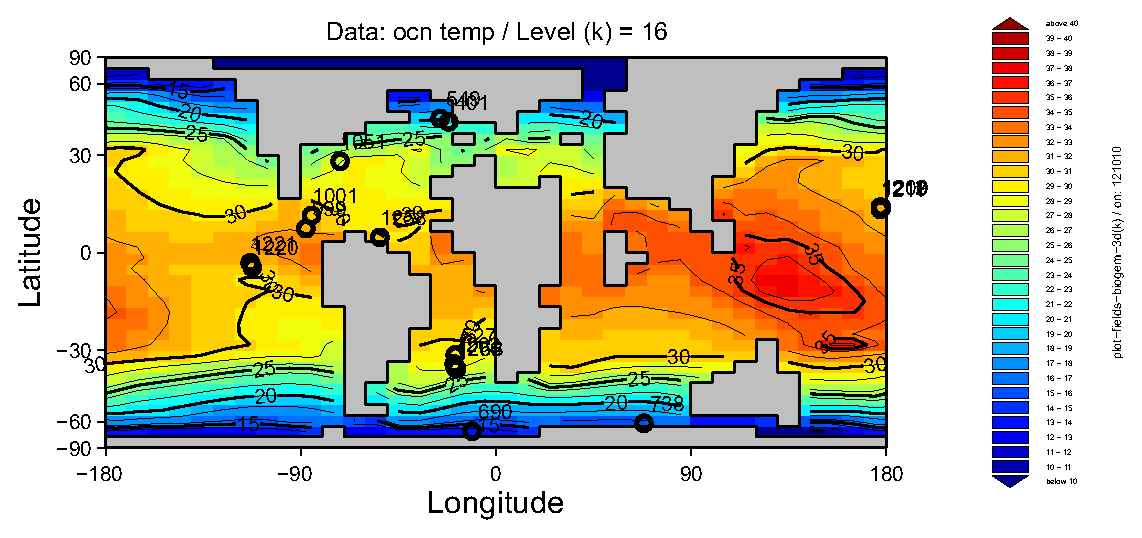
\includegraphics[scale=0.75]{cgenie_datalocations.eps}
\end{center}
\caption{Paleocene-Eocene deep-sea sediment drill locations together with a contour-overlain map of surface temperature.}
\label{fig:cgenie_datalocations}
\end{figure}

%------------------------------------------------

\subsection{Time-series plotting}

%------------------------------------------------

\subsection{Sediment model output analysis}

%----------------------------------------------------------------------------------------
%       CHAPTER X
%----------------------------------------------------------------------------------------

\cleardoublepage

\chapterimage{big-data.jpg} % Chapter heading image

\chapter{muffindata}

\hfill \break
\vspace{24mm}

%------------------------------------------------

\newpage

%------------------------------------------------

\section{Data re-gridding}

%------------------------------------------------

\newpage

%------------------------------------------------

\section{Miscellaneous data processing}

%----------------------------------------------------------------------------------------
%       CHAPTER X
%----------------------------------------------------------------------------------------

\cleardoublepage

%\chapterimage{Map_of_Earth_24.jpg} % Chapter heading image

\chapter{muffingen}

\hfill \break
\vspace{24mm}

%------------------------------------------------

\newpage

\section{muffingen basics}

%------------------------------------------------

\subsection{overview of the muffingen software}

\textbf{muffingen} is a collection of \textbf{MATLAB} functions that can create all the configuration files (excluding optional climatic and biogeochemical \textit{forcing} fields) required by the cGENIE (\textbf{muffin}) Earth system model. \textbf{muffingen} is designed to take the output from a fully coupled GCM, particularly of past climates with different continental configurations, and re-grid the output needed by the \textbf{muffin} model, in the form of files of boundary conditions, all  saved  in their respective correct format. However, \textbf{muffingen} can also be used to draw conceptual alternative Earths (in terms of continental configuration). Again, saving the required \textbf{muffin} files in their appropriate formats.

As a \textbf{MATLAB} code, (only) very basic familiarity with using \textbf{MATLAB} at the command line is required. And a copy/license of the \textbf{MATLAB} software ... A sufficient grasp of \textbf{MATLAB} can be gained by going through the following sections/subsections of the \textsf{matlabananas} textbook, which can be found on \href{https://github.com/derpycode/matlabananas}{GitHub} (look for the PDF file compiled form the latex source -- \textsf{BANANAS.pdf}):

\vspace{2mm}
\begin{itemize}[noitemsep]
\item Section 1.1 -- The \textbf{MATLAB} interface and command line.
\item Section 1.6 -- Changing directories and file search paths.
\item Section 2.2 -- Using \textit{functions} ... of which \texttt{muffingen} is one.
\end{itemize}
\vspace{2mm}

%------------------------------------------------

\subsection{Installing muffingen}

The \textbf{muffingen} code is hosted on GitHub:

\vspace{2mm}
\href{https://github.com/derpycode/muffingen}{\texttt{https://github.com/derpycode/muffingen}}
\vspace{2mm}

There are 2 ways to get your mitts on the \textbf{muffingen} code:

\vspace{2mm}
\begin{enumerate}

\vspace{1mm}
\item By downloading an archive file, containing all the code etc. For this -- click on the \textcolor[rgb]{0,0.501961,0}{green} \textsf{\small{Clone or Download}} button, and select \textsf{\small{Download ZIP}}.
\\You then unpack/unzip the files and directory structure where you want it.
\\This [archive download] is a perfectly workable way to proceed\footnote{Note that this way, you will be unable to easily update the code with whatever new developments or bug fixes occur in the future, nor can propagate back any code changes that you might have made and might want to become part of the official \textbf{muffingen} code  (i.e. downloading the \textsf{zip} file becomes a one-off installation that loses its formal connection to the GitHub repository).} ... 

\vspace{1mm}
\item Or you can \textit{clone} the repository to where you intend to run \textbf{muffingen}. Note that you will need a git client installed on your computer. There are GUI clients for git, or this can be done at the command line:

\vspace{-2mm}
\begin{verbatim}
$ git clone https://github.com/derpycode/muffingen.git
\end{verbatim}
\vspace{-2mm}

By doing this, you have created your own code repository (and an identical copy of the one hosted on GitHub). As part of the \texttt{git clone} command, you also automatically \textit{check out} (from your very own personal repository) a copy of the code.

\end{enumerate}
\vspace{2mm}

Note that you download or clone \textbf{muffingen} to the computer that you have \textbf{MATLAB} installed on and will use to run \textbf{muffingen} (i.e. not necessarily to the computer where \textbf{muffin} itself is run).

%------------------------------------------------

\newpage

\subsection{Running muffingen}

To use the \textbf{cGENIE.muffin} model configuration generator \textbf{muffingen} -- at the command line in \textbf{MATLAB}, simply type:

\vspace{-2mm}
\begin{verbatim}
>> muffingen('FILENAME')
\end{verbatim}
\vspace{-2mm}

\noindent where \texttt{FILENAME} is the name of an ASCII format configuration file (having a \texttt{.m} filename extension) that specifies the required settings (see subsequent section).

This file (\texttt{FILENAME.m}), must either be present in the directory where you installed \textbf{muffingen} (the directory where e.g. where the file \texttt{muffingen.m} is located) e.g. \textsf{C:\textbackslash muffingen}. In this case, your \textbf{MATLAB} working directory must also be  set to \textsf{C:\textbackslash muffingen}. Or, the \textbf{MATLAB} working directory and the file \texttt{FILENAME.m} can reside elsewhere (both directory locations must be the same however). In this case, you will then 'add' the location of \textbf{muffingen} to \textbf{MATLAB}'s search path by the \textbf{MATLAB} function \texttt{addpath}\footnote{Refer to the \textbf{MATLAB} '\textsf{bananas}' text for the syntax for using \texttt{addpath}.}.

The \textbf{muffingen} model configuration generator then starts, and depending on the specific settings in the configuration file, may require no user input, or may require user input, either because this option was requested, or because a re-gridding issue arose that requires manual intervention to resolve. A series of plots are created (and saved) as the configuration generation progresses together with the \textbf{muffin} model configuration files themselves. All the various steps plus details of how the contents of the configuration files are generated are reported at the command line, and saved in a n ASCII format \texttt{*.log} file for future reference.

Depending on the specific configuration file settings (see later), \textbf{muffingen} has 4 main modes of operation, which are summarized as follows (and described in more detail, along with specific examples, below):

\begin{enumerate}[noitemsep]
\setlength{\itemindent}{.2in}
\setcounter{enumi}{0}
\vspace{1mm}
\item \textbf{Configuration derivation based on re-gridding climate output from a GCM.}
\\ The most common usage of \textbf{muffingen}, and enabling a new (typically paleo) configuration to be derived from the output of a GCM experiment. Currently options for utilizing 4 different GCMs are provided: HadCM3(l), FOAM, CESM, and ROCKE-3D.
\vspace{1mm}
\item \textbf{Derivation based on an existing model topography ('\texttt{.k1}') file.}
\\ Allowing a topography to be re-created, or adapted/altered, all directly from an existing model 'k1' file (and hence existing model configuration).
\vspace{1mm}
\item \textbf{Derivation based on a prescribed land-sea mask.}
\\ This option will create a new configuration from any specified land-sea mask, whether 'real' or completely hypothetical.
\vspace{1mm}
\item \textbf{From a blank (all ocean) initial template.}
\\ Finally, this option enables a topography to be 'drawn' within \textbf{muffingen} and hence represents an interactive alternative to (3) (rather than editing a land-sea mask in a text editor).
\end{enumerate} 

%------------------------------------------------

\newpage

\section{Configuring muffingen}

%------------------------------------------------

When \textbf{muffingen} is run, a configuration file with a specified filename\footnote{i.e. the single parameter passed to \textbf{muffingen} when it is invoked at the command line} is loaded. The configuration file is in a simple plain text (ASCII) format, but is given a \textsf{.m} extension, enabling the values of a number of controlling parameter values to be set directly in \textbf{MATLAB}.\footnote{Note that the parameter filename is passed as a string without the .m extension (which is implicitly assumed). An error message will be generated if the file does not exist or has the incorrect extension.} The configuration file parameters control facets of \textbf{muffingen} behavior such as the primary model of operation, input and output filenames, what types of configuration files you want to generate, as well as there being a number of parameters controlling the finer details of re-gridding and configuration file generation, including whether to enable user-input or not.

The configuration files can be edited with the \textbf{MATLAB} editor (indeed, as a \textsf{.m} file, they are inherently a \textbf{MATLAB} format file), or any plain text (ASCII) editor. They must have a \textsf{.m} filename extension. 
The configuration file is divided up into sections of different parameter options. The main (most commonly used) parameters are summarized as follows (and are more fully described later):

\begin{itemize}

\vspace{4mm}
\item []
\small\vspace{-2pt}\begin{verbatim}
% *** CONFIG NAME AND MAIN INPUT SETTINGS *******************************
\end{verbatim}\vspace{-2pt}\normalsize

\vspace{2mm}
\begin{itemize}[noitemsep]

\vspace{1mm}
\item [] \texttt{par\_wor\_name}
\\Defines the name of the model configuration. This must be a string, 8 characters long.
\\e.g. \texttt{par\_wor\_name='my\_world'}

\vspace{1mm}
\item [] \texttt{par\_gcm}
\\Defines the format of the input. The string is blank for an interactive user-defined world, i.e. \texttt{par\_gcm=''}
\\See Section 16.1.3.

\vspace{1mm}
\item [] \texttt{par\_expid}
\\Defines the name of the GCM experiment if a GCM input is selected, or the '\textsf{.k1}' or '\textsf{.dat}' files if those respective input formats are selected by the above option.

\end{itemize}

\vspace{4mm}
\item []
\small\vspace{-2pt}\begin{verbatim}
% *** FILE PATHS ********************************************************
\end{verbatim}\vspace{-2pt}\normalsize

\vspace{4mm}
\item []
\small\vspace{-2pt}\begin{verbatim}
% *** GCM netCDF FILENAMES **********************************************
\end{verbatim}\vspace{-2pt}\normalsize

\vspace{4mm}
\item []
\small\vspace{-2pt}\begin{verbatim}
% *** GRID RESOLUTION ***************************************************
\end{verbatim}\vspace{-2pt}\normalsize

\vspace{2mm}
\begin{itemize}[noitemsep]

\vspace{1mm}
\item \texttt{par\_max\_i}
\\Defines the number of grid points in the longitude ('i') direction.
\\This is typically 36 or 18, e.g. \texttt{par\_max\_i=36}

\vspace{1mm}
\item \texttt{par\_max\_i}
\\Defines the number of grid points in the latitude ('j') direction.
\\This is typically 36 or 18 and is typically the same number as for the i direction, e.g. \texttt{par\_max\_j=36}

\vspace{1mm}
\item \texttt{par\_max\_k}
\\Defines the name of ocean layers.
\\This is almost always either 16 or 8, e.g. \texttt{par\_max\_k=16}

\vspace{1mm}
\item \texttt{opt\_equalarea} [default: \texttt{true}]
\\This specifies an equal area grid. (A value of \texttt{false} results in the latitude grid being in equal increments of latitude).

\end{itemize}

\vspace{4mm}
\item []
\small\vspace{-2pt}\begin{verbatim}
% *** REGRIDDING SETTINGS ***********************************************
\end{verbatim}\vspace{-2pt}\normalsize

\vspace{2mm}
\begin{itemize}[noitemsep]
\vspace{1mm}
\item [] \texttt{par\_max\_D} [default: \texttt{5000.0}]
\\Sets the maximum ocean depth (in m).
\end{itemize}

\end{itemize}

%------------------------------------------------

\newpage

\section{Configuring muffin model experiments}

%------------------------------------------------

Having created a new \textbf{muffin} configuration using the \textbf{MATLAB} function \texttt{muffingen}, carry out the following steps:

\vspace{2mm}
\begin{enumerate}

\vspace{1mm}
\item Firstly, copy/transfer the entire  configuration subdirectory (the directory with the same name as whatever you called your 'world')  and its contents, from the \textbf{muffingen} output directory (e.g. \textsf{muffingen/OUTPUT.EXAMPLES}) on your local computer, to:

\vspace{1mm}
\texttt{cgenie.muffin/genie-paleo}
\vspace{1mm}

\noindent on the computer that you run the \textbf{muffin} model on.

\vspace{1mm}
\item Create a new \textit{base-config} file. You do this by:
\begin{enumerate}
\vspace{1mm}
\item Taking one of the template \textit{base-config} files:
\vspace{-2pt}\begin{verbatim}
CONFIG_template_08lvl_R07.config
CONFIG_template_16lvl_C09.config
\end{verbatim}\vspace{-2pt}
The first being suitable for an 8-level (non seasonally forced ocean) and the second for a 16-level (seasonally forced) ocean.
\\Copy/rename the file to something ... 'appropriate' ... remembering: no spaces are allowed in the filename, and you need to retain the \textsf{.config} file extension.
\vspace{1mm}
\item There is a highlighted (\(<<<\;\;\;\;\;>>>\)) line in the template \textit{base-config} file:
\footnotesize\vspace{-2pt}\begin{verbatim}
# *******************************************************************
# GRID & BOUNDARY CONDITION CONFIGURATION
# *******************************************************************
# insert the automatically generated muffingen parameter list here
# *******************************************************************
# <<<                                                             >>>
# *******************************************************************
\end{verbatim}\vspace{-2pt}\normalsize
Copy and past the contents of the \textbf{muffingen} output file\footnote{In the filename, \texttt{yymmdd} is the date of the configuration creation.}:
\vspace{-2pt}\begin{verbatim}
config_yymmdd.txt
\end{verbatim}\vspace{-2pt}
into the template file where indicated (immediately above, immediately below, or simply replacing the (\(<<<\;\;\;\;\;>>>\)) line.
\vspace{1mm}
\item Now copy this new \textit{base-config}, to:
\vspace{-2pt}\begin{verbatim}
cgenie.muffin/genie-main/configs
\end{verbatim}\vspace{-2pt}
\end{enumerate}

\noindent Note that in using one of the template \textit{base-config} files, you have configured an ocean with just 2 tracers -- temperature and salinity (i.e., there is no carbon cycle or ocean nutrients \textit{etc.} enabled at this point).

\vspace{1mm}
\item Create a new \textit{user-config} file to complete the experimental setup.

\noindent An example/template \textit{user-config} file (designed for climate-only simulations) is also provided in the main \textbf{muffingen} directory:

\vspace{1mm}
\texttt{EXAMPLE.SPIN}

\vspace{1mm}

Rename and copy this (or copy and rename) to \textbf{muffin} model directory:

\vspace{1mm}
\texttt{genie.muffin/user-configs}
\vspace{1mm}

\end{enumerate}
\vspace{2mm}

%------------------------------------------------

\newpage

\section{muffingen parameter settings details}

***UNDER\ CONSTRUCTION ...***




\subsubsection{Zonal wind-stress}

For non GCM-based configurations, no prior wind fields exist. \textbf{muffingen} hence creates and configures an idealized zonal wind-stress field (from which wind velocity and wind speed is derived). The zonal wind-stress can take alternative strengths, depending on whether a high latitude gateway (in either hemisphere) exists. This can be prescribed directly, or \textbf{muffingen} can be enabled to 'choose' whether or not a high latitude gateway exists and hence whether or not to apply a strong or weak zonal flow. The parameter options (in the \textbf{muffingen} configuration file) are:

\begin{itemize}
\item \texttt{par\_tauopt=0;}
\\\textbf{muffingen} chooses whether or not to apply a strong or weak zonal flow, and in which hemisphere.
\item \texttt{par\_tauopt=1;}
\\A weak zonal flow is applied in both hemispheres.
\item \texttt{par\_tauopt=2;}
\\A strong zonal flow is applied in both hemispheres.
\end{itemize} 

For reference -- the modern world has a mix of strong (southern) and weak (northern) hemisphere zonal flows.

The different EXAMPLE (\small\textsf{.m}\normalsize) configuration files have a mixture of default choices:

\begin{itemize}
\item \small\textsf{muffingen\_settings\_BLANK}\normalsize, 
\\\small\textsf{muffingen\_settings\_drakeworld}\normalsize, 
\small\textsf{muffingen\_settings\_eqpasworld}\normalsize, 
\\\small\textsf{muffingen\_settings\_ridgeworld}\normalsize, 
\small\textsf{muffingen\_settings\_waterworld}\normalsize:
\\\texttt{par\_tauopt=0;}
\item \small\textsf{muffingen\_settings\_wppcont1}\normalsize:
\\\texttt{par\_tauopt=2;}
\item \small\textsf{muffingen\_settings\_modern}\normalsize:
\\n/a (wind-stress derived from GCM fields)
\end{itemize}

\noindent (No EXAMPLE configurations currently specify a strong zonal field, although \\\small\textsf{muffingen\_settings\_ridgeworld }\normalsize will be prescribed one automatically in \textbf{muffingen}.) 

%------------------------------------------------

\newpage

\section{muffingen configuration examples}

A series of example configurations are provided in the main \textbf{muffingen} directory:

\vspace{1mm}
\begin{itemize}[noitemsep]
\vspace{1mm}
\item \texttt{muffingen\_settings\_BLANK} -- Starts from a blank ('water-world') all-ocean land-sea mask template.  User input (allowing continents and seafloor topography to be 'drawn') is activated by default.
\vspace{1mm}
\item \texttt{muffingen\_settings\_wppcont1} -- Starts from a land-sea mask: \footnotesize\textsf{wppcont1.dat}\normalsize, which is stored in the \textbf{muffingen} subdirectory \footnotesize\textsf{INPUT.EXAMPLES}\normalsize. The mask defines an idealized pole-to-pole super-continent. There is no user input by default (so no modifications can be made, by default), but this can be enabled (\texttt{opt\_user=true}).
\vspace{1mm}
\item \texttt{muffingen\_settings\_drakeworld} -- The first of a series of 4 conceptual worlds (loosely following the literature). As per \footnotesize\textsf{muffingen\_settings\_wppcont1}\normalsize, this tarts from a land-sea mask (\footnotesize\textsf{wordrake.dat}\normalsize) which is stored in the \textbf{muffingen} subdirectory \footnotesize\textsf{INPUT.EXAMPLES}\normalsize. The land fraction is minimal (as it is trying to reproduce the sort of zero-area numerical barrier used in the literature). This configuration has a barrier to ocean circulation, from the N pole down, with a high southern latitude gateway (a Drake Passage like feature). 
\vspace{1mm}
\item \texttt{muffingen\_settings\_eqpasworld} -- As above, except with an equatorial (only) gateway.
\vspace{1mm}
\item \texttt{muffingen\_settings\_ridgeworld} -- As above, except with no gateway.
\vspace{1mm}
\item \texttt{muffingen\_settings\_waterworld} -- As above, but with no barriers, i.e. a 'water world'.
\vspace{1mm}
\item \texttt{muffingen\_settings\_wor0251b1} -- Start from a muffin model configuration 'k1' topography defining file: \texttt{p0251b.k1}, which is stored in the \textbf{muffingen} subdirectory \texttt{INPUT.EXAMPLES}. The k1 file defines a late Permian continental configuration (and bathymetry). There is no user input by default (so no modifications can be made, by default), but this can be enabled (\texttt{opt\_user=true}).
\vspace{1mm}
\item \texttt{muffingen\_settings\_modern} -- Takes the continental configuration and climate simulation output from a fully coupled GCM experiment (files in directory \footnotesize\textsf{xbowl }\normalsize in the \textbf{muffingen} subdirectory \footnotesize\textsf{INPUT.EXAMPLES }\normalsize) and derives full \textbf{muffin} model boundary conditions. User input (allowing continents and seafloor topography to be 'edited') is activated by default.
\end{itemize}
\vspace{2mm}

\noindent These examples span the 4 main ways of using \textbf{muffingen} (as summarized earlier),  and which are described in detail in following sections:

\vspace{1mm}
\begin{enumerate}[noitemsep]
\vspace{1mm}
\item \textbf{From a blank (all ocean) initial template.}
\\ Finally, this option enables a topography to be 'drawn' within \textbf{muffingen} and hence represents an interactive alternative to (3) (rather than editing a land-sea mask in a text editor).

\vspace{1mm}
\item \textbf{Derivation based on a prescribed land-sea mask.}
\\ This option will create a new configuration from any specified land-sea mask, whether 'real' or completely hypothetical.
\vspace{1mm}
\item \textbf{Derivation based on an existing model topography ('\texttt{.k1}') file.}
\\ Allowing a topography to be re-created, or adapted/altered, all directly from an existing model 'k1' file (and hence existing model configuration).
\vspace{1mm}
\item \textbf{Configuration derivation based on re-gridding climate output from a GCM.}
\\ The most common usage of \textbf{muffingen}, and enabling a new (typically paleo) configuration to be derived from the output of a GCM experiment. Currently options for utilizing 4 different GCMs are provided: HadCM3(l), FOAM, CESM, and ROCKE-3D.
\end{enumerate} 
\vspace{2mm}

%------------------------------------------------

\subsection{overview of the muffingen software}



%------------------------------------------------
%
%----------------------------------------------------------------------------------------
%       CHAPTER X
%----------------------------------------------------------------------------------------

\cleardoublepage

\chapterimage{chx-cheerilee.png} % Chapter heading image

\chapter{FAQ}

\hfill \break
\vspace{24mm}

\noindent \huge \textbf{\textit{aka}: 'Has this dumb question been asked before?'}\normalsize

%------------------------------------------------

\newpage

%------------------------------------------------

\section{Installation related questions}

%------------------------------------------------
%

\subsubsection{Stack space}

You may encounter issues with regards to the \texttt{ifort} Intel FORTRAN compiler (an maybe others), particularly when using SEDGEM because of the size of the arrays holding sediment information:

\vspace{2mm}
\noindent ''\textit{The Intel® Fortran Compilers 8.0 or higher allocate more temporaries on the stack than previous Intel Fortran compilers.
Temporaries include automatic arrays and array sub-sections corresponding to actual arguments. If the program is not afforded adequate stack space at runtime relative to the total size of the temporaries,
the program will terminate with a segmentation fault.}''

\vspace{2mm}
\noindent The (a?) solution is to increase the CPU stack space, Try:
\vspace{-2pt}\begin{verbatim}$ ulimit -s unlimited\end{verbatim}\vspace{-2pt}

%------------------------------------------------

\newpage

%------------------------------------------------

\section{Cluster/queue questions}

%------------------------------------------------
%
\subsubsection{Do I have to submit experiments to the queue rather than running interactively?}

\textbf{Yes!} Except for developing the model and debugging, testing new experimental designs, and forcing a re-compile. The number of instances of the model that can be run simultaneously interactively is limited by the number of processing cores on the head node. The more experiments that are run interactively, the slower everything will go. Additionally, if you even temporarily lose your Internet connection, an interactively-run experiment will die. The queue is there for your convenience, believe it or not ...

%------------------------------------------------
\subsubsection{Can I leave all my experiment results on the cluster for ever?}

\textbf{No!} \uline{Nothing} is backed up on the cluster, and space is not infinite. So, periodically, transfer archived (\texttt{.tar.gz}) results off of the cluster and delete both the archive file and the results directory.

%------------------------------------------------

\newpage

%------------------------------------------------

\section{Help! My experiment has died ... why?}

%------------------------------------------------
%

If, when using the \textsf{\footnotesize runmuffin.sh} shell script to run a \textbf{cgenie.muffin} experiment, it all goes horribly pear-shaped ... 
\vspace{1mm}
\begin{enumerate}
   
\vspace{1mm}
\item The experiment dies absolutely immediately.
\\Check that the \textsf{\footnotesize runmuffin.sh} shell script has executable permissions. Also check that the directory you are trying to run the model from is the \textsf{\footnotesize genie-main} directory.
        
\item The experiment does not quite die immediately, but does not manage to stagger even as far as the line:
\vspace{-4pt}\begin{verbatim}
>> Here we go ...
\end{verbatim}\vspace{-4pt}
before dropping dead. If so, there should be an error message telling you that a particular file or directory cannot be found. Check:
        
\begin{itemize}
\item All the files and directories you have specified exist.
\item You have not omitted spaces where you should not have, nor added spaces where a '\texttt{\_}' separator was required.
\item You have not misspelt anything -- a common cause of problems is in reading the number one ('\texttt{1}') for the letter el ('\texttt{l}'), or \textit{vice versa} in the computer font (\texttt{Courier}).
\end{itemize}
        
\end{enumerate}
\vspace{2mm}

\noindent These first two sorts of pain and suffering are due to mis-configuration of the \textsf{\footnotesize runmuffin.sh} shell script. Also refer back to the overall sequence of configuring and running the \textbf{cGENIE.muffin} model shown in Figure \ref{fig:chx-jobcreation}.

%------------------------------------------------

\subsection{Other sources of error}

\noindent Other sources of error are due to the configuration of \textbf{cGENIE.muffin} (or more rarely, due to the model itself):
                
\vspace{1mm}
\begin{enumerate}

\vspace{1mm}
\item As \textbf{cGENIEmuffin} initializes, files may be reported as not being found. One possible cause of this is that '\texttt{\~{}}' may not necessarily get expanded into the path of your home directory (e.g., '\texttt{/home/mushroom}'. In this situation, '\texttt{\~{}}' can simply be replaced with '\texttt{\$HOME}'. Note that as well as making this substitution at the command line, the \textit{user-config} file may also contain instances of '\texttt{\~{}}' (such as in specifying particular \textit{forcings}).
        
\vspace{1mm}
\item A missing/not found error can also arise with some compilers if one of the various ASCII input files to \textbf{BIOGEM} (or \textbf{SEDGEM}) does not have a blank line at the bottom (some vague quirk of the unformatted read used in the \textbf{FORTRAN} code). Check: the \textit{user-config} file, and also any boundary condition files being requested.
        
\vspace{1mm}
\item Further trouble can occasionally arise when using \textbf{Windoz} and editing files (e.g., the \textit{user-config} file) and it is possible to corrupt the format of the file. For what file(s) you have edited, use the command \texttt{dos2unix} to strip off \textbf{Windoz} formatting characters (which are invariably invisible in most editors). The syntax for this (or see the \textbf{linux} 'man' pages, or even Google it) is \texttt{\$ dos2unix FILENAME}.
        
\vspace{1mm}
\item If the model starts running, but dies with a reported failure to solve the aqueous carbonate system, it may be that you need to force a re-compile (\texttt{\$ make cleanall}). Running \textbf{cGENIE.muffin} with array dimensions which do not match the number of tracers selected is a common cause of failures to solve the aqueous carbonate system, as often calcium ion or other tracer concentrations become corrupted and get assigned nutty and all but impossible values.
\\Also, if a \textit{re-start} is used which was generated with a different land-sea mask (and \textit{base-config}) to the current experiment and associated \textit{base-config}. Try running without the \textit{re-start} and see if that solves it (identifies the source of the problem).

\end{enumerate}
\vspace{2mm}

%------------------------------------------------

\subsection{Meaning of specific error messages}

\vspace{2mm}
\subsubsection{'ERROR: path integral around island too long'}

Such an error is possible when developing new or modifying existing continental configurations (and associated 'island' and 'path' definition files), but not in normal running of the model.
First try a \texttt{make cleanall} and then try re-running.
If the problem persists, it is possible that a key configuration file has accidently/somehow been changed. To check for this -- do a \texttt{make cleanall}, and then from the \textsf{\footnotesize cgenie.muffin} directory:
\vspace{-2pt}\begin{verbatim}
svn status -u
\end{verbatim}\vspace{-2pt}
Any file that you have modified is labeled with an \texttt{m}. Any new files on the server that you don't have will have a \texttt{*}. Files with a \texttt{?} are files that exist locally and are not on SVN (and can be ignored).
If there is a file with an \texttt{m} that should not have been modified:
\vspace{-2pt}\begin{verbatim}
svn revert FILENAME
\end{verbatim}\vspace{-2pt}
will re-set the file \texttt{FILENAME} (also include the relative path) it to the current SVN version status.

\vspace{2mm}
\subsubsection{'ERROR MESSAGE: Particulate tracer CaCO3 ...'}

I have been told '\texttt{ERROR MESSAGE: Particulate tracer CaCO3 does does not have the corresponding ocean tracer Ca selected}' -- is this a problem ... ?

\textbf{No!} You are simply being reminded that you have calcium carbon (CaCO$_{3}$) selected as a particulate tracer in the model, but although when it dissolves it releases Ca$^{2+}$ (and removes Ca$^{2+}$ when CaCO$_{3}$ is precipitated), you do not have Ca$^{2+}$ selected as an explicit dissolved tracer in the ocean. This is not a problem as by far the most important effect on the carbon cycle of adding/subtracting Ca2+ is a change in alkalinity, which is implicitly account for. Only on \textbf{very} long time-scales, or in deep-time situations when the Ca$^{2+}$/Mg$^{2+}$ ratio was very different form today, might you need to select Ca$^{2+}$ (and Mg$^{2+}$) as an ocean tracer.

%------------------------------------------------

\newpage

%------------------------------------------------

\section{General running and configuring experiments questions}

%------------------------------------------------
%
\subsubsection{When does the model need to be recompiled?}

\textbf{cGENIE.muffin} will need to recompile in the following situations:

\begin{itemize}

\vspace{1mm}
\item You have just carried out one of the \textbf{cGENIE.muffin} tests, e.g., \texttt{make test} or \texttt{make testbiogem}.
\item You have changed the dimension of the climate model grid (which also means an automatic change in the biogeochemistry modules), either horizontally (e.g., going from \(36\times 36\) to \(18\times 18\)) or vertically (e.g., going from \(8\) levels in the ocean to \(16\)).
\item You have changed the number of selected ocean biogeochemical tracers in the \textit{base-config} and hence changed the value of:
\small\begin{verbatim}
GOLDSTEINNTRACSOPTS='$(DEFINE)GOLDSTEINNTRACS=2'
\end{verbatim}\normalsize

\end{itemize}
(The latter two involve a change in compiled array dimension.)

In all three situations, the \textit{base-config }is being changed (or should be\footnote{One could edit a \textit{base-config} and re-ruin, but it is better to create a new \textit{base-config }file if editing any of the settings, particularly those affecting array dimensions}). In running at the command line (i.e. interactively), the \texttt{\footnotesize runmuffin.sh} script detects the change in base-config, and automatically forces a re-compile for you. However, the compute nodes of the cluster do not have access to the \textbf{FORTRAN} compiler. As a sad and unfortunate consequence, submitted jobs cannot recompile modules and all science modules must be already compiled when a job is submitted.\footnote{It is OK to change the flavor of GENIE as linking is done by the C compiler.}

To  recompile (and re link) the science modules -- first, start an interactive run of the experiment you want to conduct. This will ensure that it is correctly compiled. This also serves as a visual check that you have requested a \textit{user-config}, restart, etc that actually exists. Start the run for the length of time you intend to use when submitting the experiment as a job to the queue, but kill it (keyboard command: \textsf{\footnotesize Ctrl-C}) once it is compiled and you are happy that it is running OK (say, after 10 years).
\noindent You can now be reasonably confident that the experiment is safe to submit the job to the cluster (and all files and inputs are as they should be).

If you have multiple experiments, all with the same resolution and number of tracers, you DO NOT need to re-run interactively or attempt to recompile. Also, you can add 'modules' and not recompile. i.e., you can interactively run an ocean -only carbon cycle. And then submit it. And then submit an experiment using \textbf{SEDGEM} as well. (Because when the model is compiled, ALL sciences modules are compiled, meaning that all there is to do is just link them, which does not require the (\texttt{ifort}) \textbf{FORTRAN} compiler.)

Refer to Figure \ref{fig:chx-jobcreation} for the sequence of steps associated with configuring and running model experiments.

%------------------------------------------------
%
\subsubsection{In the naming of different \textit{forcing} specifications: what does '\texttt{yyyyz}' mean?}

\textbf{A.} The naming convention for \textit{forcings} is that the (sub)directory name starts with the code for the continental configuration, if the \textit{forcing} is tied to a specific continental configuration. For example: \textit{forcings} with the string '\textsf{\footnotesize FeMahowald2006}' relate to the prescription of a dust (Fe flux) field re-gridded from \textit{Mahowald et al.} [2006]. When this has been re-gridded to the \textsf{\footnotesize worjh2} continental configuration, \textsf{\footnotesize worjh2} appears at the start of the name. If the \textit{forcing} is independent of a specific continental configuration, such as restoring atmospheric \(CO_{2}\) to a prescribed value (uniformly throughout the atmosphere), the string is '\textsf{\footnotesize yyyyz}', as in e.g.: \textsf{\footnotesize pyyyyz\_Rp\(CO_{2}\)\_Rp13\(CO_{2}\)}.

%------------------------------------------------
%
\subsubsection{Can I make the model run faster?}

*sign* You speed freak. Is this all you care about? What about the quality of the simulation - does that mean absolutely nothing to you? Oh well ...
There is a bunch of stuff that slows \textbf{cGENIE.muffin} down that may not be absolutely essential to a particular model experiment. These include:

\begin{itemize}[noitemsep]
\setlength{\itemindent}{.2in}

\item   The number of tracers - if you don't need 'em, then don't select 'em! Selected tracers are automatically passed to \textbf{GOLDSTEIN} and advected/convected/diffused with ocean circulation. Similarly, \textbf{BIOGEM} does a whole bunch of stuff with tracers, particularly those which can be biologically transformed. All this is numerically wasteful if you aren't interested in them. Equally importantly, the more tracers you have selected the more careful you have to be in configuring the model. Superfluous tracers therefore cost more configuration time and/or increase the change of a model crash.

\item \textit{Tracer auditing} - the  continuous updating and checking global tracer inventories to ensure that there is no spurious loss or gain of any tracer (i.e., a bug) has computational overheads associated with it. Whether this checking is carried out or not is set by the value of the flag \texttt{bg\_ctrl\_audit}\footnote{It is \texttt{.false.} by default.}.

\item \textit{Time-series} results saving. Model tracer (plus some physical) properties are bring continuously averaged in constructing \textit{time-series} results files. Cutting down on \textit{time-series} that you don't need will help minimize model run-time. The various categories of time-series that will be saved are specified by a series of namelist parameter flags. However, within each category (such as \texttt{ocn} tracers - \texttt{bg\_ctrl\_data\_save\_sig\_ocn}) all properties will be saved - you are not given to option to save a defined sub-set (for example, \(DIC\) and \(PO_{4}\) in the ocean but not \(ALK\)).

\item Time-slice results saving. If you have relatively few requested time-slices over the course of the model integration then this is unlikely to significantly impact the overall run-time (even will all possible data category save namelist flags set to \texttt{.true.}). However, note that if you have accidently triggered the default time-slice saving interval (by having no data items in the time-slice specification file (\texttt{bg\_par\_infile\_slice\_name}) you may end up with the model running about as fast as a 2-legged dog super-glued to a 10-tonne biscuit.

 Note that time-series saving of data that is a 2-D average, such as atmospheric composition at the ocean-atmosphere interface, sediment composition at the ocean-sediment interface, or just ocean surface conditions, is less numerically demanding than mean values that have to be derived from a 3-D data field.

\item Alter the degree of synchronicity between climate and biogeochemistry (see  HOW-TO guide).

\end{itemize}

\vspace{2mm}
As a very rough guide, the impact on total run-time of making various changes to the model configuration are listed as follows. Numbers are given as a percentage increase in total model run-time (using the /usr/bin/time linux command). Tracers selected in the ocean are DIC, ALK, PO4, O2, DOM\_C, DOM\_P, DOM\_O2, as well as 13C isotopic components (DIC\_13C and DOM\_C\_13C) (+ T and S). The corresponding tracers are present in the atmosphere and as particulates. The model is run for 10 years as a new run (i.e., not loading in a restart file):

\begin{itemize}[noitemsep]
\setlength{\itemindent}{.2in}

\item   ADD auditing \begin{math}\Rightarrow\end{math} +15\%
\item   ADD time-slice saving   \begin{math}\Rightarrow\end{math} +20\%\footnote{Because only a 10 year integration has been carried out with a time-slice saved at 10 years, the computational cost of time-slice saving is disproportionately high as displayed. With a longer integration, the relative cost of saving a time-slice will fall. In contrast, the computational cost as a fraction of total run-time of time-series saving and auditing is likely to remain the same.}
\item   ADD time-series saving  \begin{math}\Rightarrow\end{math} +15\%
\item   REMOVE \begin{math}^{13}\end{math}C isotopic species (= DIC and DOC ocean tracers) \begin{math}\Rightarrow\end{math} -10\%\footnote{The speed gained by removing two tracers is not proportional to the fractional decrease in number of tracers (in this example reducing from 11 to 9 the number of tracers in the ocean gives only a ca. 10\% improvement in overall speed).}

\end{itemize}

\vspace{2mm}
You can also run at lower resolution. The basic configuration for a faster 'lego box' \textbf{cGENIE.muffin} configuration consists of a \(18\times 18\) model grid and an \(8\) level ocean. The continents are in a zonally-averaged configuration and there is no topography in the oceans.

The model is accelerated by:

\begin{enumerate}[noitemsep]
\setlength{\itemindent}{.2in}
\item it's low resolution
\item taking \(48\) instead of \(96\) ocean time-steps per year in the ocean
\item \textbf{BIOGEM} being only being updated every \(4\) rather than every \(2\) ocean time-steps.
\end{enumerate}

In this configuration 100 years take about 40 seconds, 10 kyr would just take over and hour, and 100 kyr could be run overnight!

%------------------------------------------------

\newpage

%------------------------------------------------

\section{Climate-y questions}

%------------------------------------------------
%
\subsubsection{Can I disable climate feedback with \(CO_{2}\)?}

Yes, for instance when you might want to compare the fate of \(CO_{2}\) released to the atmosphere with climate (and ocean circulation and temperatures) not responding, vs. \(CO_{2}\) in the atmosphere also driving changes in climate (and hence affecting the pathways and transformations of \(CO_{2}\), particularly in the ocean).

\vspace{2mm}
To specify no climate feedback, add to the \textit{user-config} file:
\vspace{-2mm}\small\begin{verbatim}
# set no CO2 climate feedback
ea_36=n
\end{verbatim}\normalsize\vspace{-2mm}
as well as a radiative forcing scaling:
\vspace{-2mm}\small\begin{verbatim}
# scaling for atmospheric CO2 radiative forcing, relative to 278 ppm
ea_radfor_scl_co2=1.0
\end{verbatim}\normalsize\vspace{-2mm}
(a value of \texttt{1.0} giving no change in climate relative to the default).

%------------------------------------------------
%
\subsubsection{How do I change the orbital configuration of cGENIE.muffin?}

[see Orbits HOW-TO]

%------------------------------------------------
%
\subsubsection{Can I do solar geoengineering (SRM) experiments?}

No! Because you might destroy the planet.

\noindent No wait ... in the model (world) ... yes! But because of the absence of a dynamical atmosphere, options here are limited. However, modification of the solar constant, \textit{a-la} 'giant mirrors in space' is possible. Sea-ice (surface) albedo can also be adjusted.

%------------------------------------------------

\newpage

%------------------------------------------------

\section{Ocean biogeochemistry questions}

%------------------------------------------------
%
\subsubsection{Can  solubility related changes be separated from stratification and circulation changes?}

With \textbf{BIOGEM} coupled to the climate model core of \textbf{cGENIE.muffin} \footnote{Namelist: \texttt{ea\_36='y'}}, a change in atmospheric \(CO_{2}\) will induce a change in SSTs, which in turn affect the carbon cycle and feedback on \(CO_{2}\) via changes in solubility and via changes in circulation (stratification) and thus biological productivity. There are times when is it helpful to separate out solubility related changes from circulation related changes. This equally applies to dissolved \(O_{2}\) and \(CO_{2}\). The problem is that you need a change in climate and surface temperatures in the climate model in order to induce a change in circulation.

There is a way of having an altered climate and circulation, which then affects the marine carbon cycle, yet specify the SSTs that are actually seen by \textbf{BIOGEM} (and thus used in solubility calculations).

First of all, control the radiative forcing of climate internally in the \textbf{EMBM} rather than externally by the atmospheric \(CO_{2}\) concentration calculated by \textbf{ATCHEM}. Turn off explicit \(CO_{2}\) forcing of climate by setting: \texttt{ea\_36='n'}. The namelist parameter \texttt{ea\_20} will then dictate the EMBM radiative forcing: a value of \(1.0\) (default) gives no change in radiative forcing (\(CO_{2}\) = 278 ppm), a value of \(2.0\) corresponds to the effect of doubling \(CO_{2}\), \(\times  4\;CO_{2}\), etc. Altering the value of \texttt{ea\_20} thus lets you control climate (and circulation) without having to adjust \(CO_{2}\) and the carbon cycle.

Next, SSTs in \textbf{BIOGEM} can be specified independently of the climate model. You achieve this by setting up a restoring forcing of ocean temperatures at the surface. Note that by default, prescribing SSTs (or SSSs) in \textbf{BIOGEM} does not propagate through to the climate model which does its own independent climate thing based on the value of \texttt{ea\_20}. This allows you to retain the surface temperatures and thus solubility associated with a \(\times  1\;CO_{2}\) World, but have a warmer more stratified ocean (appropriate for a much warmer World).

What actually happens is that BIOGEM receives both the altered circulation field and the altered SSTs due to \(\times  4\;CO_{2}\), but sets its own SSTs internally rather than use those calculated by the climate model. Setting up the SST restoring is in principal just like for PO4. The values for the SST field you can simply copy and paste out of a prior \(\times  1\;CO_{2}\) experiment.

The converse experiment, is to have circulation and biological productivity not change, but explore the effect of changes in SST-driven solubility. i.e., to separate the solubility pump from circulation change effects on glacial \(CO_{2}\).

%------------------------------------------------
%
\subsubsection{What is the difference between the different Fe configurations and schemes?}

There is a parameter -- \texttt{bg\_opt\_geochem\_Fe} -- that specifies the Fe scheme (although note that you have to have the appropriate/required tracers selected):

\begin{enumerate}[noitemsep]
\setlength{\itemindent}{.2in}

\item \texttt{bg\_opt\_geochem\_Fe = 'OLD'}

This is the very original scheme, based on 3 tracers -- Fe (free dissolved Fe), FeL (ligand-bound Fe), and L (free ligand).

During scavenging, a new equilibrium partitioning between the 3 species is calculated and imposed on tracer concentrations via the remin array, but only at the surface.

Entrains some completely unnecessary accounting for Fe addition at the surface as part of the equilibrium calculation, including a call to \texttt{sub\_calc\_geochem\_Fe} as part of the main (i,j) biogem subroutine array. All other schemes are free from this.

\item \texttt{bg\_opt\_geochem\_Fe = 'ALT'}

This is also based on 3 tracers -- Fe (free dissolved Fe), FeL (ligand-bound Fe), and L (free ligand).

During scavenging, a new equilibrium partitioning between the 3 species is calculated and imposed on tracer concentrations via the remin array. This is carried out throughout the water column.

\item \texttt{bg\_opt\_geochem\_Fe = 'FeFe2LFeL'}

Based on the same 3 tracers -- Fe (free dissolved Fe), FeL (ligand-bound Fe), and L (free ligand),  but also, Fe2, which is ignored for the purposes of calculating scavening and Fe-FeL-L partitioning. Here, the tracer Fe is explicitly taken to be \(Fe^{3+}\).

Scavenging and tracer concentration re-partitioning as per (2).

\item \texttt{bg\_opt\_geochem\_Fe = 'hybrid'}

This is based on the minimum  number of tracers required to describe the system -- TFe (total dissolved Fe) and TL (total dissolved ligand). The equilibrium partitioning between Fe, FeL, and L, is derived when required.

\item \texttt{bg\_opt\_geochem\_Fe = 'lookup\_4D'}

Also based on TFe (total dissolved Fe) and TL (total dissolved ligand), but with Fe calculated via a lookup table.

\end{enumerate}

In schemes 1+2+3, scavenged Fe is removed form the Fe tracer pool. For 4+5, scavenged Fe is removed from the TFe pool.


%------------------------------------------------
%
\subsubsection{What is 'tracer auditing' -- should I have it switched on?}

When developing a new model parameterization, it is of fundamental importance that careful track is kept of the total tracer inventory of the system in the face of internal mass transfer and any inputs (e.g., prescribed restoring or flux boundary conditions) or outputs (e.g., sedimentation). No spurious gain or loss of tracer mass must occur as a result of bugs introduced to the code. The tracer inventories of the ocean can be periodically calculated and compared to that predicted to have occurred on the basis of any net input (or output) occurring in the intervening time to help catch bugs. The simplest implementation would be an audit carried out at system start-up (before any transformation of tracer mass has taken place), and at the very end (after the last transformation of the tracer fields). However, integrating over over an extended time period can lead to the excessive accumulation of numerical (truncation) errors. Instead, the audits are carried out periodically during the model run. The periodicity of tracer auditing follows the times specified for time-series data saving (i.e., at time listed in the file specified by \texttt{bg\_par\_infile\_sig\_name}).

The entire audit procedure is as follows:

\begin{enumerate}[noitemsep]
\setlength{\itemindent}{.2in}

\item First, an initial inventory is calculated, achieved by summing the product of the concentration of each (selected) tracer with the mass of each each cell, across all wet cells.
\item During the model run, the net spatially- and time-integrated transfer of tracer mass arising from all transfers across the external reservoir boundaries is calculated. 
\item At a periodic pre-defined time, the inventories are re-calculated. The difference between old and new inventories should be equal to the integrated net flux. If the relative difference between re-calculated inventory and estimated (on the basis of net flux) differs by more than a predefined threshold then an error message is raised (and the model halted if requested)
\item The integrated net flux variable is re-set to zero and steps (2-4) repeated.

\end{enumerate}

In short -- if you are not modifying the code then you can take it on trust(!) that the model distribution is free of (major) bugs and that spurious gain or loss of tracers does not occur. It you don't trust me ... then switch the auditing feature on.

Auditing is inactivated by default. To activate it:
\vspace{-2mm}\small\begin{verbatim}
bg_ctrl_audit = .true.
\end{verbatim}\normalsize\vspace{-2mm}

To adjust the threshold (relative) tolerance\footnote{By default, this is set to \texttt{1.0E-08}.}:
\vspace{-2mm}\small\begin{verbatim}
bg_par_misc_audit_relerr = value
\end{verbatim}\normalsize\vspace{-2mm}

To halt the model\footnote{By default the model will continue running, even if there is an apparent spurious drift in tracer inventories occurring.} if it fails the tracer drift tolerance:
\vspace{-2mm}\small\begin{verbatim}
bg_ctrl_audit_fatal = .true.
\end{verbatim}\normalsize\vspace{-2mm}

A secondary benefit of tracer auditing when running the model interactively, is that it reports back to you the maximum and minimum value of all the tracers (and locations of where this occurs), as follows:

\vspace{-2mm}\footnotesize\begin{verbatim}
 >>> SAVING BIOGEM TIME-SERIES @ year  0.50  278.069  -6.501  16.522  3.843  18.543  ...
     temp             / min = 0.2713E+03 (18,36, 8) / max = 0.3030E+03 ( 4,18, 8)
     sal              / min = 0.3337E+02 (10,35, 8) / max = 0.3891E+02 (30,29, 8)
     DIC              / min = 0.1878E-02 (35,24, 8) / max = 0.2581E-02 (33,21, 1)
     DIC_13C          / min = -.4225E+00 ( 3,16, 3) / max = 0.2792E+01 (25,13, 8)
     DIC_14C          / min = -.1779E+03 (33,21, 1) / max = 0.2197E+02 (30,29, 8)
     PO4              / min = 0.7071E-07 (29,28, 8) / max = 0.3806E-05 ( 3,16, 3)
     O2               / min = -.4521E-04 (27,30, 5) / max = 0.3363E-03 (24,35, 8)
     ALK              / min = 0.2212E-02 (10,35, 8) / max = 0.2724E-02 (33,21, 1)
     DOM_C            / min = -.4159E-05 (21,34, 3) / max = 0.1517E-04 (32,25, 8)
     DOM_C_13C        / min = -.1000E+20 ( 1, 3, 2) / max = 0.5817E+01 (29,36, 8)
     DOM_C_14C        / min = -.1000E+20 ( 1, 3, 2) / max = 0.2236E+04 (29,36, 8)
     DOM_P            / min = -.3924E-07 (21,34, 3) / max = 0.1431E-06 (32,25, 8)
     Ca               / min = 0.9769E-02 (10,35, 8) / max = 0.1136E-01 (30,29, 8)
     CFC11            / min = 0.0000E+00 ( 1, 3, 2) / max = 0.0000E+00 ( 1, 3, 2)
     CFC12            / min = 0.0000E+00 ( 1, 3, 2) / max = 0.0000E+00 ( 1, 3, 2)
     Mg               / min = 0.5050E-01 (10,35, 8) / max = 0.5888E-01 (30,29, 8)
\end{verbatim}\normalsize

%------------------------------------------------
%
\subsubsection{How do I do an ocean \(CO_{2}\) injection experiment?}

There is a hard way (but maximum flexibility), a less hard way, ... and an easy way. To cut the shit -- what follows is the easy way!

\vspace{1mm}
First, you want to use the updated tracer forcing format:
\vspace{-2mm}\small\begin{verbatim}
bg_ctrl_force_oldformat=.false.
\end{verbatim}\normalsize\vspace{-2mm}
Put this line in the \textit{user-config} file if it is not already there, perhaps under \texttt{FORCINGS} section.

\vspace{1mm}
You will need a \textit{forcing} template for the \(CO_{2}\) injection -- \texttt{pyyyyz\_F\(CO_{2}\)\_UNIFORM}. This is provided on mygenie.seao2.org. Download and unpack (\texttt{tar xfz pyyyyz\_F\(CO_{2}\)\_UNIFORM.tar.gz}) from the directory: \texttt{\~{}/genie\_forcings}.
As it stands, this is configured to stuff 1 PgC yr-1 of \(CO_{2}\) into the ocean over the course of one year. The location of the \(CO_{2}\) injection is some random default place that probably does not exist, which is not very good. So, you need to specify your ocean location. For this, add the following lines to a \textit{user config} file:
\vspace{-2mm}\small\begin{verbatim}
bg_par_force_point_i=22
bg_par_force_point_j=33
bg_par_force_point_k=5
\end{verbatim}\normalsize\vspace{-2mm}
which corresponds to a cell in the N. Atlantic (i,j, = 22,33) at an intermediate depth (k=5).

The \textit{i,j,k} coordinates are counted from left-to-right with longitude: i, from bottom to top with latitude: j, and form top to bottom with depth for ocean level, k. The land-sea mask and maximum depth (lowest k integer) you are allowed can be got from the BIOGEM  2D netCDF, variable \texttt{grid\_level}. This is a map of the 'k' values. >90 means land, for the 8-level ocean the ocean depths will be between 1 and 8. 8 being the surface. So the map is of the depth of the ocean and thus lowest k value you are allowed to use.

By default, using the \(CO_{2}\) injection forcing template you will get 1 PgC emitted to the 
ocean, in the location you specify. You can scale the amount of carbon up via the namelist parameter:
\vspace{-2pt}\begin{verbatim}
bg_par_ocn_force_scale_val_3=xxx
\end{verbatim}\vspace{-2pt}
where \texttt{xxx} is the multiple of 1 PgC you want to inject. NOT your favorite movie viewer rating. e.g., 100 PgC:
\vspace{-2pt}\begin{verbatim}
bg_par_ocn_force_scale_val_3=100.0
\end{verbatim}\vspace{-2pt}
Note that 100.0 PgC is quite a lot of carbon to be injecting into a single location (cell) in the ocean model! By default, the time-scale of injection is set as 1 year. To increase the time over which the \(CO_{2}\) injection takes place use the namelist parameter \texttt{bg\_par\_ocn\_force\_scale\_time\_3}, which simply scales the time interval. i.e.,
\vspace{-2pt}\begin{verbatim}
bg_par_ocn_force_scale_time_3=10.0
\end{verbatim}\vspace{-2pt}
causes the \(CO_{2}\) injection to take place over 10 years. But since the flux is in units of PgC per year, you will get 1000.0 PgC carbon total (10 years x 100 PgC yr-1). So a combination of both namelist scaling parameters (both flux scaling, and interval scaling) will be needed for the required total \(CO_{2}\) injection.

Note that the integer at the end of the namelist parameter name corresponds to the index of the ocean tracer. \texttt{3} is DIC. \texttt{12} would allow you to inject alkalinity into the ocean (but the you would need to create additional forcing specification files).

The slightly harder way involves entering in the i,j,k location explicitly in the forcing configuration file \texttt{configure\_forcings\_ocn.dat}. Altering the magnitude and/or duration of the flux release requires editing \texttt{biogem\_force\_flux\_ocn\_DIC\_sig.dat}.

The hardest way requires that two 3D fields explicitly specifying the spatial nature of the forcing flux are created and modified.

For these alternative options -- see earlier section on tracer forcings (Section 4).

%------------------------------------------------
%
\subsubsection{Can I do carbon dioxide removal (CDR) experiments?}

Yes! See geoengineering HOW-TO.

%------------------------------------------------

\newpage

%------------------------------------------------

\section{Questions of long-term carbon cycling and stuff}

%------------------------------------------------
%
\subsubsection{In \texttt{GEMlite}, does the adaptive step size control work with fixed/prescribed \(pCO_{2}\)?}

If p\(CO_{2}\) if fixed/restored, the answer is 'no' (ish). Or rather: you'll often get little difference compared to simply fixing the ratio of accelerated to 
non-accelerated time-steps.
However, you will still get the advantage of adapting time-stepping depending on other changes to weathering (/sedimentation) that may have been prescribed. i.e. even with p\(CO_{2}\) restored during 'normal' time-stepping, p\(CO_{2}\) will change during the accelerated mode if weathering is significantly out of balance with sedimentation. The greater this imbalance, the greater the change in p\(CO_{2}\), and the sooner that time-stepping will be handed back to the normal (full updating) mode.

If you have prescribed changing p\(CO_{2}\), e.g. a continual ramp upwards, \texttt{GEMlite} is not appropriate in the first place, as the atmosphere is intrinsically assumed to be in equilibrium with the ocean surface and steady-state geochemcial gradients in the ocean have been established. (This assumption is broken if \(CO_{2}\) is rapidly invading the ocean.)
Acceleration (and \texttt{GEMlite}) is also not appropriate if  ocean circulation and carbon cycling have not yet been spun-up, unless at least 5 to 10 kyr of normal time-stepping forms part of the total spin-up including acceleration. 
%------------------------------------------------
%
\subsubsection{How can I diagnose changes in the carbon budget due to weathering/sedimentation?}

The following example assumes that you are only running with CaCO3 weathering (i.e silicate weathering and outgassing are both set to zero). In this case the weathering flux of DIC into the ocean is equal to the Ca weathering flux. This is output as a time series in:
\\\textsf{\footnotesize biogem\_series\_diag\_weather\_Ca.res}
\\\noindent in units of moles per year.

The system is closed with respect to organic matter, so that all POC is remineralised and returned to the ocean. For this reason, the exchange of DIC between the ocean and the sediments is equal to the exchange of Ca. i.e. the exchange of one mole of C is always associated with one mole of Ca, as the system is only open with respect to CaCO3. Therefore the net flux of DIC from ocean to sediments is equal to the difference between biogem\_series\_focnsed\_CaCO3.res and biogem\_series\_fsedocn\_Ca.res.

The net flux of DIC into the ocean from weathering and sediments is therefore equal to weather\_Ca + fsedocn\_Ca - focnsed\_CaCO3.

%------------------------------------------------

\newpage

%------------------------------------------------

\section{\textit{Data saving questions}}

%------------------------------------------------
%
\subsubsection{Why is the netCDF data saved at odd times?}

There is a default sequence of points in time that \textbf{BIOGEM} will save data at. These points are specified in the file: \textsf{\footnotesize save\_timeslice.dat} (which lives in \textsf{\footnotesize cgenie.muffin/genie-biogem/data/input}).\footnote{As a default, the netCDF \textit{time-slices} are saved an annual averages, centered on these points in time.} This default sequence provides a useful generic starting point.

To specify different save points for an experiment:
\begin{enumerate}[noitemsep]
\setlength{\itemindent}{.2in}
\item Edit this file (not recommended).
\item Copy, or create a new file (with the same format). The file that \textbf{BIOGEM} uses for saving data is specified by the parameter:
\small\begin{verbatim}
bg_par_infile_slice_name='save_timeslice_historicalfuture.dat'
\end{verbatim}\normalsize
(in the example of a historical/future relevant series of save points being requested).
\end{enumerate}

Note that always, at the very end of an experiment, data is automatically saved regardless of whether or not you remembered to specify a save point for the final simulated year.

Refer to the Chapter on \textbf{cGENIE.muffin} model output.

%------------------------------------------------

\newpage

%------------------------------------------------

\section{\textit{Forcings questions}}

%------------------------------------------------
%
\subsubsection{Can I combine \textit{forcings} together?}

Yes ... but it is not quite as simple as in the \textit{user-config} writing:
\small\begin{verbatim}
# specify forcings
bg_par_forcing_name="worjh2.FeMahowald2006"
bg_par_forcing_name="pyyyyz.FRpCO2_Fp13CO2"
\end{verbatim}\normalsize
in the example that you wanted to combine an atmospheric \(CO_{2}\) emissions \textit{forcing} with a surface ocean dust \textit{forcing}, because only the last parameter value in a list of multiple definitions is used. i.e. the above is equivalent to just writing:
\small\begin{verbatim}
# specify forcings
bg_par_forcing_name="pyyyyz.FpCO2_Fp13CO2"
\end{verbatim}\normalsize

Instead, you need to create a new forcing (assuming the combined forcing you want does not already exist):
\begin{enumerate}[noitemsep]
\setlength{\itemindent}{.2in}
\item Copy/rename one of the two individual \textit{forcing} directories. This will be you new \textit{forcing} name.
\item In the example above -- if you have copied the directory for \texttt{worjh2.FeMahowald2006}, you simply need to add in the specific atmospheric \(CO_{2}\) emissions \textit{forcing} forcing files contained in \texttt{pyyyyz.FRpCO2\_Fp13CO2}, which are:
\\\footnotesize\textsf{
biogem\_force\_flux\_atm\_pCO2\_13C\_sig.dat\\
biogem\_force\_flux\_atm\_pCO2\_sig.dat\\
configure\_forcings\_atm.dat
}\normalsize
\end{enumerate}
Note that more care has to be taken when combining \textit{forcings} that include the same phase of tracer, i.e. atmosphere and atmosphere, or ocean and ocean. In this case, you need to open up the \textsf{\footnotesize configure\_forcings\_*.dat} file of one \textit{forcing}, and copy the tracer selection line (or lines)\footnote{These occur between a paid of tags:
\\\texttt{-START-OF-DATA-
\\-END-OF-DATA-}}
to the equivalent file in the new \textit{forcing} directory.

%------------------------------------------------
%
\subsubsection{Why does my ocean flux forcing does not do anything?}

As always if you apply a flux forcing and nothing appears to happen, check:

\begin{enumerate}[noitemsep]
\item The flux has not been scaled to zero ...
\item The spatial locations, where you expect the flux to be applied, and not on land ((\textit{i,j}) location is a land, not ocean point), or in the ocean crust ((\textit{i,j}) is ocean, but the layer chosen is deeper than the ocean floor at that location).
\item That the model run, in time, overlaps with the time-dependent forcing information. e.g. you might start a forcing at year 2010, but only run the model to year 2000 ...
\end{enumerate}

Careful comparison, e.g. difference maps or simply looking at some global diagnostic output provided as in the time-series data format, will confirm whether the impact truly is zero, or just very small. If very small, your issue is mostly simply one of scaling and too small of a flux to make much impact.

%------------------------------------------------
%
\subsubsection{Why does my ocean \uline{iron} flux forcing does not do anything?}

Start by referring to above (general flux forcing question).

\noindent However,there is a special point of failure of a forcing, unique to the iron system, because there are two different ways of representing \(Fe\) and \(Fe\)-related species in \textbf{cGENIE.muffin}:

\begin{enumerate}[noitemsep]

\vspace{1mm}
\item In the basic, and original Fe scheme, there are three sperate tracers represented in the ocean:
\begin{itemize}[noitemsep]
\setlength{\itemindent}{.2in}
\item [Fe]  -- tracer number \texttt{09} -- dissolved iron III (Fe).
\item [FeL] -- tracer number \texttt{23} -- ligand-bound Fe.
\item [L]   -- tracer number \texttt{24} -- free ligand (iron binding).
\end{itemize}
In the forcing definition, a flux of Fe is selected in:
\vspace{-1mm}\small\begin{verbatim}
configure_forcings_ocn.dat
\end{verbatim}\vspace{-1mm}\normalsize
by:
\vspace{-1mm}\small\begin{verbatim}
-START-OF-DATA-
  9  f  f  0.0  t  t  -1  01  01  01  '[Fe]'
-END-OF-DATA-
\end{verbatim}\vspace{-1mm}\normalsize
Associated with this selection, is a fiel of time-dependent information for the forcing:
\\\textsf{\footnotesize biogem\_force\_flux\_ocn\_Fe\_sig.dat}
\\and dependent on the nature of the forcing, potentially also a file containing a spatial pattern for the forcing, e.g.
\\\textsf{\footnotesize biogem\_force\_flux\_ocn\_Fe\_SUR.dat}
\\Here: it is important to note that both file names contain the tracer short-name: \textbf{\textsf{\footnotesize Fe}}.

\vspace{1mm}
\item In a newer scheme, there are just 2 tracers:
\begin{itemize}[noitemsep]
\setlength{\itemindent}{.2in}
\item [TDFe]  -- tracer number \texttt{90} -- total dissolved Fe.
\item [TL] -- tracer number \texttt{42} -- total dissolved ligand.
\end{itemize}
(and e.g. free iron is derived by assuming a equilibrium partitioning based on the total iron and total ligand concentrations).

\end{enumerate}

Why am I telling you all this? For example, configurations using \textbf{ECOGEM}, use the newer (two tracer only) representation of iron cycling, whereas in e.g. geoengineering examples, \textbf{BIOGEM} is using the older three tracer representation. If you then wish to configure \textbf{ECOGEM} to use forcings based on the geoengineering examples, you have to:

\begin{enumerate}[noitemsep]
\item Firstly, in \textsf{\footnotesize configure\_forcings\_ocn.dat} change the selected tracer number from \texttt{9} to \texttt{90}.
\item Secondly, rename the time-dependent information file, and if present, the spatial file, changing the \textsf{\footnotesize Fe} bit of the filename to \textsf{\footnotesize TDFe}.
\item Lastly, the parameter in the user-config that scales the forcing (if used), has a name that ends in the tracer number and needs to be changed, so rather than e.g.
\vspace{-1mm}\small\begin{verbatim}
bg_par_ocn_force_scale_val_9
\end{verbatim}\vspace{-1mm}\normalsize
you would have:
\vspace{-1mm}\small\begin{verbatim}
bg_par_ocn_force_scale_val_90
\end{verbatim}\vspace{-1mm}\normalsize

\end{enumerate}

If you select a tracer number in the \textit{forcings} that does not exist in the ocean configuration you are using, such as the 'wrong' iron tracer -- this is why the \textit{forcing} appears not to do anything.

%----------------------------------------------------------------------------------------
%       CHAPTER X
%----------------------------------------------------------------------------------------

\cleardoublepage

\chapterimage{ch-howto.png} % Chapter heading image

\chapter{HOW-TO}

\hfill \break
\vspace{24mm}

\Large
What follows are potted HOW-TO instructions for doing things.
\vspace{2mm}

There is some overlap with the FAQ Chapter, so please read both!
\normalsize

%------------------------------------------------

\newpage

%------------------------------------------------

\section{HOW-TO ... get started with cGENIE.muffin}\label{how-to-0}
\vspace{2mm}

%------------------------------------------------
%
\subsubsection{Install \texttt{cGENIE}}\label{Install cGENIE}

\vspace{1mm}
See: \texttt{cGENIE} \textit{Quick-start Guide}. (Also refer to the \texttt{READ-ME} file for e.g., details of changes in configuring and running \texttt{cGENIE} compared to \texttt{GENIE}.)

%------------------------------------------------
%
\subsubsection{Find configurations for \texttt{cGENIE}}\label{Find configurations for cGENIE}

\vspace{1mm}
A series of (example) \texttt{cGENIE} configurations are provided, many of which are detailed in full in the \texttt{cGENIE} \textit{Tutorial} document.
Example configurations comprise \textit{base-config} and \textit{user-config} files, plus any \textit{forcings} needed.
\begin{itemize}[noitemsep]
\item\texttt{cGENIE} \textit{base-configs} are stored in:
\\ \texttt{~/cgenie/genie-main/configs}
\\and all start with '\texttt{cgenie\_}', for example: \\ \texttt{cgenie\_eb\_go\_gs\_ac\_bg\_hadcm3l\_eocene\_36x36x16\_2i\_080928\_BASE.config}
\item \texttt{cGENIE} user configs are stored in:
\\ \texttt{~/cgenie/genie-userconfigs}
\item \texttt{cGENIE} forcings are stored in:
\\ \texttt{~/cgenie/genie-forcings}
\end{itemize}

%------------------------------------------------
%
\subsubsection{Do some thing dumb}\label{Do some thing dumb}

\vspace{1mm}
Easy! Just close your eyes and change some parameter values at random. Better still, start using the model without reading the manual first ...

%------------------------------------------------

\newpage

%------------------------------------------------

\section{HOW-TO ... linux}\label{how-to-linux}
\vspace{2mm}

%------------------------------------------------
%
\subsubsection{Viewing directories; moving around the file system}

When logging in, you always start from your 'home' directory. This is represented by a '\texttt{\~}'
before the command prompt (\texttt{\$}).
At the command line prompt in linux, you can view the current directory contents:
\begin{verbatim}
$ ls
\end{verbatim}
or for a more complete output:
\begin{verbatim}
$ ls -la
\end{verbatim}
To go down a directory (e.g. \texttt{cgenie\_output}) relative to where you already are:
\begin{verbatim}
$ cd cgenie_output
\end{verbatim}
and to go back up one is:
\begin{verbatim}
$ cd ..
\end{verbatim}

It is often safer/easier at first, if you need to change more than one directory level to do this in stages. e.g. to change to \texttt{cgenie\_output/exp0\_modern\_SPINUP}, change to \texttt{cgenie\_output} (\texttt{cd cgenie\_output}) but then check that you are in the place you think you are and/or remind yourself of the spelling of the next directory you need to change to by typing \texttt{ls}.

You can always return to your home directory (\texttt{\~}) by typing:
\begin{verbatim}
$ cd
$ cd $HOME
\end{verbatim}
(or \texttt{cd \~})

%------------------------------------------------
%
\subsubsection{Copying and moving files}

To copy a file \texttt{myconfig} to \texttt{myconfig\_new}, assuming you are in the same directory where both the old file is and the new file will be:
\begin{verbatim}
$ cp myconfig myconfig_new
\end{verbatim}

To move \texttt{myconfig} to the cGENIE user-config directory, assuming you are in the directory where the old file is but with the new file in a different directory, give the full path of the new directory:
\begin{verbatim}
$ mv myconfig ~/cgenie.muffin/genie-userconfigs/LABS/myconfig
\end{verbatim}

To rename \texttt{myconfig} to \texttt{useless\_config}:
\begin{verbatim}
$ mv myconfig useless_config
\end{verbatim}

%------------------------------------------------
%
\subsubsection{Creating directories}

To create a directory \texttt{mydirectory}:
\begin{verbatim}
$ mkdir mydirectory
\end{verbatim}

%------------------------------------------------
%
\subsubsection{Repeating command lines}

You do not have to re-enter lines of commands and options in their entirety each time – by pressing the UP cursor key you get the last command you issued. If you keep pressing the UP cursor key you can recover progressively older commands you have previously entered. When you have recovered a helpful line you can simply just edit it, navigating along with the LEFT and RIGHT cursor keys (press RETURN when you are done).

%------------------------------------------------
%
\subsubsection{vi}

The \textbf{vi} editor is a text-based editor that you use at the command line (i.e. it does not open in its own window, nor have fancy menu items or icons to click). You use \textbf{vi =} to create/edit files, by typing:

\begin{verbatim}
$ vi FILENAME
\end{verbatim}

\noindent where \texttt{FILENAME} is the ... name of the file you want to edit\footnote{Then make sure the file is present in the directory you are currently in, or provide a full path to the file (+filename).} or create.

You start in the 'command' mode, in which you do not edit the contents directly, but instead can access file and copy-paste operations such as:

\vspace{2mm}
\begin{itemize}[noitemsep]
\setlength{\itemindent}{.2in}
\item :q == quit
\item :q! == no, really quit
\item :x == save and quit
\item dd == cut line
\item p == paste
\end{itemize}
\vspace{2mm}

To start editing and e.g. inserting text, press the \textsf{i} key.

To exit the editing mode and back to the command mode, press the \textsf{Esc} (escape) key.

%------------------------------------------------

\newpage

%------------------------------------------------

\section{HOW-TO ... git}\label{how-to-git}
\vspace{2mm}

%------------------------------------------------
%

%------------------------------------------------

\newpage

%------------------------------------------------

\section{HOW-TO ... Sun Grid Engine}\label{how-to-sge}
\vspace{2mm}

%------------------------------------------------

For submitting jobs using \textbf{Sun Grid Engine} (\textbf{SGE}) on a cluster, a basic command\footnote{With a different queue management environment it may be necessary to place the call to \texttt{runmuffin.sh} together with its list of parameters into an executable shell, and submit that instead. } would look like this:
\vspace{-2pt}\begin{verbatim}
$ qsub -S /bin/bash runmuffin.sh <options>
\end{verbatim}\vspace{-2pt}
Here: the \texttt{-S /bin/bash} part is to ensure that \textbf{SGE} uses the \texttt{BASH} shell to submit the job because this is the language that \texttt{runmuffin.sh} has been written in.

Take care that the installed \textbf{FORTRAN} compiler can be seen by the cluster nodes. If not, the \textbf{muffin} executable must have already been built prior to submitting a job. The easiest way to do this is to run \textbf{muffin} interactively briefly (e.g., with a run length of just a couple of years or kill it) and then submit the full run to the cluster.

Other useful submission options for \textbf{SGE}:

\begin{itemize}[noitemsep]
\setlength{\itemindent}{.2in}

        \item To redirect the standard output stream:
        \vspace{-2pt}\begin{verbatim}$ qsub -o genie_log ...\end{verbatim}
        
        \item To redirect the standard error stream:
        \vspace{-2pt}\begin{verbatim}$ qsub -e genie_log ...\end{verbatim}
        
        \item To merge standard output and error streams into standard output:
        \vspace{-2pt}\begin{verbatim}$ qsub -j y ...\end{verbatim}
        
        \item To specify particular resources, such as the nodes with 8 GB of RAM:
        \vspace{-2pt}\begin{verbatim}$ qsub -l mem_total = 8.0G ...\end{verbatim}
        
        \item To decrease the priority of a job\footnote{The default priority is 0. A lower priority has a higher value ... !}:
        \vspace{-2pt}\begin{verbatim}$ qsub -p 1 ...\end{verbatim}
        
        \item To submit a job from the current working directory:
        \vspace{-2pt}\begin{verbatim}$ qsub –cwd\end{verbatim}
        
        \item Request an email is sent when the job starts and/or when it finishes -- see the main pages for \texttt{qsub} for the required syntax).
        
        \item A complete example for the \texttt{domino} UCR clusters would be:
\small
        \vspace{-2pt}\begin{verbatim}$ qsub -q dog.q -j y -o cgenie_log -V -S /bin/bash runmuffin.sh
        cgenie.eb_go_gs_ac_bg.worjh2.ANTH / EXAMPLE.worjh2.Caoetal2009.SPIN 10000\end{verbatim}
\normalsize
        which merges standard output and error streams and redirects the resulting file to the directory \texttt{\~{}/cgenie\_log}.
        Note that to redirect output as per in this particular example, the directory \texttt{\~{}cgenie\_log} \textbf{MUST} be present. I have no idea what happens if it is not ... but it can't be good ;)
        
\end{itemize}

\noindent You can check the status of the \textbf{SGE} job queue\footnote{Depending on the cluster setup, it may be possible to graphically check what is going on via the www.} with the command:
\vspace{-2pt}\begin{verbatim}$ qstat -f\end{verbatim}\vspace{-2pt}
and you can kill a job with the \texttt{qdel} command, the job numbers being given by the \texttt{qstat} command.

%------------------------------------------------

\newpage

%------------------------------------------------

\section{HOW-TO ... Ubuntu muffin}\label{how-to-ubuntu}
\vspace{2mm}

%------------------------------------------------

This is a brief guide to installing \textbf{muffin} on \textbf{Ubuntu}. The example taken is for a generic \textbf{Ubuntu} distribution version 18.04 LTS ('Bionic Beaver') install that is fresh out of the box. For a more established installation, fewer components may need to be installed. Different/fewer components may also be necessary for an older \textbf{Ubuntu} distribution.
The \textbf{netCDCF} installation procedure has also ben tested on \textbf{Ubuntu} 16.04 LTS and checks out A-OK.

Instructions are given step-by-step, although not all the components need be installed in this order. In brief: required installation components include: a \textbf{fortran} compiler, a \textbf{git} client, \textbf{netCDF} libraries.
Note that the various \textbf{netCDF} component version numbers are not the most up-to-date, and newer can almost certainly be substituted (but not tested here).
%------------------------------------------------
%
\subsection*{Preparation}

Get hold of a computer with \textbf{Ubuntu} installed on it. Make sure you have plugged in the internet connection. Log in. Get a strong cup of coffee.

%------------------------------------------------
%
\subsection*{Installation}

\begin{enumerate}[noitemsep]
\setlength{\itemindent}{-.4in}

\vspace{4pt}
\item \textbf{gfortran} [FORTRAN compiler]

\begin{verbatim}
sudo apt install gfortran
\end{verbatim}

\item \textbf{g++} [C++ compiler]

And ... also the \textbf{GNU} \textbf{C++} compiler\footnote{This could probably be worked-around by editing some of the \texttt{make} files ...}:

\begin{verbatim}
sudo apt install g++
\end{verbatim}

\item \textbf{netCDF} [graphics libraries]

\noindent These come rather inconveniently in 2 parts ... first the \textbf{C} libraries need to be installed, and then the \textbf{FORTRAN} libraries ....

The example is given for the most recent version of both libraries. For details/most recent version, see: \href{https://www.unidata.ucar.edu/software/netcdf/#}{https://www.unidata.ucar.edu/software/netcdf/}

But first ... missing in the default \textbf{Ubuntu} 18.04 is the \textbf{m4} utility, which can be installed:

\begin{verbatim}
sudo apt install m4
\end{verbatim}

and also \textbf{make}:

\begin{verbatim}
sudo apt install make
\end{verbatim}

Now you are good to go ...
First, we need install the main \textbf{netCDF} \textbf{C} libraries and then the \textbf{FORTRAN} and \textbf{C++} libraries that depend on the \textbf{C} libraries. For the basic \textbf{C} libraries:
\begin{verbatim}
wget ftp://ftp.unidata.ucar.edu/pub/netcdf/netcdf-4.6.1.tar.gz
tar xzf netcdf-4.6.1.tar.gz
cd netcdf-4.6.1
./configure --disable-netcdf-4 --disable-dap
make check 
sudo make install
\end{verbatim}

Note that this installs the libraries in the default install location. Also disabling \textbf{netCDF-4} to avoid added complexities of needing an \textbf{HDF5} library built with \textbf{zlib} enabled (and hence the \textbf{zlib} library installed) ...

Then ... \textbf{muffin} requires \textbf{netcdf-cxx} (legacy) \textbf{C++} libraries for \textbf{netCDF} that have since been retired\footnote{See: \href{https://www.unidata.ucar.edu/support/help/MailArchives/netcdf/msg12236.html}{link}} and hence requiring a sperate/additional installation step\footnote{'This version of the netCDF C++ library includes no changes since the 4.1.3 release, but is provided for backwards compatibility as a separate package. It was developed before key C++ concepts like templates, namespaces, and exceptions were widely supported. It's not recommended for new projects, but it still works.'} (first return back one directory level to where-ever you are downloading to and installing from):

\begin{verbatim}
wget ftp://ftp.unidata.ucar.edu/pub/netcdf/netcdf-cxx-4.2.tar.gz
tar netcdf-cxx-4.2.tar.gz
cd netcdf-cxx-4.2
./configure
make check 
sudo make install
\end{verbatim}

And ... then for the \textbf{FORTRAN} \textbf{netCDF} libraries. (At this point -- return back one directory level to where-ever you are downloading to and installing from.)

\begin{verbatim}
wget ftp://ftp.unidata.ucar.edu/pub/netcdf/netcdf-fortran-4.4.4.tar.gz
tar xzf netcdf-fortran-4.4.4.tar.gz
cd netcdf-fortran-4.4.4
./configure
make check
sudo make install
\end{verbatim}

NOTE: if for either or both libraries, you want them anywhere other than off of \texttt{/usr/local}, you'll need to specify the installation directory, set \texttt{NCDIR}, and pass this to \texttt{./configure --prefix=\$\{NCDIR\}}. And probably engage in additional unpleasantness.

Finally -- if when running \texttt{make testbiogem} you run into issues, specifically: libraries that cannot be 'found', try forcing an update of the library link cache (the not found libraries may be links to the 'real' library and somehow this link is not working/found): 

\begin{verbatim}
sudo ldconfig
\end{verbatim}

['creates the necessary links and cache to the most recent shared libraries found in ... the file \texttt{/etc/ld.so.conf}, and in the trusted directories, \texttt{/lib} and \texttt{/usr/lib}']

\vspace{8pt}

\item \textbf{xsltproc} ['\textit{a command line tool for applying XSLT stylesheets to XML documents}']

\begin{verbatim}
sudo apt install xsltproc
\end{verbatim}

Why do we eve need this? :(

\vspace{4pt}
\item \textbf{git} [git client]

You'll need a git client:

\begin{verbatim}
sudo apt install git
\end{verbatim}

\item \textbf{muffin} [the cGENIE.muffin code]

And finally, you can obtain the code.

NOTE: Recommended is changing directory to your HOME directory (\texttt{cd}) as the default \textbf{muffin} directory settings assume this. 

\begin{verbatim}
git clone https://github.com/derpycode/cgenie.muffin
\end{verbatim}

\vspace{4pt}
\item \textbf{python} [python symbolic link]

If an actual \textbf{muffin} experiment, rather than just \texttt{make testbiogem}, does not run, and e.g. in resposne to:

\begin{verbatim}
which python
\end{verbatim}

you get nothing (although you still get a response to \texttt{python -V} or \texttt{type -a python}), it maybe that you need a python symbolic link. It might also then not hurt to install python2.7 ...

\begin{verbatim}
sudo apt install python2.7
\end{verbatim}

to install python2.7, and:

\begin{verbatim}
sudo ln -s /usr/bin/python2.7 /usr/bin/python
\end{verbatim}

to create a symbolic link from python --> python2.7

\end{enumerate}

\vspace{4pt}
\noindent\uline{Obviously, you are going to have configured \textbf{muffin} and got it running first (see next section) to even find out whether you need to muck about with python or not ...}

%------------------------------------------------
%
\subsection*{Configuring muffin}

The version of \textbf{muffin} available from GitHub is configured with default environmental settings that match the above instructions and require \uline{no} configuration changes. If not -- there are several  environment variables that may needd changing -- the compiler name, netCDF library name, and netCDF path. These are specified in the file \texttt{user.mak} (\texttt{genie-main} directory). If the \textbf{muffin} code tree (\texttt{cgenie.muffin}) and output directory (\texttt{cgenie\_output}) are installed anywhere other than in your account HOME directory, paths specifying this will have to be edited in: \texttt{user.mak} and \texttt{user.sh} (\texttt{genie-main} directory). If using the \texttt{runmuffin.sh} experiment configuration/launching scripts, you'll also have to set the home directory  and change every occurrence of \texttt{cgenie.muffin} to the model directory name you are using (if different). (Installing the model code under the default directory name (\texttt{cgenie.muffin}) in your \texttt{\$HOME} directory is hence by far the simplest and avoids incurring additional/unnecessary pain (configuration complexity) ...)

%------------------------------------------------
%
\subsection*{Testing muffin}

To test the code installation -- change directory to \texttt{cgenie.muffin/genie-main} and type:
\vspace{-5pt}\begin{verbatim}
make testbiogem
\end{verbatim}\vspace{-5pt}
This compiles a carbon cycle enabled configuration of \textbf{muffin} and runs a short test, comparing the results against those of a pre-run experiment (also downloaded alongside the model source code). It serves to check that you have the software environment correctly configured. If you are unsuccessful here ... double-check the software and directory environment settings in \texttt{user.mak} (or \texttt{user.sh}) and for a \textbf{netCDF} error, check the value of the \texttt{NETCDF\_DIR} environment variable. (Refer to the FAQ section for addition fault-finding tips.) If environment variables are changed: before re-trying the test, you will need to type:
\vspace{-5pt}\begin{verbatim}
make cleanall
\end{verbatim}\vspace{-5pt}

\noindent That is is for the basic installation.

%------------------------------------------------

\newpage

%------------------------------------------------

\section{HOW-TO ... RedHat muffin}\label{how-to-redhat}
\vspace{2mm}

%------------------------------------------------

No specific example is given at this time for \textbf{RedHat} ... refer to the installation instructions for \textbf{Ubuntu} in Section \ref{how-to-ubuntu}. Probably, not more installation will be needed. The \textbf{netCDF} requirements are the same.

%------------------------------------------------

\newpage

%------------------------------------------------

\section{HOW-TO ... macOS muffin}\label{how-to-macos}
\vspace{2mm}

This is a brief guide to installing \textbf{muffin} on a \textbf{Mac}. 

\vspace{1mm}
\noindent\rule{4cm}{0.1mm}
\vspace{2mm}

\noindent To install the \textbf{muffin} release of cGENIE on a Mac you will need a number of software packages, including Fortran, C++ and NetCDF. The best way to get hold of these is via a package management system, such as Homebrew (\href{}{https://brew.sh}) or MacPorts (\href{}{https://www.macports.org}). This guide is based on Homebrew, because it is slightly more user friendly than MacPorts, and is kept more up-to-date with changes in the Apple operating system. (If you are already a MacPorts user, please see Section \ref{how-to-macports}).

\begin{enumerate}

\item First of all, you will need XCode, which can be downloaded from the app store, or here... 
\\\href{https://developer.apple.com/xcode/downloads}{https://developer.apple.com/xcode/downloads} \\After installing XCode, it is necessary to enable command line tools, by entering at the command line...\\
\texttt{xcode-select --install} 

% I think XCode automatically comes with Homebrew and command line tools enabled
\item Get Homebrew by pasting the following at the terminal command line...
\\ \texttt{/usr/bin/ruby -e 
\small
\\"\$(curl -fsSL https://raw.githubusercontent.com/Homebrew/install/master/install)"
\normalsize}
(\uline{all one line})
\\Next, type `\texttt{brew doctor}'. This should tell you ``\texttt{your system is ready to brew}''. If it doesn't, see Section \ref{how-to-macports-errors}. 
\item Install Fortran, C++, NetCDF and some other useful libraries at the command line (using Homebrew) as follows:

% brew tap homebrew/science % deprecated in homebrew
\vspace{-5pt}\begin{verbatim}
brew install cmake
brew install gcc
brew install hdf5
brew install netcdf
brew install wget
\end{verbatim}

\item Get hold of a current copy of the \textbf{muffin} code:

\begin{verbatim}
git clone https://github.com/derpycode/cgenie.muffin
\end{verbatim}

\item Check your netcdf version number by entering \texttt{brew info netcdf}\\
This will return several lines, but the key one gives the netcdf path, and should look something like:
\vspace{-5pt}\begin{verbatim}
/usr/local/Cellar/netcdf/4.6.1_2 (84 files, 6.2MB) *
\end{verbatim}\vspace{-5pt}
(This was from my most recent install, with version \texttt{4.6.1\_2})

\item Finaly, adjust the cGENIE environment variables for your machine and netcdf installation by editing
\\\texttt{cgenie.muffin/genie-main/user.mak}, setting:
\vspace{-5pt}\begin{verbatim}
MACHINE=OSX
\end{verbatim}\vspace{-5pt}
and
\vspace{-5pt}\begin{verbatim}
NETCDF_DIR=/usr/local/Cellar/netcdf/4.6.1_2
\end{verbatim} \vspace{-5pt}
to reflect your netcdf path (Step 5).

\item To test the code installation -- change directory to \texttt{cgenie.muffin/genie-main} and type:
\vspace{-5pt}\begin{verbatim}
make testbiogem
\end{verbatim}\vspace{-5pt}
This compiles a carbon cycle enabled configuration of \textit{c}GENIE and runs a short test, comparing the results against those of a pre-run experiment (also downloaded alongside the model source code). It serves to check that you have the software environment correctly configured. If you are unsuccessful here ... double-check the software and directory environment settings in \texttt{user.mak} (or \texttt{user.sh}) and for a netCDF error, check the value of the \texttt{NETCDF\_DIR} environment variable. (Refer to the User Manual for addition fault-finding tips.) If environment variables are changed: before re-trying the test, you will need to type:
\vspace{-5pt}\begin{verbatim}
make cleanall
\end{verbatim}\vspace{-5pt}

\end{enumerate}

\noindent That is is for the basic installation.

%------------------------------------------------
%
\subsection*{MacPorts}\label{how-to-macports}

You are here because you have already installed MacPorts, presumably by following the instructions here:
\\\href{https://www.macports.org/install.php}{https://www.macports.org/install.php}.
You now have two options, either remove MacPorts entirely, replacing it with Homebrew, or install the required packages through MacPorts and a number of precompiled binaries.

\subsubsection*{Option 1: Remove MacPorts from your system... (to be replaced by Homebrew)}

\begin{enumerate}

\item Back up your system (i.e. using Time Machine).

\item To uninstall MacPorts, enter at the terminal:\\
\texttt{sudo port -f uninstall installed}
 
Then remove everything that is left from MacPorts: \\
\texttt{sudo rm -rf /opt/local} \\
\texttt{sudo rm -rf /Applications/DarwinPorts} \\
\texttt{sudo rm -rf /Applications/MacPorts} \\
\texttt{sudo rm -rf /Library/LaunchDaemons/org.macports.*} \\
\texttt{sudo rm -rf /Library/Receipts/DarwinPorts*.pkg}\\
\texttt{sudo rm -rf /Library/Receipts/MacPorts*.pkg} \\
\texttt{sudo rm -rf /Library/StartupItems/DarwinPortsStartup} \\
\texttt{sudo rm -rf /Library/Tcl/darwinports1.0} \\
\texttt{sudo rm -rf /Library/Tcl/macports1.0} \\
\texttt{sudo rm -rf \textasciitilde/.macports}

Note that the \texttt{sudo} command is inserted before the \texttt{rm} (i.e. remove) command in order to enable the correct permissions.

\item You may now continue with your installation as described in the main text. You may have to delete some files (using \texttt{sudo rm}), as recommended by \texttt{brew doctor}. 

\end{enumerate}

%------------------------------------------------
%
\subsubsection*{Option 2: Install required packages through MacPorts and precompiled binaries...}

\begin{enumerate}

\item First of all, synchronize your installation of MacPorts:
\\\texttt{sudo port -v selfupdate} 

\item Then install Netcdf and related C\(^{++}\) and Fortran libraries at the command line using MacPorts, as follows:

\vspace{-5pt}\begin{verbatim}
sudo port install netcdf
sudo port install netcdf-cxx
sudo port install netcdf-fortran
\end{verbatim}

\item Download precompiled fortran and C\(^{++}\)  binaries appropriate to your operating system (El Capitan \& Sierra, etc.) from \href{http://hpc.sourceforge.net}{http://hpc.sourceforge.net}. Install as follows, amending the file number to match your version of OSX (e.g. El Capitan \& Sierra are associated with the 7.1 binaries).

\vspace{-5pt}\begin{verbatim}
cd ~/Downloads/
gunzip gcc-7.1-bin.tar.gz
sudo tar -xvf gcc-7.1-bin.tar -C /.
gunzip gfortran-7.1-bin.tar.gz 
sudo tar -xvf gfortran-7.1-bin.tar -C /.
\end{verbatim}

If your operating system is not listed here, you will either have to wait until it is, or install Homebew.

\end{enumerate}

%------------------------------------------------
%
\subsection*{Errors}\label{how-to-macports-errors}

Errors identified by `\texttt{brew doctor}' are most likely associated with some incompatible files in your software libraries, perhaps from a previous installation of MacPorts. Try to follow the suggestions given to you by `\texttt{brew doctor}', deleting any problematic files (using \texttt{sudo rm} to overcome any permission issues). Note that you may wish to do a system backup first.

%------------------------------------------------

\newpage

%------------------------------------------------

\section{HOW-TO ... Windows(!) muffin}\label{how-to-redhat}
\vspace{2mm}

%------------------------------------------------

TBA ...

%------------------------------------------------

\newpage

%------------------------------------------------

\section{HOW-TO ... diagnose how the model works}
\vspace{2mm}

%------------------------------------------------
%
\subsection*{Add a water mass age tracer}
\vspace{1mm}

Water masses (and hence something of ocean circulation) can be tagged with a color (dye) tracer. However, on its own, this can tell you nothing about water mass age. A second color tracer can be added, however, and configured in such a way that by analysing the ratio of the two tracers, water mass age (time since a parcel of water last saw the surface ocean on average).

First off, you are going to need a \textit{base-config} that defines both color tracers. An example of this (but with no biology or carbon cycle and a modern configuration) is:
\vspace{-2pt}\begin{verbatim}
cgenie.eb_go_gs_ac_bg.worjh2.rb
\end{verbatim}\vspace{-2pt}
Obviously, this can be adapted or the 2 lines selecting the 'red' and 'blue' color tracers, copied over into a different \textit{base-config} (but remembering that the total number of ocean tracers selected then increases by 2).

The way this is going to work is:

\begin{enumerate}
\setlength{\itemindent}{.2in}

\vspace{1mm}
\item A restoring of red dye is applied evenly to the entire ocean surface. By itself, this will simply result in the ocean progressively filling up with dye until equal to the surface concentration and with no time information.

\vspace{1mm}
\item So a blue dye is also injected. The concentration of this is also restored at the surface. However, the surface concentration of the blue dye is scaled such that it reflects age in the model experiment. This counts 'down', such that at the start of the experiment the dye is at its highest concentration and hence representing the greatest amount of time (age). As the run progressive and time runs towards zero, so does the dye flux. i.e. for for an experiment running for 10,000 years, the concentration of blue at the surface linearly declines from 10,000 to 0.
\\Or alternatively: 
 
\vspace{1mm}
\item So far, even with the blue dye reflecting 'time', remote parts of the ocean will not have received much dye, so even though the water should be 'old' and the surface concentration high, the concentration and hence 'age' in the deep ocean will still be low. So the red dye is used to normalize for the dispersion and dilution of the blue dye.

\end{enumerate}
\vspace{2mm}

Water mass age tracing can be configured quite simply, and with the tracer concentration manipulations carried out automatically, as follows. As \textit{base-config} file with both red and blue color tracers defined is still required, but  rather than have to define and use a set of \textit{forcings} (and associated forcing configuration), a single parameter is added in the \textit{user-config} file:
\vspace{-2pt}\begin{verbatim}
bg_ctrl_force_ocn_age=.true.
\end{verbatim}\vspace{-2pt}
This will automatically create the age tracer and additional explicitly output (in netCDF) both the total age of a water parcel, as well as the age relative to the surface (ventilation age).

In this methodology, in the netCDF output, the concentration ratio of blue/red, should be 'age' -- the mean time that a parcel of water was last at the surface.

In comparison, in the original (and still valid way of implementing water mass age tracing), 2 surface ocean \textit{forcings} need be specified in order to create the combined age tracer. An example forcing is provided: \textit{forcing}: \texttt{pyyyyz.Rcolr\_Rcolb}, which is yhen configured, for a 10,000 year run in this example, by adding the following 2 parameter settings in the \textit{user-config}:
\vspace{-2pt}\begin{verbatim}
bg_par_ocn_force_scale_val_49=10000.0
bg_par_ocn_force_scale_time_49=10000.0
\end{verbatim}\vspace{-2pt}

\noindent (If the experiment duration is longer than 10,000 years, the parameter values need be adjusted accordingly.)


Example \textit{user-config} files for both approaches are provided: 
\vspace{-2pt}\begin{verbatim}
EXAMPLE.worjh2.NONE_age.SPIN
EXAMPLE.worjh2.NONE_colage.SPIN
\end{verbatim}\vspace{-2pt}

\noindent Note that the automatic approach (\texttt{EXAMPLE.worjh2.NONE\_colage.SPIN}) will handle experiments started from a \textit{re-start} (but not for the manual approach). The only advantage to the manual approach (\texttt{EXAMPLE.worjh2.NONE\_age.SPIN}), which is provided for backwards code/experiment compatibility, is that it is possible to specify a surface age for a specific region, e.g. North Atlantic, meaning that the ventilation age is the time since a parcel of water last saw the North Atlantic rather than anywhere at the surface (as in the automatic approach).

%------------------------------------------------
%
\subsection*{Include 'preformed' tracers}
\vspace{1mm}

Preformed tracers are selected via 2 modifications:

\vspace{2mm}
\begin{enumerate}
\vspace{1mm}
\item By setting the parameter:
\\\texttt{bg\_ctrl\_bio\_preformed=.true.}
\vspace{1mm}
\item By including sufficient/appropriate color tracers in the \textit{base-config}.
\end{enumerate}
\vspace{2mm}

A total of 10 generic color tracers are defined and can be selected (in the \textit{base-config}), from \texttt{io\_col0} (tracer number \#57) through \texttt{io\_col9} (tracer number \#66), and with the preformed tracer parameter set, represent:

\begin{table}[ht]
%\caption{Preformed tracers} % title of Table
%\centering % used for centering table
\begin{tabular}{l l l} % left-hand alligned columns (3 columns)
\hline\hline %inserts double horizontal lines
Ocean tracer number & Mnemonic & Represents the preformed version of tracer: \\ [0.5ex] % inserts table
%heading
\hline % inserts single horizontal line
57 & \texttt{io\_col0} & \(DIC\) \\ 
58 & \texttt{io\_col1} & \(ALK\) \\
59 & \texttt{io\_col2} & \(O_{2}\) \\
60 & \texttt{io\_col3} & \(PO_{4}\) \\
61 & \texttt{io\_col4} & \(NO_{3}\) \\
62 & \texttt{io\_col5} & \(Ca\) \\
63 & \texttt{io\_col6} & \(SiO_{2}\) \\
64 & \texttt{io\_col7} & \(\delta^{13}C\;of\;DIC\) \\
65 & \texttt{io\_col8} & (NOT CURRENTLY USED) \\
66 & \texttt{io\_col9} & (NOT CURRENTLY USED) \\
[1pt] % [1ex] adds vertical space
\hline %inserts single line
\end{tabular}
\label{table:nonlin} % is used to refer this table in the text
\end{table}

\noindent (Obviously, you need to have the respective ocean tracer selected.)

One can have a generic \textit{base-config}, with all 10 possible color tracers selected, and then only for the selected corresponding tracers will a preformed tracer be simulated and output generated. Or one can just select the specific color tracer corresponding to a selected biogeochem tracer.

%------------------------------------------------
%
\subsection*{Diagnose a Transport Matrix}
\vspace{1mm}

The physical circulation in \textbf{muffin} can be diagnosed as a Transport Matrix: a representation of the steady-state average circulation as a sparse matrix (see \textit{Khatiwala et al.} [2005] Accelerated simulation of passive tracers in ocean circulation models. Ocean Modelling. 9 (1), pp. 51 - 69). There are a number of advantages of using a transport matrix such as finding preformed tracer distributions and using it as a surrogate circulation for a steady-state biogeochemical model (see \textit{Khatiwala} [2007] -- A computational framework for simulation of biogeochemical tracers in the ocean. Global Biogeochemical Cycles. 21 (3), GB3001).

At its most simplest, the method sets a passive tracer (i.e., affected by ocean circulation only) to 1 $\mu$mol kg$^{-1}$ in a single grid-box, leaving every other grid-box as 0 $\mu$mol kg$^{-1}$. The model is then integrated for a single timestep. The whole grid is then vectorised, i.e., grid-boxes are stacked on top of each other, and this forms one column of the matrix. This process is repeated for the next grid-box along forming the second column. The columns of the matrix represent the distribution of the tracer from each grid-box individually after one timestep. To diagnose a matrix within GENIE, a few extra steps are taken: 6 tracers are used in a gridded pattern to diagnose one depth level simultaneously; each depth level is diagnosed and averaged in a year in turn as the number of grid-boxes affected by convection is not predictable. 

%------------------------------------------------
%
\subsubsection{Diagnosing within a GENIE run} 
\vspace{1mm}

A full matrix can be diagnosed within a single run. To do so, first add the following six "colour" tracers selected to the \textit{base-config} file:
\begin{verbatim}
gm_ocn_select_57=.true.
gm_ocn_select_58=.true.
gm_ocn_select_59=.true.
gm_ocn_select_60=.true.
gm_ocn_select_61=.true.
gm_ocn_select_62=.true.
\end{verbatim}

\noindent (and remembering to increase the total number of selected ocean tracers). Then in the \textit{user-config} file, set the following parameters values in order to diagnose a transport matrix:

\vspace{2mm}
\begin{enumerate}
\vspace{1mm}
\item By ensuring preformed tracers are not implemented:
\\\texttt{bg\_ctrl\_bio\_preformed=.false.}
\vspace{1mm}
\item Select the transport matrix flag.
\begin{verbatim}
bg_ctrl_data_diagnose_TM=.true.
\end{verbatim}
\item Select the year to start diagnosing the matrix. The matrix requires the same number of years to diagnose as there are depth levels in the configuration, e.g., 16 years with a 16-level configuration.
\begin{verbatim}
bg_par_data_TM_start=9980
\end{verbatim}
\item Select the averaging interval. Setting to 1 will give one annual average matrix, 4 will give four seasonally averaged matrices and 12 will give monthly averaged matrices.
\begin{verbatim}
bg_par_data_TM_avg_n=1
\end{verbatim}
\end{enumerate}
\vspace{2mm}

\noindent There are also a few other things to consider. The model will try and warn you...

\begin{itemize}
\vspace{1mm}
\item The "colour" tracers are used for other purposes such as preformed tracers. Diagnosing preformed tracers at the same time probably isn't a good idea.
\begin{verbatim}
bg_ctrl_bio_preformed=.false.
\end{verbatim}
\item If you want to diagnose seasonal or monthly matrices, ensure you have seasonal variability otherwise you get will get a number of identical matrices:
\begin{verbatim}
ea_dosc=.true.
go_dosc=.true.
gs_dosc=.true.
\end{verbatim}
\item If you want to diagnose seasonal or monthly matrices, you may want to save other output at the same intervals by setting the following (this is not the same as the matrix averaging parameter! Set to 24 for seasonal or 8 for monthly):
\begin{verbatim}
bg_par_data_save_slice_n=24
\end{verbatim}
\end{itemize}

\noindent Lastly, \textbf{biogem} needs to run with a 1:1 time-step ratio with \textbf{goldstein}. You can either edit the \texttt{runmuffin.sh} script yourself or better, use the \texttt{runmuffin.TM.sh} script which sets this ratio to 1 automatically. 

The transport matrix data will be written to a netCDF file named \texttt{transport\_matrix\_COO.nc} in the biogem output (\texttt{COO} stands for the specific format of the sparse matrix). See the next sections on what to do with it...

%------------------------------------------------

\subsubsection{Loading the Transport Matrix in MATLAB}

To load the Transport Matrix into MATLAB, copy \texttt{transport\_matrix\_COO.nc} to a directory MATLAB can see. Use the  \texttt{load\_genie\_matrix.m}  script from \url{www.github.com/derpycode/muffindata/Transport_Matrix} to read the file and create the matrix in MATLAB and save it the matrices to a file naed whatever you specified. A matrix is conventionally called \texttt{A}. If there are multiple matrices, they are saved under one file as \texttt{A1}, \texttt{A2} etc...

\begin{verbatim}
load_genie_matrix ( 'transport_matrix_COO.nc' , 'output_filename')
\end{verbatim}

\noindent The script also saves a file called \texttt{matrix\_vars.mat} containing metadata:

\vspace{2mm}
\begin{enumerate}
\item \texttt{v\_index} - a structure array with 4 vectors containing the indices for longitude (\texttt{i}), latitude (\texttt{j}) and depth (\texttt{k} with 16 as surface, \texttt{rk} with 1 as surface). These are required to convert between a 3-D grid to vector formats (see below).
\item \texttt{nb} - the number of wet grid-boxes
\item \texttt{Ib} and \texttt{Ii} - indices containing the location of the surface and interior ocean grid-boxes in the matrix
\end{enumerate}
\vspace{2mm}

You should perform a basic check on the transport matrices before using them to check there were no issues in diagnosing them. Each row of the matrix must sum to 1.0 to ensure mass conservation. In practice, due to the way the matrix is averaged over a single run, this is never exact but should be close within several decimal places. Running \texttt{sum(A,2)} will find the sum of each row. \texttt{sum(sum(A,2))} should also equal the total number of boxes \texttt{nb}. Hopefully, it should be obvious that the circulation should be as close to steady state as possible in your run!

%------------------------------------------------
%
\subsubsection{Useful MATLAB Functions}
\vspace{1mm}

Additional MATLAB functions to help process and use transport matrices can be found at \url{www.github.com/derpycode/muffindata/Transport_Matrix}.

\vspace{2mm}
\begin{enumerate}
\item \texttt{v2f.m} and \texttt{f2v.m} - convert between vector and 3-D grid. Takes the vector indices in \texttt{v\_index} as arguments.
\item \texttt{read\_genie\_netcdf.m} - reads one or multiple variables from a genie netCDF output file into your MATLAB workspace. It will read in a 3-D field or convert to a vector format.
\item \texttt{split\_transport\_matrix.m} - splits a transport matrix into a boundary (surface grid-boxes only) and interior matrices, needed when solving for steady state solutions. The function takes the \texttt{Ib} variable as an argument.
\end{enumerate}
\vspace{2mm}

%------------------------------------------------

\newpage

%------------------------------------------------

\section{HOW-TO ... screw with the climate system}
\vspace{2mm}

%------------------------------------------------
%
\subsection*{Set/un-set seasonal insolation forcing}

\vspace{1mm}
Seasonal insolation forcing of the \textbf{EMBM}, \textbf{GOLDSTEIN} ocean, and sea-ice model, are set by the following parameters\footnote{These are typically set in the \textit{base-config} if needed (i.e. different from default).}:
\vspace{-1mm}\begin{verbatim}
ea_dosc=.true.
go_dosc=.true.
gs_dosc=.true.
\end{verbatim}\vspace{-1mm}
and are \texttt{.true.} by default.
To set an annual average insolation forcing with no seasonality, simply set these to \texttt{.false.}.

%------------------------------------------------
%
\subsection*{Implement 'brine-rejection'}

cGENIE.muffin has the capability to include this effect (at least crudely) and similarly to \textit{Bouttes et al.} [2010]. For this, three namelist parameter values need to be set:

\vspace{-2mm}\begin{verbatim}
bg_ctrl_force_GOLDSTEInTS=.TRUE.
bg_par_misc_brinerejection_frac=0.1
bg_par_misc_brinerejection_jmax=9
\end{verbatim}\vspace{-2mm}

The first, simply allows the \textbf{BIOGEM} biogeochem. module to directly influence ocean circulation. The second is the fraction of salt, rejected during sea-ice formation (e.g., see \textit{Bouttes et al.} [2010]) that is transferred directly to the bottom-most (underlying) ocean cell in the model. The third sets a latitude limit (counted in cells) to the effect -- on a \(18\times18\) grid, a value of 9 will restrict brine rejection to the southern hemisphere (and hence Southern Ocean); a value of 18 will allow it to take  place in the North Atlantic as well. (Note that in e.g., \textit{Bouttes et al.} [2010], the effect of brine-rejection is considered only in the Southern Ocean.)

There is also option for treating all tracers the same way (including DIC ALK, PO4, etc.) and translocate biogeochem. tracers proportionally to salinity.

%------------------------------------------------

\newpage

%------------------------------------------------

\section{HOW-TO ...  configure ocean geochemistry}

%------------------------------------------------
%
\subsubsection{Modify the ocean inventory of a tracer of a \textit{re-started} experiment}
\vspace{1mm}

There are three different ways in which for a closed system, the inventory of a tracer can be modified:

\begin{enumerate}[noitemsep]

\vspace{1mm}
\item Add a flux forcing, to the ocean surface or the ocean as a whole. The tracer change is then the total global flux times the duration of the forcing. Note that the forcing can be positive or negative (to effect a decrease in the tracer inventory)

\vspace{1mm}
\item There is a parameter that add to or subtract from, the tracer inventory at the very beginning of an experiment (and assuming it is running on from a \textit{re-start}). The parameter name is \texttt{bg\_ocn\_dinit\_nn}, where \texttt{nn} is the tracer \textit{number} (which can be found in the parameter list table PDF, or by inspection of the file \texttt{tracer\_define.ocn} (for ocean, dissolved tracers) in the directory \texttt{cgenie.muffin/genie-main/data/input}. For example:
\\\texttt{bg\_ocn\_dinit\_8=1.0E-6}
\\will add 1 \(\mu\)M kg\(^{-1}\) of PO\(_{4}\) (\#8 is the tracer number of dissolved phosphate), uniformly to the ocean.
Note that a negative value will result in the subtraction of a uniform concentration form every grip cell in the ocean (meaning that care has to be taken to ensure that negative numbers to not appear following subtraction).

\vspace{1mm}
\item There is a variant to the concentration adjusting parameter that is enabled by setting the parameter
\\ \texttt{bg\_ctrl\_ocn\_dinit} to \texttt{false} (it is \texttt{true} by default). \texttt{bg\_ocn\_dinit\_nn} now acts as a scaling factor that is applied to the tracer concentration field. The new concentration field is equal to the old concentration field (from the \textit{re-start}), times \texttt{(1.0 + bg\_ocn\_dinit\_nn)}, e.g.:
\\\texttt{bg\_ctrl\_ocn\_dinit=.false.}
\\\texttt{bg\_ocn\_dinit\_8=0.5}
\\will result in a 50\% increase in the concentration of dissolved phosphate   everywhere in the ocean (and a value of \texttt{1.0} doubles  concentrations). Conversely, a value less than one will result in a proportional reduction everywhere, e.g.:
\\\texttt{bg\_ctrl\_ocn\_dinit=.false.}
\\\texttt{bg\_ocn\_dinit\_8=-0.2}
\\generates a 20\% decrease everywhere.

\end{enumerate}

Obviously, if the experiment is not being run from a re-start, or is being run from a re-start which does not include the particular tracer, then the initial value of the trace can be set. The parameter name is \texttt{bg\_ocn\_init\_nn}, where \texttt{nn} is the tracer \textit{number}.

%------------------------------------------------
%
\subsubsection{Determine the CH4 flux required to achieve a particular atmospheric pCH4 value}
\vspace{1mm}

Unlike the concentration of CO\(_{2}\) in the atmosphere, which if restored to a chosen value during a \textit{spin-up} experiment, will remain at that value in a \textit{continuation} experiment (if no other perturbation of the carbon cycle or CO2 emissions have been prescribed), CH\(_{4}\) in the atmosphere decays with a lifetime of ca. 8 years (with a small fraction dissolving in ocean surface waters and being oxidized in the ocean). Hence, atmospheric CH\(_{4}\) \textit{restored} to a particular value in a spin-up, requires that restoring to be maintained in any \textit{continuation} experiment or CH\(_{4}\) will quickly decay to zero. However, doing this (\textit{restoring} CH\(_{4}\) concentrations), prevents the effect of CH\(_{4}\) emissions on being assessed (as the atmospheric composition is being help constant).\\
An alternative would be carry out the \textit{spin-up} experiment with no \textit{restoring} of atmospheric CH\(_{4}\) (or \textit{restoring} to zero), and then run the \textit{continuation} experiment with no CH\(_{4}\) \textit{restoring}. This would enable e.g. CH\(_{4}\) emissions experiments to be carried out and the change in atmospheric CH\(_{4}\) in response to be simulated. The problem here is that the lifetime of  CH\(_{4}\) in the atmosphere scales with the CH\(_{4}\) concentration. So in starting with no CH\(_{4}\) in the atmosphere, the CH\(_{4}\) lifetime is relatively short, and the response to CH\(_{4}\) emissions will be underestimated.\\
What is in effect 'missing' are the (natural) sources of CH4 to the atmosphere such as wetlands, which at steady state, provide a CH\(_{4}\) flux that balances the oxidation rate of CH\(_{4}\) in the atmosphere (and ocean). cGENIE has a \textit{parameter} for this: \texttt{ac\_par\_atm\_wetlands\_FCH4} (mol yr\(^{-1}\)) (with the isotopic composition of this source set by: \texttt{ac\_par\_atm\_wetlands\_FCH4\_d13C}). All that then remains is to determine the flux of CH\(_{4}\) that balances the rate of oxidative loss for the desired atmospheric CH\(_{4}\) concentration. To do this:

\begin{enumerate}[noitemsep]

\vspace{1mm}
        \item Carry out a \textit{spin-up} with atmospheric CH\(_{4}\) \textit{restored} to the desired concentration.\footnote{For an example: see experiment \texttt{EXAMPLE\_p0055c\_PO4\_CH4\_SPIN} described in \textit{cGENIE.Examples}.}

\vspace{1mm}
        \item Determine the total loss rate of CH\(_{4}\) (including both atmospheric oxidation and invasion (and subsequent oxidation) into the ocean) -- this is recorded in the \textit{time-series} results file:\\ \texttt{biogem\_series\_focnatm\_pCH4.res}\footnote{Second column (the value in units of mol yr-1)}.

\vspace{1mm}
        \item Set the \textit{parameter} \texttt{ac\_par\_atm\_wetlands\_FCH4} equal to this value.
\end{enumerate} 

An example of a spin-up in which a prescribed ('wetland') flux of CH\(_{4}\) to the atmosphere is set, is described in:\\ \textit{cGENIE.Examples} -- \textit{spin-up} example \texttt{EXAMPLE\_p0055c\_PO4\_CH4\_SPIN2}

%------------------------------------------------
%
\subsubsection{Determine the atmospheric radiocarbon flux required to achieve a steady state 14C system}
\vspace{1mm}

First, you need to spin the system with the atmosphere restored to the e.g. pre-industrial \(\Delta^{14}\)C value desired. There are two ways then to diagnose the equivalent \(^{14}\)C flux:

\begin{enumerate}[noitemsep]

\vspace{1mm}
\item Sum the total mol inventory of \(\Delta^{14}\)C in the ocean (as DIC) and atmosphere (CO\(_{2}\)), both of which can be found in the relevant time-series output. The radiocarbon decay rate multiplied by the (steady state) inventory then gives the total decay, which of course is equal to the cosmogenic input flux needed to maintain steady state.

\vspace{1mm}
\item Rather simpler, enabled by some recent output code changes, is simply to read off the reported atmospheric flux forcing that is being applied to restore the atmosphere \(\Delta^{14}\)C value. The relevant time-series output file is:
\\\texttt{biogem\_series\_diag\_misc\_specified\_forcing\_pCO2\_14C.res}

\end{enumerate}

Once the balancing \(^{14}\)C flux value has been obtained,  the namelist parameter controlling the rate of cosmogenic \(^{14}\)C production (by default, zero): \texttt{ac\_par\_atm\_F14C}

%------------------------------------------------

\newpage

%------------------------------------------------

\section{HOW-TO ...  biology}

%------------------------------------------------
%
\subsubsection{Configure an abiotic ocean}
\vspace{1mm}

Biological productivity in the ocean can be completely turned off to create an abiotic ocean (why you would want to do this is another matter ... perhaps analyzing the solubility pump or a 'deep-time' and prior to significant marine life study ... (?)). The biological option is set by the \textit{parameter}:
\vspace{-5mm}\small\begin{verbatim}
bg_par_bio_prodopt
\end{verbatim}\vspace{-1mm}\normalsize
 which by default takes a value of \texttt{"1N1T\_PO4MM"} which selects the scheme described in \textit{Ridgwell et al.} [2007a]. To have no biological production in the ocean, add the following line to the end of the \textit{user-config} file\footnote{Or edit the existing line under the section '\texttt{--- BIOLOGICAL NEW PRODUCTION ---}'}:
\vspace{-2mm}\small\begin{verbatim}
bg_par_bio_prodopt="NONE"
\end{verbatim}\normalsize\vspace{-2mm}
With this set, you do not have to specify any biological production or remineralization \textit{namelist parameter} values in the \textit{user-config} file.

%------------------------------------------------
%
\subsubsection{Prescribe the CaCO3:POC export ratio}
\vspace{1mm}

In the default\footnote{The default biological scheme is given by: \texttt{bg\_par\_bio\_prodopt='1N1T\_PO4MM'}.} 'biological' scheme in GENIE the CaCO3:POC export ratio from the surface ocean in BIOGEM is parameterized as a power law function of the degree of ambient over-saturation w.r.t. calcite [\textit{Ridgwell et al.}, 2007a,b]. The calculated CaCO\begin{math}_3\end{math}:POC ratio will vary therefore both spatially, particularly w.r.t. latitude (and temperature), as well as in time, if the surface ocean saturation state changes. The latter can arise from climatic (temperature) or circulation changes, or through a change in the DIC and/or ALK inventory of the ocean (such as resulting from emissions of fossil fuel CO2) or the re-partitioning of these species vertically within the ocean (e.g., as a result of any change in the strength of the biological pump).

There may be situations in which it is advisable to hold the CaCO\begin{math}_3\end{math}:POC export ratio invariant. For instance, considering the current very considerable uncertainties in the impacts of ocean acidification on marine calcifiers [\textit{Ridgwell et al.}, 2007a] the safest assumption is arguably to exclude any acidification impact on calcification and carbonate export. Specifying a spatially uniform value of the CaCO\begin{math}_3\end{math}:POC ratio ratio (e.g. 0.25 or 0.3) also allows comparison with the results of early carbon cycle model studies. For deeper-time geological studies where little about marine carbonate production may be known \textit{a priori}, a spatially uniform value represents the simplest possible assumption (e.g., \textit{Panchuk et al.} [2008]).

BIOGEM can be told to use a prescribed (spatially and temporally invariant) 2D field of CaCO\begin{math}_3\end{math}:POC export rain ratios (instead of calculating these internally as a function of ocean chemistry) by setting the 'Replace internal CaCO3:POC export rain ratio?' \textit{namelist parameter} flag to \texttt{.true.}:
\vspace{-2pt}\begin{verbatim}
bg_ctrl_force_CaCO3toPOCrainratio=.true.
\end{verbatim}\vspace{-2pt}
You must also then provide a 2D data field that specifies the value of the rain ratio at each and every surface ocean grid point. The filename of this field is set by default to:
\vspace{-2mm}\begin{verbatim}
bg_par_CaCO3toPOCrainratio_file="CaCO3toPOCrainratio.dat"
\end{verbatim}\vspace{-2mm}
and the file must be located in the 'BIOGEM data input directory'\footnote{\texttt{\$RUNTIME\_ROOT} being equal to \texttt{\~{}/genie}.}, which by default is:
\\\texttt{bg\_par\_indir\_name="} \texttt{\$RUNTIME\_ROOT/genie-biogem/data/input"}

This 2-D field must be in the form of an ASCII file with space (or tab) separated values arranged in rows and columns of latitude and longitude. The format of the file must follow the GOLDSTEIN ocean grid with the first line being the most Northerly row, and the last line the most Southerly row of grid points. Data along a row is from West to East. The latitude of the first column of values must be consistent with the defined starting latitude of the model grid, which is specified by the namelist parameter \texttt{gm\_par\_grid\_lon\_offset}\footnote{-260E by default}. Examples are given in the code repository\footnote{e.g., \texttt{\~{}/genie/genie-biogem/data/input/CaCO3toPOCrainratio\_worbe2\_preindustrial.dat}}.

If you are using a uniform value, it is an easy enough job to create a \begin{math}36\times36\end{math} array of the value you so desire\footnote{It doesn't matter if you specify a value over land because only values associated with wet cells will be acted on.}.

If you want to hold a previously-calculated (spatially variable) CaCO\begin{math}_3\end{math}:POC field constant, then the easiest way to achieve this is to copy the information contained in the \textit{time-slice} results field:\\
\texttt{misc\_sur\_rCaCO3toPOC} in the results netCDF file \texttt{fields\_biogem\_2d.nc}\footnote{You must have the 'miscellaneous properties' time-slice save flag set to:\\
\texttt{bg\_ctrl\_data\_save\_slice\_misc=.true.} (the default) for this field to be saved.}. Because this is a 3D data field (\begin{math}36\times36\times8\end{math}), carefully highlight just the surface ocean (2D) distribution (e.g., from the Panoply viewer) or extract from the netCDF file by some other means, and then copy and paste into:\\
\texttt{CaCO3toPOCrainratio.dat} (or whatever you have specified the filename as). When copying Panoply data, 'NaN's should be replaced by values of zero. Take care that the final (steady-state) time-slice is being copied and not the first (un-spunup) one ...

\textbf{TIP}: In order to quantify the importance of calcification feedbacks with CO2 and climate, two model integrations are required: one with the CaCO\begin{math}_3\end{math}:POC ratio held constant and the other with it allowed to vary, thereby allowing the effect of a changing CaCO\begin{math}_3\end{math}:POC ratio on the system to to elucidated.

%------------------------------------------------
%
\subsubsection{Implement an alternative fixed remineralization profile for POC (e.g. Martin curve)}
\vspace{1mm}

There are several options for utilizing a fixed remineralization profile for POC, which by default is a double exponential (See: \textit{Ridgwell et al.} [2007a]).
The fixed remineralziation profile scheme is set by the string parameter: \texttt{bg\_par\_bio\_remin\_fun}. By default, it has a value of '\texttt{efolding}'. Currently available options are:

\begin{itemize}[noitemsep]

\vspace{1mm}
\item \texttt{Martin1987}, which applies a globally-uniform power, set by:
  \\ \texttt{bg\_par\_bio\_remin\_martin\_b}
  \\(which by default has a value of -0.858)
  
\vspace{1mm}
\item \texttt{Henson2012}, which calculates the value of b according to sea surface temperature (SST):
  \\b = (0.024 * SST) - 1.06
  
\end{itemize}

To user either (on their own), all organic matter should be assigned to a single phase, with the 2nd (recalcitrant) fraction set to zero:
\vspace{-2pt}\begin{verbatim}
bg_par_bio_remin_POC_frac2=0.0
\end{verbatim}\vspace{-2pt}

Note that these parameterizations can be combined with ballasting and will act on the 'free' POC phase (i.e. the one not controlled by the ballasting parameterization).

%------------------------------------------------
%
\subsubsection{Implement particulate organic carbon 'ballasting'}
\vspace{1mm}

The default particulate organic carbon (POC) ocean interior remineralization scheme is based on fixed, prescribed profiles of relative POC flux to depth (e.g. see: \textit{Ridgwell} [2001]; \textit{Ridgwell et al.} [2007a]). A 'ballasting' control on POC transport to depth can instead be implemented by:
\vspace{-2pt}\begin{verbatim}
bg_ctrl_bio_remin_POC_ballast=.true.
bg_ctrl_bio_remin_POC_fixed=.false.
\end{verbatim}\vspace{-2pt}

The POC 'carrying coefficients' for CaCO3, opal, and detrital (lithogenic) material are set by the parameters:
\vspace{-2pt}\begin{verbatim}
bg_par_bio_remin_ballast_kc
bg_par_bio_remin_ballast_ko
bg_par_bio_remin_ballast_kl
\end{verbatim}\vspace{-2pt}
(for CaCO3, opal, and lithogenics, respectively). Note that the ballast coefficient units are: g POC m-2 yr-1 (g ballast m-2 yr-1)-1 (i.e. \textbf{g g-1}), which are internally converted to: mol POC m-2 yr-1 (mol ballast m-2 yr-1)-1 (i.e. \textbf{mol mol-1}).

A fixed (in time), but spatially heterogeneous field can also be prescribed instead of global uniform values (akin to setting a pattern of the CaCO3:POC export rain ratio (\ref{CaCO3:POCrainratio}). The parameters setting whether to substitute a globally-uniform value with a specified pattern are:
\vspace{-2pt}\begin{verbatim}
bg_ctrl_force_CaCO3ballastcoeff=.true.
bg_ctrl_force_opalballastcoeff=.true.
bg_ctrl_force_detballastcoeff=.true.
\end{verbatim}\vspace{-2pt}
and which by default are \texttt{.false.}.
The patterns of carrying coefficient are determined by files read in from \texttt{cgenie\slash genie-biogem\slash data\slash input}. The filenames are specified by:
\vspace{-2pt}\begin{verbatim}
bg_par_CaCO3ballastcoeff_file
bg_par_opalballastcoeff_file
bg_par_detballastcoeff_file
\end{verbatim}\vspace{-2pt}
(again, akin to the methodology for setting the CaCO3:POC export rain ratio (\ref{CaCO3:POCrainratio})).

Note that ballasting is combined with an e-folding (or other) fixed profile remineralization schemes\footnote{Although in a sense, the remineralization of POC is not 'fixed' in that it does nto have a predetermined profile but instead is set by the changing flux of CaCO3, opal and lithogenic fluxes with depth, \texttt{bg\_ctrl\_bio\_remin\_POC\_fixed} should still be set to \texttt{.true.} (the default).}. Ballasting is calculated with respect to the 2nd (recalcitrant) fraction of POC only. The remaining POC export is be degraded by an alternative algorithm, which by default, is an e-folding decay (see previously for more and alternatives). The fraction of initial export assigned to ballasting vs. 'free' POC is calculated according to the available exported ballast flux.

%------------------------------------------------
%
\subsubsection{Prescribe biological export production}
\vspace{1mm}

Two possibilities:

\begin{enumerate}[noitemsep]

\vspace{1mm}
        \item \textbf{Via a full prescription of all particulate fluxes in surface ocean}
                \\Create a full set of particulate (sediment tracer) flux forcings fields for the surface ocean, one for each biologically-related sediment tracer selected in the model, including isotopes (and trace metals). Everything except for the surface layer can be left as a zero (0.0) in the two 3D spatial fields required for each tracer.
        \\You must also create a set of dissolved (ocean) tracer flux forcings fields for the surface ocean, one for each dissolved tracer associated with the particulates and selected in the model (including isotopes etc). The dissolved tracer flux fields must be create so as to exactly cancel out the particulate fields to conserve mass. For most tracers this is trivial, i.e., the fields for P in particulate organic matter (sed\_POP) need be associated with fields for dissolved PO4 (ocn\_PO4) which will simply be equal in magnitude but opposite in sign to POP. Complications start to arise for CaCO3 and there is also the question of alkalinity changes associated with organic matter creation/destruction (via changes in NO3), so this method, whilst the most flexible, is not without its complications and degree of tediousness (i.e. would not recommend).
        
\vspace{1mm}
        \item \textbf{By just prescribing just the POC flux}
                \\An alternative has been provided enabling a full biological productivity in the surface ocean, but controlled by prescribing just the particulate organic carbon export flux. This 'biological' scheme is selected with:
\vspace{-2.5mm}\begin{verbatim}bg_par_bio_prodopt="bio_POCflux"\end{verbatim}\vspace{-2.5mm}
What happens in practice is that the POC flux is used to calculate the equivalent PO4 change in the surface ocean, and then this is passed to the biological scheme and export production calculated 'as usual'. (The POC flux forcing is set to zero once the associated PO4 (uptake) flux has been calculated.)
                \\A particulate (sediment tracer) flux forcing for POC in the surface ocean still has to be defined and selected, but no other \textit{forcings} (including the associated removed dissolved tracers) are required. An example forcing configuration is given in \texttt{worjh2.FPOC\_Caoetal2009} (and selected by: \texttt{bg\_par\_forcing\_name="worjh2.FPOC\_Caoetal2009"})
An example \textit{user-config}: \texttt{EXAMPLE.worjh2.Caoetal2009\_FPOC} illustrating this is provided.

\noindent \textbf{NOTE}: Take care with dissolved organic matter (DOM) production, as the specified POC flux is automatically increased to take into account DOM production. i.e. is 50\% of export is specified to be partitioned into dissolved rather than particulate organic matter export, whatever is specified in the POC export forcing would be internally doubled, before being partitioned into POM and DOM.
\noindent \textbf{NOTE}: Also take care with the units of the flux \textit{forcing} to the surface layer in the ocean, which are in mol yr-1. The main particulate flux output is in units of mol m-2 yr-1, but since \textit{c}GENIE is invariably run on a equal area grid it is not difficult to convert export production densities to mol yr-1 (you either need to divide the area of the Earth's surface by the number of grid points, or save the ocean grid information -- see netCDF save options in the User Manual). Alternatively, as of revision \textit{r}8825, \textit{c}GENIE saves the primary particulate flux fields also in units of mol yr-1 (assuming you have the biological or full netCDF save options selected -- see netCDF save options in the User Manual).
\\Be aware that if there is insufficient PO4 to support the require POC flux, the entire POC flux will still be created, meaning that you may end up with regions of negative nutrient concentration.

\end{enumerate}

%------------------------------------------------
%
\subsubsection{Include a R-DOM cycle in the ocean}
\vspace{1mm}

The parameter: \texttt{bg\_ctrl\_bio\_remin\_RDOM\_photolysis} determines whether RDOM degradation is restricted to the surface layer and occurs only by/associated with photolysis. It can be \texttt{.true.} or \texttt{.false.} and by default is set to:
\vspace{-2pt}\begin{verbatim}
bg_ctrl_bio_remin_RDOM_photolysis=.false.
\end{verbatim}\vspace{-2pt}
When set \texttt{.true.}, RDOM degradation is set to zero everywhere in the ocean except the surface layer. Here, the lifetime (parameter: \texttt{bg\_par\_bio\_remin\_RDOMlifetime}) is modified in *inverse* proportion to the solar insolation integrated over the surface layer. (There is a field in the 2D netCDF of solar insolation at the ocean surface, and the average over the surface layer is approx ~1/4 of this.). i.e., in lower latitude and higher insolation regions, the lifetime is shorter than specified by \texttt{bg\_par\_bio\_remin\_RDOMlifetime} (and by approx a factor of 1/4 of the solar insolation in W m-2).

%------------------------------------------------
%
\subsubsection{Include a Cd cycle in the ocean}
\vspace{1mm}

In order to run cGENIE with ocean cadmium cycle, the following \textit{base config}: \\ 
\texttt{cgenie\_eb\_go\_gs\_ac\_bg\_itfclsd\_16l\_JH\_BASEFeCd} is provided.

A typical experiment command line, using the \textit{user config} file: \texttt{EXAMPLE\_worjh2\_PO4Fe\_Cd\_SPIN} (also provided under SVN), would look like:
\vspace{-4pt}\begin{verbatim}
./runCCgenie.sh cgenie_eb_go_gs_ac_bg_itfclsd_16l_JH_FeCdBASE /
  EXAMPLE_worjh2_FeCd_SPIN 11
\end{verbatim}\vspace{-4pt}

To submit this job to the cluster (from \$HOME):
\vspace{-4pt}\begin{verbatim}
qsub -q kitten.q -j y -o cgenie_log -S
  /bin/bash subcgenie.sh cgenie_eb_go_gs_ac_bg_itfclsd_16l_JH_BASEFeCd /
  EXAMPLE_worjh2_PO4Fe_Cd_SPIN 10001
\end{verbatim}\vspace{-4pt}

%------------------------------------------------
%
\subsubsection{Include an iodine cycle in the ocean}
\vspace{1mm}

In order to run cGENIE with a marine iodine cycle, one of the following \textit{base-config}s is needed:
\vspace{-1mm}\begin{verbatim}
cgenie.eb_go_gs_ac_bg.worjh2.BASEI
cgenie.eb_go_gs_ac_bg.worjh2.BASEI
cgenie.eb_go_gs_ac_bg.worbe2.BASESI
\end{verbatim}\vspace{-1mm}
Of these, recommended is one of the 16-level ocean \texttt{worjh2} configurations\footnote{The difference between the two \texttt{worjh2} configurations is that one (with the '\texttt{S}' in '\texttt{BASESI}' also includes a sulphur cycle.} as the oxygen minimum zones in the 8-level ocean \texttt{worbe2} configuration are much more poorly developed (see \textit{Ridgwell et al.} [2007a]).

Example configurations of several different levels of complexity of iodine cycling are given in the follow sections. 

%------------------------------------------------
%
\subsubsection{Basic ('abiotic') iodine cycle}
\vspace{1mm}

This section outlines the most trivial possible configurtaion of the marine iodine cycle, in which the only processes are:
\begin{enumerate}[noitemsep]
\vspace{1mm}
\item Reduction if IO3- to I- under dysoxic conditions
\vspace{1mm}
\item Re-oxidation of I- to IO3-
\end{enumerate}
\vspace{1mm}

\noindent An example experiment configuration \textit{user-config} -- \texttt{EXAMPLE.worjh2.PO4Ibasic.SPIN} -- is given. In this, the available parameters (listed under the heading '\texttt{\# --- MISC ---}' and '\texttt{\#\#\# IODINE CYCLE CONTROLS \#\#\#}') controlling the iodine cycle are:

\begin{itemize}[noitemsep]

\vspace{1mm}
        \item \texttt{\# set no biological IO3 uptake}
        \\ For simplicity, this experiment configuration sets the iodate update in organic matter associated with biological production at the ocean surface, to zero. The parameter \texttt{bg\_par\_bio\_red\_POC\_POI} specifies the ratio of I to C in new production (the cellular quotient) and is set to zero.

\vspace{1mm}
        \item \texttt{\# select basic reduction and oxidation options}
        \\ There are various alternative options for how IO3 is reduced in dysoxic conditions. The simplest parameterization is specified here;
\\ \texttt{bg\_opt\_bio\_remin\_reduce\_IO3toI='threshold'},
\\ in which a threshold of dissolved oxygen is prescribed. In any regions (i.e. model grid boxes) of the ocean in which dissolved oxygen concentrations fall are below this, IO\(^{-}_{3}\) is completely reduced to I\(^{-}\).
\\ Alternative options also exist for how the re-oxidation of I\(^{-}\) occurs. In the simple parameterization specified here;
\\ \texttt{bg\_opt\_bio\_remin\_oxidize\_ItoIO3='lifetime'},
\\ a fixed lifetime of I\(^{-}\) in the ocean is prescribed. Oxidation proceeds at this rate regardless of the oxygenation state of the ocean, but as long as sufficient oxygen to accomplish the reaction \(2I^{-} + 3O_{2} \rightarrow 2IO^{-}_{3}\) exists.

\vspace{1mm}
        \item \texttt{\# set [O2] threshold (mol kg\(^{-1}\)) for (complete) reduction of I}.
\\ The parameter \texttt{bg\_par\_bio\_remin\_cO2\_IO3toI} sets the dissolved oxygen concentration threshold (mol kg\(^{-1}\), below which IO\(^{-}_{3}\) will be reduced.

\vspace{1mm}
        \item \texttt{\#set I lifetime (yrs)}
        \\ Finally, the parameter \texttt{bg\_par\_bio\_remin\_Ilifetime} then sets the lifetime of I\(^{-}\) in years.

\end{itemize}
\vspace{1mm}

Model output is saved in the 'normal way' (refer to the User Manual) and amongst the ocean tracers ('\texttt{ocn\_*}'), are the tracers of dissolved iodide and dissolved iodate (in units of mol kg\(^{-1}\)). Model output can also be contrasted with observed data re-gridded to the cGENIE (\texttt{worjh2}) grid.

\noindent A typical command-line launching of a model experiment (10000 years integration in this case) would be:
\vspace{-1mm}\begin{verbatim}./runmuffin.sh cgenie.eb_go_gs_ac_bg.worjh2.BASEI /
EXAMPLE.worjh2.PO4Ibasic.SPIN 10000\end{verbatim}\vspace{-1mm}

%------------------------------------------------
%
\subsubsection{'Biotic' component to the iodine cycle}
\vspace{1mm}

This section outlines the next component of the marine iodine cycle, involving phytoplankton, with the two processes:
\begin{enumerate}[noitemsep]
\vspace{1mm}
\item uptate of IO\(^{-}_{3}\)
\vspace{1mm}
\item  remineralization/release of I\(^{-}\)
\end{enumerate}

\noindent The way this cycling in the model works is as follows: First, as plankton biomass is created, alongside C and P (and if selected N, Fe and other trace elements), IO\(^{-}_{3}\) is taken up by the cell, in a specified proportion to carbon (see below). Of this biomass, a proportion is assumed to be exported in particulate organic matter (POM) form beneath the euphotic zone, with the remainder converted to labile dissolved organic matter (DOM) (see: \textit{Ridgwell et al.} [2007a] for details). When either POM or DOM is remineralized and elemental constituents released, rather than returning IO\(^{-}_{3}\) back to solution, it is assumed that the dissolved iodine is in the form of I\(^{-}\). (This also requires an accounting of release of O2, as IO\(^{-}_{3}\) is taken up by the cell and assume to be instantaneously internally reduced.) The result is: (i) a progressive transformation IO\(^{-}_{3}\) \(\rightarrow\) I\(^{-}\) in the surface ocean as DOM is continually created and destroyed, and (ii) a 'nutrient-like' enrichment of I\(^{-}\) in the sub-surface as a consequence of the remineralization of POM.

An example experiment configuration \textit{user-config} -- \texttt{EXAMPLE.worjh2.PO4Ibio.SPIN} -- is given. In this, the available parameters (listed under the heading '\texttt{\# --- MISC ---}' and '\texttt{\#\#\# IODINE CYCLE CONTROLS \#\#\#}') controlling the iodine cycle are:

\begin{itemize}[noitemsep]

\vspace{1mm}
        \item \texttt{\# select option for no watercolumn reduction}
        \\ For simplicity, this experiment configuration sets the reduction of iodate under low oxygen conditions in the water to zero (i.e. leaving the biological pump as the only source of I\(^{-}\));
\\ \texttt{bg\_opt\_bio\_remin\_reduce\_IO3toI='NONE'}

\vspace{1mm}
        \item \texttt{\# set biological IO3 uptake}
        \\ Set a cellular I:C quotient. Here, a value of \texttt{1.0E-4} is given as an example;
\\ \texttt{bg\_par\_bio\_red\_POC\_POI = 1.0E-4}

\vspace{1mm}
        \item \texttt{\# set I lifetime (yrs)}
        \\ Finally, the parameter \texttt{bg\_par\_bio\_remin\_Ilifetime} then sets the lifetime of I\(^{-}\) in years. (Here, for illustrative purposes, the lifetime is increased to 10 years compared to 1 year in the basic \texttt{Example}.)

\end{itemize}
\vspace{1mm}

%------------------------------------------------

\newpage

%------------------------------------------------

\section{HOW-TO ...  \textit{force} the system}

%------------------------------------------------
%
\subsection*{(general)}
\vspace{1mm}

Note: All the \textit{forcings} described here assume a newer (simplified) methodology for prescribing \textit{forcings}.\footnote{For details of the 'old', fully 3D spatially-explicit forcing methodology, refer to the \textit{c}GENIE \textit{user-manual}.
} This methodology is enabled by setting:
\vspace{-2pt}\small\begin{verbatim}
bg_ctrl_force_oldformat=.false.
\end{verbatim}\vspace{-2pt}\normalsize
This is set automatically as part of the \texttt{runmuffin.sh} shell script\footnote{(but it not the actual default \textit{namelist parameter} setting)}.

Taking the example of the ocean (dissolved tracers): flux and restoring \textit{forcings} are defined in the \textit{forcings} specification file: \texttt{configure\_forcings\_ocn.dat}. As detailed in the notes to this file, there is a flag (\texttt{COLUMN \#6}) which sets the spatial attributes of the \textit{forcing} as follows: 
\vspace{1mm}
\begin{itemize}[noitemsep]
\item [3] -- '3D' -- force the entire ocean volume uniformly
\item [2] -- '2D' -- force the entire ocean surface uniformly
\item [0] -- '0D' -- force a specified point
\item [-1] -- 'SURFACE' -- force with/to specified surface ocean pattern
\item [-2] -- 'BENTHIC' -- force with/to specified benthic pattern
\item [-3] -- 'LEVEL' -- force a specific layer in the ocean with/to specified pattern\footnote{For k=k\_max, this duplicates the SURFACE forcing.}
\item [-4] -- 'SURFACE+BENTHIC' -- simultaneously force with/to specified (and sperate) surface and benthic pattern
\end{itemize}
\vspace{1mm}
The default (\texttt{3}) is that the forcing is applied uniformly to the entire (3D) ocean volume.

Options \texttt{3}, \texttt{2}, and \texttt{0}, as: uniform 3D\footnote{Note that here: '3D' does not mean a spatially explicit 3D pattern and hence the original ('old') way of specifying \textit{forcings}, but instead: that the forcing is applied uniformly in 3D space (i.e., is in effect a volume \textit{forcing}).} (volume), uniform 2D (surface), and point forcing, respectively, require no additional (spatial) information and only an additional file specifying the time-dependent information for each forcing need be provided:
\vspace{-2pt}\small\begin{verbatim}
biogem_force_flux_ocn_xxx_sig.dat
\end{verbatim}\normalsize\vspace{-2pt}
for flux forcings, and 
\vspace{-2pt}\small\begin{verbatim}
biogem_force_restore_ocn_xxx_sig.dat
\end{verbatim}\normalsize\vspace{-2pt}
where: \texttt{xxx} represents the mnemonic of the tracer (e.g., \texttt{DIC} is dissolved inorganic carbon. \texttt{CH4} is methane, etc.).

Options \texttt{-1} (\texttt{SURFACE}), \texttt{-2} (\texttt{BENTHIC}) \texttt{-3} and  \texttt{-4}, require a 2D field to be provided, in addition to the time-dependent information for each forcing. The grids for both are the same -- i.e., all 'wet' grid points (non dry land) in the model. The filename for these 2D files is of the form:
\vspace{-2pt}\small\begin{verbatim}
biogem_force_flux_ocn_xxx_SUR.dat
\end{verbatim}\normalsize\vspace{-2pt}
for flux forcings, and 
\vspace{-2pt}\small\begin{verbatim}
biogem_force_restore_ocn_xxx_SUR.dat
\end{verbatim}\normalsize\vspace{-2pt}
with \textsf{\footnotesize BEN} for the equivalent BENTHIC, and \textsf{\footnotesize LEV} for LEVEL \textit{forcing} selections.
 
%------------------------------------------------
%
\subsection*{Prescribe a time-varying history of radiocarbon production in the atmosphere}
\vspace{1mm}

The original way for doing was this was to create a CO\(_{2}\) flux forcing and give its \(\delta^{14}\)C signature an extremely positive value. However, inputs and outputs of isotopic compositions in \textit{c}GENIE are limited to being between -999 and +999 per mil. Prescribing a small flux of CO\(_{2}\) to the atmosphere with a \(\delta^{14}\)C of +999 per mil will not give an equivalent flux as if it were pure \(^{14}\)C (hence needing the calculation of the equivalent total CO\(_{2}\) flux with a +999 per mil signature).

There is now a simple hack (not yet extended to flux forcings of the ocean) to direct \textit{c}GENIE to interpret the value specified as its \(\delta^{14}\)C forcing signature as an absolute flux (in units of mol yr\(^{-1}\)) rather than convert from a per mil notation. \textit{c}GENIE knows to use this alternative if the flux of CO\(_{2}\) specified in the CO\(_{2}\) flux forcing is *identical* to the value given for \(^{14}\)C. i.e. in order to prescribe a production rate of \(^{14}\)C in the atmosphere sufficient to balance ocean-atmosphere carbon cycling (in the \textit{Cao et al.} [2009] configuration of the model), instead of setting the atmospheric \(^{14}\)C\ production parameter:
\vspace{-2mm}\small\begin{verbatim}
ac_par_atm_F14C=0.387E+03 
\end{verbatim}\normalsize\vspace{-2mm}

\noindent One would now set an identical value of \texttt{0.387E+03} in both \textit{forcing} files:
\vspace{-2mm}\small\begin{verbatim}
biogem_force_flux_atm_pCO2_14C_sig.dat
biogem_force_flux_atm_pCO2_sig.dat
\end{verbatim}\normalsize\vspace{-2mm}
(or equivalently, re-scale a unit flux forcing given in the \textit{forcing} files using the \texttt{bg\_par\_atm\_force\_scale\_val\_5} parameter in the example of \(^{14}\)C (and \texttt{bg\_par\_atm\_force\_scale\_val\_3} for bulk CO\(_{2}\))).

\noindent Selection of the required \textit{forcings} in \texttt{configure\_forcings\_atm.dat\footnote{There is no need to specify a \(^{13}\)C flux (ignore any warnings at start-up). Indeed, formally, there is no \(^{13}\)C associated with \(^{14}\)C production form N\(_{2}\). Actually ... DO NOT add a \(^{13}\)C forcing, just in case ...}} then looks like this: 
\vspace{-2mm}\small\begin{verbatim}
-START-OF-DATA-
 03  f  0.1  t  t  F   2  01  01  '[carbon dioxide (CO2)]'
 05  f  0.1  t  t  F   2  01  01  '[14C CO2]'
-END-OF-DATA-
\end{verbatim}\normalsize\vspace{-2mm}

Now that \(^{14}\)C production is being specified explicitly by means of a \textit{forcing}, one can easily then implement a time-dependent change in \(^{14}\)C production.

%------------------------------------------------
%
\subsubsection{Prescribe an injection of radiocarbon-dead DIC}
\vspace{1mm}

First ... a \textit{base-config} with 14C tracers is needed, e.g.,:
\vspace{-2mm}\small\begin{verbatim}
cgenie_eb_go_gs_ac_bg_itfclsd_16l_JH_ANTH
\end{verbatim}\normalsize\vspace{-2mm}
or
\vspace{-2mm}\small\begin{verbatim}
cgenie_eb_go_gs_ac_bg_itfclsd_16l_JH_ANTHFe
\end{verbatim}\normalsize\vspace{-2mm}
(with Fe co-limitation of marine biological productivity).

Then, in the \textit{user-config}, an appropriate \textit{forcing} needs to be specified, e.g.:
\vspace{-2mm}\small\begin{verbatim}
pyyyyx_FDIC_F13DIC_F14DIC
\end{verbatim}\normalsize\vspace{-2mm}
and under the heading \texttt{--- FORCINGS ---}, might look something like:
 
\begin{itemize}[noitemsep]
\setlength{\itemindent}{.2in}

\vspace{1mm}
\item For \textit{forcing} selection:
\\\vspace{-2mm}\small\begin{verbatim}
bg_ctrl_force_oldformat=.false.
bg_par_forcing_name="worjh2_FDIC_F13DIC_F14DIC"
\end{verbatim}\normalsize\vspace{-2mm}
which prescribes a forcing of DIC plus its (13C and 14C) isotopes to the ocean (somewhere or everywhere).

\vspace{1mm}
\item Then:
\\\vspace{-6mm}\small\begin{verbatim}
        bg_par_ocn_force_scale_val_03=0.0833e15
\end{verbatim}\normalsize\vspace{-2mm}
sets the flux (mol yr-1), which is equivalent to 1 PgC yr-1.
        
\vspace{1mm}
\item To scale the isotopic composition:
\\\vspace{-4mm}\small\begin{verbatim}
        bg_par_ocn_force_scale_val_04=-60.0
        bg_par_ocn_force_scale_val_05=-999.0
\end{verbatim}\normalsize\vspace{-2mm}
for example gives -60 per mil for 13C like methane and 14C that is pretty isotopically dead\footnote{Note this is on the scale of d14C not D14C}.

\vspace{1mm}
        \item By default in the \textit{forcing}, the duration of the emission 1 year, and can be re-scaled (e.g., to 1000 years duration) by: 
\\\vspace{-2mm}\small\begin{verbatim}
        bg_par_ocn_force_scale_time_03=1000.0
        bg_par_ocn_force_scale_time_04=1000.0
        bg_par_ocn_force_scale_time_05=1000.0
\end{verbatim}\normalsize\vspace{-2mm}
        
\vspace{1mm}
        \item Finally -- the emission location is specified by, e.g.: 
\\\vspace{-2mm}\small\begin{verbatim}
        bg_par_force_point_i=18
        bg_par_force_point_j=26
        bg_par_force_point_k=7
\end{verbatim}\normalsize\vspace{-2mm}
Alternatively, the DIC release can be made over the entire ocean floor or simply sections (or depth intervals) of the ocean floor instead of a point source.

\end{itemize}

%------------------------------------------------
%
\subsubsection{Prescribe a spatial map of benthic tracer release}
\vspace{1mm}

Flux \textit{forcings} to the ocean with a variety of different spatial attributes can be specified in the \textit{forcings} specification file: \texttt{configure\_forcings\_ocn.dat}. As detailed in the notes to this file, there is a flag (\texttt{COLUMN \#6}) which sets the spatial attributes of the \textit{forcing}: 
\vspace{1mm}
\begin{itemize}[noitemsep]
\item [3] -- '3D' -- force the entire ocean volume uniformly
\item [2] -- '2D' -- force the entire ocean surface uniformly
\item [0] -- '0D' -- force a specified point
\item [-1] -- 'SURFACE' -- force with/to specified surface ocean pattern
\item [-2] -- 'BENTHIC' -- force with/to specified benthic pattern
\item [-3] -- 'LEVEL' -- force a specific layer in the ocean with/to specified pattern\footnote{For k=k\_max, this duplicates the SURFACE forcing.}
\item [-4] -- 'SURFACE+BENTHIC' -- simultaneously force with/to specified (and sperate) surface and benthic pattern
\end{itemize}
\vspace{1mm}

Options \texttt{-1} through \texttt{-4} require a 2D field to be provided. The grids for both are the same -- i.e., all 'wet' grid points (non dry land) in the model. Templates for these can be created as follows:

\begin{enumerate}[noitemsep]
\vspace{1mm}
\item Open up the \textit{BIOGEM} results file: \texttt{fields\_biogem\_2d.nc} (any experiment).
\vspace{1mm}
\item Display the variable: \texttt{grid\_mask}.
\vspace{1mm}
\item Select the \texttt{Array 1} tab (to display the actual gridded values rather than the color-coded map); highlight the grid of values and then copy-and-paste to a text editor.
\vspace{1mm}
\item You should have a grid of values, with a '\texttt{1.0}' representing ocean, and '\texttt{NaN}' land. The \texttt{NaN}s can then be search-and-replaced to '\texttt{0.0}' and you have a grid valid for either the entire surface ocean or entire benthic surface.
\end{enumerate}

From here: \texttt{1}s can be replaced by \texttt{0}s to remove unwanted locations.\footnote{This can be quite time-consuming and tedious and there is no particular short-cut :(}

In the forcing configuration file, if the \texttt{COLUMN \#5} flag ('\texttt{scale flux forcing of tracer?}') is set to 't', then the flux applied at each selected location is scaled such that the total applied flux is equal to that given in the \textit{forcing} time-signal file.\footnote{The values in the forcing map need not be all 1.0 of course.}

%------------------------------------------------
%
\subsubsection{Applying a geoengineering 'liming' flux to the ocean surface}

\vspace{1mm}
[see geoengineering HOWTO]

%------------------------------------------------

\newpage

%------------------------------------------------

\section{HOW-TO ... do  stuff with sediments}

%------------------------------------------------
%
\subsubsection{Spin-up the full marine carbon cycle including deep-sea sediments}\label{Spin-up the full marine carbon cycle including sediments}

\vspace{1mm}
By a 2-step process\footnote{This is a revised methodology compared to that described in the GENIE-1 HOW-TO.}:

\begin{enumerate}

\vspace{1mm}
\item \textbf{First-guess closed system \textit{spin-up}}
\\As of code release \textbf{r4211}, it is possible to carry out the initial spin-up, with a solute input to the ocean via rivers, but also at the same time, with the system configured closed, i.e.,:
\vspace{-1mm}\begin{verbatim}bg_ctrl_force_sed_closedsystem=.true.\end{verbatim}\vspace{-1mm}
The weathering flux is subtracted from ocean cells overlying the sediments to balance the global budget and ensure a closed system. This subtraction involves partitioning the total global weathering flux between each ocean floor cell with a subtraction in proportion to the estimated \(CaCO_{3}\) preservation and burial rate. To utilize this methodology now requires that the \textbf{ROKGEM} module is used, i.e., a \textit{base config} such as:
\vspace{-1mm}\begin{verbatim}cgenie_eb_go_gs_ac_bg_sg_rg_itfclsd_16l_JH_BASE\end{verbatim}\vspace{-1mm}
A first guess for the weathering flux must now be prescribed. This could be derived from a previous closed system model experiment with no weathering flux specified (diagnosing weathering from total global \(CaCO_{3}\) burial as described earlier), or from the literature, e.g., \textit{Ridgwell} [2007] cites \(20\:\ Tmol \:HCO^{-}_{3} \:yr^{-1}\), an equivalent \(CaCO_{3}\) weathering rate of \(10\:\ Tmol yr^{-1}\):
\vspace{-1mm}\begin{verbatim}rg_par_weather_CaCO3=10.00E+12\end{verbatim}\vspace{-1mm}

The following \textit{user config} file 
\vspace{-1mm}\begin{verbatim}EXAMPLE_worjh2_PO4_S36x36_SPIN\end{verbatim}\vspace{-1mm}
can be used for the closed system spin-up.

\noindent To launch an experiment, type (all in one line; notes space separators between line items in this document format):
\vspace{-1mm}\begin{verbatim}
./runCCSgenie.sh cgenie_eb_go_gs_ac_bg_sg_rg_itfclsd_16l_JH_BASE /
  EXAMPLE_worjh2_PO4_S36x36_SPIN 20001
\end{verbatim}\vspace{-1mm}

\noindent To submit to the cluster type:
\vspace{-1mm}\begin{verbatim}qsub -q kitten.q -j y -o cgenie_log -S /bin/bash subcgenie.sh
cgenie_eb_go_gs_ac_bg_sg_rg_itfclsd_16l_JH_BASE /
  EXAMPLE_worjh2_PO4_S36x36_SPIN 20001
\end{verbatim}\vspace{-1mm}

\noindent 20,000 years is probably about the minimum practical \textit{spin-up} time. Primarily -- you are looking for convergence in the mean wt\% \(CaCO_{3}\) value (averaged sediment composition), which is recorded in the \textit{BIOGEM} \textit{time-series} file:
\vspace{-1mm}\begin{verbatim}EXAMPLE_worjh2_PO4_S36x36_SPIN\end{verbatim}\vspace{-1mm}

\vspace{1mm}
\item \textbf{Open system spin-up}
\\The last stage is an open system spin-up as described previously. The prescribed weathering flux (\texttt{rg\_par\_weather\_CaCO3}) is revised and set equal to the diagnosed global \(CaCO_{3}\) burial rate ('\texttt{Total CaCO3 pres (sediment grid)}') as reported in the \textbf{SEDGEM} module results file:
\\\texttt{seddiag\_misc\_DATA\_GLOBAL.res}.
In addition, an \textit{open system} must now be specified in the \textit{user config}:
\vspace{-1mm}\begin{verbatim}bg_ctrl_force_sed_closedsystem=.false.\end{verbatim}\vspace{-1mm}

\noindent 50,000 years is probably about the minimum practical \textit{spin-up} time. Again -- you are looking for convergence in the mean wt\% \(CaCO_{3}\) value and it is up to you to judge how long the \textit{spin-up} needs to be.

\end{enumerate}

There is still some departure of ocean Ca and ALK inventories during the revised multi-stage spin-up compared to observed (and the initialized values), but this is substantially reduced compared to the original 2-part spin-up methodology as well as to a single spin-up methodology.

\noindent \textbf{TIP}: Having completed the full marine carbon cycle spin-up, it is recommended that the \(CaCO_{3}:POC\) rain ratio is set invariant -- see earlier HOW-TO. If the default \(CaCO_{3}\) parameterization setting is retained, \(CO_{2}\)-calcification feedback as described in \textit{Ridgwell et al.} [2007b] is enabled.

\noindent \textbf{NOTE}: There is no climate feedback by default. To run experiments with feedback between \(CO_{2}\) and climate, add:\vspace{-11pt}\begin{verbatim}ea_36=y\end{verbatim}\vspace{-11pt}
at the end of the \textit{user-config}.

%------------------------------------------------
%
\subsubsection{Run the sediments at higher resolution (as compared to the ocean grid)}\label{Run the sediments at higher resolution}

By default (as set in the \textit{base-config} file in \textsf{\footnotesize \~{}/cgenie.muffin/genie-main/configs}) the \textbf{SEDGEM} sediment grid is configured at a resolution of \(36\times 36\) (and on an equal area grid), by:
\small\vspace{-1mm}\begin{verbatim}
SEDGEMNLONSOPTS='$(DEFINE)SEDGEMNLONS=36'
SEDGEMNLATSOPTS='$(DEFINE)SEDGEMNLATS=36'
\end{verbatim}\vspace{-1mm}\normalsize
Several data input files are required by \textbf{SEDGEM} consistent with the specified grid:

\begin{itemize}
        
\vspace{1mm}
        \item A mask, which specifies the sediment grid locations (if any!) at which sediment cores (see: \textit{Ridgwell} [2007]) are to be generated at:
\vspace{-1mm}\begin{verbatim}sg_par_sedcore_save_mask_name="sedgem_save_mask.36x36"\end{verbatim}\vspace{-1mm}\
The example provided on SVN contains some illustrative locations set (by a '\textsf{\footnotesize 1}') for cores to be generated.
        
\vspace{1mm}
\item The required sediment grid topography (bathymetry):
\vspace{-1mm}\begin{verbatim}sg_par_sed_topo_D="sedgem_topo_D.36x36"\end{verbatim}\vspace{-1mm}
        This particular grid is derived from observed bathymetry and excludes sediment locations shallower than the surface ocean layer (of the 8-level model) as described in \textit{Ridgwell and Hargreaves} [2007].
        
\end{itemize}

As described in Ridgwell and Hargreaves [2007], \textbf{SEDGEM} can be sub-gridded to a resolution of \(72\times 72\) (equal area). The \textit{following namelist} parameter additions are necessary to the \textit{user-config} file:
\small\vspace{-1mm}\begin{verbatim}
SEDGEMNLONSOPTS='$(DEFINE)SEDGEMNLONS=72'
SEDGEMNLATSOPTS='$(DEFINE)SEDGEMNLATS=72'
sg_par_sed_topo_D="sedgem_topo_D.72x72"
sg_par_sedcore_save_mask_name="sedgem_save_mask.72x72"
\end{verbatim}\vspace{-1mm}\normalsize

\textbf{NOTE}: Carbonate chemistry stability problems (= model crash) may occur in the 16-level configuration in conjunction with 72x72 resolution sub-gridded sediments. Who knows why?! :(

%------------------------------------------------
%
\subsubsection{Include shallow water depositional systems}\label{configure_reefs}

By default, the entire seafloor grid is considered as '\textit{deepsea}' and sedimentary diagenesis options are provided accordingly. In practice, because the simple diagenesis options available, such as for CaCO\(_{3}\) (e.g. \textit{Archer} [1991]; \textit{Ridgwell} [2001]; \textit{Ridgwell et al.} [2003]) tend not to be applicable to shallower water and particularly high organic carbon delivery (especially in the case of CaCO\(_{3}\) diagenesis) environments, the deep-sea grid is restricted. This can be prescribed 'hard', by defining the sediment grid only at deeper depths and classifying shallowed ocean grid points as invalid (a value of \texttt{0.0}) in the SEDGEM depth definition file\footnote{Set by parameter \texttt{sg\_par\_sed\_topo\_D\_name} that must point to a file in \texttt{cgenie.muffin/genie-sedgem/data/input}.} (e.g. \texttt{worbe2.depth.36x36x0}8).
 Or, and more flexibly, the entire ocean grid can be defined as potentially valid (e.g. \texttt{worbe2.depth.36x36x08.ALL}) and SEDGEM directed to treat any grid points lying shallower than a specific depth as shallow water sediments. This depth cut-off is set via the parameter \texttt{sg\_par\_sed\_Dmax\_neritic} (in units of m below the ocean surface). A typical value is \texttt{176.0}\footnote{Note that the simple (esp. CaCO\(_{3}\) diagenesis schemes) arguably only applicable below depths of ca. 1000 m, although even this is complicated by varying patterns of productivity across the ocean.}, which for an 8-level configuration will exclude the shallowest ocean depth level from the deep-sea grid, and for a 16-level ocean will exclude the two shallowest ocean depth levels.

Sediments that are not classed as 'deepsea', are automatically classed as 'mud', i.e. potentially detrital and organic carbon rich. Such sediment locations  currently have no option for carbonate burial associated with them. Instead, a limited range of extremely simple and crude assumptions regarding organic carbon preservation (and P regeneration) are provided.

Locations at which  carbonate can be produced and preserved
are classified
as '\textit{reef}' locations. Note that the assumption here is that carbonate is precipiced benthically and buried, rather than produced pelagically and  settle to the seafloor.
A mask needs to be provided\footnote{The parameter name to set the reef mask is \texttt{sg\_par\_sed\_reef\_mask\_name}.} in order to define the cells which are \textit{reef} rather than \textit{mud}. The mask consists of the sediment grid, with values being either \texttt{1.0} (\textit{reef}) or \texttt{0.0} (other).  Grid points that are shallower than the depth cut-off and not associated with a value of \texttt{1.0} in the corresponding reef mask file, are classified as \textit{mud}.

If can be a little tedious (not really \textit{that} tedious) to create a \textit{reef} mask than exactly matches
all the shallow grid points, so a parameter is provided to force all non \textit{deepsea} grid points to be \textit{reef}. This is achieve by setting:
\vspace{-1mm}\begin{verbatim}
sg_ctrl_sed_neritic_reef_force=.TRUE.
\end{verbatim}\vspace{-1mm}
This parameter can also be used to force a pattern of \textit{reef} cells as defined by the \textit{reef} mask, even if they lie deeper than the depth cut-off value (\texttt{sg\_par\_sed\_Dmax\_neritic}).

Additional information and tips on setting up shallow water sediment grids can be found in some of the EXAMPLES (e.g. \textsf{\footnotesize EXAMPLE.p0251b.PO4.SPIN0}).

%------------------------------------------------
%
\subsubsection{Set a specific ocean chemistry or saturation state}\label{set_saturation}

\noindent In the absence of a significant pelagic plankton derived deep-sea carbonate sink, the global burial sink of CaCO$_{3}$ is likely to have been dominated by shallow water depositional environments. cGENIE can represent something of these systems and the fundamental dynamical difference between deep-sea pelagic and shallow water CaCO$_{3}$ sinks (the former is predominantly controlled by preservation and input of C$_{org}$, whilst the latter is primarily a function of primary production by benthic calcifiers) by specifying particular shallow water grid cells as 'reefal' (see: \ref{configure_reefs}). Also in contrast to the deep-sea pelagic CaCO$_{3}$ sink, which is mechanistically simulated (both export production and particularly early diagenesis and CaCO$_{3}$ dissolution within the sediments), the shallow water CaCO$_{3}$ sink in cGENIE is heavily parameterized and is treated as little more than a function relating deposition of CaCO$_{3}$ (in units of mol cm$^{-2}$ yr$^{-1}$) at each and every designated reefal grid point. A parameter is provided:
\vspace{-1mm}\begin{verbatim}
sg_par_sed_reef_CaCO3precip_sf
\end{verbatim}\vspace{-1mm}
that scales the CaCO$_{3}$ burial flux so as to achieve some desired global value, such as to balance the global weathering rate. Unfortunately, the value of this parameter is not \textit{a priori} known. Its value (and hence sink strength) also depends on the ambient saturation state. Hence, from the outset, the carbonate saturation properties of the ocean surface must be assumed and set. For the modern ocean, this arises naturally from a system initialized with observed concentrations of ALK, DIC, [Ca2+], etc. and  (preindustrial) atmospheric \textit{p}CO\(_{2}\), and in conjunction with an adequate simulation of the large-scale productivity of the ocean and recycling in the interior ocean.
\\ For deeper in the geological past and particularly in the absence of an effective deep-sea pelagic CaCO$_{3}$ buffer, ALK and DIC in particular a priori not known, although either sensitivity experiment assumptions of the CO\(_{2}\) concentration required to generate a specific climate and/or proxy data, can give some ideas of \textit{p}CO\(_{2}\). It is beyond the scope of this HOW-TO to discuss what geological constraints can be applied in constraining surface ocean saturation (and hence, in conjunction with a given weathering flux, to identify the value of the scaling parameter) but having identified a number (as calcite or aragonite), there are three possible ways of setting an appropriate ocean chemistry:

\begin{enumerate}

\vspace{1mm}
\item To achieve a specific mean ocean surface saturation state: mean ocean ALK and DIC values can be set consistent with assumptions regrading \textit{p}CO\(_{2}\) and [Ca\(^{2+}\)]. The parameters specifying the initial mean ocean ALK and DIC concentrations (\(\mu\)mol kg\(^{-1}\)) are:
\vspace{-1mm}\begin{verbatim}
bg_ocn_init_12=2.3630E-03
bg_ocn_init_3=2.244E-03
\end{verbatim}\vspace{-1mm}
for their respective modern mean ocean values.

In order to estimate appropriate past concentrations for a given \textit{p}CO\(_{2}\)  and [Ca\(^{2+}\)], trial and error can be employed, aided by use of a carbonate calculator program such as CO2SYS, although bearing in mind that the saturation conditions calculated in CO2SYS will be w.r.t. the surface, while the 2 model initialization parameters are setting the mean ocean composition -- ocean circulation and particularly biological productivity in the open ocean will create an offset between mean surface and bulk ocean properties.
Once a reasonable ocean saturation state has been employed, the reefal CaCO$_{3}$ depositional parameter can be played with to (re)balance weathering and global burial, although if the initial guess is too far off, this will need to be briefly iterative (as localized CaCO$_{3}$ removal and burial will affect the local saturation state and hence in turn burial).

\uline{Conclusion}: do-able, but tedious.
        
\vspace{1mm}
\item An alternative methodology, somewhat akin to how the system with a responsive deep-sea pelagic CaCO$_{3}$ buffer is configured, is to set the system 'open', and allow the balance between weathering and shallow water CaCO$_{3}$ burial to set ocean chemistry (whilst restoring \textit{p}CO\(_{2}\) to a required value). This is potentially even more tedious, because the value of the scaling parameter is not known. In fact, it is the scaling parameter that will set the mean ocean surface saturation in order to balance weathering and shallow water CaCO$_{3}$ burial.

An acceleration technique can be used (see: \ref{GEMlite}) but the process is still iterative (and tedious).

A further provision is hence made in the SEDGEM module that will flux force the ocean with Ca (and also DIC if requested) at each and every reefal cell if the local saturation state falls below a specified target value. In this:
\vspace{-1mm}\begin{verbatim}
sg_ctrl_sed_neritic_reef_force=.TRUE.
\end{verbatim}\vspace{-1mm}
will turn 'on' the provision of a forcing of ocean chemistry towards a local saturation target, 
\vspace{-1mm}\begin{verbatim}
sg_par_sed_ohmegamin
\end{verbatim}\vspace{-1mm}
sets the saturation threshold, and
\vspace{-1mm}\begin{verbatim}
par_sed_ohmegamin_flux
\end{verbatim}\vspace{-1mm}
specifies the flux in units of mol Ca\(^{2+}\) cm\(^{-2}\) per time-step at each and every reefal grid point.

Setting:
\vspace{-1mm}\begin{verbatim}
ctrl_sed_forcedohmega_ca=.false.
\end{verbatim}\vspace{-1mm}
will enable the corresponding fluxes of ALK and DIC to be applied.

This methodology can be accelerated as per Section \ref{GEMlite} but with the downside that what is being set in practice is the minimum saturation at any reefal grid point -- i.e. one should obtain a reefal grid point, typically at relatively high latitudes, with ambient chemistry close to the specified saturation, with all other grid points characterized by higher saturation. There is no simple way of deriving the global mean surface saturation in advance.

Having forced ocean chemistry (e.g. just by altering the Ca\(^{2+}\) and ALK input to the ocean) and restored to a specified atmospheric \textit{p}CO\(_{2}\) value, the value of the reefal CaCO$_{3}$ burial scaling parameter can be adjusted in order to balance weathering and global burial. A little iteration may probably be required to get a good balance as the ompeting flux input and CaCO$_{3}$ removal are very localized (at reefal cells). 

\uline{Conclusion}: do-able, but does not give a simple-to-predict mean global saturation.

\vspace{1mm}
\item With a desired global mean surface saturation value in mind, cGENIE can be configured to determine the appropriate ocean ALK and DIC value directly.

In brief -- a mean global saturation target value is set by the parameter:
\vspace{-1mm}\begin{verbatim}
bg_par_force_invert_ohmega
\end{verbatim}\vspace{-1mm}
ALK, and if requested: DIC (and isotopes) and Ca, is fluxed evenly throughout the ocean if the current ocean surface saturation value falls beneath the target, and not fluxed at all otherwise\footnote{A negative flux of ALK can be enabled, which would act to reduce saturation, by setting the following: \texttt{bg\_ctrl\_force\_invert\_noneg=.false.}}.

An aragonite saturation value can be forced towards rather than calcite by setting: 
\vspace{-1mm}\begin{verbatim}
bg_ctrl_force_ohmega_calcite=.false.
\end{verbatim}\vspace{-1mm}
The setup for this is a little involved and involves specifying a particular forcing that cGENIE identifies as requiring a saturation target to be matched and requires some additional configuration.

An example \textit{user-config} to spin-up the ocean to a specified saturation value is provided:
\vspace{-1mm}\small\begin{verbatim}
EXAMPLE.p0251b.PO4.SPIN0
\end{verbatim}\normalsize\vspace{-1mm}

and described in the Examples chapter. A typical configuration would like like the following:
\vspace{-1mm}\small\begin{verbatim}
bg_par_forcing_name="pyyyyz.RpCO2_Rp13CO2_FRALK_FDIC_F13DIC_FCa"
bg_par_atm_force_scale_val_3=2800.0E-06
bg_par_atm_force_scale_val_4=-6.5
bg_par_ocn_force_scale_val_3=1000.0E12
bg_par_ocn_force_scale_val_4=0.0
bg_par_ocn_force_scale_val_12=2000.0E12
bg_par_ocn_force_scale_val_35=0.0
bg_par_force_invert_ohmega=10.0
\end{verbatim}\normalsize\vspace{-1mm}
of which the first line sets the forcing (provided), the second line specifies the atmospheric \textit{p}CO\(_{2}\) value to be restored to (and the 3rd its isotopic composition). Because the ocean is either fluxed or not, depending on surface saturation compared to the target, how aggressively the ocean is fluxed is set by lines \#4 (for DIC) and \#6 for ALK. The values shown here\footnote{These values represent the *total* flux that distribution throughout the ocean relative to grid cell volume.} are approximately x10 global weathering for reference. The last line is the required mean ocean surface saturation state. (Lines \#5 and \#7 set the isotopic composition of injected DIC, and any associated Ca flux, respectively.)

In terms of methodology:
\begin{enumerate}
\vspace{1mm}
        \item This saturation restoring would be carried out in a closed system for typically 10 or 20 kyr, depending on whether an initial \textit{spin-up} was being used and how far off any guess as to initial ALK and DIC is.
        \\ Depending on the reported global CaCO$_{3}$ burial rate\footnote{SEDGEM file seddiag\_misc\_DATA\_GLOBAL.res}, the reefal CaCO$_{3}$ burial scaling parameter is adjusted. This is also a good time if climate-dependent feedback is to be used, to adjust e.g. the baseline mean global temperature.
\vspace{1mm}
        \item The saturation restoring \textit{forcing} is replaced by a simple atmospheric \textit{p}CO\(_{2}\)\textit{forcing} (or none at all), and a short, perhaps just 1 kyr experiment is carried out with an open system. Fine-tuning of the CaCO$_{3}$ burial scaling parameter is carried out (plus any fine-tuning required to set an exact initial weathering flux).
\vspace{1mm}
        \item A long, open-system \textit{spin-up}, likely accelerated (Section \ref{GEMlite}) 3rd spin-up phase is conducted with no forcing.
\end{enumerate}
Example \textit{user-configs} of this sequence are provided (\texttt{EXAMPLE.p0251b.PO4.SPIN*}).
Note that the 3rd phase of spin-up could be carried out with a prescribed \textit{p}CO\(_{2}\) *plus* associated isotopic composition if not already done so (e.g. as part of the phase \#1 of the spin-up).

\uline{Conclusion}: work-able.

\end{enumerate}

%------------------------------------------------
%
\subsubsection{Specify a particular carbonate mineralogy}\label{aragonite}

\noindent Firstly -- pelagic carbonate production and deep-sea sedimentary diagenesis is inherently assumed to be (all) calcite. Currently there is no alternative option, nor mixed phase (including high-Mg calcite) assemblage option.

Shallow water (neritic) carbonates, however, can be specified as either calcite (the default) or aragonite, the difference being simply in which saturation state is used to calculate precipitation and burial rate. Reefal carbonate precipitation assumed in the form of aragonite is simply set by:
\vspace{-1mm}\begin{verbatim}
sg_par_sed_reef_calcite=.false.
\end{verbatim}\vspace{-1mm}

\noindent Obviously, the same scaling value as per for calcite cannot be used (aragonite will require a higher scaling to achieve the same global CaCO${_3}$ depositional flux).

In terms of a spin-up to a specified saturation state (see: \ref{set_saturation}) -- an aragonite, rather than calcite (the default) saturation value can be forced towards rather than calcite by setting: 
\vspace{-1mm}\begin{verbatim}
bg_ctrl_force_ohmega_calcite=.false.
\end{verbatim}\vspace{-1mm}

%------------------------------------------------
%
\subsubsection{Set up a (silicate) weathering feedback}\label{weatheringfeedback}

\noindent To create a temperature (only) dependency for the weathering of carbonate and silicate rocks, the following two parameter values need to be set (for carbonate and silicate weathering, respectively):
\vspace{-5mm}\begin{verbatim}
rg_opt_weather_T_Ca=.true.
rg_opt_weather_T_Si=.true.
\end{verbatim}\vspace{-1mm}

A reference temperature governs the dependency of weathering on climate change and modifies the solute fluxes from weathering scaled (non-lineary) to the deviation of mean global land surface temperature from the reference temperature. The mean global land surface temperature is given in the \textbf{BIOGEM} \textit{time-series} file \texttt{biogem\_series\_misc\_SLT.res} and is set equal to the reference temperature parameter:
\\\texttt{rg\_par\_ref\_T0}.

The baseline (unmodified) solutes fluxes from terrestrial weathering are set by the parameters:
\vspace{-1mm}\begin{verbatim}
rg_par_weather_CaCO3
rg_par_weather_CaSiO3
\end{verbatim}\vspace{-1mm}
for carbonate and silicate weathering, respectively. At steady-state (no climate perturbation), these must sum up to the total weathering flux which is given by the total global CaCO$_{3}$ burial flux found in the file \texttt{seddiag\_misc\_DATA\_GLOBAL.res} (in the \texttt{genie-sedgem} results sub-directory).
To balance the silicate weathering, volcanic CO$_{2}$ out-gassing is then assigned a value equal to silicate weathering flux by setting the parameter \texttt{rg\_par\_outgas\_CO2}.

There are different ways in which the total weathering flux (equal to total CaCO$_{3}$ burial at steady state) can be split between carbonate and silicate weathering and hence a value for volcanic CO$_{2}$ out-gassing assigned:

\begin{enumerate}
        
\item All solutes could simply be assumed to be derived from carbonate weathering (which is the default assumption in open system experiments without a weathering feedback), e.g.::
\vspace{-1mm}\begin{verbatim}
rg_par_weather_CaCO3=10.0E+12
rg_par_weather_CaSiO3=0.0
\end{verbatim}\vspace{-1mm}
for a hypothetical example with 10 Tmol yr$^{-1}$ total global CaCO$_{3}$ burial. No volcanic CO$_{2}$ out-gassing should then be prescribed.
\item Secondly, silicate and carbonate weathering could be assumed to be split evenly, e.g.:
\vspace{-1mm}\begin{verbatim}
rg_par_weather_CaCO3=5.0E+12
rg_par_weather_CaSiO3=5.0E+12
\end{verbatim}\vspace{-1mm}
Volcanic CO$_{2}$ out-gassing needs to be set equal to the baseline silicate weathering flux:
\vspace{-1mm}\begin{verbatim}
rg_par_outgas_CO2=5.0E+12
\end{verbatim}\vspace{-1mm}
\item Thirdly, volcanic CO$_{2}$ out-gassing could be assumed, which then constrains the silicate flux, with the carbonate flux being whatever is required to make the total Ca$^{2+}$ weathering flux equal to global CaCO$_{3}$ burial.

\end{enumerate}

A difficulty arises because setting the reference temperature \texttt{rg\_par\_ref\_T0} equal to the mean global land surface temperature only gives rise to weathering fluxes exactly equal to the reference parameter values (\texttt{rg\_par\_weather\_CaCO3} and \texttt{rg\_par\_weather\_CaSiO3}) for a non-seasonally forced climate. Because weathering is non-linear in climate (here just temperature), a seasonally forced configuration of the model with give rise to slightly modified weathering fluxes. The result is a slight drift in atmospheric \textit{p}CO${_2}$) and climate, even after a fairly long (100s of kyr), or alternatively, a slightly different steady state \textit{p}CO${_2}$) value (for a ca. 1 Myr \textit{spin-up}).

The reason is that long-term climate and hence \textit{p}CO${_2}$) is controlled by the silicate weathering component of total weathering, not total weathering. Under a seasonally forced rather than annual average climate, the non-linearity in the weathering response to temperature deviations means that silicate weathering will generally slightly exceed volcanic CO$_{2}$ out-gassing. Atmospheric \textit{p}CO${_2}$) and with it  global temperatures will hence be gradually drawn-down until net (carbonate) carbon removal exactly matches the rate of new (volcanic) carbon input

The imbalance between silicate weathering and volcanic CO$_{2}$ out-gassing is given in the BIOGEM output:
\\\texttt{biogem\_series\_misc\_exweather\_Ca.res}
\\which records the absolute excess of weathering compared to out-gassing, in mol Ca$^{2+}$ yr$^{-1}$ as well as a percentage. In an \textit{open system} (not a closed one!), this excess needs to be adjusted 'close' (how close? sub 1 percent or 0.1 Tmol Ca$^{2+}$ yr$^{-1}$, certainly) to zero. This adjustment is done by running a short (a few or 10s of years) experiment, reading off the excess weathering value, and doing one of the following:

\begin{enumerate}
\item Adjust the reference temperature parameter \texttt{rg\_par\_ref\_T0} -- to a lower value if there is an excess of silicate weathering over out-gassing, or
\item Adjust the reference silicate weathering parameter \texttt{rg\_par\_weather\_CaSiO3}, or
\item Adjust the volcanic CO$_{2}$ out-gassing flux parameter \texttt{rg\_par\_outgas\_CO2}.
\end{enumerate}
An exact adjustment can be made for the second and third possibilities, with the easiest being to reduce the out-gassing flux value by the amount of excess weathering. For the first option, a couple of iterations will typically be required in order to determine the new reference temperature value that gives rise to a silicate weathering balance. The second option is the recommended one, with the third being the least recommended.
Regardless of which of the 3 options, the total weathering flux, given in the BIOGEM time-series file \texttt{biogem\_series\_diag\_weather\_Ca.res}, will now be slightly different from the required burial flux. This either requires that the value of the reference carbonate weathering parameter (\texttt{rg\_par\_weather\_CaCO3}) is now slightly adjusted, or that a slightly different global carbonate burial flux is allowed.

If the carbon isotopic signature of volcanic CO$_{2}$ out-gassing is assigned a value of e.g. -6.0\textperthousand. The $\delta$$^{13}$C of weathered CaCO$_{3}$ is then simply set in order that inputs equal the mean $\delta$$^{13}$C of carbonate burial, which as given in the \textbf{BIOGEM} \textit{time-series} file:
\\\texttt{biogem\_series\_sed\_CaCO3\_13C.res}
For example, assuming equal fluxes of 5 Tmol yr$^{-1}$ for both weathering components and for volcanic CO$_{2}$ out-gassing (at -6.0\textperthousand) and assuming a mean carbonate burial $\delta$$^{13}$C of 3\textperthousand, requires:
\vspace{-1mm}\begin{verbatim}
rg_par_outgas_CO2_d13C=-6.0
rg_par_weather_CaCO3_d13C=12.0
\end{verbatim}\vspace{-1mm}
Of course, in reality organic carbon burial is important and including it would enable a much more realistic value of weathered carbonate $\delta$$^{13}$C to be set ...

%------------------------------------------------
%
\subsubsection{Accelerate the weathering-sedimentation mass balance ('GEMlite')}\label{GEMlite}


\noindent \textbf{Also see}: The FAQ Chapter.

\noindent A (pseudo) module is provided: '\texttt{GEMlite}' which provides a means of much more rapidly solving the weathering-sedimentation mass balance -- i.e. the long-term (>10 kyr) carbon cycle processes and feedbacks. The motivation behind \texttt{GEMlite} is the stark disparity between the time-scales of ocean circulation and biological pump (ca. 0.1-1000 years) and those of sedimentation and weathering (~2-20 kyr) and particularly the silicate weathering feedback (>100 kyr). This makes running \texttt{cGENIE} to an open system steady state (with or without the silicate weathering feedback) challenging. Is there any way of 'accelerating' the calculation of the 'long tail' [Archer et al., 2009] of the CO2 curve (e.g. in response to fossil fuel CO2 emissions)?

The philosophy is as follows: the long-term weathering-sedimentation processes are effectively just an imbalance between the supply of solutes via weathering and preservation and burial of esp. carbonates in deep-sea (and shallow) marine sediments. For a small imbalance between weathering and sedimentation, atmospheric pCO2 and climate (and hence the solute flux when including weathering feedbacks) will only change very slightly. For long intervals characterized by only a small imbalance in weathering-sedimentation the key assumption is made:
Ocean circulation and the biological pump, and hence the *gradients* of dissolved species in the ocean can be considered *invariant*.
Hence, for the purpose of solving weathering-sedimentation over an intervals of time:
The ocean can be treated as a *single box*.
It further assumes that:
The ocean is initially in equilibrium with the atmosphere (w.r.t. CO2).
(This latter assumption does place important limitations on under what circumstances \texttt{GEMlite} can be employed to accelerate experiments.)

This is what \texttt{GEMlite} does -- it solves for weathering-sedimentation and applies the mass difference *uniformly* throughout the ocean (as if it were a single box), hence preserving the tracer gradients in the ocean. It also (optionally) calculates and re-partitioning of carbon between ocean and atmosphere. Because ocean circulation and the biological pump etc. do not have to be re-calculated, the accelerated quasi box-model phase can be calculated very considerably faster than the 'full' model.
Obviously, if atmospheric pCO2 and hence climate are changing at an appreciable rate then the assumption of invariance in ocean tracer gradients breaks down and it is not 'safe' to apply the accelerated calculation. Similarly, appreciable changes in nutrient inventories will affect the biological pump and hence also change tracer gradients.

The key to employing \texttt{GEMlite}, in addition to knowing when it is appropriate/not appropriate to employ it, is to decide what balance of accelerated (\texttt{GEMlite}) time-stepping vs. normal (full system update of ocean circulation, biological pump, etc.) time-stepping to employ. This division is implemented by creating a sequence of accelerated vs. non-accelerated time-stepping. This can be done in one of two ways:

\begin{enumerate}
        
\vspace{1mm}
        \item Fixed sequence.
        \\By default, \texttt{GEMlite} will employed a fixed, pre-determined sequence of accelerated vs. non-accelerated time-stepping. The parameters to specify this sequencing are:
        \\\texttt{ma\_gem\_notyr} -- which sets the number of years (the assumed time-step of \texttt{GEMlite}) for 'normal' time-stepping.
        \\\texttt{ma\_gem\_yr} -- which sets the number of years for accelerated time-stepping.
\\For instance: if \texttt{ma\_gem\_notyr=50} and \texttt{ma\_gem\_yr=50}, you would have a sequence with 50 years of full updating, followed by 50 years of accelerated.
\\For instance: if \texttt{ma\_gem\_notyr=10} and \texttt{ma\_gem\_yr=90}, you would have a sequence with 10 years of full updating, followed by 90 years of accelerated.
\\etc.
\\Note that the GEMlite cycle phase of 'normal' time-stepping is *always* done first.
\\Also note that choosing e.g. \texttt{ma\_gem\_notyr=10} and \texttt{ma\_gem\_yr=100}, while appearing a desirably simple ratio, would result in the change-over point in cycle phase (to accelerated) occurring at the end of year 10, 120, 230, 240, etc. -- something that might affect/influence your choice of data saving pattern (i.e., the sequence of time-points for time-series and time-slice data saving).
\\By default, the parameter values are: \texttt{ma\_gem\_notyr=999999} and \texttt{ma\_gem\_yr=1} meaning that in practice you will never get to the end of the 'normal' time-stepping phase. Note that these parameters are \textbf{integers} (setting real numbers, e.g. \texttt{1.0E6} will not work ...).

\vspace{1mm}
        \item Adaptive sequencing.
        \\Here, \texttt{GEMlite} attempts to be clever and optimizes the ratio between the duration of each phase of the cycle.
        \\The motivation for this is that often in model experiments, environmental parameters will  tend to change faster at the beginning of an experiment compared to towards the end. Fossil fuel CO2 release and its long tail of declining pCo2 is a good example of this. Obviously this complicates the choice of a (fixed) ratio of cycle phases -- 100:100 (or more likely: 1000:1000) might not lead to too much degradation of the simulation, but you would only gain a speed advantage of x2 for the experiment as a whole, which if ~100-1000 kyr in total duration, is still going to be l o n g. On the other hand: 10:90 would give you a factor almost x10 increase in overall speed, but would seriously degrade the simulation during the initial, rapidly changing environment following CO2 release.
        \\Adaptive sequencing adjust the time-stepping via 2 criteria:
\begin{itemize}
\vspace{1mm}
        \item In the normal time-stepping phase, if the rate of change of pCO2 is *more than* a specified threshold over any one year, then the total duration of this phase is extended by one year.
\vspace{1mm}
        \item In the accelerated time-stepping phase, if the total change in pCO2 since the last normal phase is *less than* a specified threshold, then the total duration of this phase is extended by one year.
\end{itemize}
The result is that the phase durations are always a minimum of the values set by \texttt{ma\_gem\_notyr} and \texttt{ma\_gem\_yr}. If it is 'unsafe' to switch to accelerated mode, because pCO2 is changing rapidly, then the model stays in normal mode. If it is safe to stay in the accelerated mode, because pCO2 has not changed much in total during the phase, then the model stays in the accelerated phase.
        \\The parameter names are default values for the two thresholds are:
\begin{itemize}
\vspace{1mm}
        \item \texttt{ma\_gem\_adapt\_dpCO2dt=0.1} (ppm yr-1)
\vspace{1mm}
        \item \texttt{ma\_gem\_adapt\_DpCO2=1.0} (ppm)
\end{itemize}
but these will not necessarily be the ideal of any particular experiment (and some trial-and-error ma be called for).
\\Adaptive time-stepping is enabled by setting:
\\\texttt{ma\_gem\_adapt\_auto=.true.}
\\(by default it is \texttt{.false.}).
\\The switching between normal (non accelerated) and accelerated phases is saved in a time-series file:
\vspace{-1mm}\begin{verbatim}biogem_series_misc_gemlite.res\end{verbatim}\vspace{-1mm}

As a further refinement, the accelerated phase can be set to be relatively short to begin with, but gradually increasing in length. The parameters controlling this are:
\\\texttt{ma\_gem\_yr} -- the initial accelerated phase duration
\\\texttt{ma\_gem\_yr\_max} -- the maximum accelerated phase duration
\\\texttt{ma\_gem\_adapt\_dgemyr} -- the (minimum) fractional increase in duration each cycle (or 1.0 yr, whichever is greater)
\\ A reasonable set of parameters:
\vspace{-1mm}\begin{verbatim}
ma_gem_notyr=10
ma_gem_yr=10
ma_gem_yr_max=990
ma_gem_adapt_dgemyr=0.05
ma_gem_adapt_dpCO2dt=0.10
ma_gem_adapt_DpCO2=0.01
ma_gem_adapt_auto=.true.
ma_gem_adapt_auto_unlimitedGEM=.false.
\end{verbatim}\vspace{-1mm}
        
\end{enumerate}
\vspace{2mm}

Finally ... you will need a \textit{base-config} that has \texttt{GEMlite} enabled.
This actually requires nothing more than the addition of a couple of lines (to a \textit{base-config} file): 
\vspace{-1mm}\begin{verbatim}
ma_flag_gemlite=.TRUE.
\end{verbatim}\vspace{-1mm}
which can go e.g. near the start of the file under \texttt{\# GENIE COMPONENT SELECTION}.
Plus:
\vspace{-1mm}\begin{verbatim}
ma_kgemlite=xx
\end{verbatim}\vspace{-1mm}
which can go e.g. under \texttt{\# TIME CONTROL AND TIME-STEPPING}.
\\Here, \texttt{xx} will depend on the time-step assumed in the base-config. This is likely to be either \texttt{96}: the standard for most \textit{base-configs}, or \texttt{48}: for low resolution and faster model configurations, which typically have \texttt{.t48} in their filename.
By convention, I name \textit{base-configs} including \texttt{GEMlite} with \texttt{\_gl},
\\e.g. \texttt{cgenie\_eb\_go\_gs\_ac\_bg\_sg\_rg\_gl.p0000c.BASESLi.t48.config}
\\but you can name it \texttt{BobTheLeglessPony} for all I care.

The \textbf{most important} thing is to ensure you are not seriously degrading model fidelity (of carbon cycle simulation) by your adoption and configuration of \texttt{GEMlite}.
\\\textbf{Test} different assumptions of how the time-stepping phases are scheduled and compare (of possible) against a full experiment in which \texttt{GEMlite} is not used.

It is important to recognize that when the model switches into the GEM phase, it assumes all ocean tracer gradients are fixed, and updates only ocean composition as a whole according to weathering vs sedimentation imbalance (and also tries to re-equilibrium ocean and atm). As part of this, the flux to the sediments is taken from the average of the last year of the preceding normal phase, and fixed. This also means that the d13C of the CaCO3 deposited to the sediments is fixed ... even if the ocean d13C is being updated and changing ... So, basically you lose the feedback that leads to d13C converging as sinks balance (weathering and volcanic) inputs\footnote{Adjusting the fluxes themselves during the GEM intervals would break the underlying assumption inherent in the acceleration approximation.}.
\\The solution is to not run in the GEM phase for such long intervals -- instead giving the normal phase a chance to make a brief update of ocean gradients and also d13C of export flux. BUT, if pCO2 hardly changes, \textit{c}GENIE runs the risk of staying in the GEM phase for ever (ish)!
\\ A further option:
\vspace{-1mm}\begin{verbatim}
gem_adapt_auto_unlimitedGEM
\end{verbatim}\vspace{-1mm}
sets whether GEM is allowed an unlimited phase duration or not. By default it is \texttt{.false.}. This means that the maximum GEM duration is limited to the normal \texttt{gem\_yr} parameter. Also, if excessive (pCO2) drift occurs, the model will immediately switch to the normal phase.

By default then:
\begin{itemize}
        \item \texttt{gem\_notyr} specifies a MINIMUM duration for a normal phase..
        \item \texttt{gem\_yr} specifies a MAXIMUM duration for a GEM phase.
\end{itemize}
Values of \texttt{gem\_yr} much less than 100 are not advisable as you will not reestablish a new equilibrium gradient of tracers in the ocean in that time.

%------------------------------------------------

\newpage

%------------------------------------------------

\section{HOW-TO ... geoengineering}

\subsubsection{Set up carbon dioxide removal (CDR) geoengineering experiments}

There are various ways implement different carbon dioxide removal strategies in cGENIE. For instance -- additions of dissolved iron and phosphate can be implemented as simple flux forcings to the ocean surface, as described in the Tutorial exercises. Similarly, ocean 'liming'
 can be implemented as a flux \textit{forcing} of alkalinity to the surface (with or without associated Ca2+ and with or without additional CO2 emissions to the atmosphere due to the creation of lime).
There is also the facility for automatically calculating the liming required for a specific policy target (atmospheric CO2 history or desired mean ocean surface pH or saturation state). This is described in a subsequent HOWTO.
This section describes a framework created for applying additional geoengineering modifications and particularly ones that cannot be implemented as a simple flux \textit{forcing}.

%------------------------------------------------
%
\subsubsection{Applying a geoengineering 'liming' flux to the ocean surface}
\vspace{1mm}

There are two different methodologies provided for: (1) applying a surface flux of alkalinity (and Ca, and DIC) with a uniform or spatial pattern, regardless of atmospheric \(pCO_{2}\) and emissions, and (2) applying a surface flux calculated internally to meet some objective -- here, the value of atmospheric \(pCO_{2}\) at any point in time.

\begin{enumerate}[noitemsep]

\vspace{1mm}
\item The \textit{forcing}:
\vspace{-1mm}\small\begin{verbatim}
pyyyyz_RpCO2_Rp13CO2_FRALK_FDIC_F13DIC_FCa
\end{verbatim}\normalsize\vspace{-1mm}
provides a facility for applying alkalinity (\texttt{ALK}) (as well as Ca, and DIC, if selected) to the ocean surface concurrently with a prescribed time-history of restoring of atmospheric \(pCO_{2}\) (and associated \(\delta^{13}C\)), while
\vspace{-1mm}\small\begin{verbatim}
pyyyyz_FpCO2_Fp13CO2_FRALK_FDIC_F13DIC_FCa
\end{verbatim}\normalsize\vspace{-1mm}
is similar, except with a prescribed time-history of flux (emissions) of \(CO_{2}\) (and associated isotopic composition) to the atmosphere.
By default in each, only an ALK flux to the ocean surface is selected. The other three ocean tracers listed in \texttt{configure\_forcings\_ocn.dat} are set to '\texttt{f}' for flux forcing. As provided in these examples, atmospheric pCO2 is held at 278 ppm for the restoring, and emissions of 1 PgC yr-1 (8.3333e+013 mol yr-1) for the flux forcing version.
\\ By default, \textit{forcings} are set such that the ALK (and Ca, and DIC if selected) is applied uniformly over the ocean surface (the '\texttt{2}' in \texttt{COLUMN \#06}). Point sources can be specified by changing this to a '\texttt{0}', or an explicit spatial pattern with a '\texttt{-2}' (which must then be provided in a separate file).

\vspace{1mm}
\item The \textit{forcing}:
\vspace{-1mm}\small\begin{verbatim}
pyyyyz_FRpCO2_Fp13CO2_FRALK_FDIC_F13DIC_FCa
\end{verbatim}\normalsize\vspace{-1mm}
differs firstly in specifying both a CO2 emissions flux and restoring value for atmospheric pCO2. For alkalinity (ALK), both a flux and restoring of the ocean are selected.

\vspace{1mm}
Basically, what happens here is when a flux + restoring of ocean ALK is selected together with flux + restoring of \(pCO_{2}\), ALK additions to the ocean is made in order to try and maintain the prescribed history of atmospheric \(pCO_{2}\), regardless of the \(CO_{2}\) emissions also specified. If at any one time-step atmospheric \(pCO_{2}\) is higher than the target value, ALK is added to the ocean with the flux specified in the ALK flux forcing. If atmospheric \(pCO_{2}\) is lower than the target value, no ALK is added or taken away, unless the parameter:
\vspace{-1mm}\small\begin{verbatim}
bg_ctrl_force_invert_noneg=.true.
\end{verbatim}\normalsize\vspace{-1mm}
is set, which enables a negative ALK flux to be applied\footnote{This is likely pretty un-physical for most applications, hence the default is \texttt{.false.}.}.
\\ Note that the restoring value of ALK has no meaning and the value set in:
\vspace{-1mm}\small\begin{verbatim}
biogem_force_restore_ocn_ALK_sig.dat
\end{verbatim}\normalsize\vspace{-1mm}
is not important.
Both atmospheric \(CO_{2}\) flux forcing and restoring forcing time-series are specified 'as normal', and may constitute an SRES \(CO_{2}\) emissions scenario and RCP based \(pCO_{2}\) time-history, respectively, for example. For d13C, only the d13C of emissions is specified\footnote{A restoring must *not* also be set.}.

If an atmospheric \(CO_{2}\) emissions is not required, simply set the value in the time-series file to zero.
Note that no scaling of the atmospheric \(CO_{2}\) \textit{forcing}\footnote{e.g. \texttt{bg\_par\_atm\_force\_scale\_val\_3}}
must be applied because it will scale both restoring and emissions ...
\\ If the model cannot quite attain the \(pCO_{2}\) target specified, you probably do not have a sufficiently large ALK flux specified. Conversely, if the \(pCO_{2}\) target is significant over-shot (technically: under-shot) then you might have prescribed too large a flux.

\end{enumerate}

%------------------------------------------------
%
\subsubsection{Geoengineering with ... 'pipes'}

Pipes are parameterized following \textit{Yool et al.} [2009] (Yool, A., J. G. Shepherd, H. L. Bryden, and A. Oschlies (2009), Low efficiency of nutrient translocation for enhancing
oceanic uptake of carbon dioxide, J. Geophys. Res., 114, C08009, doi:10.1029/2008JC004792.) This is selected by setting:
\vspace{-1mm}\begin{verbatim}
bg_opt_misc_geoeng='pipes'
\end{verbatim}\vspace{-1mm}
(Currently, there is no other option and anything passed other than a value of '\texttt{pipes}' results in the default: no geoengineering.)
A series of option then control the working of the pipes:

\begin{itemize}

        \item A mask file is provided to designate the grid points of the ocean with pipes in them, via:
        \vspace{-5pt}\begin{verbatim}
  bg_par_misc_2D_file
        \end{verbatim}\vspace{-5pt}
        with a default of '\texttt{misc.dat}'. The default file location is:
        \\\texttt{cgenie.muffin/genie-biogem/data/input}.
        \\This file is treated in a similar way to the normal 2D \textit{forcing} files. The values at each grid point can be scaled via the parameter: \texttt{bg\_par\_misc\_2D\_scale}.
        The units are m3 per year. e.g. setting \texttt{bg\_par\_misc\_2D\_scale=1E13}, assuming values of \texttt{1.0} or \texttt{0.0} in \texttt{misc.dat} will create an annual vertical advective flux at each grid point equivalent to ~30\% of the volume of the surface cell (3.2E13).
        \item The ocean depth level associated with the base of the pipes is set via:
        \vspace{-5pt}\begin{verbatim}
  bg_par_misc_kmin_pipe=12
        \end{verbatim}\vspace{-5pt}
        \item Three parameters are then provided to control what is advected, with a number of combinations of tracers possible (useful for diagnosing the relative importance of e.g. nutrients vs. respired CO2 vs. temperature and salinity (and hence ocean circulation changes)):
        
          \begin{itemize}
        \item 
        \vspace{-5pt}\begin{verbatim}
# pump T and S?
bg_ctrl_force_GOLDSTEInTS=.false.
        \end{verbatim}
 (the default) prevents T and S being advected.
        \item 
        \vspace{-5pt}\begin{verbatim}
# ONLY pump T and S?
bg_ctrl_force_GOLDSTEInTSonly=.true.
        \end{verbatim}
        results in *only* T and S being advected. This requires that \texttt{bg\_ctrl\_force\_GOLDSTEInTS=.false.}. Its default is \texttt{.false.}.
        \item 
        \vspace{-5pt}\begin{verbatim}
# pump no DIC?
bg_ctrl_misc_geoeng_noDIC=.false.
prevent DIC from being advected.
        \end{verbatim}

\end{itemize}

The following combinations are then valid (shown commented out (\#) are the settings that are the same as the default settings and hence do not need to be re-defined, although it would not hurt to):

          \begin{enumerate}
\vspace{1mm}
        \item 
        \begin{verbatim}
bg_ctrl_force_GOLDSTEInTS=.true.
#bg_ctrl_force_GOLDSTEInTSonly=.false.
#bg_ctrl_misc_geoeng_noDIC=.false.
        \end{verbatim}
\vspace{-4mm}
        results in everything being advected.
\vspace{1mm}
        \item 
        \begin{verbatim}
#bg_ctrl_force_GOLDSTEInTS=.false.
#bg_ctrl_force_GOLDSTEInTSonly=.false.
#bg_ctrl_misc_geoeng_noDIC=.false.
        \end{verbatim}
\vspace{-4mm}
        results in everything (nutrients, DIC, ALK, isotopes, etc.) except T and S being advected.
\vspace{1mm}
        \item 
        \begin{verbatim}
#bg_ctrl_force_GOLDSTEInTS=.false.
#bg_ctrl_force_GOLDSTEInTSonly=.false.
bg_ctrl_misc_geoeng_noDIC=.true.
        \end{verbatim}
\vspace{-4mm}
        results in everything except T and S *and* DIC being advected (i.e. just nutrients, alkalinity, isotopes etc.).
\vspace{1mm}
        \item 
        \begin{verbatim}
bg_ctrl_force_GOLDSTEInTS=.true.
bg_ctrl_force_GOLDSTEInTSonly=.true.
#bg_ctrl_misc_geoeng_noDIC=.false.
        \end{verbatim}
\vspace{-4mm}
        results in only T and S being advected.
        
\end{enumerate}
\vspace{2mm}

Combination \#1 is arguably the only realistic setting -- the others being for diagnosing how the model works and the primary controls on the effectiveness or otherwise of pipes, only. The difference between \#2 and \#1 indicate the importance of changes in ocean circulation driven by T and S, which can also be assessed in isolation via option \#4. The difference between option \#3 and \#2 indicates the importance of the respired CO2 'leak' in the effectiveness of ocean pipes. (Note that there is no option for removing DIC only and e.g. advecting T and S and nutrients etc etc.)

\end{itemize}

%------------------------------------------------
%
\subsubsection{Adjust solar forcing in a time-dependent manner}

\vspace{1mm}
The value of the solar constant in cGENIE is set by the \textit{namelist parameter}:
\vspace{-2pt}\begin{verbatim}
ma_genie_solar_constant
\end{verbatim}\vspace{-2pt}
which by default is set to \(1368\:W m^{-2}\), i.e.:
\vspace{-2pt}\begin{verbatim}
ma_genie_solar_constant=1368.0
\end{verbatim}\vspace{-2pt}

Specifying a different value for \texttt{ma\_genie\_solar\_constant} in the \textit{user-config} file allows the solar forcing of the EMBM to be altered. For example, to induce a 'snowball Earth' like state under a solar constant applicable to the late Neoproterozoic (some 6\% less than modern) you would set:
\vspace{-2pt}\begin{verbatim}
ma_genie_solar_constant=1330.56
\end{verbatim}\vspace{-2pt}

Modification of \texttt{ma\_genie\_solar\_constant} can be turned into a time-dependent forcing of solar forcing, but only by frequent re-starting using a sequence of short model integrations.

Alternatively, a crude (temporary) hack is provided to allow a semi-continual adjustment of solar forcing. Whether you wish to vary the solar constant in a time-dependent manner is determined by the \textit{parameter}:
\vspace{-2pt}\begin{verbatim}
bg_ctrl_force_solconst
\end{verbatim}\vspace{-2pt}
By default this is set to \texttt{.false.}. By adding to the \textit{user-config} file:
\vspace{-2pt}\begin{verbatim}
bg_ctrl_force_solconst=.true.
\end{verbatim}\vspace{-2pt}
a time-varying change in the value of the solar constant will be imposed. For this, \textbf{BIOGEM} will expect the presence of a file called \texttt{biogem\_force\_solconst\_sig.dat} in the forcing directory\footnote{REMEMBER: The location of which is specified by the namelist parameter bg\_par\_fordir\_name.}. This file must contain two columns of information: the first is a time marker (year) and the second is a paired value for the solar constant. In the current crude incarnation of this feature, the time markers (1st column) \textbf{must} correspond exactly to the time markers in the time-series specification file\footnote{REMEMBER: The filename of which is specified by the namelist parameter bg\_par\_infile\_sig\_name.}. \textbf{cGENIE.muffin} will exit with an appropriate error message if this is not the case.

When using the time-varying solar constant hack, seasonal solar insolation is re-calculated each year with a call to 
\texttt{radfor(genie\_solar\_constant)}\footnote{\texttt{cgenie.muffin/genie-embm/src/fortran/radfor.F}}
 at the start of the time-stepping loop\footnote{\texttt{cgenie.muffin/genie-main/genie.F}}. At each time-marker, \textbf{BIOGEM} sets the value of \texttt{genie\_solar\_constant} equal to the corresponding value specified in
\texttt{biogem\_force\_solconst\_sig.dat}. Thus, regardless of how closely-spaced the time-marker years are, (seasonal) solar insolation is only adjusted every year. For a longer time-marker interval than yearly, no interpolation is performed on the series of solar constant values, and in this way time-dependant solar forcing currently differs from the calculation of other \textit{forcings}.

A simple example file might look something like:
\vspace{-2mm}\small\begin{verbatim}
-START-OF-DATA-
 0.5   1367.0
 1.5   1366.0
 2.5   1365.0
 3.5   1364.0
 4.5   1363.0
 5.5   1362.0
 6.5   1361.0
 7.5   1360.0
 8.5   1359.0
 9.5   1358.0
10.5   1357.0
-END-OF-DATA-
\end{verbatim}\normalsize\vspace{-2mm}
which will decrease the value of the solar constant by \(1 \:W m^{-2}\) each year. Note that because the solar forcing is only updated each year (with the call to \textsf{\footnotesize radfor.F}), the first year will be characterized by climate with a solar constant of \(1368\:\ W m^{-2}\) , the default. Although \textbf{BIOGEM} sets a new value of \texttt{genie\_solar\_constant} (\(1367\:\ W m^{-2}\) ) mid way through the first year, it is only at the start of the second year that solar insolation is recalculated according to the reduction in solar constant.

Hacking the solar constant in a time-varying manner is, of course, a (albeit crude) way of addressing SRM geoengineering impacts.

%------------------------------------------------

\newpage

%------------------------------------------------

\section{HOW-TO ... orbits}
\vspace{2mm}

%------------------------------------------------
%
\subsection*{Specifying a fixed orbital configuraation}

To prescribe a fixed (but different from modern) orbital configuration (and are running this to steady-state) -- the parameters:

\vspace{1mm}
\begin{itemize}[noitemsep]
\setlength{\itemindent}{.2in}
\item \small\begin{verbatim}
ea_par_orbit_osce=0.0167
\end{verbatim}\normalsize
\item \small\begin{verbatim}
ea_par_orbit_oscsob=0.397789
\end{verbatim}\normalsize
\item \small\begin{verbatim}
ea_par_orbit_oscgam=102.92
\end{verbatim}\normalsize
\end{itemize}
\vspace{1mm}

\noindent specify, respectively:

\vspace{1mm}
\begin{itemize}[noitemsep]
\setlength{\itemindent}{.2in}
\item eccentricity
\item sine of obliquity
\item longitude of perihelion
\end{itemize}
\vspace{1mm}

For example -- to specify a last glacial maximum like configuration, you would add (to the \textit{user-config}):

\vspace{1mm}
\begin{itemize}[noitemsep]
\setlength{\itemindent}{.2in}
\item \small\begin{verbatim}
ea_par_orbit_osce=0.018994
\end{verbatim}\normalsize
\item \small\begin{verbatim}
ea_par_orbit_oscsob=0.389911
\end{verbatim}\normalsize
\item \small\begin{verbatim}
ea_par_orbit_oscgam=114.42 
\end{verbatim}\normalsize
\end{itemize}
\vspace{1mm}

\noindent For comparison, the mid-Holocene (6 ka) parameter set is:

\vspace{1mm}
\begin{itemize}[noitemsep]
\setlength{\itemindent}{.2in}
\item \small\begin{verbatim}
ea_par_orbit_osce=0.018682
\end{verbatim}\normalsize
\item \small\begin{verbatim}
ea_par_orbit_oscsob=0.408410
\end{verbatim}\normalsize
\item \small\begin{verbatim}
ea_par_orbit_oscgam=0.87
\end{verbatim}\normalsize
\end{itemize}
\vspace{1mm}

\noindent (Taken from: \href{https://pmip2.lsce.ipsl.fr/design/boundary.shtml}{PMIP2} experiment boundary conditions.)

%------------------------------------------------
%
\subsection*{Specifying varying orbits}

For model simulations over long timescales you might want to consider the effects of time-varying astronomical forcing. In this case, the amount of daily mean insolation at each latitude can vary as a function of eccentricity, obliquity and (climatic) precession, as opposed to a fixed insolation pattern. Such transient forcing can be applied in \textbf{muffin} with the following set of parameters that can be added to the user-configuration file:
\vspace{-1mm}\small\begin{verbatim}
# Call orbit_radfor: Applies astronomical forcing
ea_38 = "y"
# Specify the type of orbital forcing default (0), time-varying (1), alternative config (2)
ea_39 = 1       
# Number of data points in orbits file
ea_40 = 1001
# Interval between data points in goldstein time steps
ea_41 = 96000
# filename for orbital parameters (must be in genie-embm/data/input)
ea_42 = "orbits_La2004_1Myr.dat"
\end{verbatim}\normalsize\vspace{-1mm}

In addition to these settings, a data file (\footnotesize\textsf{.dat}\normalsize) needs to be present in \footnotesize\textsf{genie-embm/data/input }\normalsize that specifies the values for eccentricity, obliquity and precession over time. In the example described above, the filename is:

\vspace{1mm}
\footnotesize\textsf{orbits\_La2004\_1Myr.dat}\normalsize
\vspace{1mm}

\noindent which provides the astronomical solution for the past 1 million year based on the astronomical solution of \textit{Laskar} (2004) in time-steps of 1,000 years, meaning that 1,000,000 / 1,000 = 1,000 data points (+ 1 for year zero) = 1,001 data points are available in file (\texttt{ea\_40}). 

Note that the file containing the astronomical solution is read in reverse
order, i.e. from the bottom to the top. Thus, for file \footnotesize\textsf{orbits\_La2004\_1Myr.dat}\normalsize, the values for eccentricity and obliquity used for the first 1000 year of the simulation, are 0.03576 and 0.40080, respectively, corresponding to the astronomical solution 1 million year ago. To change the time slice that you would like to simulate\footnote{Don't forget to update parameter ea\_40!} (for example from 500 ka to recent), simply copy the astronomical solution into a new text file and remove the last 500 lines so that the simulation begins with the solution at 500 ka.

The value for parameter \texttt{ea\_41} depends on the resolution of the model that is used. By default, for a 16-level ocean circulation model configuration, \textbf{muffin} employs 96  time-steps per year in the \textbf{GOLDSTEIN} ocean circulation model component. When the astronomical solution is provided as one orbital value per \(1000\) years, this equates to \(1000\times96=96000\) \textbf{GOLDSTEIN} time steps. For lower resolution configurations of \textbf{muffin}, \textbf{GOLDSTEIN} may be operating on \(48\) time steps per year, which means that \texttt{ea\_41} need to be changed to \(48000\) (when the astronomical solution is provided \(1000\) year time steps).

%------------------------------------------------
%
\subsection*{Saving orbitally-relevant data}

The challenge here is that   changes in seasonal characteristics are critical, so seasonal or even monthly resolved data is needed, yet the  experiments may be several 100 kyr to Myr in duration. Saving seasonally or monthly resolved netCDF sufficiently frequently to resolve precession -- every few kyr -- is possible but the resulting data file size maybe near unmanageable, and in any case, would have to be laboriously processed. The situation can be helped a little by only saving 2D netCDF (see earlier), but it still remains to process a large seasonal/monthly netCDF file. In contrast, time-series data is cheap to save, but is currently saved only as global and annual average, masking the details of any orbital response.

The solution provided is to save data at specific points (that are specified prior to an experiment being run), and to be very specific about what data is saved (i.e. rather than large generic sets of variables being saved as in the time-series and time-slice data saving approaches). Furthermore, because orbital variability is slow compared to the seasonal cycle, the data can be aliased. i.e., rather than saving every time-step during the seasonal cycle, and saving every year (of every seasonal cycle), one can devise an interval of data save, that samples a complete seasonal cycle only when x (where x > 1) complete years have been simulated. For example -- saving data every 13 months would mean Jan is saved in year 1, Feb in year 2, Mar in year 3, etc, with all months saved over the course of 12 years. This would not work so well if significant inter-annual variability was present, but in the basic EMBM-based configuration of muffin, there is no inter-annual variability.

\textbf{\textcolor{red}{TO BE SORTED OUT ...}}

To configure this way of saving data requires two files to be present in \footnotesize\textsf{genie-biogem/data/input}\normalsize, identified by 2 new \textit{user-config} parameters:

\begin{enumerate}[noitemsep]
\vspace{1mm}
\item \texttt{bg\_par\_infile\_orb\_pts\_loc\_name}
\\which directs BIOGEM to a file containing a list of model grid locations, in (i,j) format
\vspace{1mm}
\item \texttt{bg\_par\_infile\_orb\_pts\_var\_name}
\\directs BIOGEM to a file containing a list of variables.
\end{enumerate}



The default is: 'orb\_pts\_loc.dat' and looks like

02 02
02 04
03 03



The default is: 'orb\_pts\_loc.dat' and looks like

ocn\_sur\_PO4
ocn\_sur\_DIC
ocn\_ben\_sal
ipoa\_seaice
ipoa\_cost

BIOGEM will save *each* variable at *each* location, saving files with
names in this example:

biogem\_orb\_i02j02.res
biogem\_orb\_i02j04.res
biogem\_orb\_i03j03.res

The data is written out on each time-slice save step.
Internally, in between tiem-slice saves, BIOGEM can store up to:

bg\_n\_orb\_pts\_nmax=10000

sets of data points by default.
BIOGEM will warn you if you run out of internal storage, should you have
e.g. too low a value 
of bg\_n\_orb\_pts\_nmax, or too infrequent a time-slice save.

I would not recommend exceeding a product of
bg\_n\_orb\_pts\_nmax X number of locations X number of variables
of ... 10,000,000
(whether disk space exists to save a long run, is another matter)

The frequency of data sampling is set by:

ma\_conv\_kocn\_korb 

(which by default has a value of 9999999 or something to disable it)

ma\_conv\_kocn\_korb is the number of *ocean* timesteps between data
sampling.

ma\_conv\_kocn\_korb = 2
would sample each and every BIOGEM time-step (48 per year) for the
standard 16 level 
ocean (96 time-steps per year in the ocean model).

ma\_conv\_kocn\_korb = 96
would sample once per year for the standard 16 level ocean (96 time-steps
per year in the 
ocean model).

ma\_conv\_kocn\_korb = 98
would alias the sampling, so that each year, you sample one BIOGEM
time-step later in the 
year. So after 48 years, you will have sampled each of the BIOGEM
time-steps once (and 
hence have sampled the variability in a year), but only have 48 lines of
data, rather than 
48*48 lines for 48 years sampling each and every BIOGEM time-step.

Aliasing is the way to go if you want to resolve the seasonal cycle, yet
still run for millions of 
years and have a number of locations with a number of variables saved.
Most likely, you'll 
need a much higher value of ma\_conv\_kocn\_korb than this in order to be
able to save the 
data on a disk that exists on this planet ...

For the variable list. The format is similar to the netCDF names.
If the sub-string 'sur' appears in the variable string, surface data is
saved.
If the sub-string 'ben' appears in the variable string, benthic data is
saved.

Pick any of the ocean tracers listed in 
tracer\_define.ocn
as part of the string

e.g.
ocn\_sur\_PO4
ocn\_sur\_DIC
ocn\_ben\_sal

Carbonate variables can also be chosen, the list is:

H     
fug\_CO2   
conc\_CO2    
conc\_CO3    
conc\_HCO3   
ohm\_cal   
ohm\_arg     
dCO3\_cal  
dCO3\_arg     
RF0            

(for both sur and ben)

3D physics array variables (both ben and sur):

rho   
u     
v
dzrho  
diffv  
rho\_go  

(the most useful ones)

and 2D atm-ocn physics only (no sur or ben):

seaice 
seaice\_th 
solfor  
fxws  
cost   
KCO2 
MLD  
evap     
precip     

This has taken me the entirety of Saturday and I have not been inclined to
output isotopes in 
units of per mil.
For now -- save DIC and DIC\_13C (concentration of bulk DIC and
concentration of 13C of 
DIC) and calculate the d13C ...




Now you only have to select the 13C tracer and it saves as per mil.

For format of the variable list has changed slightly -- in the example
file:

ocn\_sur\_PO4.
ocn\_sur\_DIC\_13C.
ocn\_ben\_temp.
ipoa\_seaice.
ipoa\_cost.
atm\_pCO2.
atm\_pCO2\_13C.
bio\_fpart\_POC\_13C.

So -- a DOT has been added at the end of each line, which helps the
algorithm distinguish 
different tracers.

Other than the 'physics' -- see earlier email -- you simply write the name
of any atm, ocn, of 
sed tracer from the tracer definition file. There are all listed in:
cgenie.muffin/genie-main/data/input
And add a DOT to the end.
Add 'sur' or 'ben' to the start of you want ot specify surface or
benthic.

*NOTE* I have not tested this beyond check that it runs and that the
values reported look 
'reasonabe'. It is up to YOU to confirm that the values outputted are
representative of that 
location and that point in the year. (Remember that these outputs are
instantaneous values, 
whereas the 2D and 3D netCDF is an average of multple points in time.)


/andy




Sorry it has taken so long to get to this -- revision 10205 should have it
all fixed and working.

I have also modified the way different variables are defined for saving
very slightly.

Firstly, the variable name itself, as defined in BIOGEM, must be
immediately followed by a 
decimal point ('.') -- as before. The variable names are as defined in
tracer\_define.atm, 
tracer\_define.ocn, and tracer\_define.sed in column \#1 (CASE is important
here).

Because there is an ambiguity between atmosphere and ocean temperature, as
they have 
the same name, when specifying any of atm, ocn, or sed tracers for saving,
add 'atm', 'ocn', 
or 'sed' to the string. I use underscores (\_) to separate parts of the
string.

For now, all 'sed' tracers requested are assumed to be particulate fluxes.
(Again, as before.)

I have removed 'ocean physics' variable saving because there is nothing
particularly useful 
there and there is an ambiguity between some of the ocean and ocn-atm
interface variables. 
All the most useful variables, such as sea-ice cover etc. are ocn-atm
interface variables.
(But I can bring back the phys variables if you need them.)

Carb chem variable saving is as before.

Also as before -- for 3D variables -- fluxes and ocean tracers -- you add
'sur' or 'ben' to 
specify surface or benthic, otherwise surface is assumed.

Examples of valid (although I have not tried them all ...) ocn tracer
strings:

sur\_ocn\_temp.
surocntemp.
ocnsurtemp.
ocn\_tmp.
benocntemp.

Valid ocn-atm interface variables include:

seaice.
seaice\_th.
solfor.

and carbonate chem:

conc\_CO2.
ohm\_cal.
H.

Note that for saving carbonate chemistry anywhere in the ocean and at any
time (not just 
associated with time slice saving), you need to specify that the carbonate
system is re-solved 
frequently. The setting for this is:

bg\_ctrl\_carbchemupdate\_full=.true.

Note that there may be considerable computational overheads to this.
However, the surface 
equilibrium is solved frequently by default, and if you only want surface,
you do not need to 
add this setting. (So I guess it is only if you want benthic carbonate
chem saved is there any 
issue.)




\vspace{1mm}
\noindent\rule{4cm}{0.5pt}
\vspace{2mm}

\noindent There is also a previous/old way of saving just orbital insolation:

For evaluating and checking orbital experiments in \textbf{\textit{c}GENIE.muffin}, it is useful to be able to extract commonly used diagnostics of orbital variations in insolation, e.g. June 21 65N. \textbf{\textit{c}GENIE.muffin} can be configured to save the \textit{time-series} (at the standard save frequency for \textit{time-series} output) at two different '\texttt{j}' grid positions (latitude) -- typically one Northern and one Southern hemisphere, and at specific points in the seasonal cycle. The relevant parameters are:

\begin{itemize}
\vspace{1mm}
\item \texttt{bg\_par\_sig\_j\_N}
Sets the '\texttt{j}'  latitude grid point location for extracting the insolation. On a \(18\times18\) grid, a value of \(17\) is as close as you are going to get to 65N.
\vspace{1mm}
\item \texttt{bg\_par\_sig\_j\_S}
As above, except for the Southern hemisphere (although there is nothing stopping you from choosing 2 Northern or 2 Southern hemisphere points, just what out for the automatic output column labelling that might cause confusion).
\vspace{1mm}
\item \texttt{bg\_par\_t\_sig\_count\_N}
Sets the time-step in the \textbf{BIOGEM} tie-stepping cycle at which the insolation value is extracted. Care is needed here in distinguishing between the primary ocean (\textbf{GOLDSTEIN}) time-step, and \textbf{BIOGEM}, which is typically sub-stepped. For  example, on an 18x18x8 grid, the \textbf{GOLDSTEIN} time-step is 48 (per year), and \textbf{BIOGEM} time-steps every other \textbf{GOLDSTEIN} step, i.e. 24 per year. A value for this parameter of 12 is then approximately June 21.
\vspace{1mm}
\item \texttt{bg\_par\_t\_sig\_count\_N}
As above, except for the Southern hemisphere.
\end{itemize}
\vspace{2mm}

The \textit{time-series} output files is called: \texttt{biogem\_series\_misc\_ocn\_insol.res} (and has pretty self-explanatory columns).

%------------------------------------------------
%
\subsubsection{Saving global/annual (insolation) changes}

\vspace{1mm}
Two new \texttt{misc} category time-series files have been provided:
\vspace{-1mm}\begin{verbatim}biogem_series_misc_ocn_insol.res\end{verbatim}\vspace{-1mm}
and
\vspace{-1mm}\begin{verbatim}biogem_series_misc_ocn_swflux.res\end{verbatim}\vspace{-1mm}
with the the SW (shortwave) flux (\texttt{swflux}) being equivalent to the incident strength of solar radiation at the surface (\texttt{insol}) but accounting for the prescribed planetary albedo. Both variables are calculated and saved on a global mean ocean grid basis (2nd data column) and have units of W m-2.
\\In addition, to help diagnose orbital variability, \texttt{biogem\_series\_misc\_ocn\_insol.res} includes two further insolation variables (3rd and 4th columns). These reflect the strength of insolation at a single point in the annual cycle and at discrete latitudes (i.e. \texttt{j} grid indices). (The insolation at 2 different latitudes are saved so that both .e.g. N and S hemisphere insolation signals can be simultaneously recorded.)
\\Three new namelist parameters are provided to configure this:

\begin{enumerate}[noitemsep]

\item \texttt{bg\_par\_t\_sig\_count} -- which sets the BIOGEM 'time-step' in the annual cycle at which the insolation value will be saved. e.g. for 96 time-steps in the ocean physics, and a 2:1 GOLDSTEIN:BIOGEM gearing (the default for the 16 level configuration), there are 48 BIOGEM time-steps. (It is left to the user to work out which part of the annual cycle \textit{c}GENIE starts at (i.e. time-step \#1) -- I haven't a clue ...)

\item \texttt{bg\_par\_sig\_j\_N} -- sets the 'j' value for a northern hemisphere (but could be southern) snap-shot.

\item \texttt{bg\_par\_sig\_j\_S} -- sets the 'j' value for a southern hemisphere snap-shot.

\end{enumerate}

By default \texttt{bg\_par\_sig\_j\_N} is assigned a value of \texttt{2} and \texttt{bg\_par\_sig\_j\_S} a value of \texttt{1} (on account of the maximum grid size not being \textit{a priori} known).
The default setting of \texttt{bg\_par\_t\_sig\_count} is \texttt{1} -- i.e. the first (BIOGEM) time-step in the annual cycle.


%----------------------------------------------------------------------------------------
%       CHAPTER -- CODE
%----------------------------------------------------------------------------------------

\cleardoublepage

\chapterimage{muffin_planet.jpg} % Chapter heading image

\chapter{Model Code}

\hfill \break

Best not to touch it, but ...

%------------------------------------------------

\newpage

%------------------------------------------------
%
\section{Testing}

%------------------------------------------------
%
%
%------------------------------------------------

\newpage

%------------------------------------------------
%
\section{Common Modifications}

%------------------------------------------------
%
\subsubsection{Add 'name-list' (run time) parameters}

In order to create a new '\textit{namelist}' parameter, i.e. a parameter whose value can be set in a \textit{user-config} file, you need to edit a total of 4 files:
\begin{enumerate}
         
        \item \texttt{*\_lib.f90}
        \\Add an entry in the relevant module library file, which for BIOGEM would be:
        \\\texttt{biogem\_lib.f90}\footnote{\texttt{cgenie.muffin/genie-biogem/src/fortran}}.

        The parameter must be defined (with an appropriate type) and added to the NAMELIST section at the top of the tile. Simply follow the format of the existing entries and add to the most appropriate section of parameter categories.
        Note that the parameter name appears *twice* -- one in defining its type, and once in adding the the parameter NAMELIST.
        
        \item \texttt{*\_data.f90}
        For completeness, there is an entry in the subroutine that reports the selected parameter options upon model start-up (if this reporting is selected in the first place ...), which for BIOGEM, is subroutine:
        \\\texttt{sub\_load\_goin\_biogem}
        \\that lives in:
        \\\texttt{biogem\_data.f90}.\\Again -- simply follow the format of existing entries for creating a new one.        Again: add in an appropriate section of parameter categories to prevent future coders going mad loking for something.
        
        \item Add a new definition (including brief description and default value) in the xml definition file:
        \\\texttt{definition.xml}
        \\that can be found in the directory:
        \\\texttt{cgenie.muffin/genie-main/src/xml-config/xml}
        You will have to scroll down to find the section for the appropriate module, and then within that, the section for that catagory of parameter.
        Simply follow the format of the existing entries.
        
        \item \textbf{$<$FILE$>$.f90 (or $<$FILE$>$.f77)}
        \\Finally, edit into the appropriate FORTRAN source file the code that incorporates the parameter that you wish to use.
        D'uh!
               
\end{enumerate}

\noindent Having ensured the model compiles and seems to do what you wish it do to -- run a standard test to confirm that nothing obvious has been unintentionally affected by the change. To do this, simply type \texttt{make testbiogem} and confirm that the test passes ...

%------------------------------------------------
%
\subsection*{Add additional results output}\label{Add new output}

If a new data field can be derived from an existing field, then creating additional results saving is relatively straightforward because no new time-averaging has to be carried out (i.e. you create the new field based on annual (or sub-annual) averages that are already calculated and available. (If not -- refer to the 'full' data saving sub-sections.) Note that new tracers are automatically saved.

%------------------------------------------------
%
\subsubsection{Data saving 101}

For new \textit{time-slice} saving, code needs to be added to either\footnote{\texttt{biogem\_data.netCF.f90}}:
\vspace{-1mm}\small\begin{verbatim}
sub_save_netCDF_2d_USER
\end{verbatim}\vspace{-1mm}\normalsize
or:
\vspace{-1mm}\small\begin{verbatim}
sub_save_netCDF_3d_USER
\end{verbatim}\vspace{-1mm}\normalsize
depending on whether the field is 2D or 3D, respectively. Add the code to the end of the subroutine (as marked). Follow the format of previous data saving as far as possible. For general format is:
\begin{itemize}[noitemsep]
\item Add a conditional to define under what circumstances, particularly selected save options, the data is saved. DO NOT save it by default ... unless it is of vital importance to the future of the planet. Refer to the user-manual for the categories of save options, investigate what options are used for similar data fields, and use your common sense ...
\item Specific a units name for \texttt{loc\_unitsname}, or set to \texttt{'n/a}' if not applicable (or non-dimensional).
\item Initialize (zero) the local 2D (\texttt{loc\_ij}) or 3D (\texttt{loc\_ijk}) (depending on the data field) data array.
\item Calculate the data, employing a nested loop if necessary (i.e. simply matrix math cannot be employed) and assign to the local data array.
\item Add a call to \texttt{sub\_adddef\_netcdf} (don't ask questions -- follow the general format).
\item Add a call to \texttt{sub\_putvar2d} (ditto).
\end{itemize}

For new \textit{time-series} saving ... it is sort of both more and less complicated :o) The new code goes in \texttt{biogem\_data\_ascii.f90} but in two different places: \texttt{sub\_init\_data\_save\_runtime} and \texttt{sub\_data\_save\_runtime}. For former creates the (ASCII) file and adds a header (to define the columns), and then closes the file. The latter opens the now existing file, writes the output, including the (\textit{time-series} save point) time, and the closes the file. The code needed (again -- follow the generla format and best to add the new code to the end of the subroutines) is hence ...

\noindent In \texttt{sub\_init\_data\_save\_runtime}:
\begin{itemize}[noitemsep]
\item Add a conditional to define under what circumstances, particularly selected save options, the data is saved. DO NOT save it by default ... unless it is of vital importance to the future of the planet. Refer to the user-manual for the categories of save options, investigate what options are used for similar data fields, and use your common sense ...
\item (If multiple different variables stored in or based on the same array, set up a loop.) 
\item Create the filename to be sued (\texttt{loc\_filename}) via a call to \texttt{fun\_data\_timeseries\_filename}. All files are \texttt{*\_series} with the specific variable type and variable after, or if not a specific variable type, then \texttt{\_misc}.
\item Create the header text. If you start with a '\texttt{\%}' then it is all the more MUTLAB friendly.
\item Follow the sequence format of: \texttt{CHECK / OPEN / CHECK / WRITE / CHECK / CLOSE / CHECK (yawn)} ...
\end{itemize}
\noindent In  \texttt{sub\_data\_save\_runtime}:
\begin{itemize}[noitemsep]
\item Add the same conditional as used in \texttt{sub\_init\_data\_save\_runtime}. \item (If multiple different variables stored in or based on the same array, set up a loop.) 
\item Construct the local filename *exactly* as before (\texttt{sub\_data\_save\_runtime}) or it will not find the fiel you have created ...
\item Calculate the data value(s) (\texttt{loc\_sig}).
\item  \texttt{CHECK / OPEN / CHECK / WRITE / CHECK / CLOSE / CHECK (yawn)} ...
\end{itemize}

%------------------------------------------------

\newpage

%------------------------------------------------
%
\section{Uncommon (Ill-advised) Modifications}

%------------------------------------------------
%
\subsection*{Define a new tracer}\label{Define a new trace}

You probably should not be doing this ... but ... just in case ...

%------------------------------------------------
%
\subsubsection{Basic definition procedure}

\begin{enumerate}
\item 
The starting point to adding a new tracer in \textit{c}GENIE is to add the its definition to the relevant tracer definition file.
\\There are three tracer definition files that live in \texttt{cgenie.muffin/genie-main/data/input}:
\begin{itemize}
\item \texttt{tracer\_define.atm}
\item \texttt{tracer\_define.ocn}
\item \texttt{tracer\_define.sed}
\end{itemize}
that house a list of atmospheric (gaseous), oceanic (dissolved), and sediment (solid) tracer definitions.
Each file has a similar format, with a series of columns\footnote{The meaning of the columns is also summarized at the end of the file.} holding information on:
\begin{description}
\item[\#01] The short (mnemonic) name for the tracer. This is used in creating the output filenames and netCDF variable names. In theory, this could be anything you like, but to a limit of 16 characters.
\item[\#02] The identifier (index) of the tracer. This must be a unique number -- one number for each tracer.
\item[\#03] The 'dependency' of the tracer. For instance, an isotope depends on the bulk (and lower mass) tracer. A scavenged element depends on bulk organic matter. For a bulk tracer\footnote{The elemental components of organic matter (P, N, etc) count as bulk tracers for the purpose of dependency.}, its dependency is itself. \\The dependency is used in the code to automatically determine any tracer that it depends on and in the case of isotopes, to calculate the \(\delta\) value.
\item[\#04] Is the tracer variable 'type', used internally to determine what to 'do' with a specific tracer:
    \\'\texttt{1}' \(\rightarrow\) assigned to primary biogenic phases; POM (represented by POC), CaCO3, opal (all contributing to bulk composition)
    \\'\texttt{2}' \(\rightarrow\) assigned to abiotic material (contributing to bulk composition); det, ash
    \\'\texttt{3}' \(\rightarrow\) assigned to elemental components associated with POC; P, N, Cd, Fe
    \\'\texttt{4}' \(\rightarrow\) assigned to elemental components associated with CaCO3; Cd
    \\'\texttt{5}' \(\rightarrow\) assigned to elemental components associated with opal; Ge
    \\'\texttt{5}' \(\rightarrow\) assigned to elemental components associated with det; Li
    \\'\texttt{7}' \(\rightarrow\) assigned to particle-reactive scavenged elements; 231Pa, 230Th, Fe
    \\'\texttt{8}' \(\rightarrow\) assigned to carbonate 'age'
    \\'\texttt{9}' \(\rightarrow\) assigned to the fractional partitioning of biogenic material (for remineralization purposes)
   \\'\texttt{10}' \(\rightarrow\) assigned to misc / 'inert'
\\'\texttt{\(>\)10}' \(\rightarrow\) assigned to isotopic properties: \texttt{11==13C, 12==14C, 13==18O, 14==15N, 15==34S, 16==30Si, 17==114Cd, 18==7Li, 19==144Nd, 20==44Ca, 21==98Mo, 22==56Fe}.
\item[\#05] Tracer long name. Cannot be more than 128 characters in length.
\item[\#06] Units.
\item[\#07] Minimum valid value for the tracer. Values lower than this are classed as \texttt{NaN} in the netCDF output.
\item[\#08] Maximum valid value. Values higher than this are classed as \texttt{NaN} in the netCDF output.
\end{description}
Hence, the first thing to do is to add an entry for the required tracer(s) to the relevant file(s), using the above information and keeping a consistent format and convention with the existing tracers.
 
If you have an elemental or isotopic tracer that is taken up by a growing phytoplankton cell and incorporated structurally into POM, you will also need to define equivalent dissolved (and recalcitrant) dissolved organic matter tracers (DOM and RDOM). If the tracer is associated with organic matter (or other particles), then you require a scavenged particulate tracer but no corresponding dissolved tracer. For something like iron, which is both incorporated into the cell, and scavenged, you need both types of particulate tracer plus a set of dissolved organic matter tracers ...
\item 
A set of tracer-related definitions also exists in:
\vspace{-10pt}\begin{verbatim}
cgenie.muffin/genie-main/src/fortran/cmngem/gem_cmn.f90
\end{verbatim}\vspace{-10pt}
Requiring some editing-attention here is\footnote{Watch out that the line numbers may have changed somewhat ...}:
\begin{description}
\item[ca. L24-26] Three parameters define the main tracer array sizes. (Unfortunately this information has to be duplicated elsewhere due to the peculiarities of the GENIE code structure -- see below.) Their values must be equal to the total number of tracers defined in the tracer definition files.
\item[ca. L72-261] So as to simplify referencing the tracers in the code, each tracer is assigned a simple mnemonic. This mnemonic may or may not be the same as the short name defined in the tracer definition files. With a little bit of code, the tracer definition short name could have been turned into an index value, but to date this has not been implemented. However, while slightly tedious to set up, created fixed and compile-time rather than run-time mnemonic assignments is going to be somewhat faster as well as making the code slightly more compact.
\item[ca. L630-642] Definition of the isotope standards. Only if creating a new isotope system does this need to be edited.
\end{description}
So effectively, just the total number of tracers, and the addition of the tracer mnemonic name, has to be edited in this file.
\item
An extremely unfortunate fact of GENIE code structure life is that the total tracer numbers are defined a second time in:
\vspace{-10pt}\begin{verbatim}
cgenie.muffin/genie-main/genie_control.f90
\end{verbatim}\vspace{-10pt}
at ca. L144-146, and need to be edited consistent with the values in \texttt{gem\_cmn.f90} (see above). Why ... ? Please don't ask.
\item
Equally, or arguably even more annoying and opaquely justified, is the need to edit a number of entries in:
\vspace{-10pt}\begin{verbatim}
cgenie.muffin/genie-main/src/xml-config/xml/definition.xml
\end{verbatim}\vspace{-10pt}
A number of sets of runtime parameters exist with one entry per tracer. Given that all runtime parameters must be defined in the xml definition file, means that every time a new tracer is created, a number of xml entries must be created\footnote{Note that there are no sediment (solid) tracer arrays for either initial composition or forcings.} :( The approximate line occurrence of this outrage against all good programming practice, are as follows:
\begin{description}
\item[ca. L397-1159] The tracer arrays holding information about which tracers are selected.
\item[ca. L2538-3271] Tracer arrays for the initial value of ocean (dissolved) tracers, as well as a tracer value modification array.
\item[ca. L4343-5234] Tracer arrays for atmospheric (gaseous) and ocean (dissolved) tracers governing tracer forcings (value and tie-scale).
\item[ca. L5292-5370] Tracer array for the initial value of atmospheric (gaseous) tracers.
\end{description}
To edit in new entries -- simply follow the format of the last entry.
\\In addition -- at the start of each array definition (xml tag starting \texttt{<ParamArray}), the array size is defined (\texttt{extent=}). This also needs to be edited to reflect the inclusion of additional tracers.
\item Even more annoying, if possible, is the need to then edit the array entries in the Python xml parameter translation script:
\vspace{-10pt}\begin{verbatim}
cgenie.muffin/genie-main/config2xml.py
\end{verbatim}\vspace{-10pt}
It should be obvious where there additional entries corresponding to the new tracers need to be added. Just be careful of the formatting (the last entry in the list of tracers for each array not having a '\texttt{,}' terminating the line. Otherwise, simply follow the existing format.
\end{enumerate}
That is it for the basic tracer definition. The model should now compile without error (and still pass its \texttt{make testbiogem}) although you'll need to do a \texttt{make cleanall} first. However, whilst 'knowing' about the possibility of the new tracers, at this point you have not actually selected any for an experiment and no initial conditions will be read in, nor relevant output created.

%------------------------------------------------
%
\subsubsection{Testing}

Having checked the model compiles and passes the basic BIOGEM test, the next step is to check that the new tracer(s) is initialized correctly (\texttt{atm} and \texttt{ocn} tracers) and that appropriate output is generated.

\begin{enumerate}
\item 
Create a new \textit{base-config} by taking an appropriate/comparable existing \textit{base-config}\footnote{\texttt{/cgenie.muffin/genie-main/configs}} and modifying it.
\\The first modification is to increase the number of ocean tracers, defined on the line headed by:
\vspace{-10pt}\begin{verbatim}
# Set number of tracers
\end{verbatim}\vspace{-10pt}
incrementing the total by the number of additional tracers to be included in the new \textit{base-config} as compared to the original one.
\\The second modification is to select the additional tracers -- simply add appropriate entries to the list of selected tracers (the tracers are selected by setting the parameter value to \texttt{.true.} as by default the are \texttt{.false.}).
\\The final modification, in the case of atmospheric (gaseous) and  ocean (dissolved) tracers is to set an initial value. If you do not do this, by default, concentrations are initialized to zero.
\item
Now go create a \textit{user-config} file. Copy an \texttt{EXAMPLE} config file -- one corresponding to the unmodified \textit{base-config}, if possible. You should rename it, and although no modifications are required to the parameter settings in order for the model to run, to ensure all possible output is produced, set:
\vspace{-10pt}\begin{verbatim}
bg_par_data_save_level=99
\end{verbatim}\vspace{-10pt}
\item
Run a brief experiment and check that the tracer appears in the output -- both time-series and netCDF. For ocean tracers, the concentration field should progressively look like salinity as concentration changes at the surface will be influenced by P-E. (Remember that at this point, no other transformations or changes of tracer have been defined -- just that there is a tracer and it is initialized to a certain value.)
\end{enumerate}

%------------------------------------------------
%
\subsubsection{Adding (and testing) a basic tracer biogeochemical cycle}

Now for the trickier part, assuming you do not just want a simple passive tracer (there are plenty of 'color' tracers defined already!) and assuming you have got the tracer already successfully configured and running as a simple passive tracer (i.e. previous steps).

\indent The example will be for an ocean tracer that is incorporated into particulate organic matter (POM) (and hence creating an associated sedimentary tracer) during biological productivity.
Other and much more fun and entertaining complexities will apply if e.g. the ocean tracer exchanges with the atmosphere and hence is associated with an atmospheric tracer.
\begin{enumerate}
\item 
The relationships between different sorts of tracers, e.g. dissolved and gaseous, and dissolved and solid, are defined in subroutine \texttt{sub\_def\_tracerrelationships}\footnote{\texttt{cgenie.muffin/genie-main/src/fortran/cmngem/gem\_util.f90}}

If there is an equivalent dissolved organic matter tracer corresponding to the particulate organic matter one, the relationship between POM and DOM (and also RDOM) also needs to be defined.

Typically, the relationship between a particulate and dissolved inorganic, or particulate and dissolved organic will be 1.0, but depending on the species concerned, it may be 2.0 (or its reciprocal) and/or negative. These values can be modified later if necessary, and this occurs depending on the redox state of the ocean in\footnote{\texttt{cgenie.muffin/genie-biogem/src/fortran/biogem\_data.f90}}:
\vspace{-1mm}\small\begin{verbatim}
sub_data_update_tracerrelationships
\end{verbatim}\vspace{-1mm}\normalsize

\item 
For a dissolved inorganic species being taken up biologically, a 'Redfield' like ratio is defined and used to relate the cellular quotient of the tracer versus carbon\footnote{A carbon currency is used in the model rather than phosphate, despite the classic Redfield ratio being defined relative to a phosphate quotient of 1.0}. An array (\texttt{bio\_part\_red}) stores the relationship of every particulate tracer to every other particulate tracer. It is hence mostly zeros, except for the ratios of the particulate tracers to carbon in both organic matter and CaCO\(_{3}\) (and for that matter, opal)) and of the isotope ratios of specifies to their bulk equivalent. The array is (re)populated each time-step in \texttt{sub\_calc\_bio\_uptake}\footnote{\texttt{cgenie.muffin/genie-biogem/src/fortran/biogem\_box.f90}},  typically by directly applying a  globally applicable ratio that is read in at run-time (and hence requiring a new \textit{namelist} parameter to be defined), by some function of ambient environmental conditions that  is often a modification of the run-time parameter.    

\end{enumerate}

If steps \#1 and \#2 have been completed correctly, there should now be a biological cycle of the new tracer, with it being taken up at the ocean surface and incorporated into POM with a specific ratio compared to carbon (set by the new \textit{namelist} parameter) and resulting in depletion of the inorganic dissolved tracer at the ocean surface. Conversely, there should be elevated concentrations of the inorganic tracer at depth, mirroring the pattern of e.g. [PO\(_{4}\)].
Creation and subsequent remineralization of a corresponding tracer incorporated into DOM (and RDOM if selected) should occur automatically. However, the recommended first step in testing the newly defined biogeochemical cycle
is to disable all DOM formation, by setting:
\vspace{-5pt}\begin{verbatim}
bg_par_bio_red_DOMfrac=0.0
\end{verbatim}\vspace{-5pt}
Also recommended is to enable 'auditing' of all the tracer inventories to ensure that tracers are not being spuriously created or destroyed by:
\vspace{-5pt}\begin{verbatim}
bg_ctrl_audit=.true.
\end{verbatim}\vspace{-5pt}

Scavenged tracers are  automatically  remineralized along with the corresponding parent particulate tracer by default\footnote{They can instead be set to remain in the scavenging medium by setting a non zero value of \texttt{par\_scav\_fremin}, which sets the fraction of the scavenged tracer that is remineralized along with the degraded parent particulate tracer.}.
However, there is no scavenging or creation of scavenged tracers by default. A call would need to be added to\footnote{cgenie.muffin/genie-biogem/src/fortran/biogem\_box.f90}:
\vspace{-1mm}\small\begin{verbatim}
sub_box_remin_part
\end{verbatim}\vspace{-1mm}\normalsize
(ca. L2961), e.g. following the examples of Fe scavenging and H2S reaction with organic matter (treated as a form of 'scavenging' for simplicity of code structure), plus a corresponding subroutine added in which is the scavenged particulate tracer concentration is calculated and the removal of the corresponding dissolved tracers set. 

%----------------------------------------------------------------------------------------
%       CHAPTER -- EXAMPLES
%----------------------------------------------------------------------------------------

\cleardoublepage

\chapterimage{muffin_planet.jpg} % Chapter heading image

\chapter{Examples}

\hfill \break

%------------------------------------------------

\newpage

%------------------------------------------------

\section{xxx}





%----------------------------------------------------------------------------------------
%       BIBLIOGRAPHY
%----------------------------------------------------------------------------------------

\chapter*{Bibliography}
\vspace{30mm}
\addcontentsline{toc}{chapter}{\textcolor{ocre}{Bibliography}}
\section*{Books}
\addcontentsline{toc}{section}{Books}
\printbibliography[heading=bibempty,type=book]
\section*{Articles}
\addcontentsline{toc}{section}{Articles}
\printbibliography[heading=bibempty,type=article]

%----------------------------------------------------------------------------------------
%       INDEX
%----------------------------------------------------------------------------------------

\cleardoublepage
\phantomsection
\setlength{\columnsep}{0.75cm}
\addcontentsline{toc}{chapter}{\textcolor{ocre}{Index}}
\printindex

%----------------------------------------------------------------------------------------

%\bibliographystyle{apalike}
%\bibliography{bibliography}

\end{document}
